\documentclass[10pt,letterpaper]{article}
\usepackage[margin=.70in,headheight=14pt]{geometry}
\usepackage[T1]{fontenc}\usepackage[utf8]{inputenc}\usepackage{lmodern,microtype}
\usepackage{amsmath}
\usepackage{graphicx,booktabs,longtable,array}
\usepackage[table]{xcolor}\usepackage{fancyhdr,hyperref,float,subcaption}
\definecolor{navy}{HTML}{17324D}\definecolor{blue}{HTML}{2A6F97}
\definecolor{lightblue}{HTML}{EAF3F8}\definecolor{tableline}{HTML}{94A3B8}
\definecolor{green}{HTML}{4C956C}\definecolor{lightgreen}{HTML}{EAF5EE}
\definecolor{orange}{HTML}{D97706}\definecolor{lightorange}{HTML}{FFF2E2}
\hypersetup{colorlinks=true,linkcolor=navy,urlcolor=blue}
\pagestyle{fancy}\fancyhf{}\fancyhead[L]{\footnotesize Preferential-attachment mobility-edge evidence synthesis}
\fancyhead[R]{\footnotesize September 2026}\fancyfoot[C]{\thepage}\renewcommand{\headrulewidth}{.4pt}
\setlength{\parindent}{0pt}\setlength{\parskip}{5pt}\renewcommand{\arraystretch}{1.18}
\setlength{\arrayrulewidth}{0.45pt}\arrayrulecolor{tableline}
\newcommand{\Hdr}[1]{\cellcolor{navy}\color{white}\bfseries #1}
\newcommand{\statusbox}[1]{\fcolorbox{green}{lightgreen}{\begin{minipage}{.95\linewidth}#1\end{minipage}}}
\newcommand{\cautionbox}[1]{\fcolorbox{orange}{lightorange}{\begin{minipage}{.95\linewidth}#1\end{minipage}}}
\title{\color{navy}\bfseries Three-model single-graph edge and bulk evidence synthesis\\
\large Non-Perron localization, spacing, support geometry, and random-set controls}
\author{Xi He}\date{September 2026}
\begin{document}\maketitle
\statusbox{\textbf{Evidence status: comprehensive but fixed-realization.}
One stored $N=5000$, $m=10$ graph is analyzed for each model. The report adds top-15 and top-20
summaries, uses consistent non-Perron edge windows, matched centered zero-eigenvalue-free bulk windows,
and the existing 1,000-set controls. It does not turn three graphs into ensemble inference.}

\section{Executive conclusions}
For each nested upper-edge window $K=10,15,20,25,50$, we examine every ranked non-Perron
eigenvalue, its corresponding eigenvector, and the ten vertices carrying that eigenvector's largest
squared-coordinate masses. The edge eigenvectors are more concentrated than their bulk counterparts
according to IPR, $N\,\mathrm{IPR}$, and $M_{10}$, the mass contained in the ten largest coordinates.
Their top-mass vertices preferentially select hubs, form denser induced subgraphs, and lie at shorter
full-graph distances than bulk or uniformly random ten-vertex supports. By contrast, the gap-ratio
comparison provides no strong, uniform evidence that edge and bulk levels behave substantially
differently: for nonlinear $\zeta=1.5$, the narrowest edge window is near Poisson, but broader windows
move toward GOE-like values. Eigenvector localization is therefore the more consistent edge-bulk signal.

\cautionbox{\textbf{Scope.} Nested windows are descriptive and reuse levels. There are no graph-level
confidence intervals, parameter sweep, finite-size scaling, diagonal disorder, or random
Schr\"odinger operator.}

\section{Definitions and window construction}
For unit $v$, $\mathrm{IPR}=\sum_j|v_j|^4$, $N\,\mathrm{IPR}=N\sum_j|v_j|^4$, and
$M_{10}$ is the sum of its ten largest masses. For an interior level,
$r=\min(s_L,s_R)/\max(s_L,s_R)$. Edge-$K$ contains non-Perron ranks $2,\ldots,K+1$;
strict $r$ uses ranks $3,\ldots,K$, hence $K-2$ ratios. Bulk-$K$ is centered on the recorded
zero-eigenvalue-free center and also excludes its two endpoints only for $r$. Every eigenvector/support
summary uses all $K$ states.

Exact-zero eigenvalues (tolerance $10^{-8}$) remain in density figures but are removed from
continuous bulk and gap statistics because repeated zero eigenvalues yield zero gaps, undefined
$0/0$ ratios, and basis-dependent individual eigenvectors within the zero-eigenvalue subspace.

\section{Provenance and disclosed extension}
The fixed graphs, dense eigenvalues, full-spectrum IPR, selected eigenvectors, baselines, and
original plots were reused. The original edge vectors ended at rank 50. To complete non-Perron
top 50 (ranks 2--51), rank 51 was recovered with a 55-vector sparse largest-algebraic solve.
Top-50 eigenvalues matched the dense spectrum within $6.3\times10^{-13}$ and rank-51 residuals
were at most $2.5\times10^{-14}$. See \texttt{tables/rank51\_sparse\_validation.csv}.
\section{Cross-model headline comparison}
\begin{table}[H]\centering\scriptsize\rowcolors{2}{white}{lightblue}\begin{tabular}{|l|l|r|r|r|r|r|r|r|r|}\hline
\Hdr{Model} & \Hdr{$K$} & \Hdr{Edge $\bar r$} & \Hdr{Bulk $\bar r$} & \Hdr{Edge $N$IPR} & \Hdr{Bulk $N$IPR} & \Hdr{Edge $M_{10}$} & \Hdr{Bulk $M_{10}$} & \Hdr{Edge dens.} & \Hdr{Bulk dens.}\\\hline
affine $\alpha=1.05$ & 10 & 0.6321 & 0.5398 & 267.67 & 42.25 & 0.4700 & 0.2176 & 0.8867 & 0.0244 \\\hline
affine $\alpha=1.05$ & 15 & 0.6429 & 0.6015 & 342.51 & 40.54 & 0.4708 & 0.2132 & 0.8859 & 0.0296 \\\hline
affine $\alpha=1.05$ & 20 & 0.5889 & 0.6001 & 498.15 & 37.92 & 0.4733 & 0.2056 & 0.8044 & 0.0278 \\\hline
affine $\alpha=1.05$ & 25 & 0.5865 & 0.6014 & 570.06 & 37.66 & 0.4767 & 0.2060 & 0.6880 & 0.0267 \\\hline
affine $\alpha=1.05$ & 50 & 0.5434 & 0.5409 & 499.24 & 49.89 & 0.4690 & 0.2310 & 0.4156 & 0.0258 \\\hline
nonlinear $\zeta=1.5$ & 10 & 0.3868 & 0.4908 & 389.30 & 10.53 & 0.4866 & 0.0804 & 0.8733 & 0.0000 \\\hline
nonlinear $\zeta=1.5$ & 15 & 0.4264 & 0.5239 & 421.68 & 10.61 & 0.4837 & 0.0801 & 0.7585 & 0.0000 \\\hline
nonlinear $\zeta=1.5$ & 20 & 0.4676 & 0.5578 & 397.19 & 10.54 & 0.4824 & 0.0787 & 0.6456 & 0.0000 \\\hline
nonlinear $\zeta=1.5$ & 25 & 0.4909 & 0.5955 & 373.18 & 10.62 & 0.4770 & 0.0788 & 0.5796 & 0.0000 \\\hline
nonlinear $\zeta=1.5$ & 50 & 0.5481 & 0.5907 & 311.68 & 10.75 & 0.4345 & 0.0798 & 0.3733 & 0.0000 \\\hline
affine $\alpha=2.0$ & 10 & 0.4760 & 0.4345 & 155.30 & 3.86 & 0.3855 & 0.0333 & 0.5867 & 0.0000 \\\hline
affine $\alpha=2.0$ & 15 & 0.5644 & 0.4563 & 136.58 & 3.84 & 0.3684 & 0.0328 & 0.6015 & 0.0000 \\\hline
affine $\alpha=2.0$ & 20 & 0.5281 & 0.4520 & 119.78 & 3.84 & 0.3507 & 0.0331 & 0.5544 & 0.0000 \\\hline
affine $\alpha=2.0$ & 25 & 0.5125 & 0.4488 & 106.29 & 3.84 & 0.3352 & 0.0331 & 0.5013 & 0.0000 \\\hline
affine $\alpha=2.0$ & 50 & 0.5167 & 0.4357 & 72.79 & 3.84 & 0.2737 & 0.0331 & 0.3347 & 0.0000 \\\hline
\hline\end{tabular}\caption{Strict mean gap ratios and mean localization/support density.}\end{table}
\textbf{Column guide.} $K$ is the number of eigenvectors in the window; each eigenvector still
contributes a separate support of exactly ten top-mass vertices. Edge $\bar r$ and Bulk $\bar r$ are
the means of the eligible raw adjacent-gap ratios
$r_i=\min(s_{i-1},s_i)/\max(s_{i-1},s_i)$ in their respective windows. Edge/Bulk $N$IPR are window
means of $N\sum_j|v_j|^4$, so larger values indicate stronger eigenvector localization. Edge/Bulk
$M_{10}$ are window means of the mass $\sum_{j\in S_i}|v_j|^2$ on each eigenvector's ten largest-mass
coordinates. Edge/Bulk dens. are window means of $|E(G[S_i])|/\binom{10}{2}=|E(G[S_i])|/45$.
\begingroup
\section{Detailed window summaries: affine $\alpha=1.05$}
\subsection{Spectral and eigenvector statistics}
\textbf{Column guide.} Region identifies the upper spectral edge or centered bulk; $K$ is the
number of eigenvectors summarized; and $n_r$ is the number of eligible interior gap ratios.
$\bar r$/med. gives the mean/median of those $n_r$ raw ratios. IPR mean/med. summarize
$\sum_j|v_j|^4$ across the $K$ eigenvectors, and $N$IPR mean/med. summarize the same quantity
multiplied by $N=5000$. $M_{10}$ mean/med. summarize, across the $K$ eigenvectors, the total mass
on each eigenvector's ten largest-mass coordinates. Degree mean/med. are the mean/median across
the $K$ eigenvectors of the average full-graph degree of those ten selected vertices. Thus every
mean/median pair except $\bar r$/med. is taken across $K$ eigenvector-level measurements.

For the bulk rows, exact-zero eigenvalues are first removed at tolerance $10^{-8}$ so that neither
zero gaps nor undefined $0/0$ ratios enter the selection. The remaining eigenvalues are split into
contiguous negative- and positive-energy segments. The bulk-50 center is the feasible center closest
to the median rank of this zero-eigenvalue-free spectrum, with one neighboring level available on
each side; bulk-10, 15, 20, and 25 are nested around that same center. Only the two endpoints of
each displayed bulk-$K$ window are omitted from its strict gap-ratio summary.

\scriptsize\setlength{\tabcolsep}{1.2pt}
\rowcolors{2}{white}{lightblue}\begin{longtable}{|l|l|r|r|r|r|r|r|r|r|r|r|}\hline
\Hdr{Region} & \Hdr{$K$} & \Hdr{$n_r$} & \Hdr{$\bar r$/med.} & \Hdr{IPR mean} & \Hdr{IPR med.} & \Hdr{$N$IPR mean} & \Hdr{$N$IPR med.} & \Hdr{$M_{10}$ mean} & \Hdr{$M_{10}$ med.} & \Hdr{degree mean} & \Hdr{degree med.}\\\hline\endfirsthead
\hline \Hdr{Region} & \Hdr{$K$} & \Hdr{$n_r$} & \Hdr{$\bar r$/med.} & \Hdr{IPR mean} & \Hdr{IPR med.} & \Hdr{$N$IPR mean} & \Hdr{$N$IPR med.} & \Hdr{$M_{10}$ mean} & \Hdr{$M_{10}$ med.} & \Hdr{degree mean} & \Hdr{degree med.}\\\hline\endhead
edge & 10 & 8 & 0.6321/0.6862 & 0.053534 & 0.038504 & 267.67 & 192.52 & 0.4700 & 0.4701 & 1873.11 & 1894.95 \\\hline
edge & 15 & 13 & 0.6429/0.5970 & 0.068502 & 0.047170 & 342.51 & 235.85 & 0.4708 & 0.4698 & 1836.98 & 1857.00 \\\hline
edge & 20 & 18 & 0.5889/0.5726 & 0.099631 & 0.065987 & 498.15 & 329.93 & 0.4733 & 0.4749 & 1696.55 & 1805.90 \\\hline
edge & 25 & 23 & 0.5865/0.5819 & 0.114013 & 0.144604 & 570.06 & 723.02 & 0.4767 & 0.4800 & 1402.97 & 1768.80 \\\hline
edge & 50 & 48 & 0.5434/0.5779 & 0.099848 & 0.076281 & 499.24 & 381.41 & 0.4690 & 0.4719 & 764.52 & 171.85 \\\hline
\hline
bulk & 10 & 8 & 0.5398/0.5943 & 0.008450 & 0.007286 & 42.25 & 36.43 & 0.2176 & 0.2042 & 10.50 & 10.40 \\\hline
bulk & 15 & 13 & 0.6015/0.6641 & 0.008107 & 0.007555 & 40.54 & 37.78 & 0.2132 & 0.2030 & 10.50 & 10.50 \\\hline
bulk & 20 & 18 & 0.6001/0.6319 & 0.007584 & 0.007286 & 37.92 & 36.43 & 0.2056 & 0.1997 & 10.52 & 10.50 \\\hline
bulk & 25 & 23 & 0.6014/0.5996 & 0.007531 & 0.007555 & 37.66 & 37.78 & 0.2060 & 0.2030 & 10.53 & 10.50 \\\hline
bulk & 50 & 48 & 0.5409/0.5591 & 0.009978 & 0.007699 & 49.89 & 38.50 & 0.2310 & 0.2042 & 10.57 & 10.55 \\\hline
\hline
\hline\end{longtable}
\normalsize
\subsection{Induced subgraph and full-graph connectivity}
For each eigenvector, $S_i$ contains its ten largest-mass vertices and $G[S_i]$ is their induced
subgraph. Edges mean/med. summarize $|E(G[S_i])|$ across the $K$ supports. Density mean/med.
summarize $|E(G[S_i])|/45$. Comp. mean/med. summarize the number of connected components in
$G[S_i]$, and LCC mean/med. summarize the number of vertices in its largest connected component
(between 1 and 10, regardless of $K$). For each support, distance is the mean of the 45 pairwise
shortest-path distances measured in the full graph, allowing paths through vertices outside $S_i$;
distance mean/med. then summarize those $K$ support-level means. Frac. $\leq2$ and frac. $\leq3$
are the means across the $K$ supports of the fractions of their 45 vertex pairs whose full-graph
distances are at most two or three. The repeated \emph{med.} heading always refers to the immediately
preceding metric.

\scriptsize
\rowcolors{2}{white}{lightblue}\begin{longtable}{|l|l|r|r|r|r|r|r|r|r|r|r|r|r|}\hline
\Hdr{Region} & \Hdr{$K$} & \Hdr{edges mean} & \Hdr{med.} & \Hdr{density mean} & \Hdr{med.} & \Hdr{comp. mean} & \Hdr{med.} & \Hdr{LCC mean} & \Hdr{med.} & \Hdr{distance mean} & \Hdr{med.} & \Hdr{frac. $\le2$} & \Hdr{frac. $\le3$}\\\hline\endfirsthead
\hline \Hdr{Region} & \Hdr{$K$} & \Hdr{edges mean} & \Hdr{med.} & \Hdr{density mean} & \Hdr{med.} & \Hdr{comp. mean} & \Hdr{med.} & \Hdr{LCC mean} & \Hdr{med.} & \Hdr{distance mean} & \Hdr{med.} & \Hdr{frac. $\le2$} & \Hdr{frac. $\le3$}\\\hline\endhead
edge & 10 & 39.90 & 40.00 & 0.8867 & 0.8889 & 1.00 & 1.00 & 10.00 & 10.00 & 1.1133 & 1.1111 & 1.0000 & 1.0000 \\\hline
edge & 15 & 39.87 & 40.00 & 0.8859 & 0.8889 & 1.00 & 1.00 & 10.00 & 10.00 & 1.1141 & 1.1111 & 1.0000 & 1.0000 \\\hline
edge & 20 & 36.20 & 39.50 & 0.8044 & 0.8778 & 1.00 & 1.00 & 10.00 & 10.00 & 1.1956 & 1.1222 & 1.0000 & 1.0000 \\\hline
edge & 25 & 30.96 & 39.00 & 0.6880 & 0.8667 & 1.40 & 1.00 & 9.60 & 10.00 & 1.3120 & 1.1333 & 1.0000 & 1.0000 \\\hline
edge & 50 & 18.70 & 11.50 & 0.4156 & 0.2556 & 3.08 & 2.00 & 7.72 & 9.00 & 1.5862 & 1.7444 & 0.9982 & 1.0000 \\\hline
\hline
bulk & 10 & 1.10 & 1.00 & 0.0244 & 0.0222 & 8.90 & 9.00 & 2.00 & 2.00 & 2.0467 & 2.0333 & 0.9289 & 1.0000 \\\hline
bulk & 15 & 1.33 & 1.00 & 0.0296 & 0.0222 & 8.67 & 9.00 & 2.20 & 2.00 & 2.0430 & 2.0444 & 0.9274 & 1.0000 \\\hline
bulk & 20 & 1.25 & 1.00 & 0.0278 & 0.0222 & 8.75 & 9.00 & 2.10 & 2.00 & 2.0489 & 2.0444 & 0.9233 & 1.0000 \\\hline
bulk & 25 & 1.20 & 1.00 & 0.0267 & 0.0222 & 8.80 & 9.00 & 2.08 & 2.00 & 2.0444 & 2.0444 & 0.9289 & 1.0000 \\\hline
bulk & 50 & 1.16 & 1.00 & 0.0258 & 0.0222 & 8.84 & 9.00 & 2.08 & 2.00 & 2.0538 & 2.0444 & 0.9204 & 1.0000 \\\hline
\hline
\hline\end{longtable}
\endgroup
\begingroup
\section{Detailed window summaries: nonlinear $\zeta=1.5$}
\subsection{Spectral and eigenvector statistics}\scriptsize\setlength{\tabcolsep}{1.2pt}
\rowcolors{2}{white}{lightblue}\begin{longtable}{|l|l|r|r|r|r|r|r|r|r|r|r|}\hline
\Hdr{Region} & \Hdr{$K$} & \Hdr{$n_r$} & \Hdr{$\bar r$/med.} & \Hdr{IPR mean} & \Hdr{IPR med.} & \Hdr{$N$IPR mean} & \Hdr{$N$IPR med.} & \Hdr{$M_{10}$ mean} & \Hdr{$M_{10}$ med.} & \Hdr{degree mean} & \Hdr{degree med.}\\\hline\endfirsthead
\hline \Hdr{Region} & \Hdr{$K$} & \Hdr{$n_r$} & \Hdr{$\bar r$/med.} & \Hdr{IPR mean} & \Hdr{IPR med.} & \Hdr{$N$IPR mean} & \Hdr{$N$IPR med.} & \Hdr{$M_{10}$ mean} & \Hdr{$M_{10}$ med.} & \Hdr{degree mean} & \Hdr{degree med.}\\\hline\endhead
edge & 10 & 8 & 0.3868/0.3040 & 0.077860 & 0.071707 & 389.30 & 358.53 & 0.4866 & 0.4869 & 2195.10 & 2237.20 \\\hline
edge & 15 & 13 & 0.4264/0.3939 & 0.084335 & 0.082465 & 421.68 & 412.32 & 0.4837 & 0.4866 & 1733.13 & 2029.10 \\\hline
edge & 20 & 18 & 0.4676/0.4090 & 0.079437 & 0.072741 & 397.19 & 363.71 & 0.4824 & 0.4864 & 1394.97 & 1801.70 \\\hline
edge & 25 & 23 & 0.4909/0.4723 & 0.074636 & 0.064419 & 373.18 & 322.10 & 0.4770 & 0.4856 & 1179.12 & 496.10 \\\hline
edge & 50 & 48 & 0.5481/0.5307 & 0.062336 & 0.051570 & 311.68 & 257.85 & 0.4345 & 0.4496 & 646.22 & 258.90 \\\hline
\hline
bulk & 10 & 8 & 0.4908/0.3682 & 0.002106 & 0.002105 & 10.53 & 10.52 & 0.0804 & 0.0798 & 10.07 & 10.10 \\\hline
bulk & 15 & 13 & 0.5239/0.5658 & 0.002122 & 0.002156 & 10.61 & 10.78 & 0.0801 & 0.0795 & 10.07 & 10.10 \\\hline
bulk & 20 & 18 & 0.5578/0.5896 & 0.002109 & 0.002026 & 10.54 & 10.13 & 0.0787 & 0.0775 & 10.06 & 10.10 \\\hline
bulk & 25 & 23 & 0.5955/0.6208 & 0.002124 & 0.002054 & 10.62 & 10.27 & 0.0788 & 0.0785 & 10.07 & 10.10 \\\hline
bulk & 50 & 48 & 0.5907/0.6166 & 0.002151 & 0.002061 & 10.75 & 10.31 & 0.0798 & 0.0797 & 10.08 & 10.00 \\\hline
\hline
\hline\end{longtable}
\subsection{Induced subgraph and full-graph connectivity}
\rowcolors{2}{white}{lightblue}\begin{longtable}{|l|l|r|r|r|r|r|r|r|r|r|r|r|r|}\hline
\Hdr{Region} & \Hdr{$K$} & \Hdr{edges mean} & \Hdr{med.} & \Hdr{density mean} & \Hdr{med.} & \Hdr{comp. mean} & \Hdr{med.} & \Hdr{LCC mean} & \Hdr{med.} & \Hdr{distance mean} & \Hdr{med.} & \Hdr{frac. $\le2$} & \Hdr{frac. $\le3$}\\\hline\endfirsthead
\hline \Hdr{Region} & \Hdr{$K$} & \Hdr{edges mean} & \Hdr{med.} & \Hdr{density mean} & \Hdr{med.} & \Hdr{comp. mean} & \Hdr{med.} & \Hdr{LCC mean} & \Hdr{med.} & \Hdr{distance mean} & \Hdr{med.} & \Hdr{frac. $\le2$} & \Hdr{frac. $\le3$}\\\hline\endhead
edge & 10 & 39.30 & 40.50 & 0.8733 & 0.9000 & 1.00 & 1.00 & 10.00 & 10.00 & 1.1267 & 1.1000 & 1.0000 & 1.0000 \\\hline
edge & 15 & 34.13 & 38.00 & 0.7585 & 0.8444 & 1.00 & 1.00 & 10.00 & 10.00 & 1.2415 & 1.1556 & 1.0000 & 1.0000 \\\hline
edge & 20 & 29.05 & 34.00 & 0.6456 & 0.7556 & 1.15 & 1.00 & 9.80 & 10.00 & 1.3544 & 1.2444 & 1.0000 & 1.0000 \\\hline
edge & 25 & 26.08 & 22.00 & 0.5796 & 0.4889 & 1.12 & 1.00 & 9.84 & 10.00 & 1.4204 & 1.5111 & 1.0000 & 1.0000 \\\hline
edge & 50 & 16.80 & 12.50 & 0.3733 & 0.2778 & 2.50 & 2.00 & 7.86 & 9.00 & 1.6307 & 1.7222 & 0.9960 & 1.0000 \\\hline
\hline
bulk & 10 & 0.00 & 0.00 & 0.0000 & 0.0000 & 10.00 & 10.00 & 1.00 & 1.00 & 2.0000 & 2.0000 & 1.0000 & 1.0000 \\\hline
bulk & 15 & 0.00 & 0.00 & 0.0000 & 0.0000 & 10.00 & 10.00 & 1.00 & 1.00 & 2.0000 & 2.0000 & 1.0000 & 1.0000 \\\hline
bulk & 20 & 0.00 & 0.00 & 0.0000 & 0.0000 & 10.00 & 10.00 & 1.00 & 1.00 & 2.0000 & 2.0000 & 1.0000 & 1.0000 \\\hline
bulk & 25 & 0.00 & 0.00 & 0.0000 & 0.0000 & 10.00 & 10.00 & 1.00 & 1.00 & 2.0000 & 2.0000 & 1.0000 & 1.0000 \\\hline
bulk & 50 & 0.00 & 0.00 & 0.0000 & 0.0000 & 10.00 & 10.00 & 1.00 & 1.00 & 2.0036 & 2.0000 & 0.9964 & 1.0000 \\\hline
\hline
\hline\end{longtable}
\endgroup
\begingroup
\section{Detailed window summaries: affine $\alpha=2.0$}
\subsection{Spectral and eigenvector statistics}\scriptsize\setlength{\tabcolsep}{1.2pt}
\rowcolors{2}{white}{lightblue}\begin{longtable}{|l|l|r|r|r|r|r|r|r|r|r|r|}\hline
\Hdr{Region} & \Hdr{$K$} & \Hdr{$n_r$} & \Hdr{$\bar r$/med.} & \Hdr{IPR mean} & \Hdr{IPR med.} & \Hdr{$N$IPR mean} & \Hdr{$N$IPR med.} & \Hdr{$M_{10}$ mean} & \Hdr{$M_{10}$ med.} & \Hdr{degree mean} & \Hdr{degree med.}\\\hline\endfirsthead
\hline \Hdr{Region} & \Hdr{$K$} & \Hdr{$n_r$} & \Hdr{$\bar r$/med.} & \Hdr{IPR mean} & \Hdr{IPR med.} & \Hdr{$N$IPR mean} & \Hdr{$N$IPR med.} & \Hdr{$M_{10}$ mean} & \Hdr{$M_{10}$ med.} & \Hdr{degree mean} & \Hdr{degree med.}\\\hline\endhead
edge & 10 & 8 & 0.4760/0.3341 & 0.031060 & 0.029470 & 155.30 & 147.35 & 0.3855 & 0.3918 & 245.30 & 245.20 \\\hline
edge & 15 & 13 & 0.5644/0.5377 & 0.027316 & 0.024258 & 136.58 & 121.29 & 0.3684 & 0.3511 & 238.94 & 239.10 \\\hline
edge & 20 & 18 & 0.5281/0.4719 & 0.023957 & 0.018913 & 119.78 & 94.57 & 0.3507 & 0.3453 & 229.11 & 230.40 \\\hline
edge & 25 & 23 & 0.5125/0.4361 & 0.021259 & 0.016687 & 106.29 & 83.44 & 0.3352 & 0.3302 & 220.71 & 225.80 \\\hline
edge & 50 & 48 & 0.5167/0.4882 & 0.014558 & 0.009980 & 72.79 & 49.90 & 0.2737 & 0.2637 & 175.00 & 174.60 \\\hline
\hline
bulk & 10 & 8 & 0.4345/0.4462 & 0.000772 & 0.000756 & 3.86 & 3.78 & 0.0333 & 0.0312 & 10.61 & 10.60 \\\hline
bulk & 15 & 13 & 0.4563/0.5552 & 0.000768 & 0.000761 & 3.84 & 3.81 & 0.0328 & 0.0314 & 10.63 & 10.60 \\\hline
bulk & 20 & 18 & 0.4520/0.4255 & 0.000768 & 0.000762 & 3.84 & 3.81 & 0.0331 & 0.0317 & 10.75 & 10.65 \\\hline
bulk & 25 & 23 & 0.4488/0.3705 & 0.000767 & 0.000763 & 3.84 & 3.82 & 0.0331 & 0.0320 & 10.74 & 10.60 \\\hline
bulk & 50 & 48 & 0.4357/0.3986 & 0.000768 & 0.000765 & 3.84 & 3.83 & 0.0331 & 0.0330 & 10.77 & 10.70 \\\hline
\hline
\hline\end{longtable}
\subsection{Induced subgraph and full-graph connectivity}
\rowcolors{2}{white}{lightblue}\begin{longtable}{|l|l|r|r|r|r|r|r|r|r|r|r|r|r|}\hline
\Hdr{Region} & \Hdr{$K$} & \Hdr{edges mean} & \Hdr{med.} & \Hdr{density mean} & \Hdr{med.} & \Hdr{comp. mean} & \Hdr{med.} & \Hdr{LCC mean} & \Hdr{med.} & \Hdr{distance mean} & \Hdr{med.} & \Hdr{frac. $\le2$} & \Hdr{frac. $\le3$}\\\hline\endfirsthead
\hline \Hdr{Region} & \Hdr{$K$} & \Hdr{edges mean} & \Hdr{med.} & \Hdr{density mean} & \Hdr{med.} & \Hdr{comp. mean} & \Hdr{med.} & \Hdr{LCC mean} & \Hdr{med.} & \Hdr{distance mean} & \Hdr{med.} & \Hdr{frac. $\le2$} & \Hdr{frac. $\le3$}\\\hline\endhead
edge & 10 & 26.40 & 26.50 & 0.5867 & 0.5889 & 1.00 & 1.00 & 10.00 & 10.00 & 1.4133 & 1.4111 & 1.0000 & 1.0000 \\\hline
edge & 15 & 27.07 & 27.00 & 0.6015 & 0.6000 & 1.00 & 1.00 & 10.00 & 10.00 & 1.3985 & 1.4000 & 1.0000 & 1.0000 \\\hline
edge & 20 & 24.95 & 25.00 & 0.5544 & 0.5556 & 1.15 & 1.00 & 9.85 & 10.00 & 1.4456 & 1.4444 & 1.0000 & 1.0000 \\\hline
edge & 25 & 22.56 & 25.00 & 0.5013 & 0.5556 & 1.28 & 1.00 & 9.68 & 10.00 & 1.4987 & 1.4444 & 1.0000 & 1.0000 \\\hline
edge & 50 & 15.06 & 11.00 & 0.3347 & 0.2444 & 2.42 & 2.00 & 8.04 & 9.00 & 1.6684 & 1.7556 & 0.9969 & 1.0000 \\\hline
\hline
bulk & 10 & 0.00 & 0.00 & 0.0000 & 0.0000 & 10.00 & 10.00 & 1.00 & 1.00 & 2.9289 & 2.9111 & 0.1000 & 0.9711 \\\hline
bulk & 15 & 0.00 & 0.00 & 0.0000 & 0.0000 & 10.00 & 10.00 & 1.00 & 1.00 & 2.9481 & 2.9333 & 0.0933 & 0.9585 \\\hline
bulk & 20 & 0.00 & 0.00 & 0.0000 & 0.0000 & 10.00 & 10.00 & 1.00 & 1.00 & 2.9444 & 2.9444 & 0.0978 & 0.9578 \\\hline
bulk & 25 & 0.00 & 0.00 & 0.0000 & 0.0000 & 10.00 & 10.00 & 1.00 & 1.00 & 2.9396 & 2.9333 & 0.0996 & 0.9609 \\\hline
bulk & 50 & 0.00 & 0.00 & 0.0000 & 0.0000 & 10.00 & 10.00 & 1.00 & 1.00 & 2.9316 & 2.9111 & 0.1071 & 0.9613 \\\hline
\hline
\hline\end{longtable}
\endgroup
\setcounter{section}{8}
\section{Numerical interpretation and random-support controls}
The spacing-ratio conclusions are weaker than the eigenvector conclusions. Edge and bulk strict mean $r$ overlap in several windows, so these three fixed graphs do not support a universal edge-Poisson claim. In contrast, every window size shows substantially larger edge IPR, $N\,\mathrm{IPR}$, and $M_{10}$, with hub-heavy, dense, compact top-mass supports.

Induced density is the number of displayed edges divided by $\binom{10}{2}=45$. Components and LCC are properties of the ten-vertex induced graph; LCC is the number of vertices in its largest connected component. Distances are shortest paths in the full graph. For each model, 1,000 uniformly sampled ten-vertex sets define $z=(T_{\rm obs}-\bar T_{\rm rand})/s_{\rm rand}$ and the inclusive percentile. Negative distance $z$ means compact; positive density or degree $z$ means unusually connected or hub-heavy. These controls are not degree-matched, and z-scores are not Gaussian p-values.
\begingroup\section{Random 1,000-set reference distributions}
For each model's same fixed graph, a seeded random generator draws 1,000 sets independently.
Each draw samples ten distinct vertices uniformly without replacement within that set; different
draws may overlap. The same degree, induced-subgraph, connectivity, and full-graph distance
statistics used for an eigenvector's top-ten support are computed for every random set. These
controls are uniform rather than degree-matched and contain no eigenvector-based selection.

\scriptsize\rowcolors{2}{white}{lightblue}\begin{longtable}{|l|l|r|r|r|r|r|r|}\hline
\Hdr{Model} & \Hdr{Metric} & \Hdr{$n$} & \Hdr{Mean} & \Hdr{Median} & \Hdr{SD} & \Hdr{Min} & \Hdr{Max}\\\hline\endfirsthead
\hline \Hdr{Model} & \Hdr{Metric} & \Hdr{$n$} & \Hdr{Mean} & \Hdr{Median} & \Hdr{SD} & \Hdr{Min} & \Hdr{Max}\\\hline\endhead
affine $\alpha=1.05$ & max\_degree & 1000 & 95.1530 & 19.0000 & 319.8786 & 10.0000 & 2168.0000 \\\hline
affine $\alpha=1.05$ & mean\_degree & 1000 & 19.6009 & 11.5000 & 34.2652 & 10.0000 & 384.5000 \\\hline
affine $\alpha=1.05$ & median\_degree & 1000 & 10.2205 & 10.0000 & 0.4537 & 10.0000 & 14.0000 \\\hline
affine $\alpha=1.05$ & induced\_edge\_count & 1000 & 0.1570 & 0.0000 & 0.6744 & 0.0000 & 7.0000 \\\hline
affine $\alpha=1.05$ & induced\_density & 1000 & 0.0035 & 0.0000 & 0.0150 & 0.0000 & 0.1556 \\\hline
affine $\alpha=1.05$ & induced\_num\_components & 1000 & 9.8430 & 10.0000 & 0.6744 & 3.0000 & 10.0000 \\\hline
affine $\alpha=1.05$ & induced\_largest\_component & 1000 & 1.1540 & 1.0000 & 0.6608 & 1.0000 & 8.0000 \\\hline
affine $\alpha=1.05$ & mean\_pairwise\_distance & 1000 & 2.0479 & 2.0444 & 0.0450 & 1.8667 & 2.2444 \\\hline
affine $\alpha=1.05$ & median\_pairwise\_distance & 1000 & 2.0000 & 2.0000 & 0.0000 & 2.0000 & 2.0000 \\\hline
affine $\alpha=1.05$ & fraction\_distance\_1 & 1000 & 0.0035 & 0.0000 & 0.0150 & 0.0000 & 0.1556 \\\hline
affine $\alpha=1.05$ & fraction\_distance\_le\_2 & 1000 & 0.9486 & 0.9556 & 0.0425 & 0.7556 & 1.0000 \\\hline
affine $\alpha=1.05$ & fraction\_distance\_le\_3 & 1000 & 1.0000 & 1.0000 & 0.0000 & 1.0000 & 1.0000 \\\hline
\hline
nonlinear $\zeta=1.5$ & max\_degree & 1000 & 82.3780 & 19.0000 & 345.9587 & 11.0000 & 3672.0000 \\\hline
nonlinear $\zeta=1.5$ & mean\_degree & 1000 & 18.9680 & 12.3000 & 37.8790 & 10.1000 & 520.8000 \\\hline
nonlinear $\zeta=1.5$ & median\_degree & 1000 & 11.0905 & 11.0000 & 0.8870 & 10.0000 & 18.5000 \\\hline
nonlinear $\zeta=1.5$ & induced\_edge\_count & 1000 & 0.1550 & 0.0000 & 0.7277 & 0.0000 & 9.0000 \\\hline
nonlinear $\zeta=1.5$ & induced\_density & 1000 & 0.0034 & 0.0000 & 0.0162 & 0.0000 & 0.2000 \\\hline
nonlinear $\zeta=1.5$ & induced\_num\_components & 1000 & 9.8460 & 10.0000 & 0.7175 & 1.0000 & 10.0000 \\\hline
nonlinear $\zeta=1.5$ & induced\_largest\_component & 1000 & 1.1540 & 1.0000 & 0.7175 & 1.0000 & 10.0000 \\\hline
nonlinear $\zeta=1.5$ & mean\_pairwise\_distance & 1000 & 2.0194 & 2.0000 & 0.0378 & 1.8000 & 2.3333 \\\hline
nonlinear $\zeta=1.5$ & median\_pairwise\_distance & 1000 & 2.0000 & 2.0000 & 0.0000 & 2.0000 & 2.0000 \\\hline
nonlinear $\zeta=1.5$ & fraction\_distance\_1 & 1000 & 0.0034 & 0.0000 & 0.0162 & 0.0000 & 0.2000 \\\hline
nonlinear $\zeta=1.5$ & fraction\_distance\_le\_2 & 1000 & 0.9772 & 1.0000 & 0.0336 & 0.6444 & 1.0000 \\\hline
nonlinear $\zeta=1.5$ & fraction\_distance\_le\_3 & 1000 & 1.0000 & 1.0000 & 0.0000 & 1.0000 & 1.0000 \\\hline
\hline
affine $\alpha=2.0$ & max\_degree & 1000 & 55.8480 & 38.0000 & 49.7617 & 14.0000 & 355.0000 \\\hline
affine $\alpha=2.0$ & mean\_degree & 1000 & 19.6560 & 17.9000 & 6.7085 & 10.9000 & 66.2000 \\\hline
affine $\alpha=2.0$ & median\_degree & 1000 & 14.3855 & 14.0000 & 2.4233 & 10.0000 & 31.0000 \\\hline
affine $\alpha=2.0$ & induced\_edge\_count & 1000 & 0.1660 & 0.0000 & 0.4250 & 0.0000 & 4.0000 \\\hline
affine $\alpha=2.0$ & induced\_density & 1000 & 0.0037 & 0.0000 & 0.0094 & 0.0000 & 0.0889 \\\hline
affine $\alpha=2.0$ & induced\_num\_components & 1000 & 9.8350 & 10.0000 & 0.4171 & 7.0000 & 10.0000 \\\hline
affine $\alpha=2.0$ & induced\_largest\_component & 1000 & 1.1560 & 1.0000 & 0.3871 & 1.0000 & 4.0000 \\\hline
affine $\alpha=2.0$ & mean\_pairwise\_distance & 1000 & 2.9123 & 2.9111 & 0.1062 & 2.4667 & 3.2222 \\\hline
affine $\alpha=2.0$ & median\_pairwise\_distance & 1000 & 2.9990 & 3.0000 & 0.0316 & 2.0000 & 3.0000 \\\hline
affine $\alpha=2.0$ & fraction\_distance\_1 & 1000 & 0.0037 & 0.0000 & 0.0094 & 0.0000 & 0.0889 \\\hline
affine $\alpha=2.0$ & fraction\_distance\_le\_2 & 1000 & 0.1392 & 0.1333 & 0.0771 & 0.0000 & 0.5111 \\\hline
affine $\alpha=2.0$ & fraction\_distance\_le\_3 & 1000 & 0.9448 & 0.9556 & 0.0476 & 0.7333 & 1.0000 \\\hline
\hline
\hline\end{longtable}\endgroup
\begingroup\section{Window comparisons with random supports}
\scriptsize Entries are mean z-score / mean inclusive percentile.
\rowcolors{2}{white}{lightblue}\begin{longtable}{|l|l|l|r|r|r|r|}\hline
\Hdr{Model} & \Hdr{Region} & \Hdr{$K$} & \Hdr{Distance} & \Hdr{Induced density} & \Hdr{Maximum degree} & \Hdr{Mean degree}\\\hline\endfirsthead
\hline \Hdr{Model} & \Hdr{Region} & \Hdr{$K$} & \Hdr{Distance} & \Hdr{Induced density} & \Hdr{Maximum degree} & \Hdr{Mean degree}\\\hline\endhead
affine $\alpha=1.05$ & edge & 10 & -20.77/0.00 & 58.93/100.00 & 6.33/99.92 & 54.09/100.00 \\\hline
affine $\alpha=1.05$ & edge & 15 & -20.75/0.00 & 58.88/100.00 & 6.36/99.93 & 53.04/100.00 \\\hline
affine $\alpha=1.05$ & edge & 20 & -18.94/0.00 & 53.45/100.00 & 6.30/99.86 & 48.94/100.00 \\\hline
affine $\alpha=1.05$ & edge & 25 & -16.35/0.00 & 45.68/100.00 & 5.30/99.14 & 40.37/99.85 \\\hline
affine $\alpha=1.05$ & edge & 50 & -10.26/0.24 & 27.50/99.66 & 2.83/96.63 & 21.74/98.45 \\\hline
\hline
affine $\alpha=1.05$ & bulk & 10 & -0.03/55.29 & 1.40/95.23 & -0.26/17.39 & -0.27/18.24 \\\hline
affine $\alpha=1.05$ & bulk & 15 & -0.11/55.35 & 1.74/95.76 & -0.26/17.77 & -0.27/18.22 \\\hline
affine $\alpha=1.05$ & bulk & 20 & 0.02/58.29 & 1.62/95.80 & -0.26/18.32 & -0.27/19.09 \\\hline
affine $\alpha=1.05$ & bulk & 25 & -0.08/55.62 & 1.55/95.67 & -0.26/18.03 & -0.26/19.53 \\\hline
affine $\alpha=1.05$ & bulk & 50 & 0.13/59.16 & 1.49/95.73 & -0.26/18.24 & -0.26/20.76 \\\hline
\hline
nonlinear $\zeta=1.5$ & edge & 10 & -23.64/0.00 & 53.79/100.00 & 10.15/99.93 & 57.45/100.00 \\\hline
nonlinear $\zeta=1.5$ & edge & 15 & -20.60/0.00 & 46.69/100.00 & 8.60/99.57 & 45.25/99.95 \\\hline
nonlinear $\zeta=1.5$ & edge & 20 & -17.61/0.00 & 39.71/100.00 & 6.78/99.07 & 36.33/99.89 \\\hline
nonlinear $\zeta=1.5$ & edge & 25 & -15.86/0.00 & 35.63/100.00 & 5.64/98.67 & 30.63/99.79 \\\hline
nonlinear $\zeta=1.5$ & edge & 50 & -10.30/0.29 & 22.87/99.84 & 2.95/96.50 & 16.56/98.87 \\\hline
\hline
nonlinear $\zeta=1.5$ & bulk & 10 & -0.51/52.70 & -0.21/91.80 & -0.21/0.42 & -0.23/0.14 \\\hline
nonlinear $\zeta=1.5$ & bulk & 15 & -0.51/52.70 & -0.21/91.80 & -0.21/0.40 & -0.23/0.15 \\\hline
nonlinear $\zeta=1.5$ & bulk & 20 & -0.51/52.70 & -0.21/91.80 & -0.21/0.36 & -0.24/0.13 \\\hline
nonlinear $\zeta=1.5$ & bulk & 25 & -0.51/52.70 & -0.21/91.80 & -0.21/0.34 & -0.23/0.17 \\\hline
nonlinear $\zeta=1.5$ & bulk & 50 & -0.42/54.46 & -0.21/91.80 & -0.21/0.66 & -0.23/0.27 \\\hline
\hline
affine $\alpha=2.0$ & edge & 10 & -14.12/0.00 & 61.73/100.00 & 5.26/99.81 & 33.64/100.00 \\\hline
affine $\alpha=2.0$ & edge & 15 & -14.26/0.00 & 63.30/100.00 & 5.09/99.73 & 32.69/100.00 \\\hline
affine $\alpha=2.0$ & edge & 20 & -13.82/0.00 & 58.32/100.00 & 4.92/99.63 & 31.22/100.00 \\\hline
affine $\alpha=2.0$ & edge & 25 & -13.32/0.00 & 52.69/100.00 & 4.71/99.39 & 29.97/100.00 \\\hline
affine $\alpha=2.0$ & edge & 50 & -11.72/0.00 & 35.04/100.00 & 3.58/97.57 & 23.16/100.00 \\\hline
\hline
affine $\alpha=2.0$ & bulk & 10 & 0.16/57.26 & -0.39/85.20 & -0.87/0.19 & -1.35/0.03 \\\hline
affine $\alpha=2.0$ & bulk & 15 & 0.34/62.36 & -0.39/85.20 & -0.87/0.13 & -1.34/0.03 \\\hline
affine $\alpha=2.0$ & bulk & 20 & 0.30/61.84 & -0.39/85.20 & -0.86/0.29 & -1.33/0.06 \\\hline
affine $\alpha=2.0$ & bulk & 25 & 0.26/60.79 & -0.39/85.20 & -0.86/0.26 & -1.33/0.06 \\\hline
affine $\alpha=2.0$ & bulk & 50 & 0.18/58.85 & -0.39/85.20 & -0.86/0.34 & -1.33/0.06 \\\hline
\hline
\hline\end{longtable}\endgroup
\section{Interpretation of the original diagnostic figures}
\label{sec:original-figures}
The interpretations below refer to the original recorded plots, not to newly drawn window-summary curves. No new diagnostic figure is introduced in this revision. The three eigenvalue-density panels receive only a terminology-only title relabel; their underlying data are unchanged. The figures display edge ranks 1--50 including the Perron state, whereas the numerical edge tables use non-Perron ranks 2 onward. This distinction is kept explicit.
\subsection{How to read the four-panel eigenpair microscopes}
The upper-left panel reports an \emph{individual} adjacent-gap ratio for each eligible eigenvalue, not a moving mean. The dashed GOE and dotted Poisson lines are ensemble reference means, so a single point crossing either line is not a classification. The upper-right panel reports $N\,\mathrm{IPR}$ on a logarithmic scale; higher means more localization. The lower-left panel reports $M_{10}$, the sum of the ten largest squared eigenvector coordinates; it is not a distance. The lower-right panel asks whether spacing ratio and localization co-vary. Across all three graphs they do not do so monotonically.
\subsection{How to read the spacing histograms}
Raw gaps depend on the local spectral density, so raw histograms from different energy bands cannot be compared as though they share one physical scale. The unfolded plots rescale the local mean spacing to one and are the appropriate visual comparison with GOE and Poisson reference curves. Extreme-tail panels contain the fewest gaps and therefore have the largest finite-sample noise. These are one-graph diagnostics, not ensemble tests.
\subsection{How to read the induced-support drawings}
Each drawing keeps only the ten vertices carrying the largest eigenvector masses. Node area encodes mass, color encodes full-graph degree, and black lines are only edges among those ten vertices. Missing black lines do not mean that two vertices are far apart in the full graph; full-graph shortest-path distances can pass through omitted vertices and are summarized separately. Edge supports form visible hub-rich cores, while the centered bulk supports are mostly isolated in the induced drawings.
\section{Recorded spacing and edge-bulk diagnostics}
\subsection{affine $\alpha=1.05$}
\paragraph{Eigenvalue density.} The left panel makes the large block of repeated zero eigenvalues visible, while the right panel removes the zero-eigenvalue modes and the Perron root to reveal the continuous levels used for gap statistics. The narrow central spike explains why raw gaps near zero are small; it is a density effect, not by itself evidence that the corresponding eigenvectors are extended or localized.
\begin{figure}[H]\centering
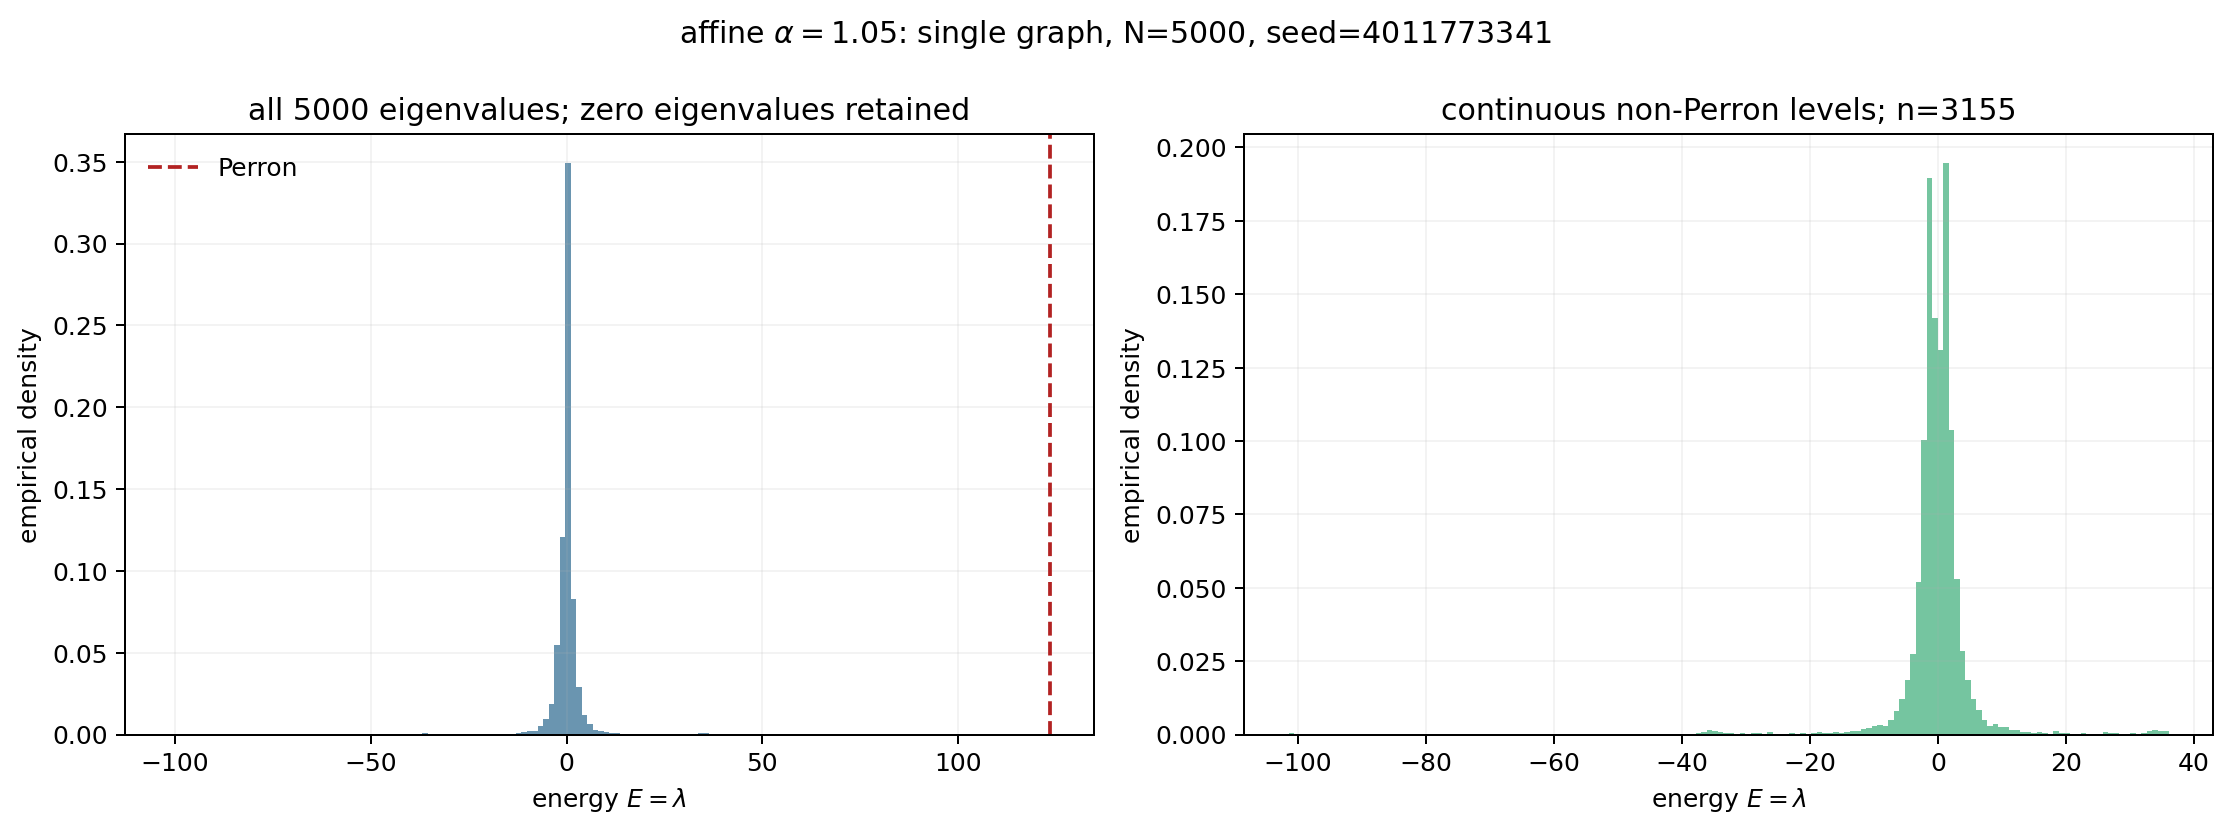
\includegraphics[width=.94\linewidth]{figures/affine_alpha_1p05/spectrum/single_graph_eigenvalue_density.png}
\caption{Original single-graph eigenvalue-density diagnostic for affine $\alpha=1.05$.}\end{figure}
\paragraph{Raw and unfolded local spacing.} The raw histograms vary strongly across energy because the spectral density varies. After local unfolding, most populated interior bins are qualitatively closer to the GOE curve than to the Poisson curve, while the extreme bins contain few gaps and are visibly noisy. The global ratio mean is about 0.531, close to GOE, but that full-spectrum average does not resolve the rank-specific edge fluctuations shown by the microscope.
\begin{figure}[H]\centering
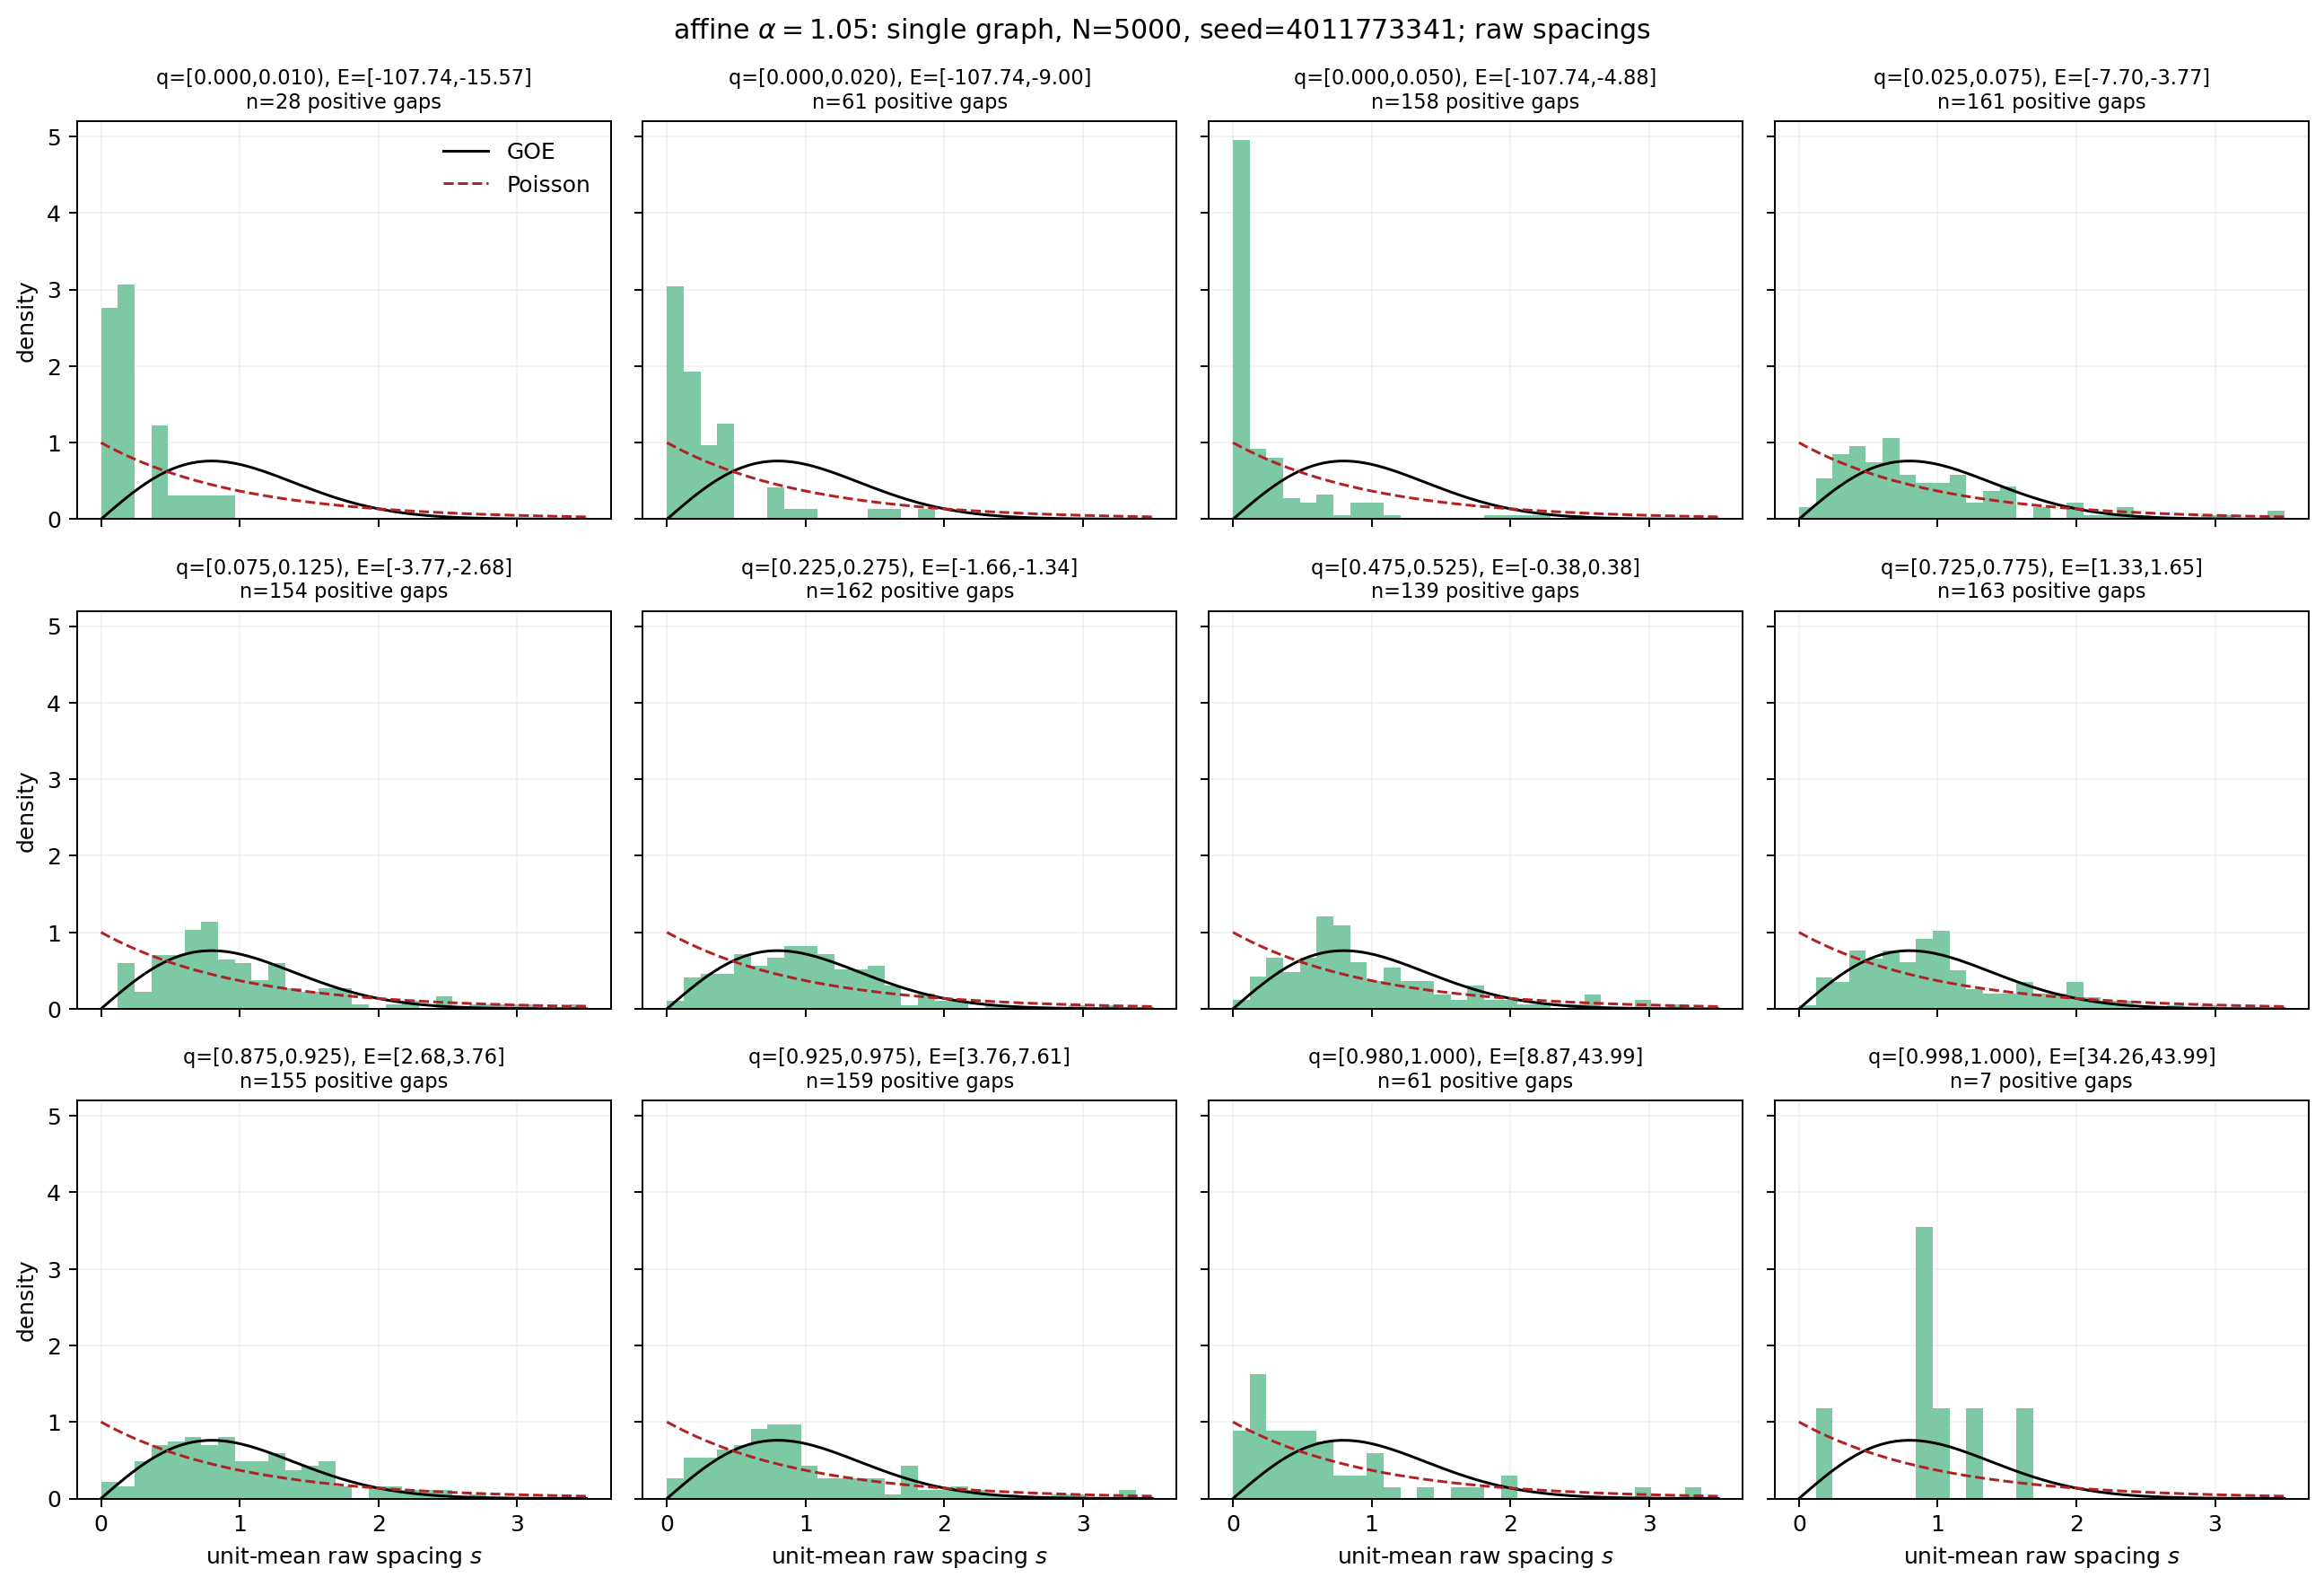
\includegraphics[width=.94\linewidth]{figures/affine_alpha_1p05/histograms/single_graph_local_raw_spacing_histograms.png}
\caption{Original local raw-spacing histograms for affine $\alpha=1.05$.}\end{figure}
\begin{figure}[H]\centering
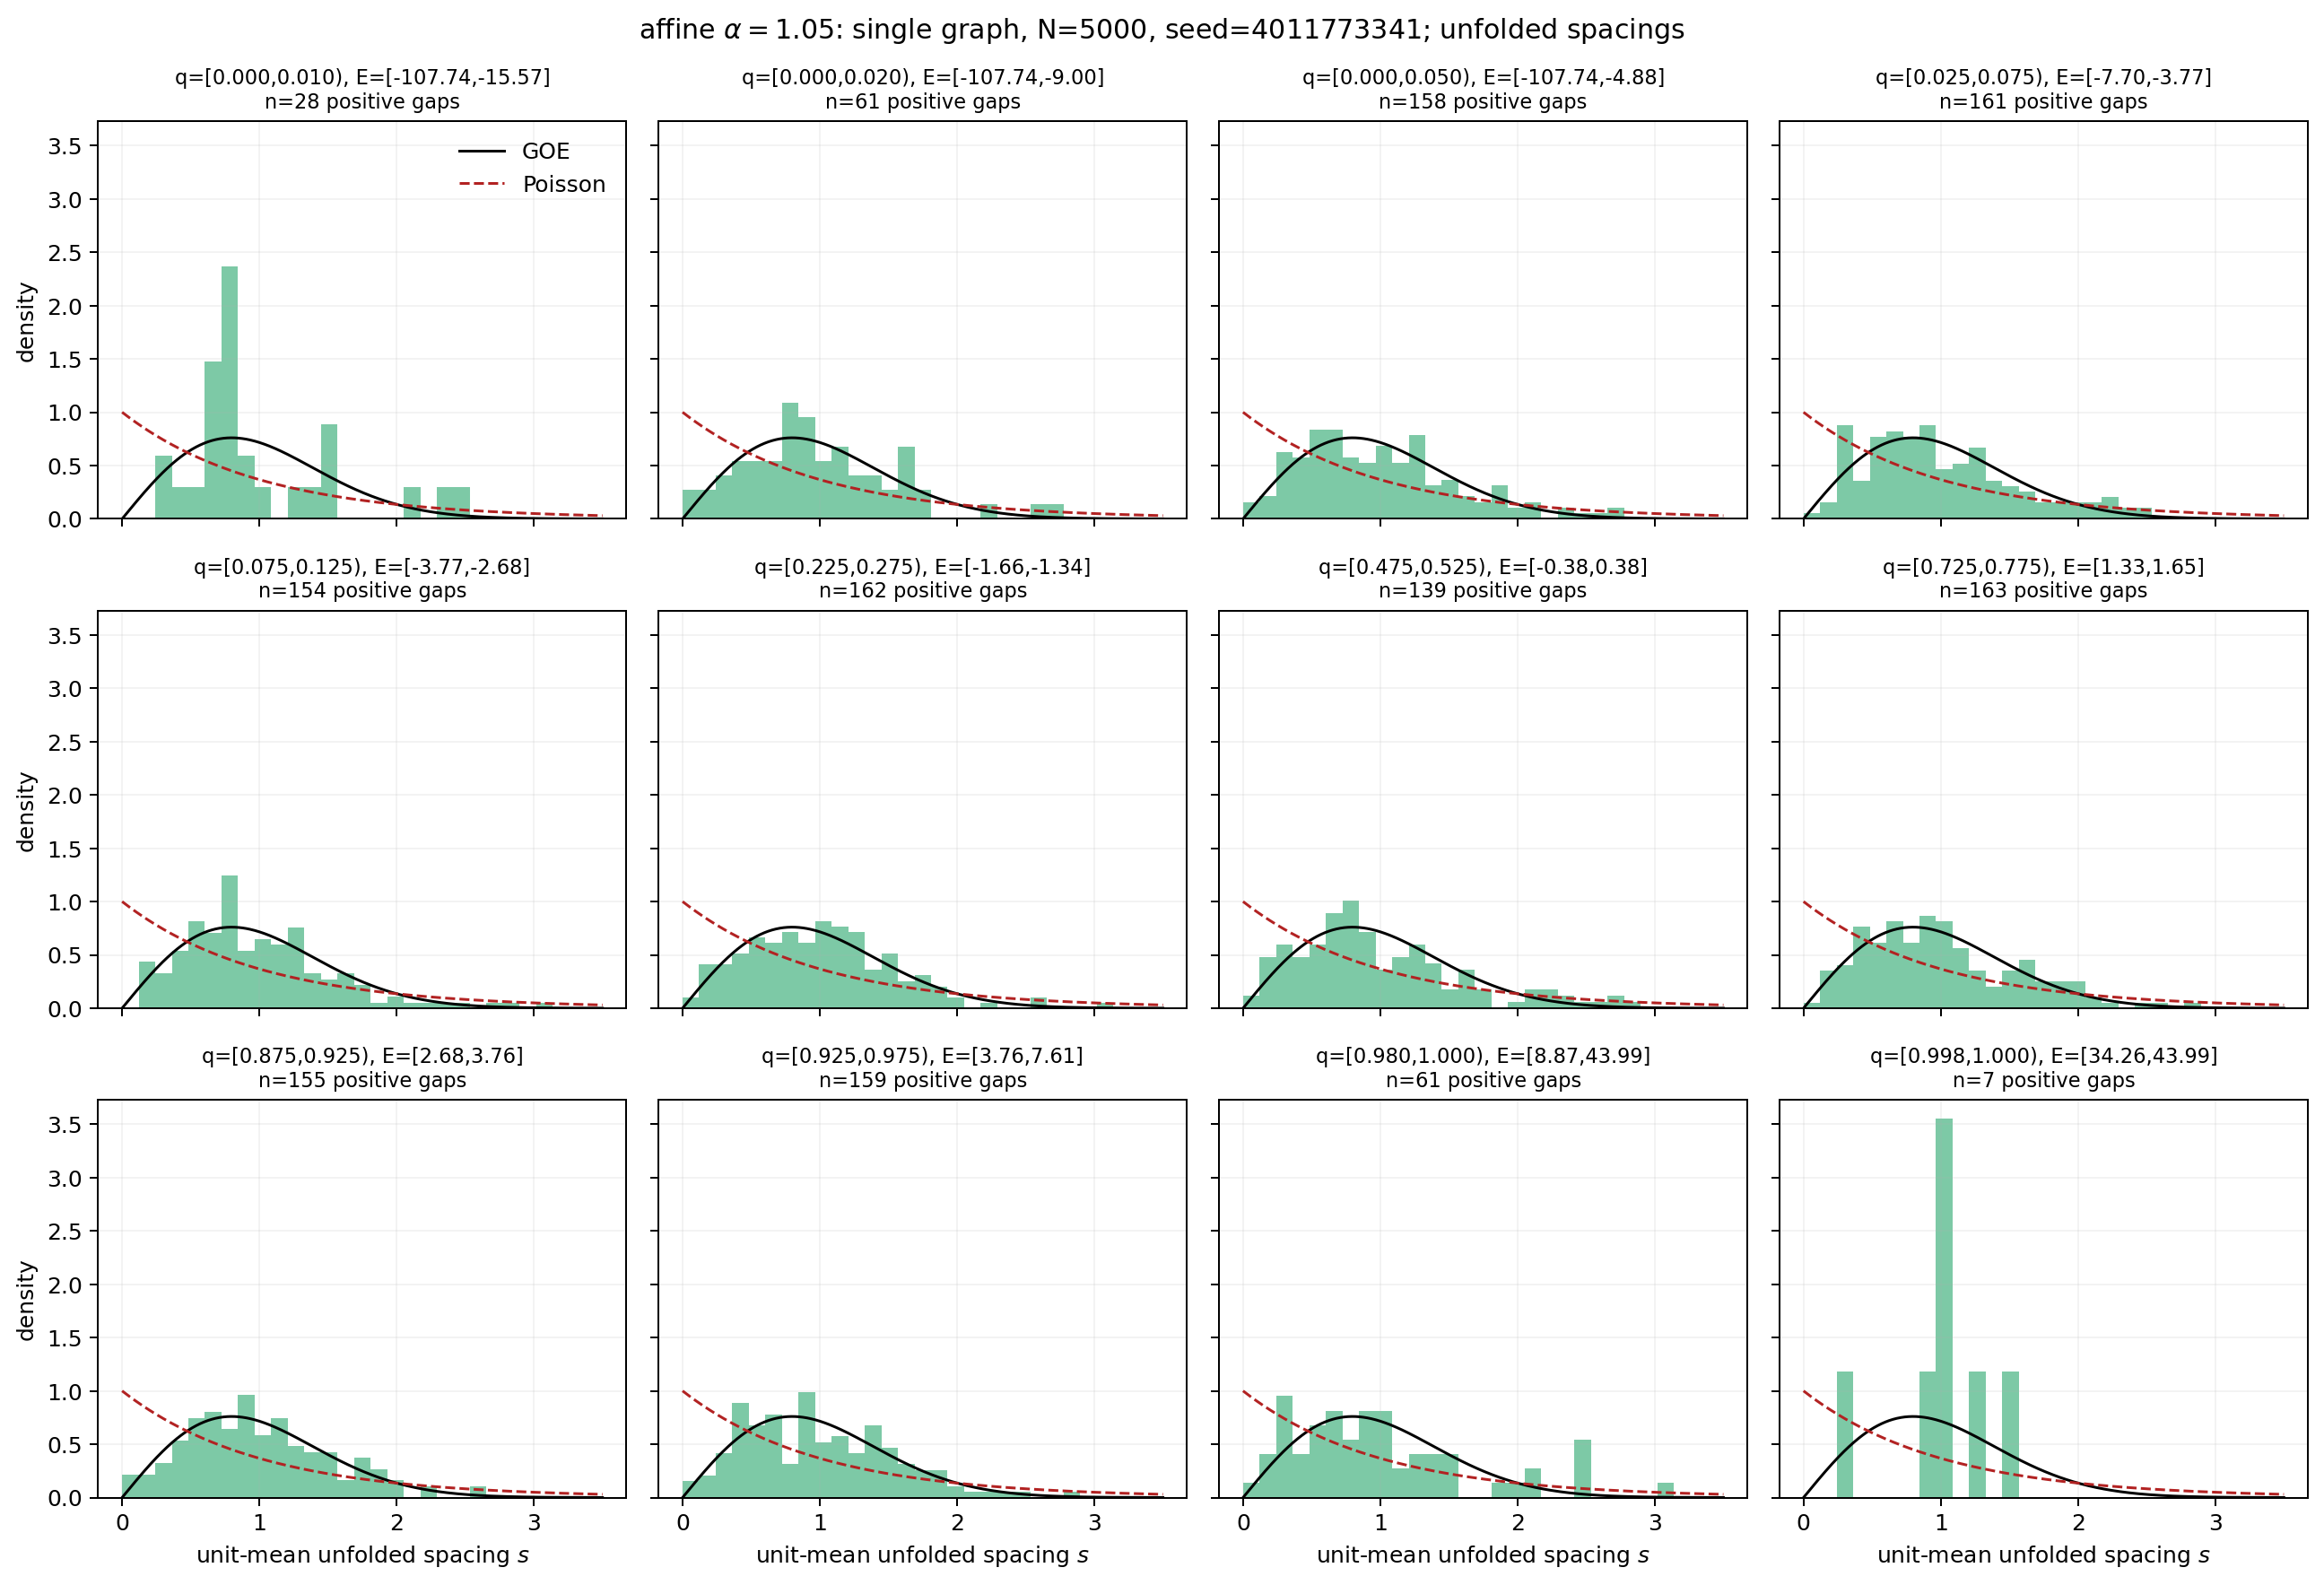
\includegraphics[width=.94\linewidth]{figures/affine_alpha_1p05/histograms/single_graph_local_unfolded_spacing_histograms.png}
\caption{Original local unfolded-spacing histograms for affine $\alpha=1.05$.}\end{figure}
\begin{figure}[H]\centering
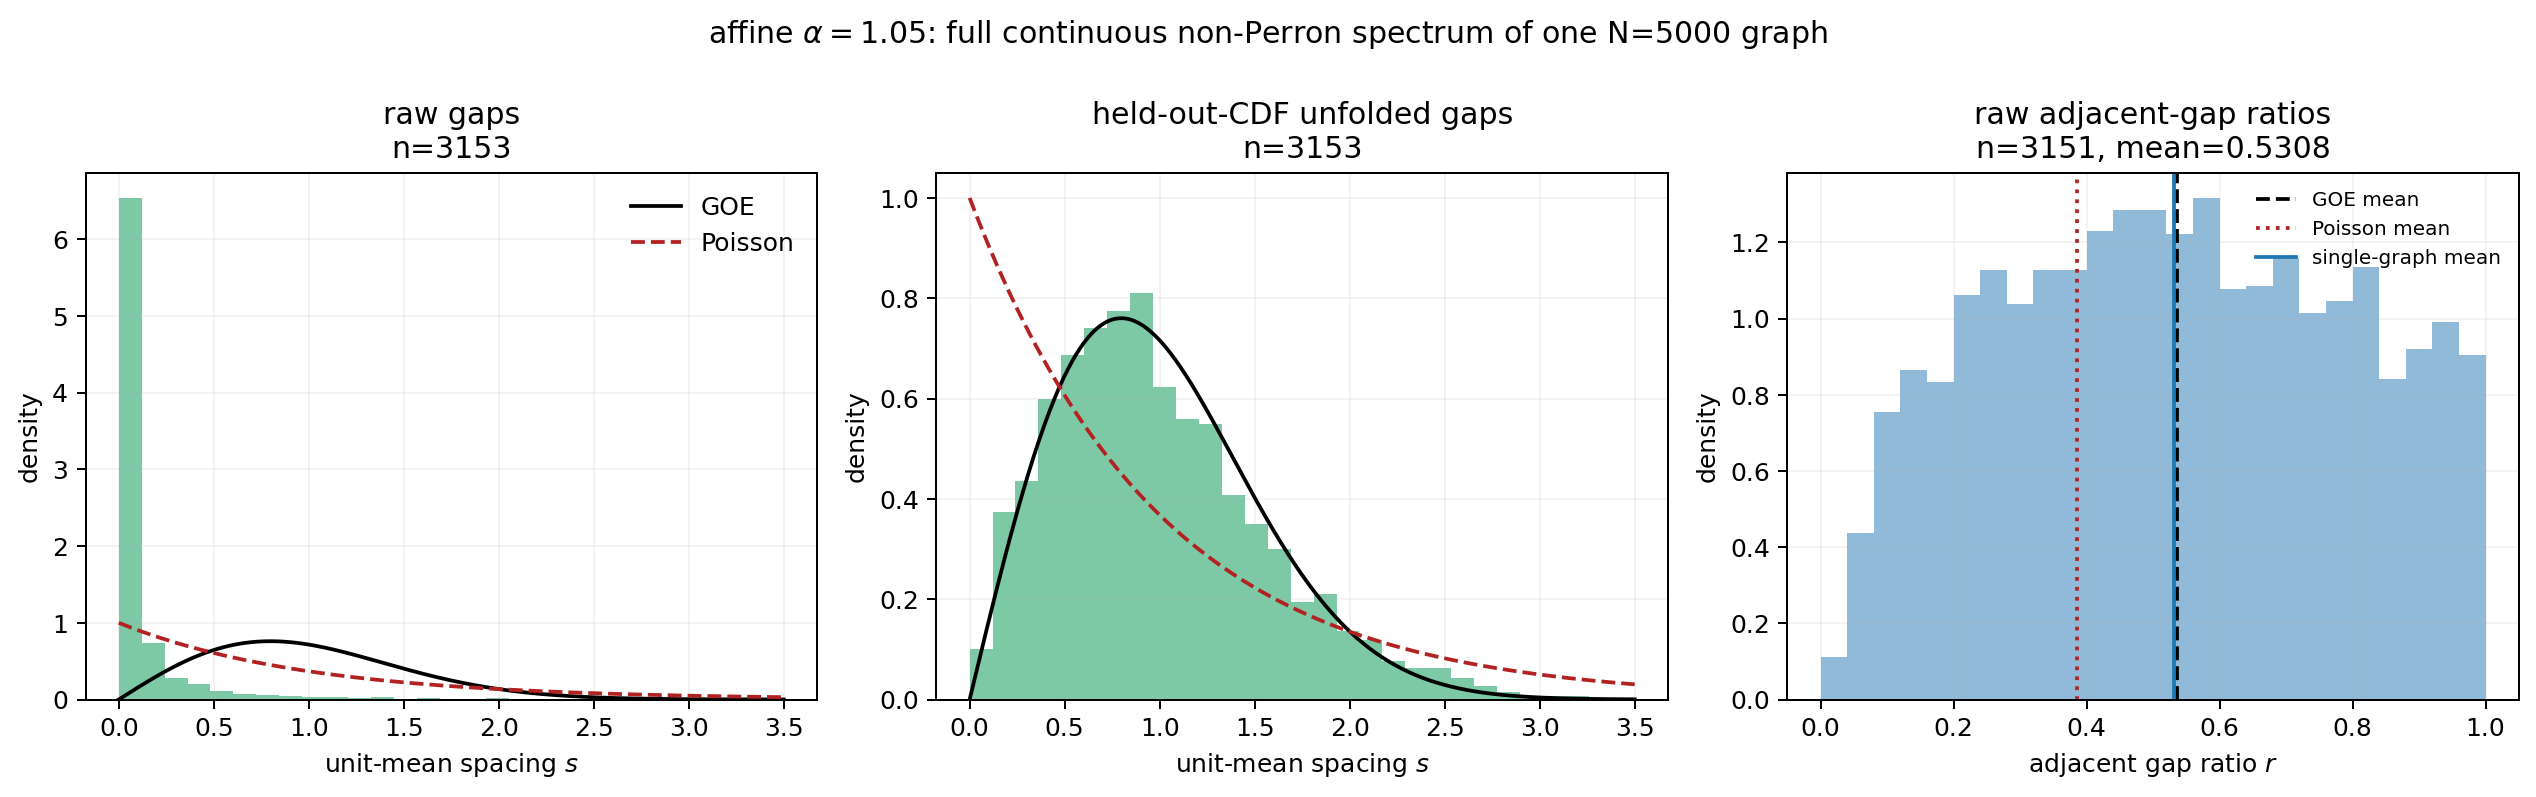
\includegraphics[width=.94\linewidth]{figures/affine_alpha_1p05/histograms/single_graph_global_spacing_and_ratio.png}
\caption{Original full continuous-spectrum spacing and ratio diagnostic for affine $\alpha=1.05$.}\end{figure}
\paragraph{Localization versus energy.} The energy--$N\,\mathrm{IPR}$ cloud has a pronounced localization bowl: the continuous bulk near $E=0$ is least localized, whereas the spectral tails rise by one to two orders of magnitude. The positive-edge rings sit high in the cloud; the isolated far-right Perron point must not be mixed with the non-Perron window summaries.
\begin{figure}[H]\centering
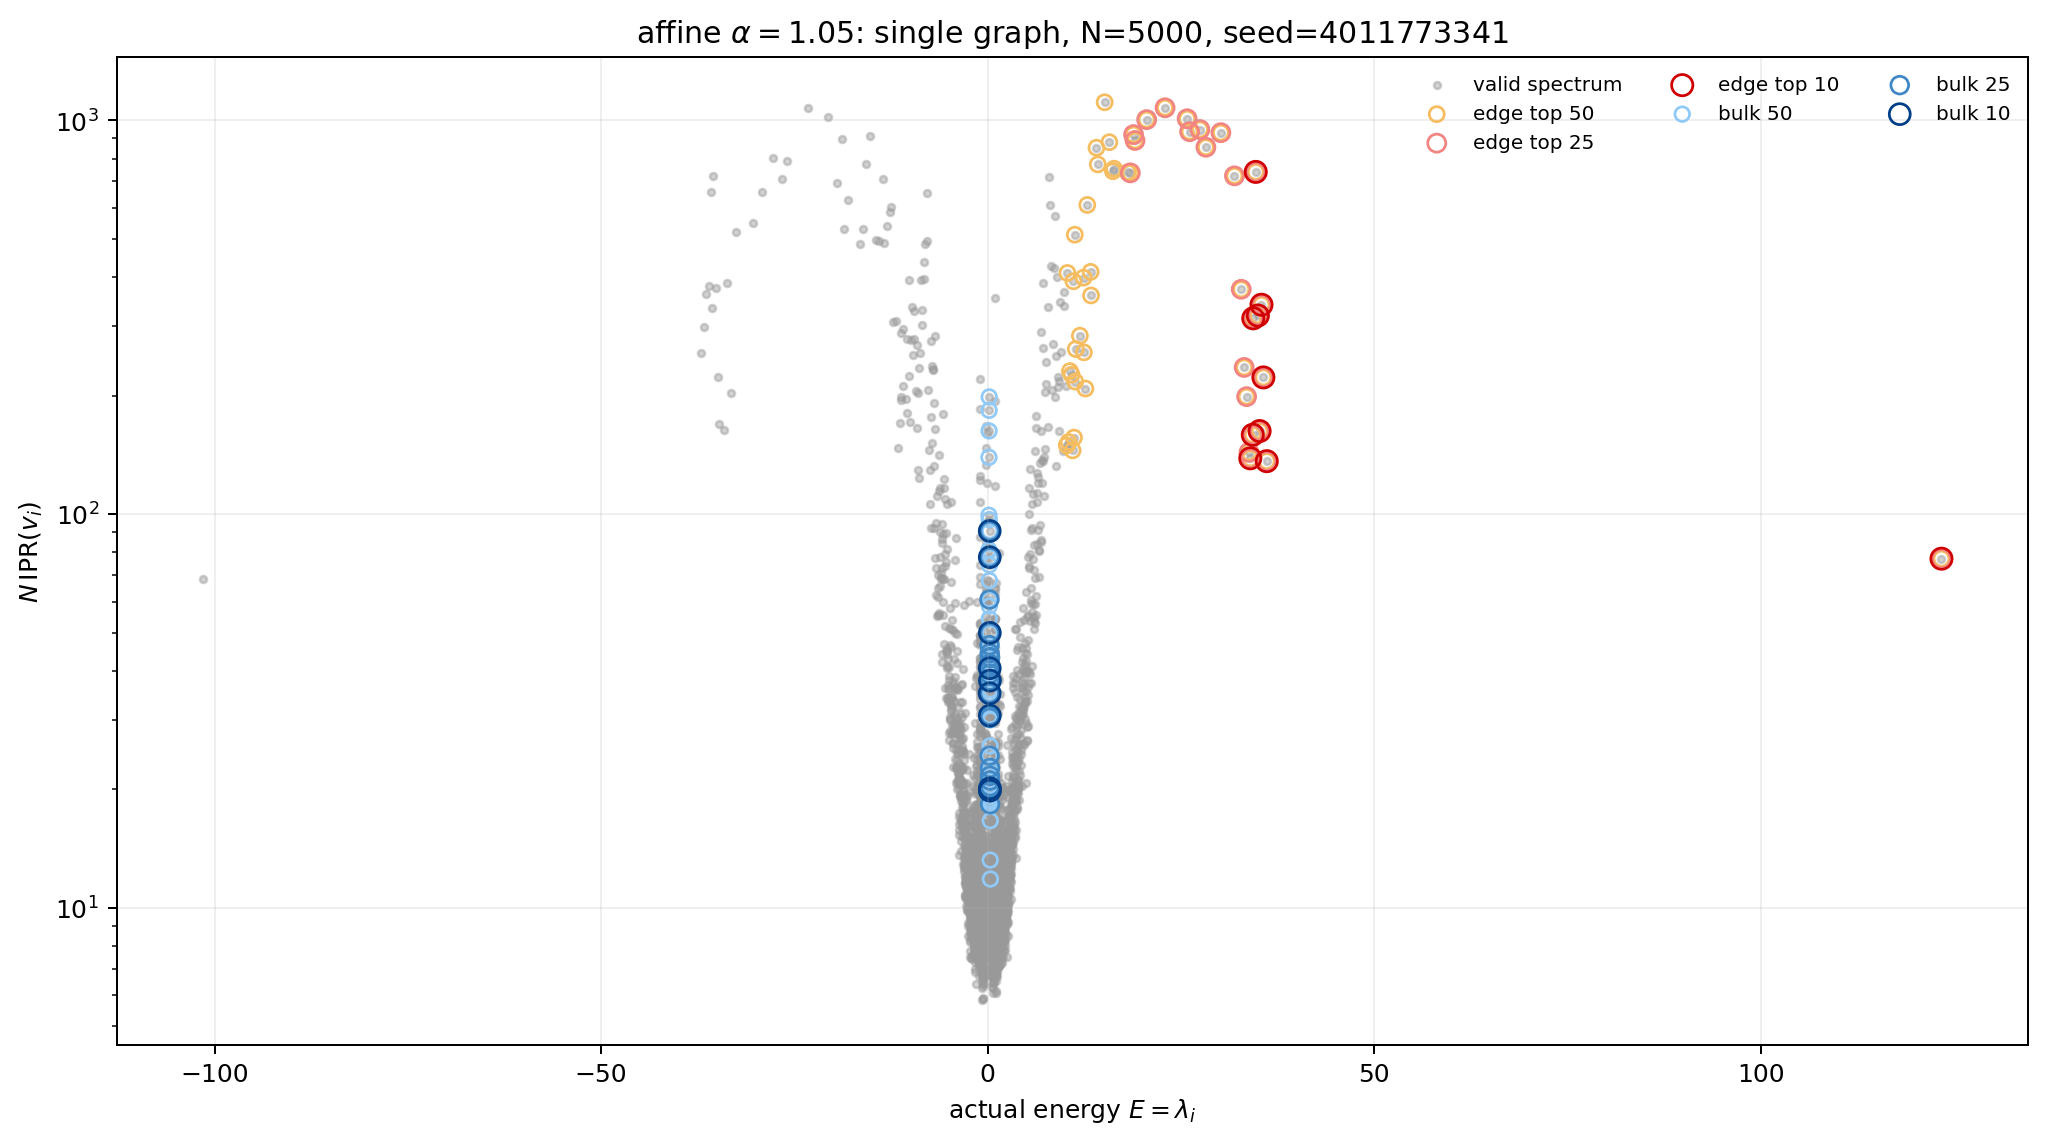
\includegraphics[width=.94\linewidth]{figures/affine_alpha_1p05/energy_ipr/single_graph_localization_vs_energy.png}
\caption{Original localization-versus-energy diagnostic for affine $\alpha=1.05$.}\end{figure}
\paragraph{Edge eigenpair microscope.} Read the four panels together. Individual $r_i$ values oscillate across almost the entire unit interval, so no single point or short run establishes Poisson or GOE statistics. By contrast, $N\,\mathrm{IPR}$ is already in the hundreds near the edge, rises above $10^3$ around ranks 18--31, and remains far above its bulk scale. $M_{10}$ stays near 0.45--0.50 through most of the top 50. The scatter panel shows that very large $N\,\mathrm{IPR}$ occurs at both small and large $r_i$; spacing ratio and localization strength are therefore not monotonically linked.
\begin{figure}[H]\centering
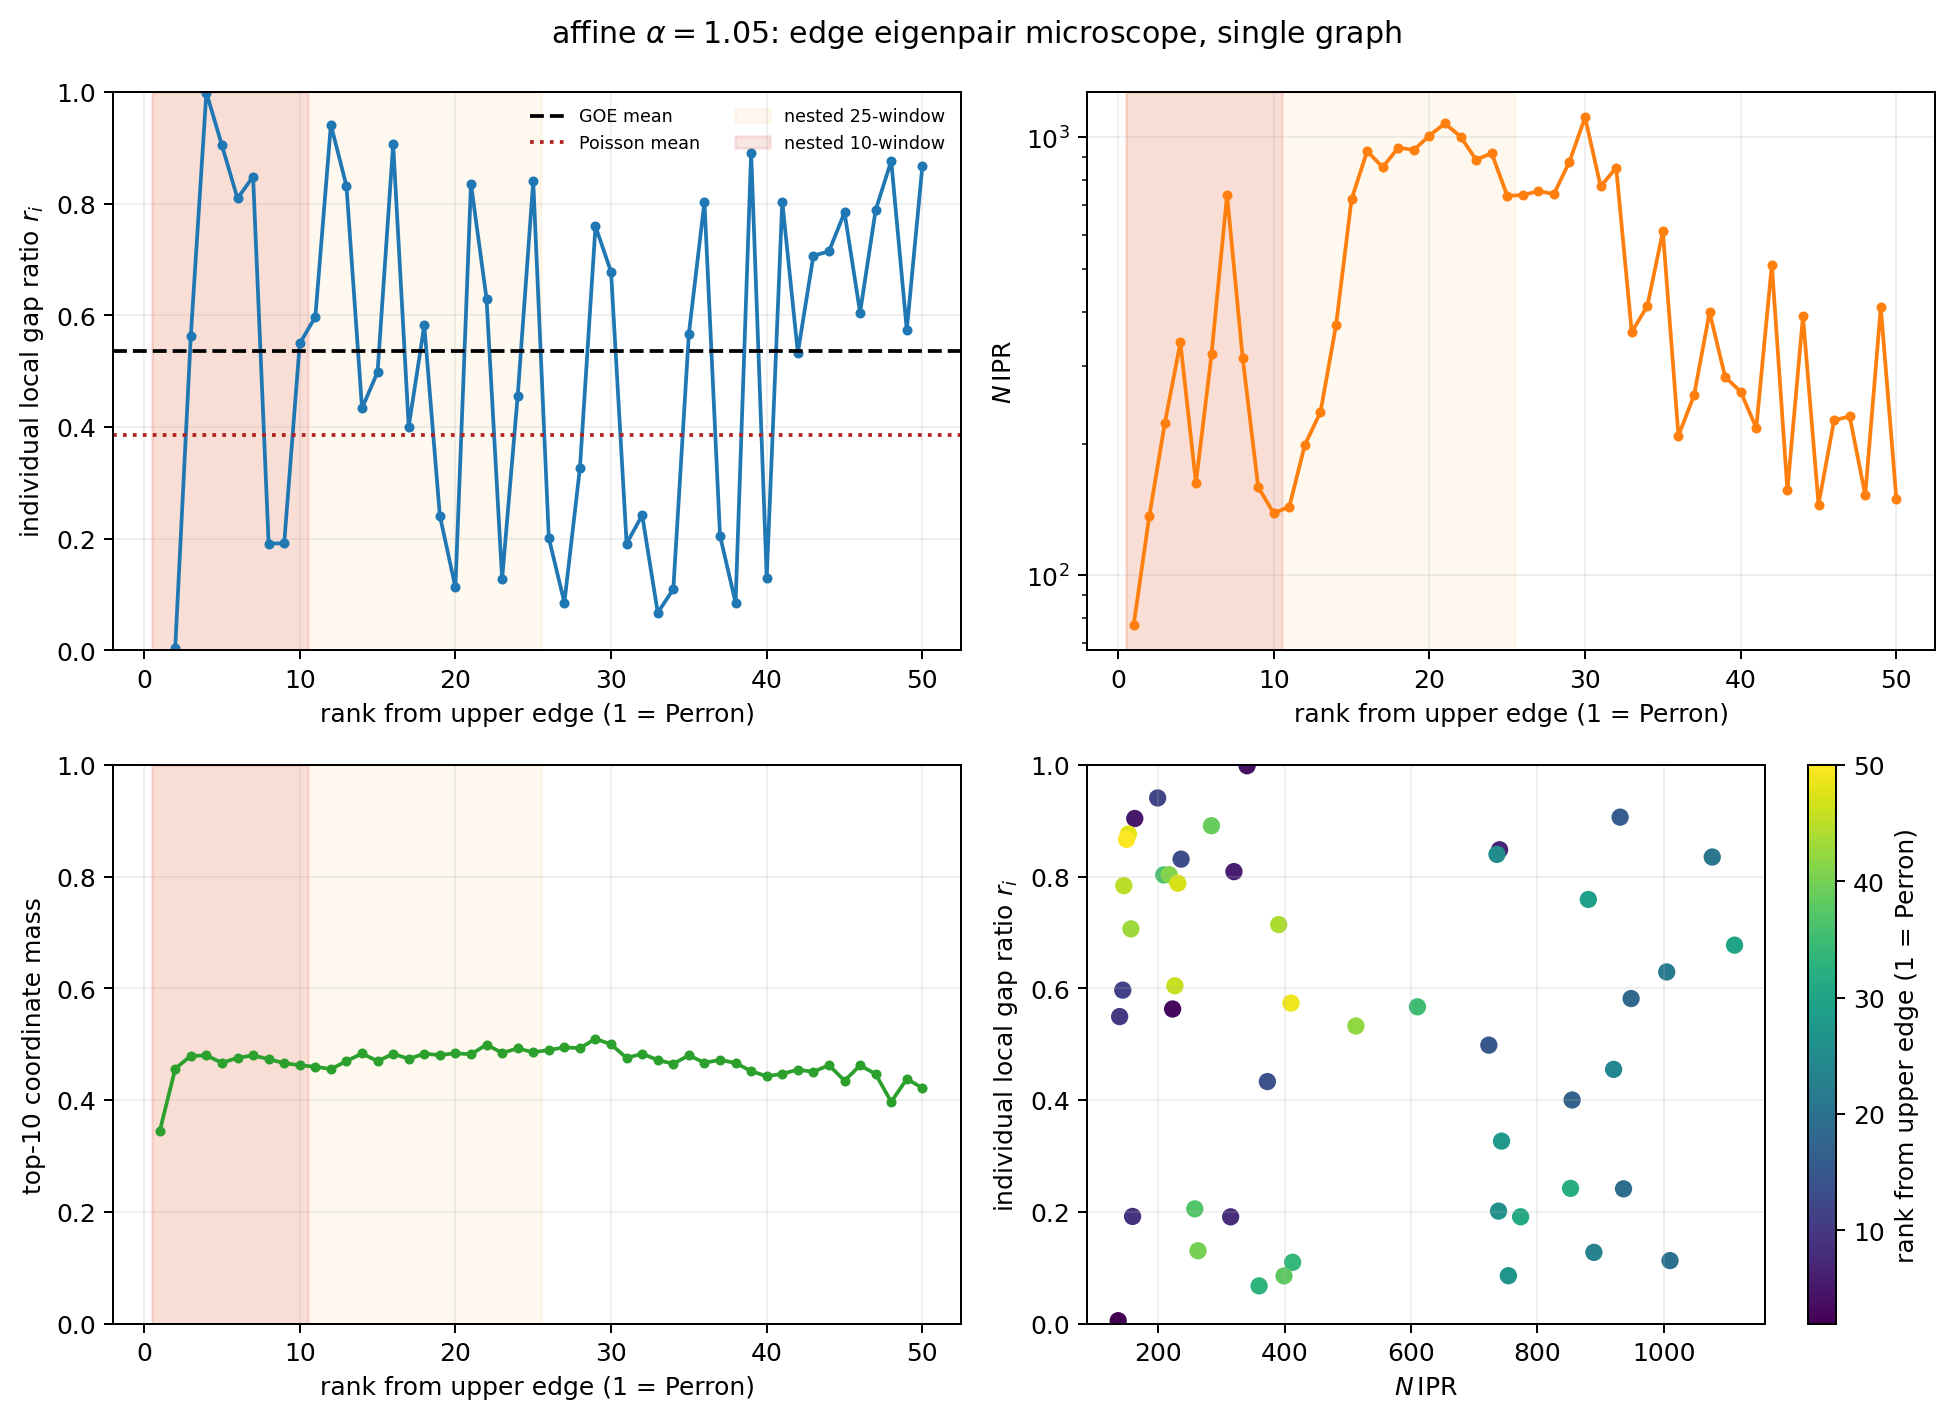
\includegraphics[width=.94\linewidth]{figures/affine_alpha_1p05/edge/edge_rank_diagnostics.png}
\caption{Original four-panel edge-rank eigenpair microscope for affine $\alpha=1.05$.}\end{figure}
\paragraph{Bulk eigenpair microscope.} The centered zero-eigenvalue-free bulk still has irregular pointwise $r_i$, but its localization measures are much smaller: $N\,\mathrm{IPR}$ is mostly in the tens and $M_{10}$ is generally about 0.1--0.3 near the selected center. The larger values at negative offsets show that the chosen 50-level display spans a localization gradient; the nested numerical tables are the controlled comparison.
\begin{figure}[H]\centering
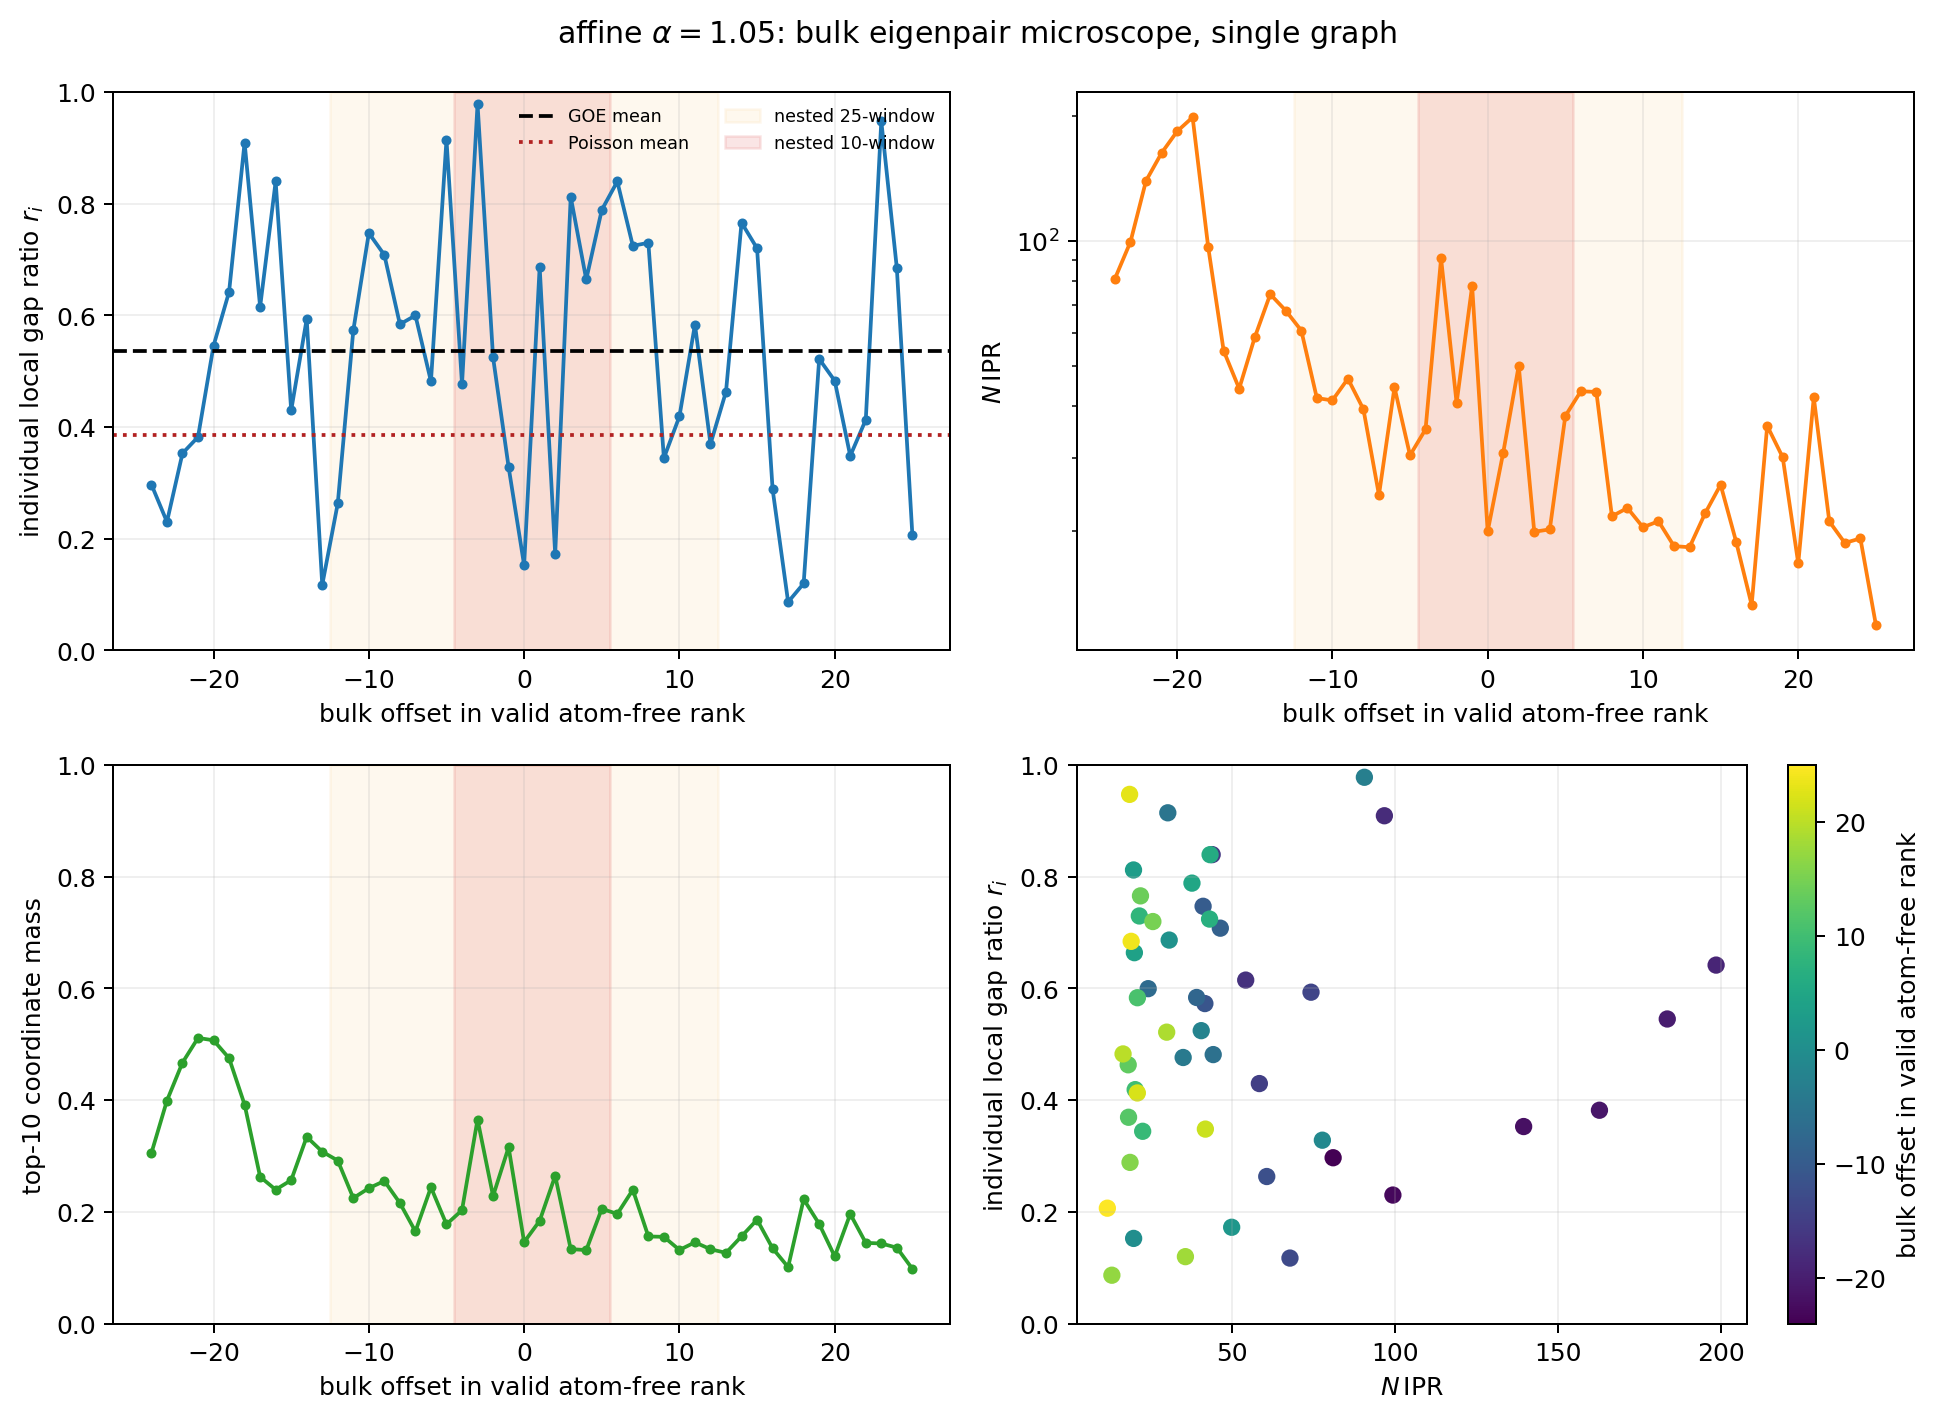
\includegraphics[width=.94\linewidth]{figures/affine_alpha_1p05/bulk/bulk_offset_diagnostics.png}
\caption{Original four-panel centered bulk-offset eigenpair microscope for affine $\alpha=1.05$.}\end{figure}
\paragraph{Direct edge-versus-bulk comparison.} The boxplots separate edge from bulk most clearly in $N\,\mathrm{IPR}$, $M_{10}$, top-support degree, induced density, and full-graph distance. Edge supports range from very dense hub cores to less dense deeper states, whereas bulk supports cluster near zero density. The edge distance z-scores are strongly negative, meaning substantially shorter paths than uniformly random ten-vertex sets.
\begin{figure}[H]\centering
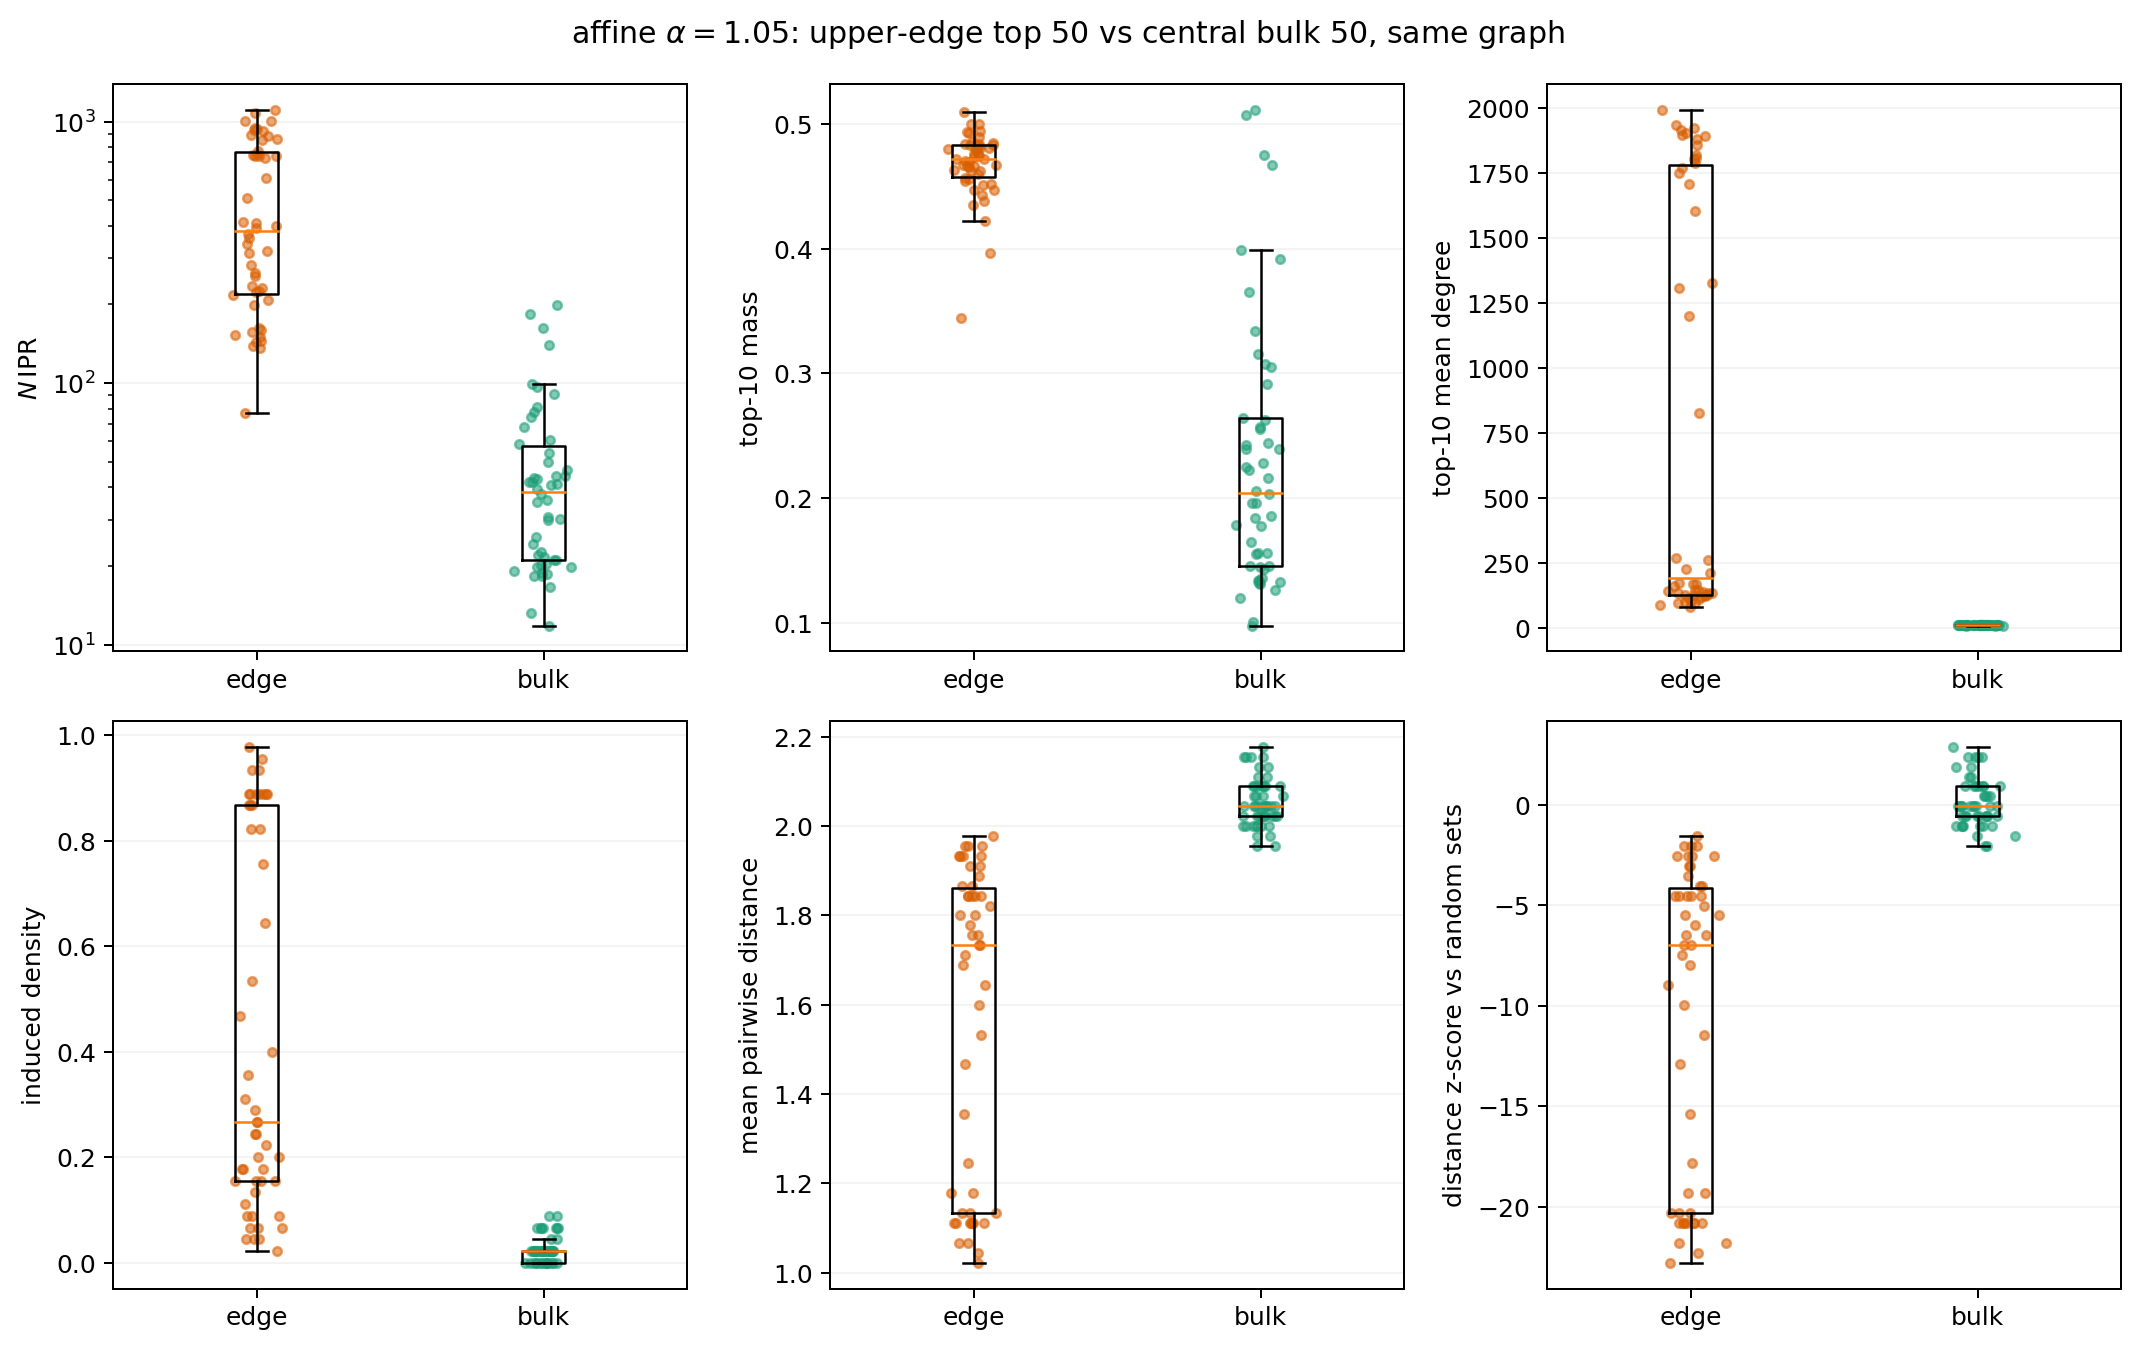
\includegraphics[width=.94\linewidth]{figures/affine_alpha_1p05/edge_vs_bulk/edge_vs_bulk_comparison.png}
\caption{Original direct edge-versus-bulk comparison for affine $\alpha=1.05$.}\end{figure}
\subsection{nonlinear $\zeta=1.5$}
\paragraph{Eigenvalue density.} The full spectrum contains a smaller but still visible block of repeated zero eigenvalues. Removing those eigenvalues and the Perron root produces 4,759 continuous non-Perron levels. As in the affine stress case, the sharp central density peak makes raw gaps near zero small without implying localization on its own.
\begin{figure}[H]\centering
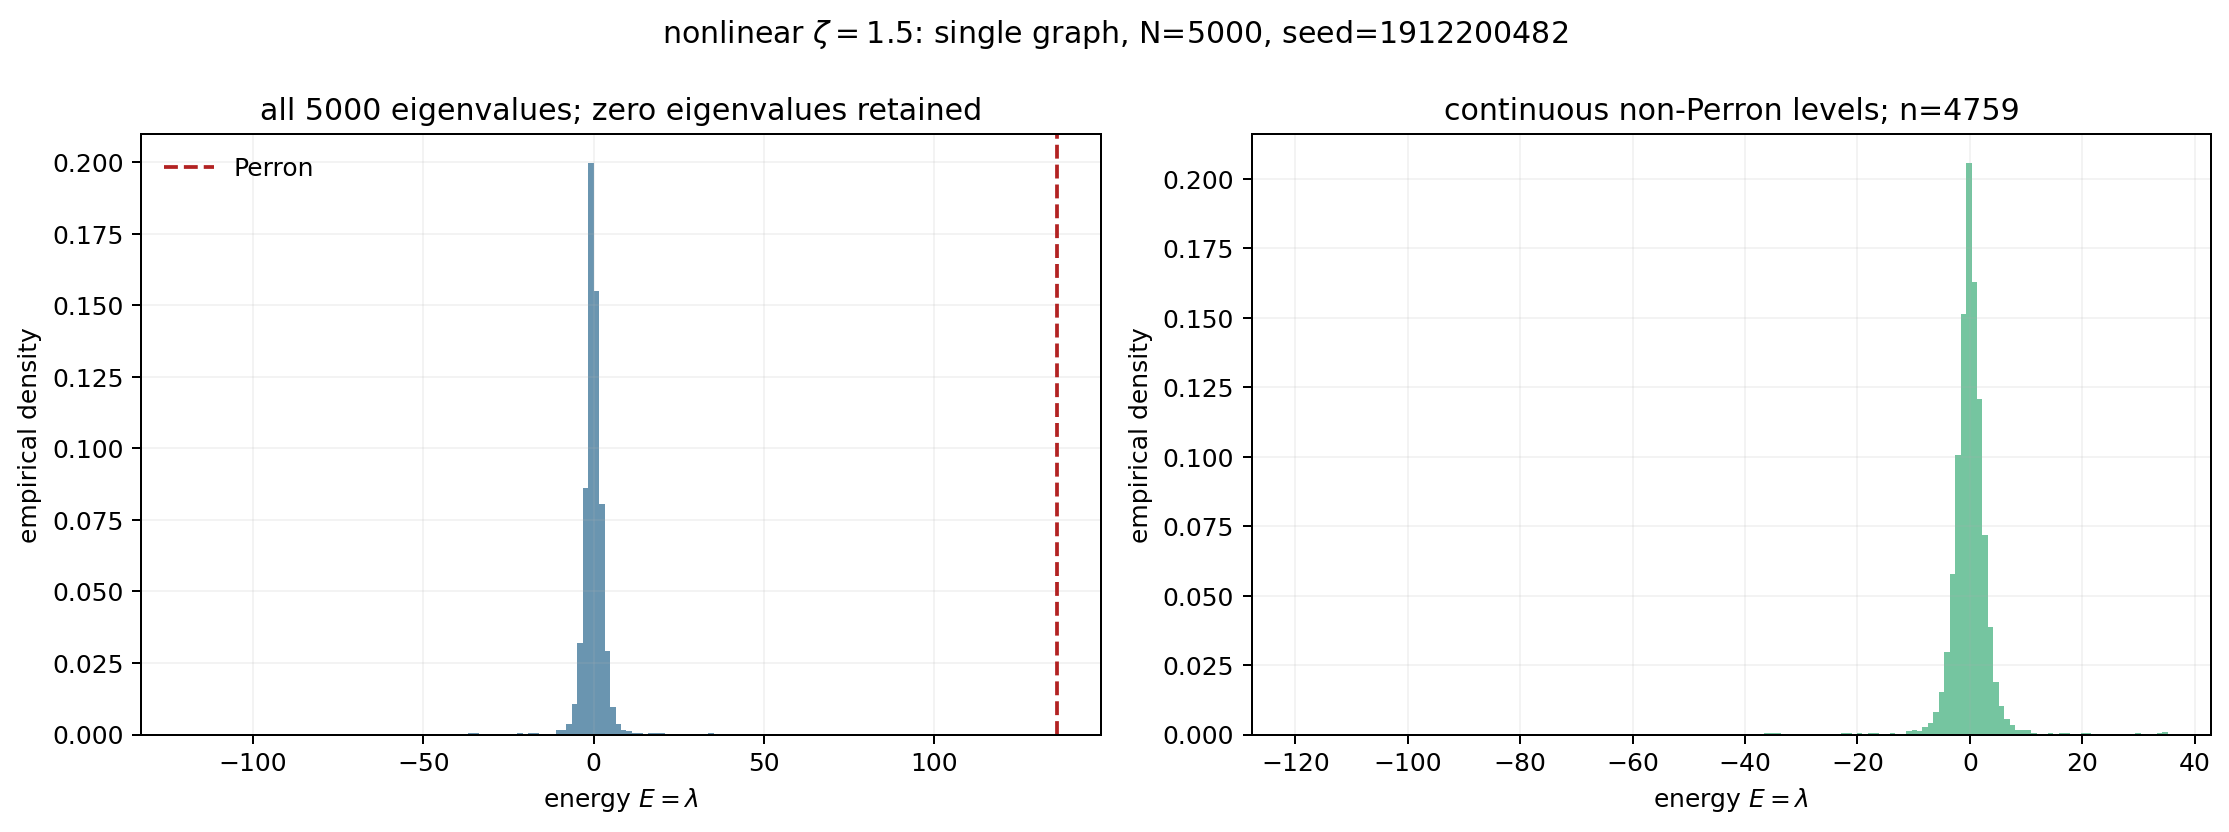
\includegraphics[width=.94\linewidth]{figures/nonlinear_zeta_1p5/spectrum/single_graph_eigenvalue_density.png}
\caption{Original single-graph eigenvalue-density diagnostic for nonlinear $\zeta=1.5$.}\end{figure}
\paragraph{Raw and unfolded local spacing.} Unfolding largely removes the energy-dependent gap scale. The well-populated interior panels are closer to the GOE shape than to the exponential Poisson reference; the outermost panels have only tens of gaps and should be read as descriptive. The full continuous-spectrum ratio mean is about 0.536, while the non-Perron top-10 strict mean is 0.387. That contrast is a narrow-edge effect, not a whole-spectrum Poisson regime.
\begin{figure}[H]\centering
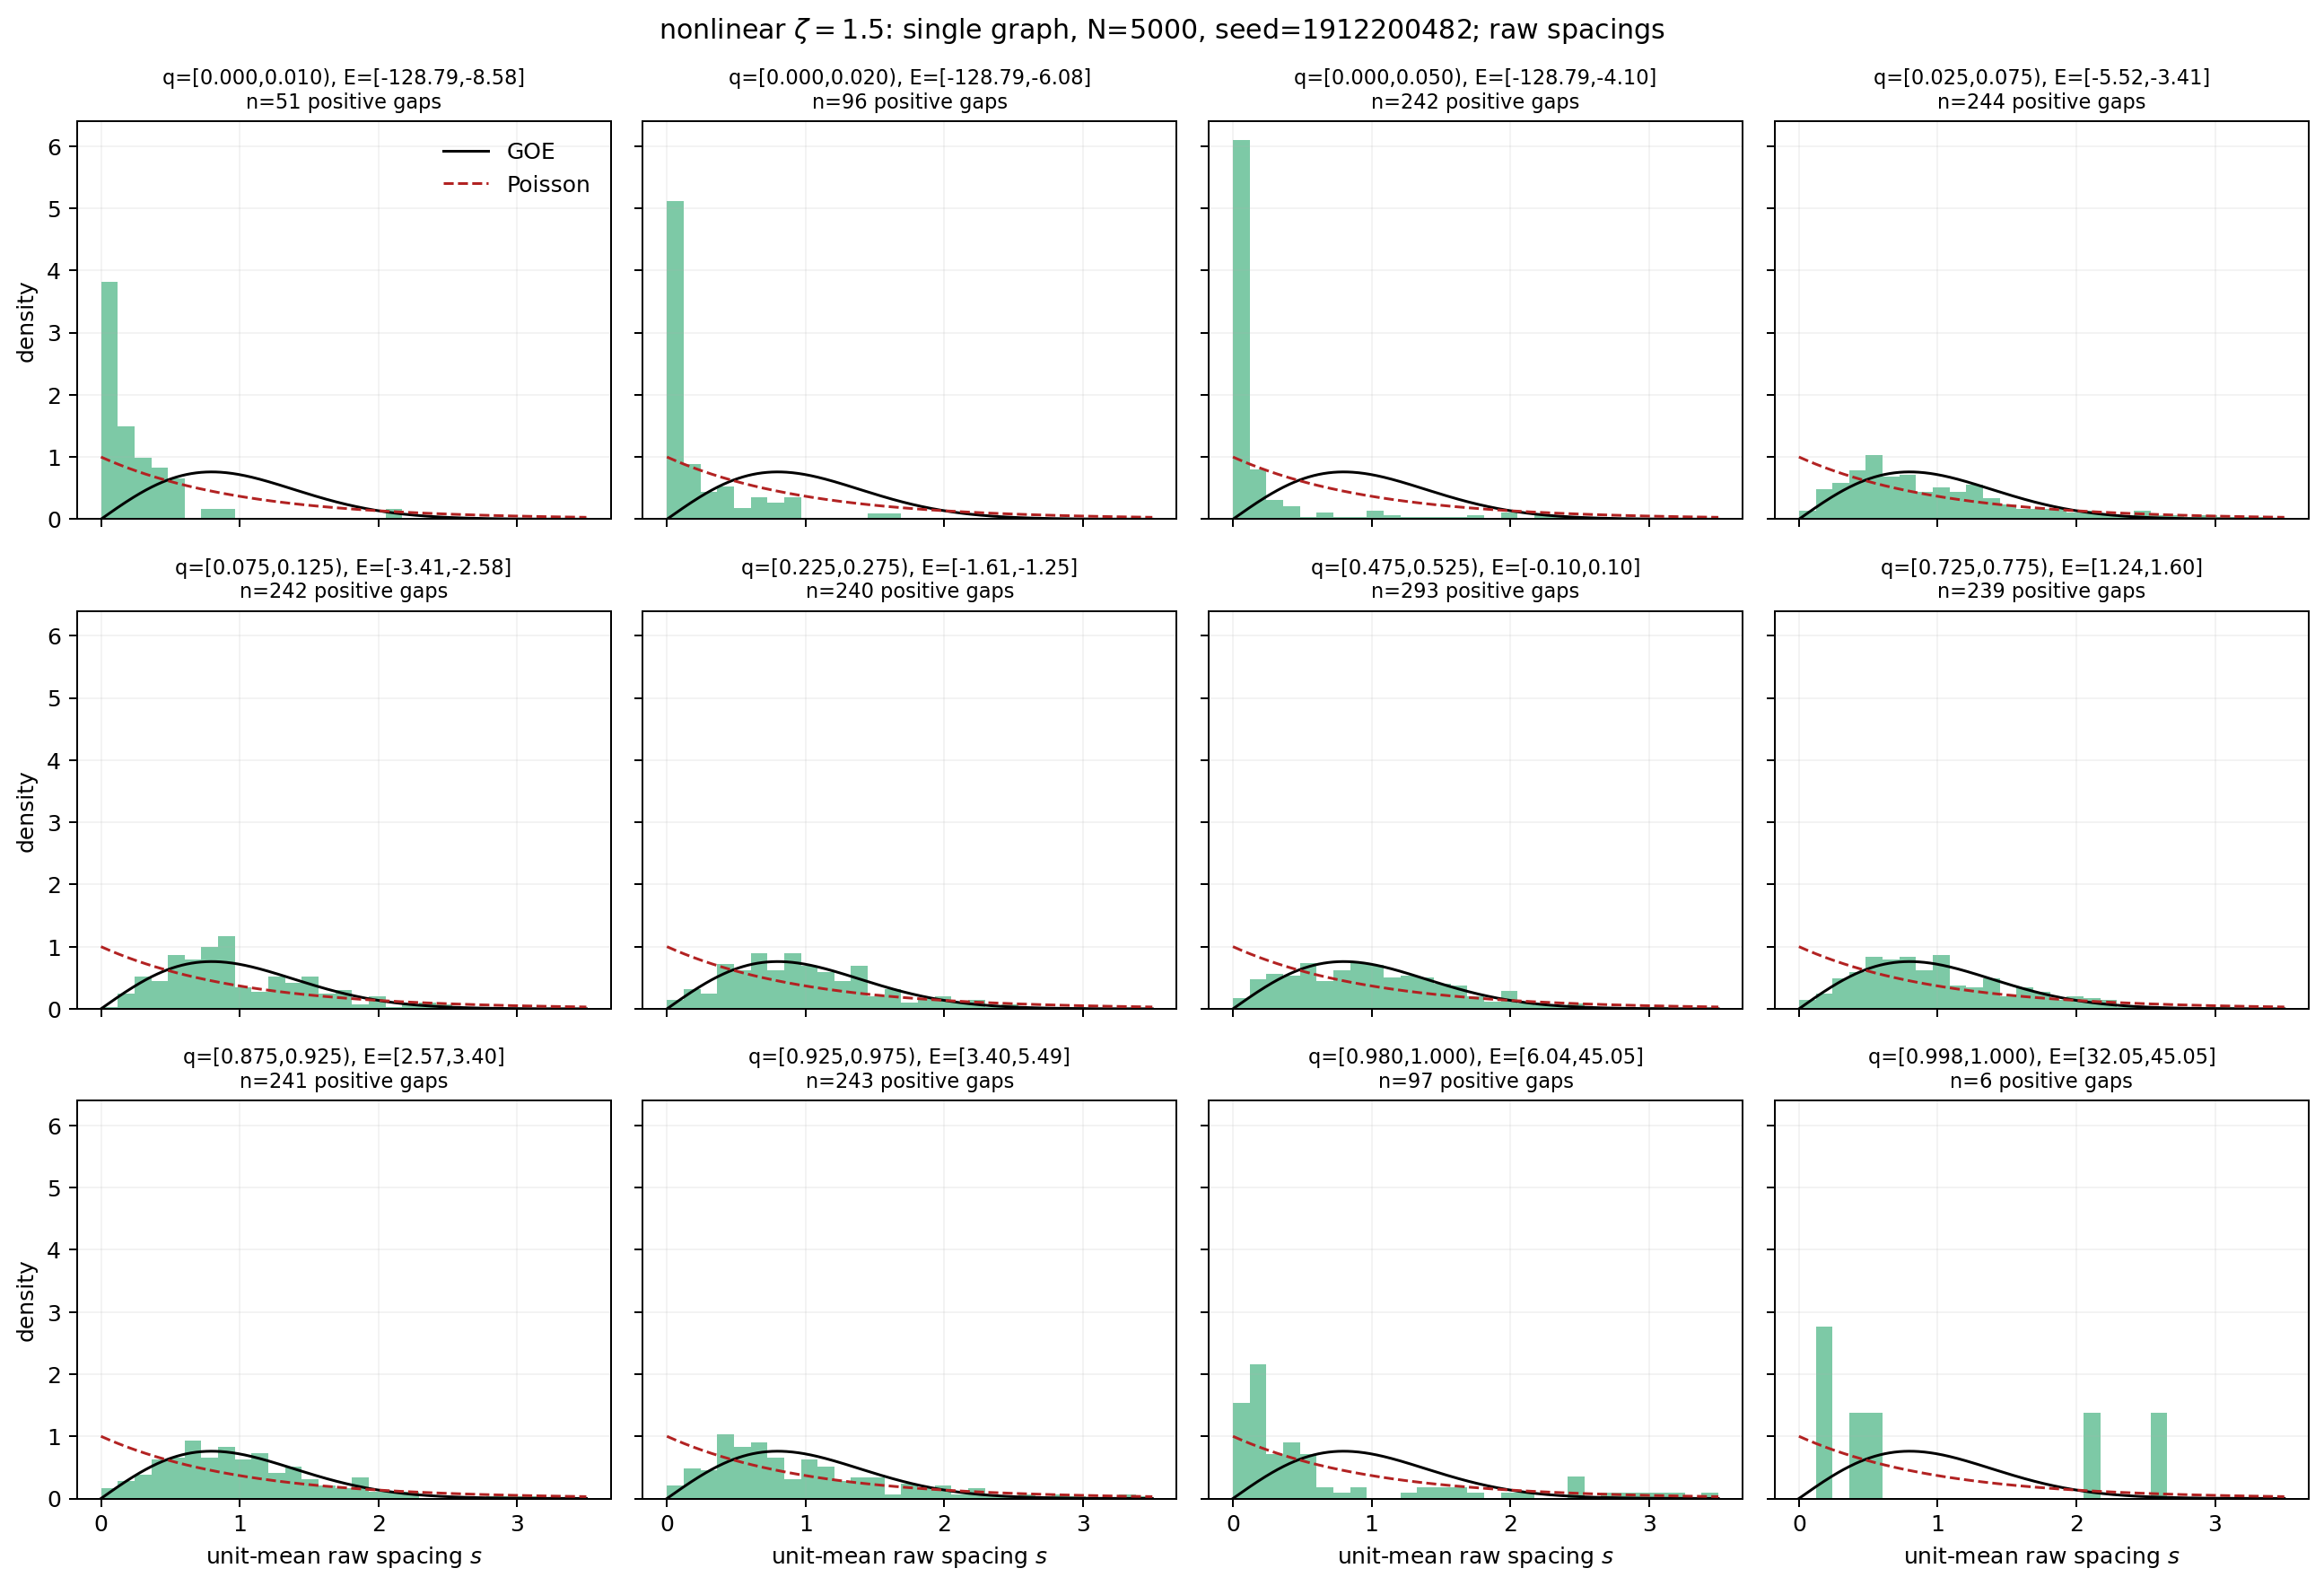
\includegraphics[width=.94\linewidth]{figures/nonlinear_zeta_1p5/histograms/single_graph_local_raw_spacing_histograms.png}
\caption{Original local raw-spacing histograms for nonlinear $\zeta=1.5$.}\end{figure}
\begin{figure}[H]\centering
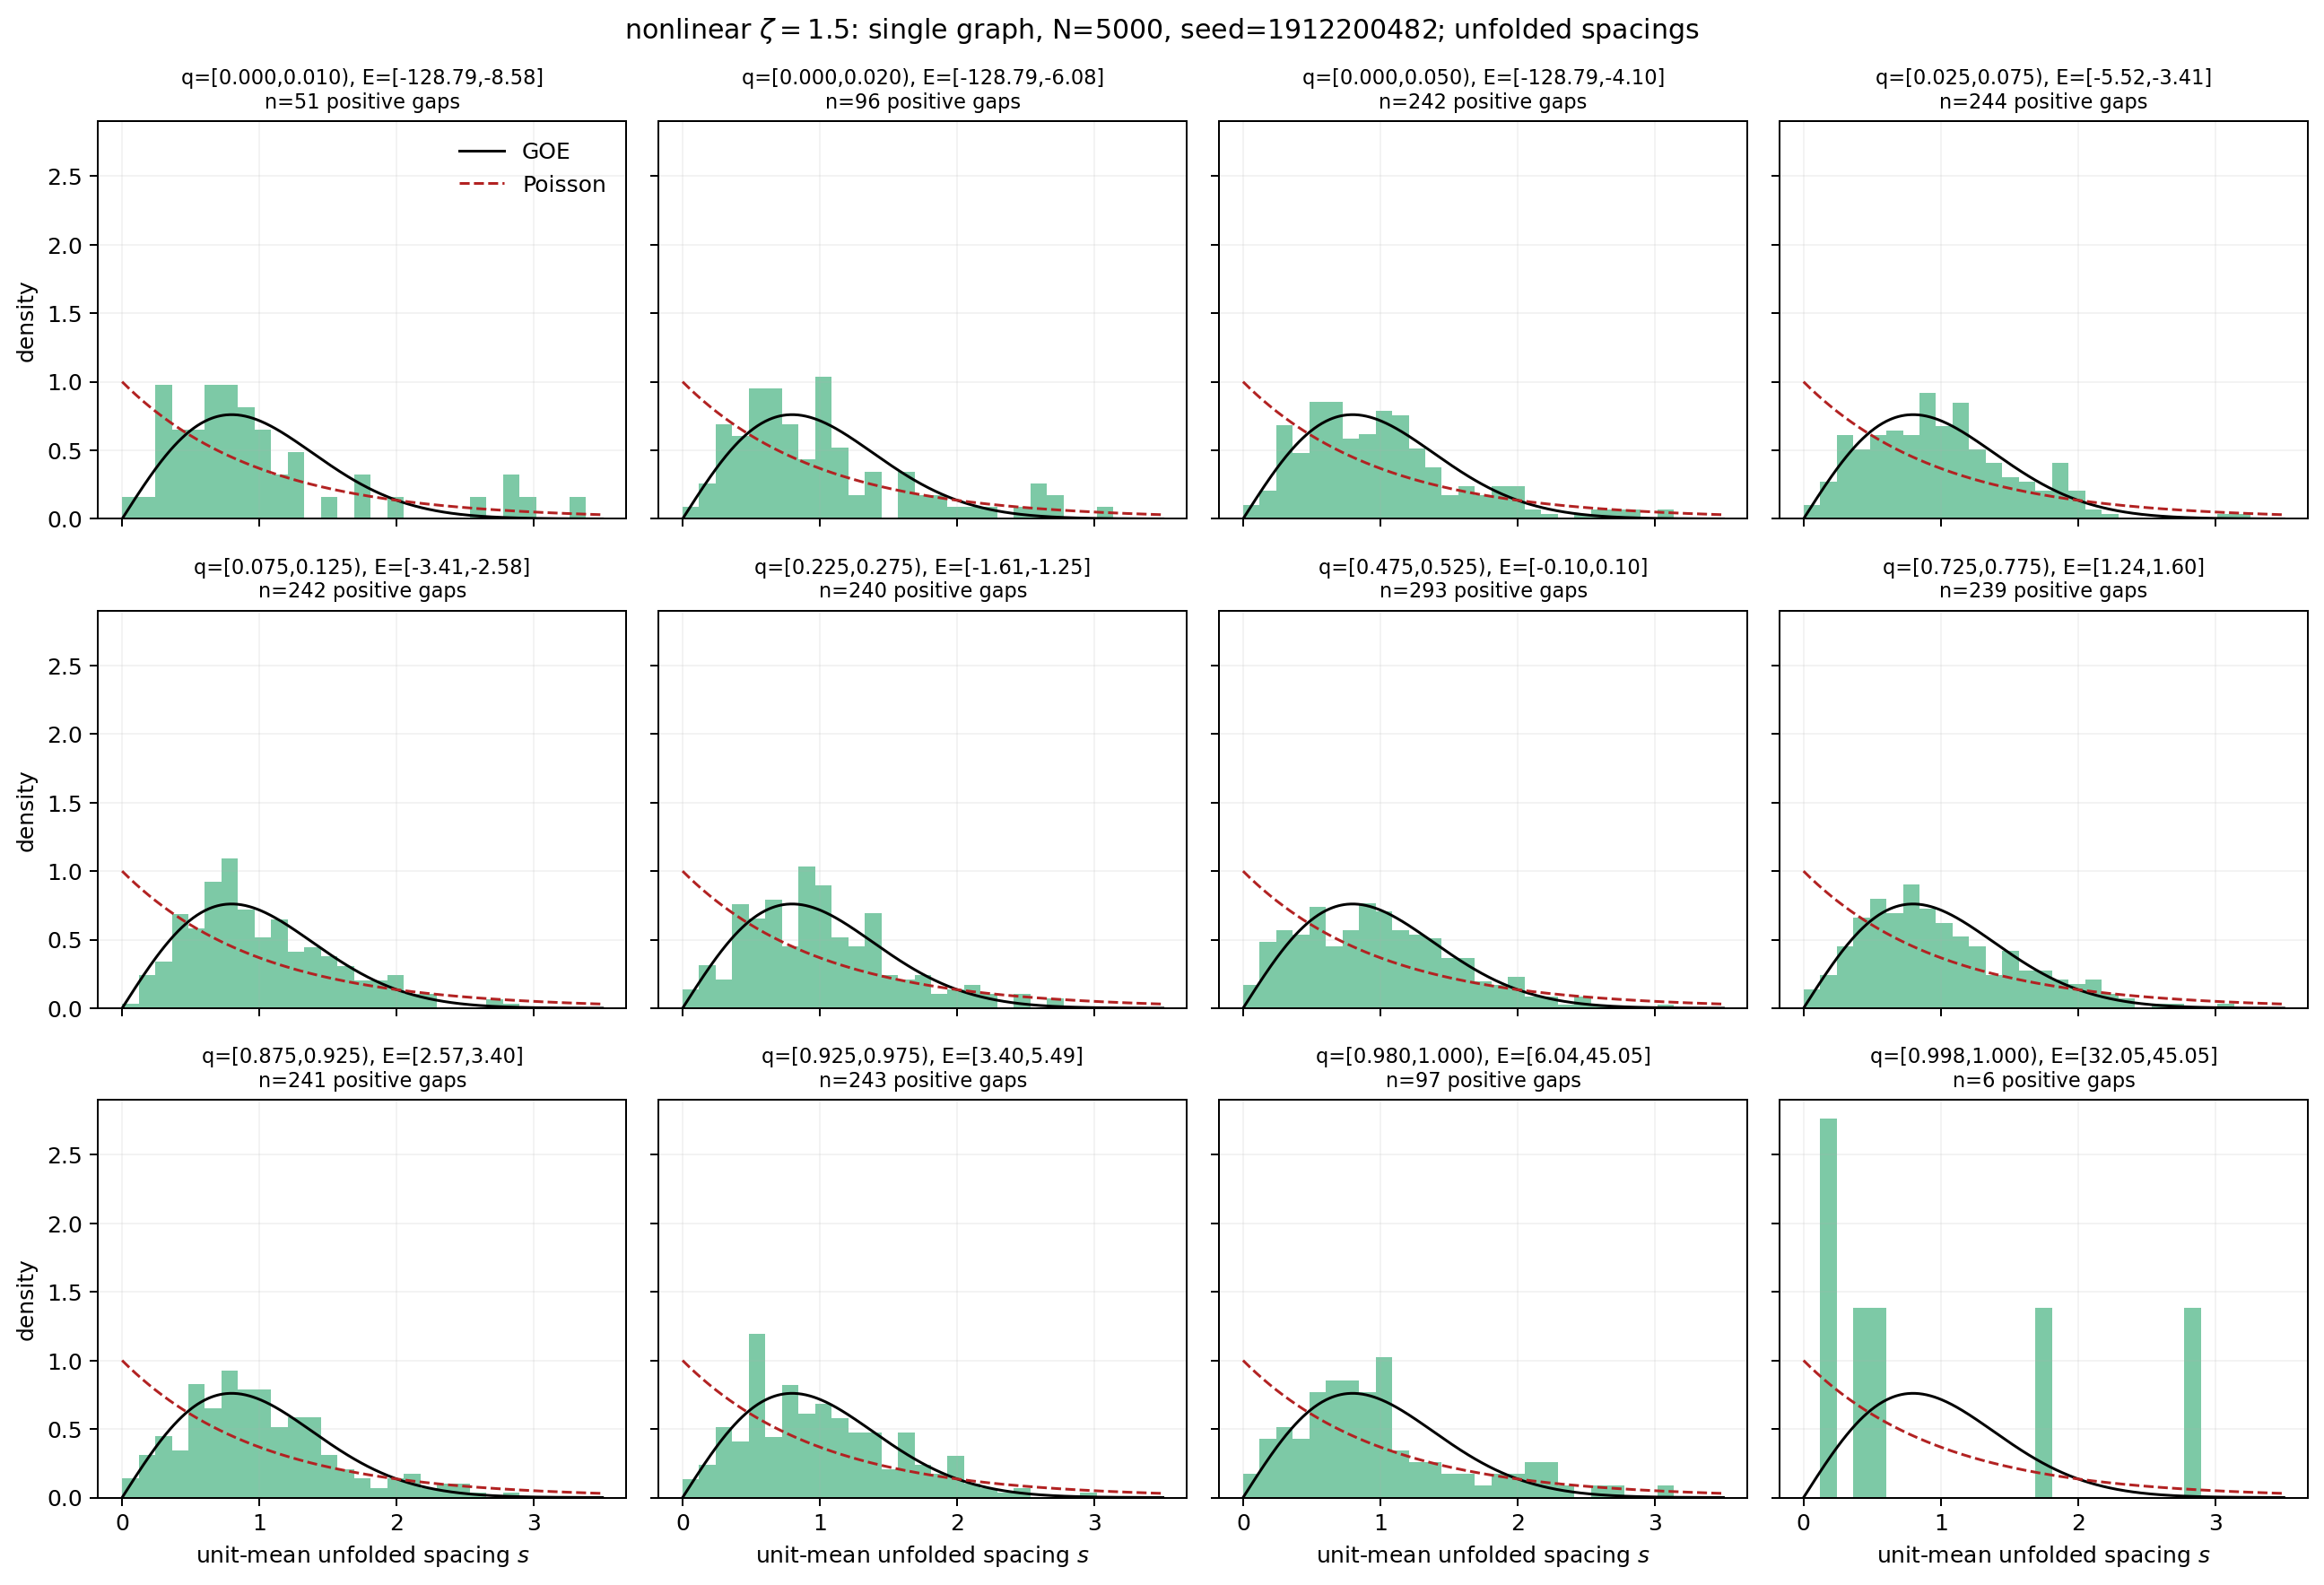
\includegraphics[width=.94\linewidth]{figures/nonlinear_zeta_1p5/histograms/single_graph_local_unfolded_spacing_histograms.png}
\caption{Original local unfolded-spacing histograms for nonlinear $\zeta=1.5$.}\end{figure}
\begin{figure}[H]\centering
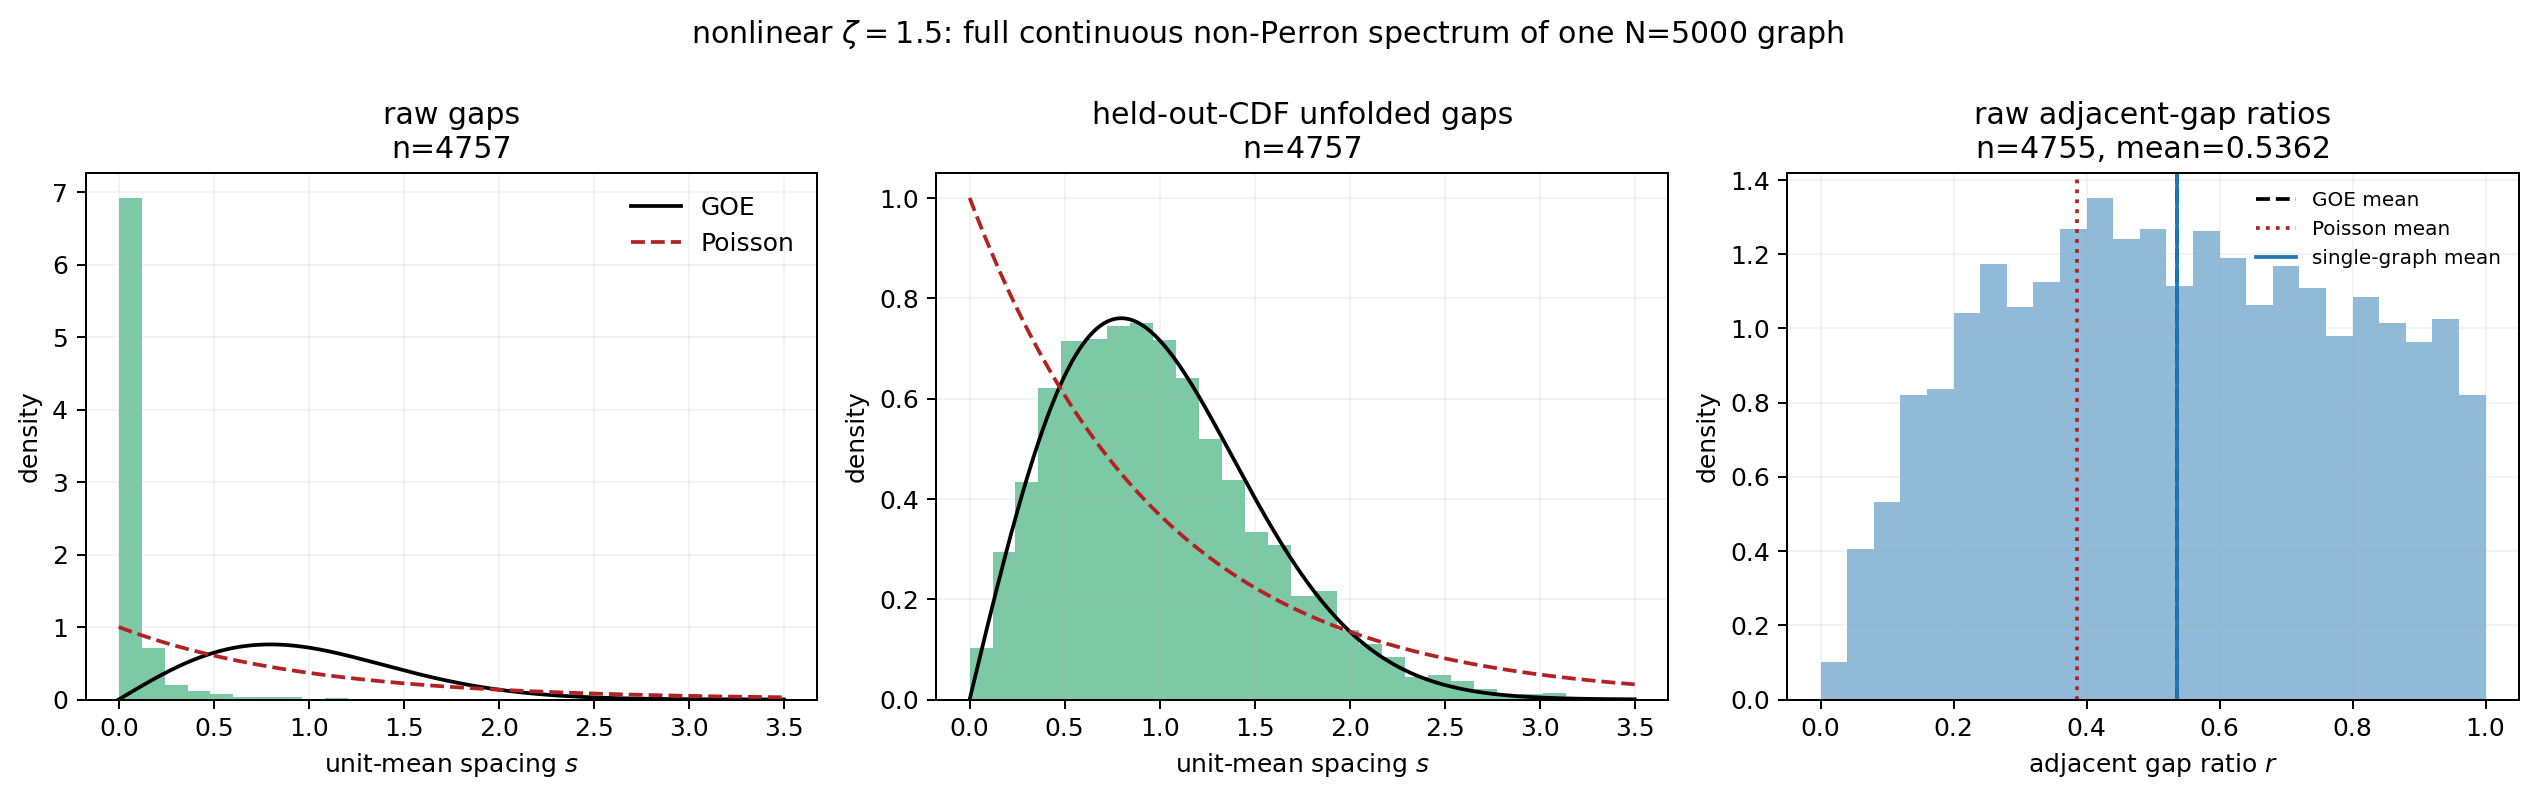
\includegraphics[width=.94\linewidth]{figures/nonlinear_zeta_1p5/histograms/single_graph_global_spacing_and_ratio.png}
\caption{Original full continuous-spectrum spacing and ratio diagnostic for nonlinear $\zeta=1.5$.}\end{figure}
\paragraph{Localization versus energy.} The continuous bulk near $E=0$ lies around $N\,\mathrm{IPR}\approx 3$--15, whereas the positive edge rises to the hundreds and occasionally near $10^3$. The positive-edge rings are cleanly separated vertically from the bulk rings, making eigenvector localization the strongest visual edge signal.
\begin{figure}[H]\centering
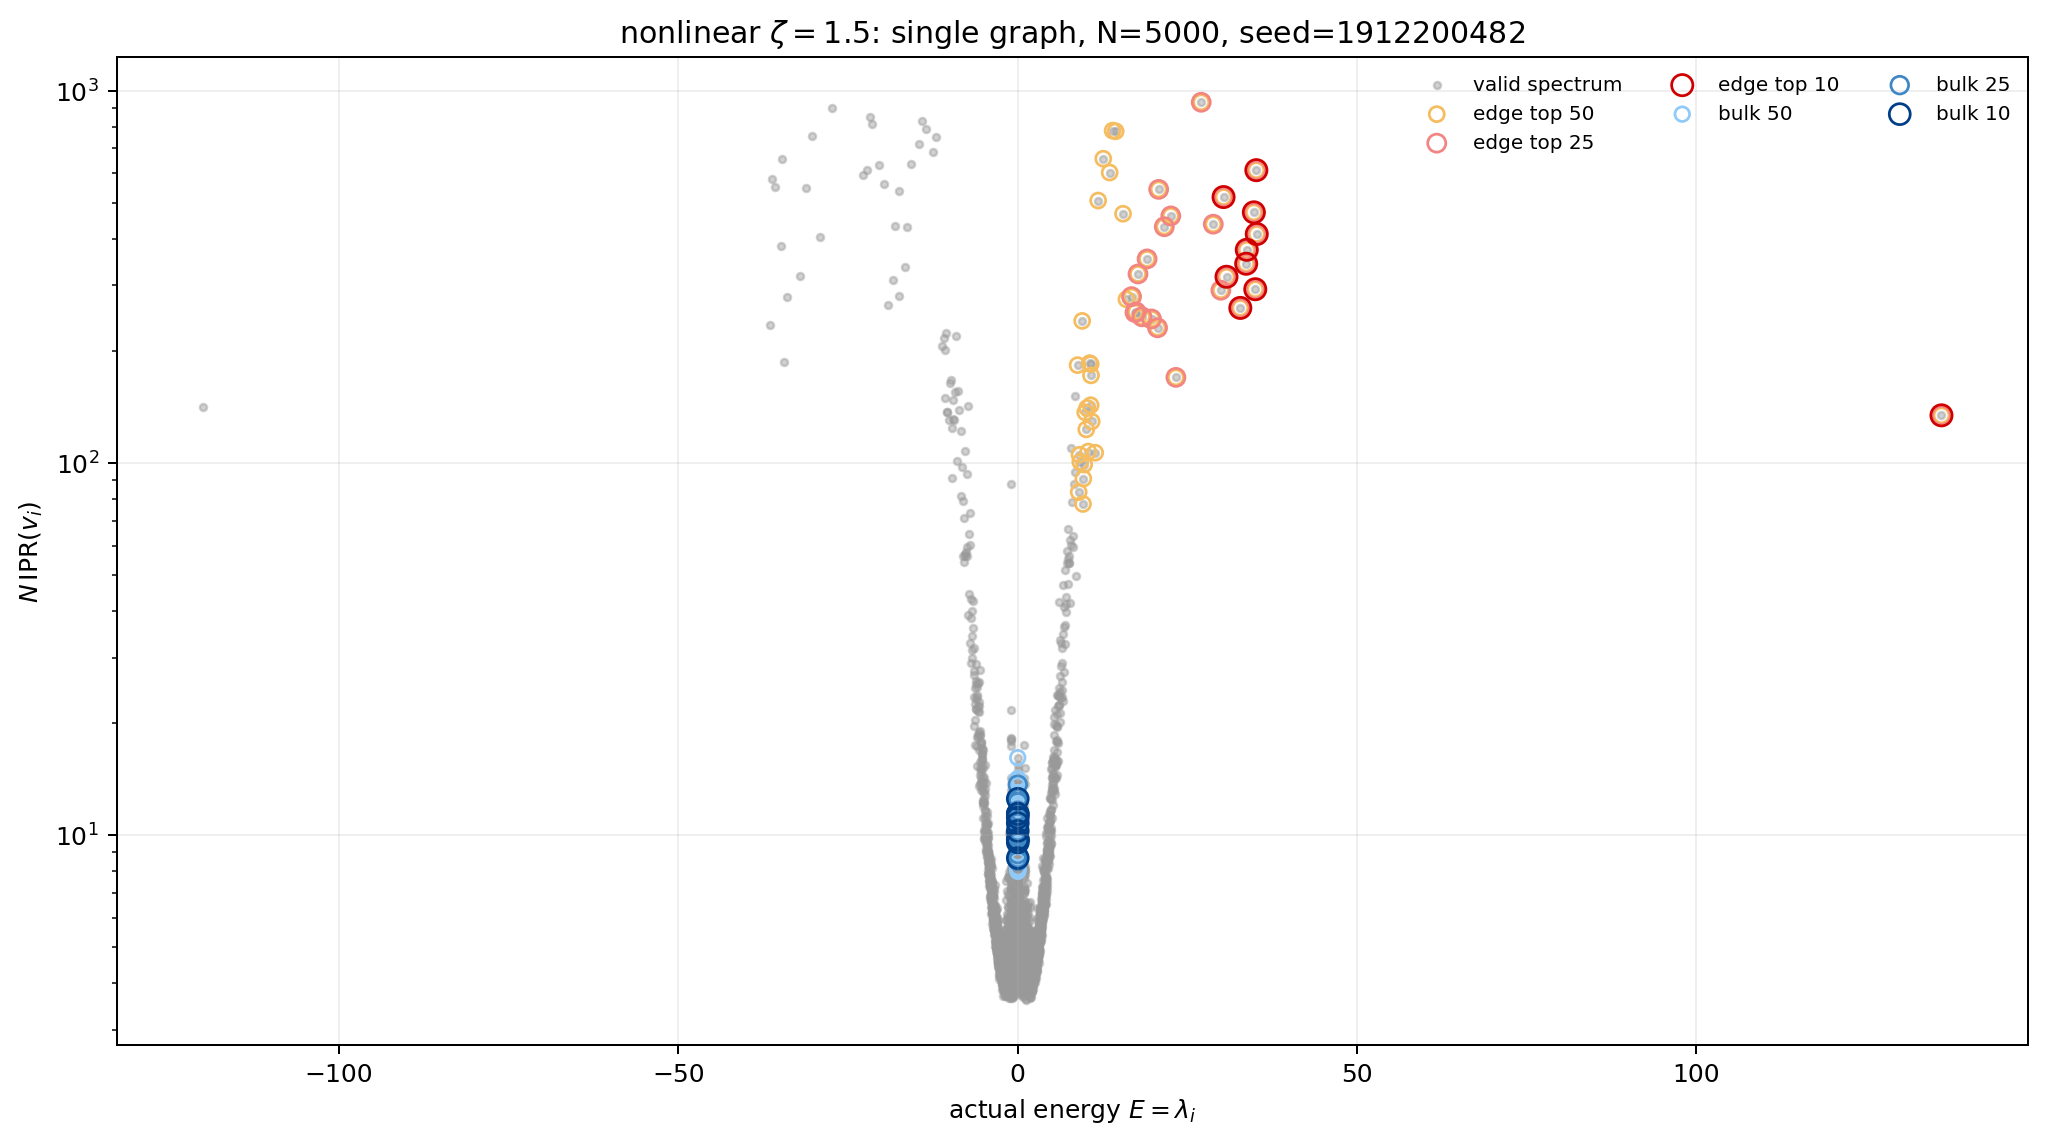
\includegraphics[width=.94\linewidth]{figures/nonlinear_zeta_1p5/energy_ipr/single_graph_localization_vs_energy.png}
\caption{Original localization-versus-energy diagnostic for nonlinear $\zeta=1.5$.}\end{figure}
\paragraph{Edge eigenpair microscope.} This is the four-panel figure highlighted in the request. The upper-left points are individual $r_i=\min(s_{i-1},s_i)/\max(s_{i-1},s_i)$ values; their large scatter is expected. Rank 2 is near zero because one adjacent gap reaches toward the isolated Perron root, which is why the strict non-Perron table begins its usable ratios at rank 3. The top-10 strict mean is near Poisson, but the top-25 and top-50 means move upward. Meanwhile $N\,\mathrm{IPR}$ stays in the hundreds through roughly rank 30 and then drops toward about 100; $M_{10}$ stays near 0.48 through roughly rank 30 before declining. The scatter panel again has no monotone $r_i$--localization relation.
\begin{figure}[H]\centering
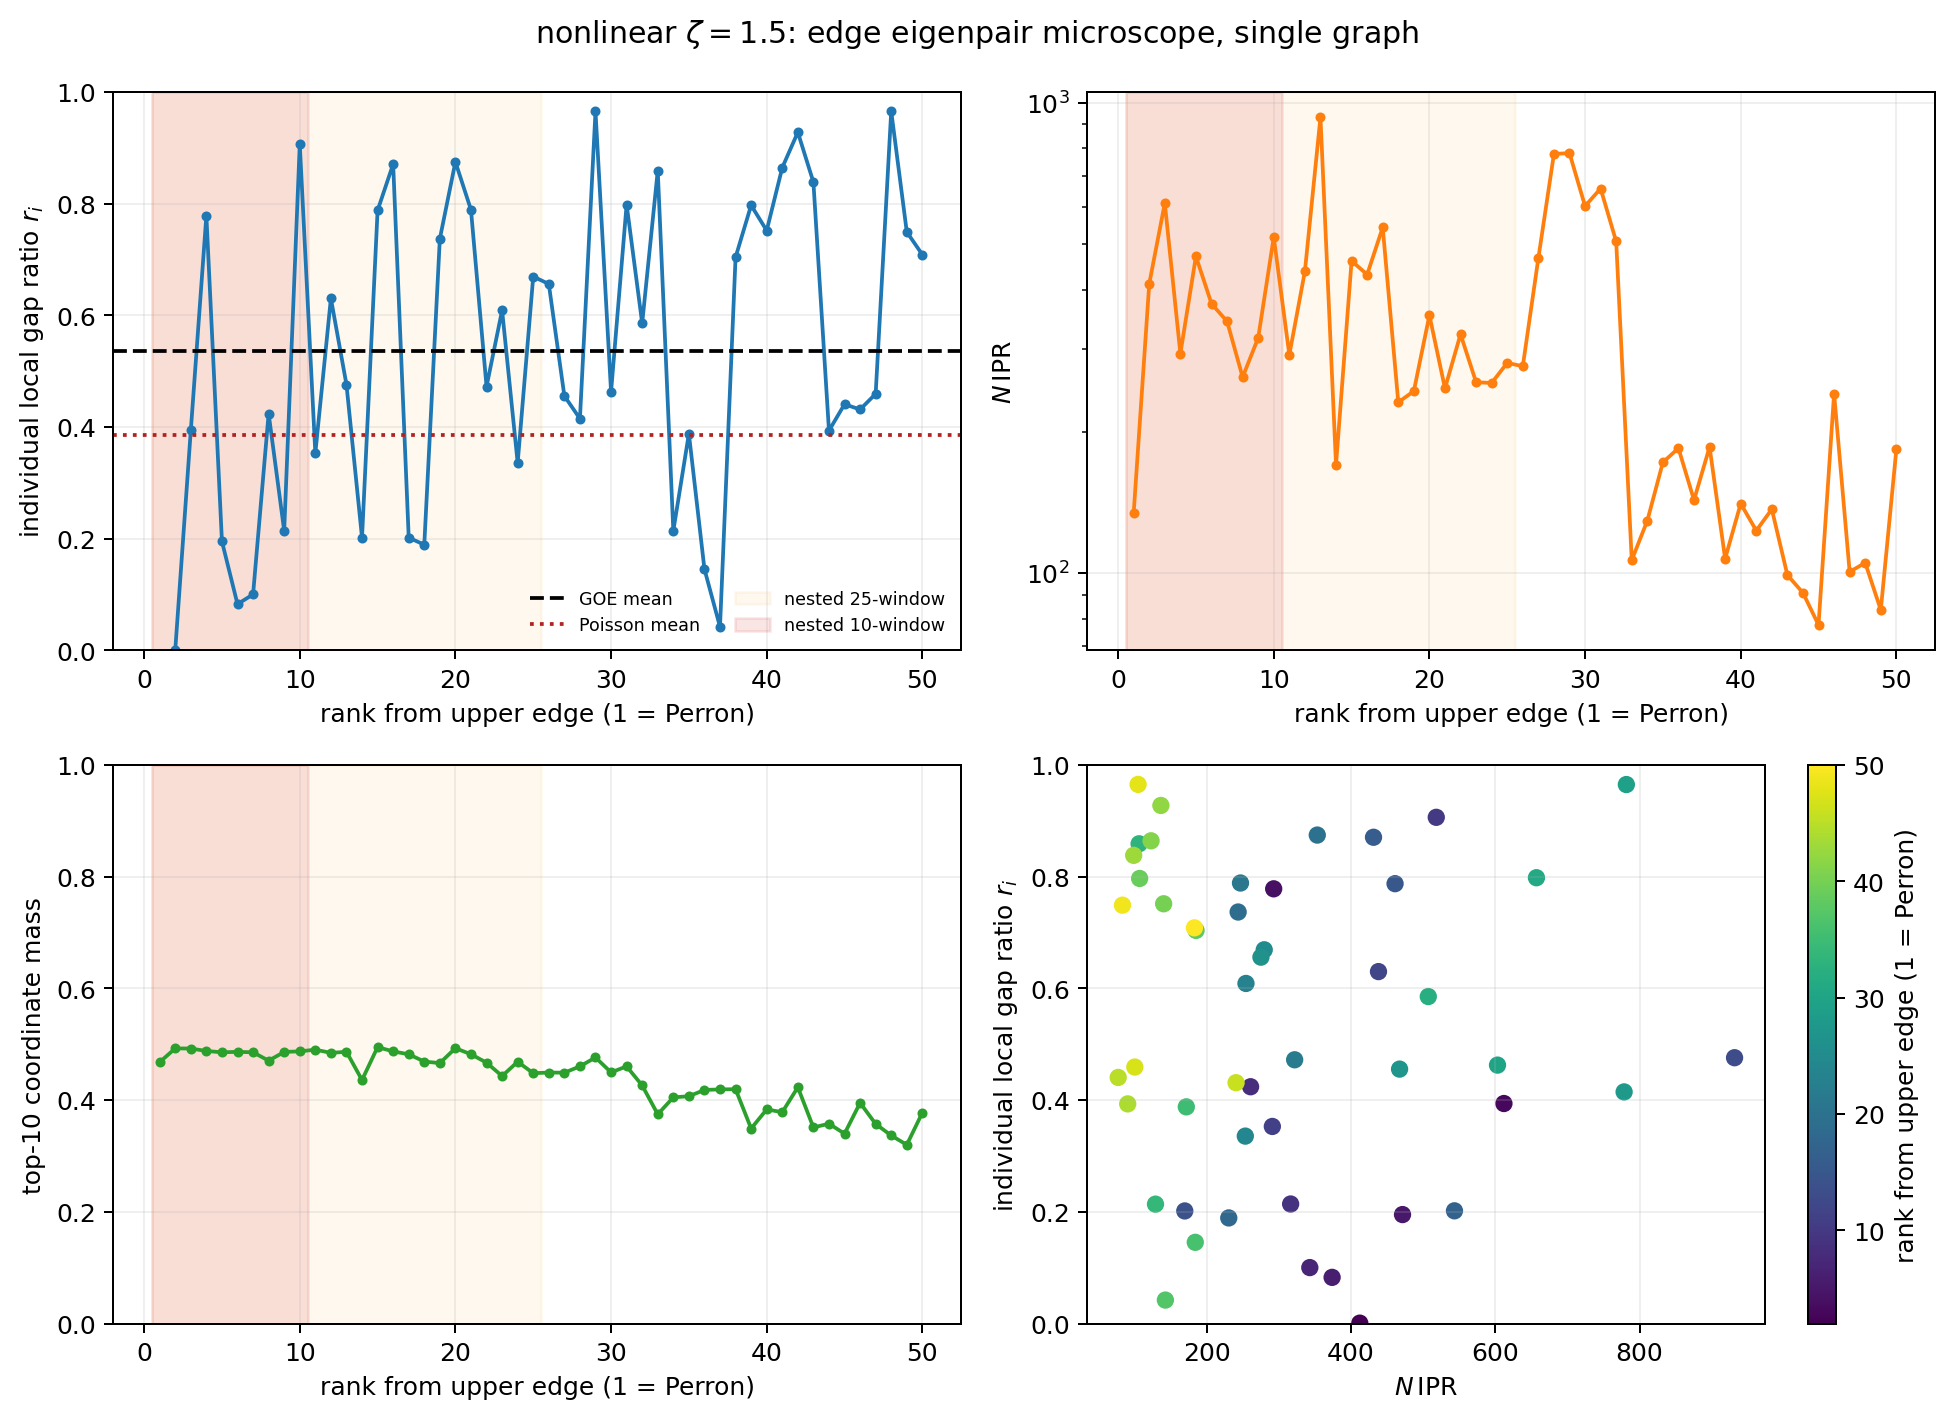
\includegraphics[width=.94\linewidth]{figures/nonlinear_zeta_1p5/edge/edge_rank_diagnostics.png}
\caption{Original four-panel edge-rank eigenpair microscope for nonlinear $\zeta=1.5$.}\end{figure}
\paragraph{Bulk eigenpair microscope.} Around the selected zero-eigenvalue-free center, $N\,\mathrm{IPR}$ remains tightly confined near 8--16 and $M_{10}$ near 0.06--0.10, despite large fluctuations in individual $r_i$. This is the cleanest example of why the bulk can be extended even when a short sequence of ratios happens to contain both Poisson-like and GOE-like values.
\begin{figure}[H]\centering
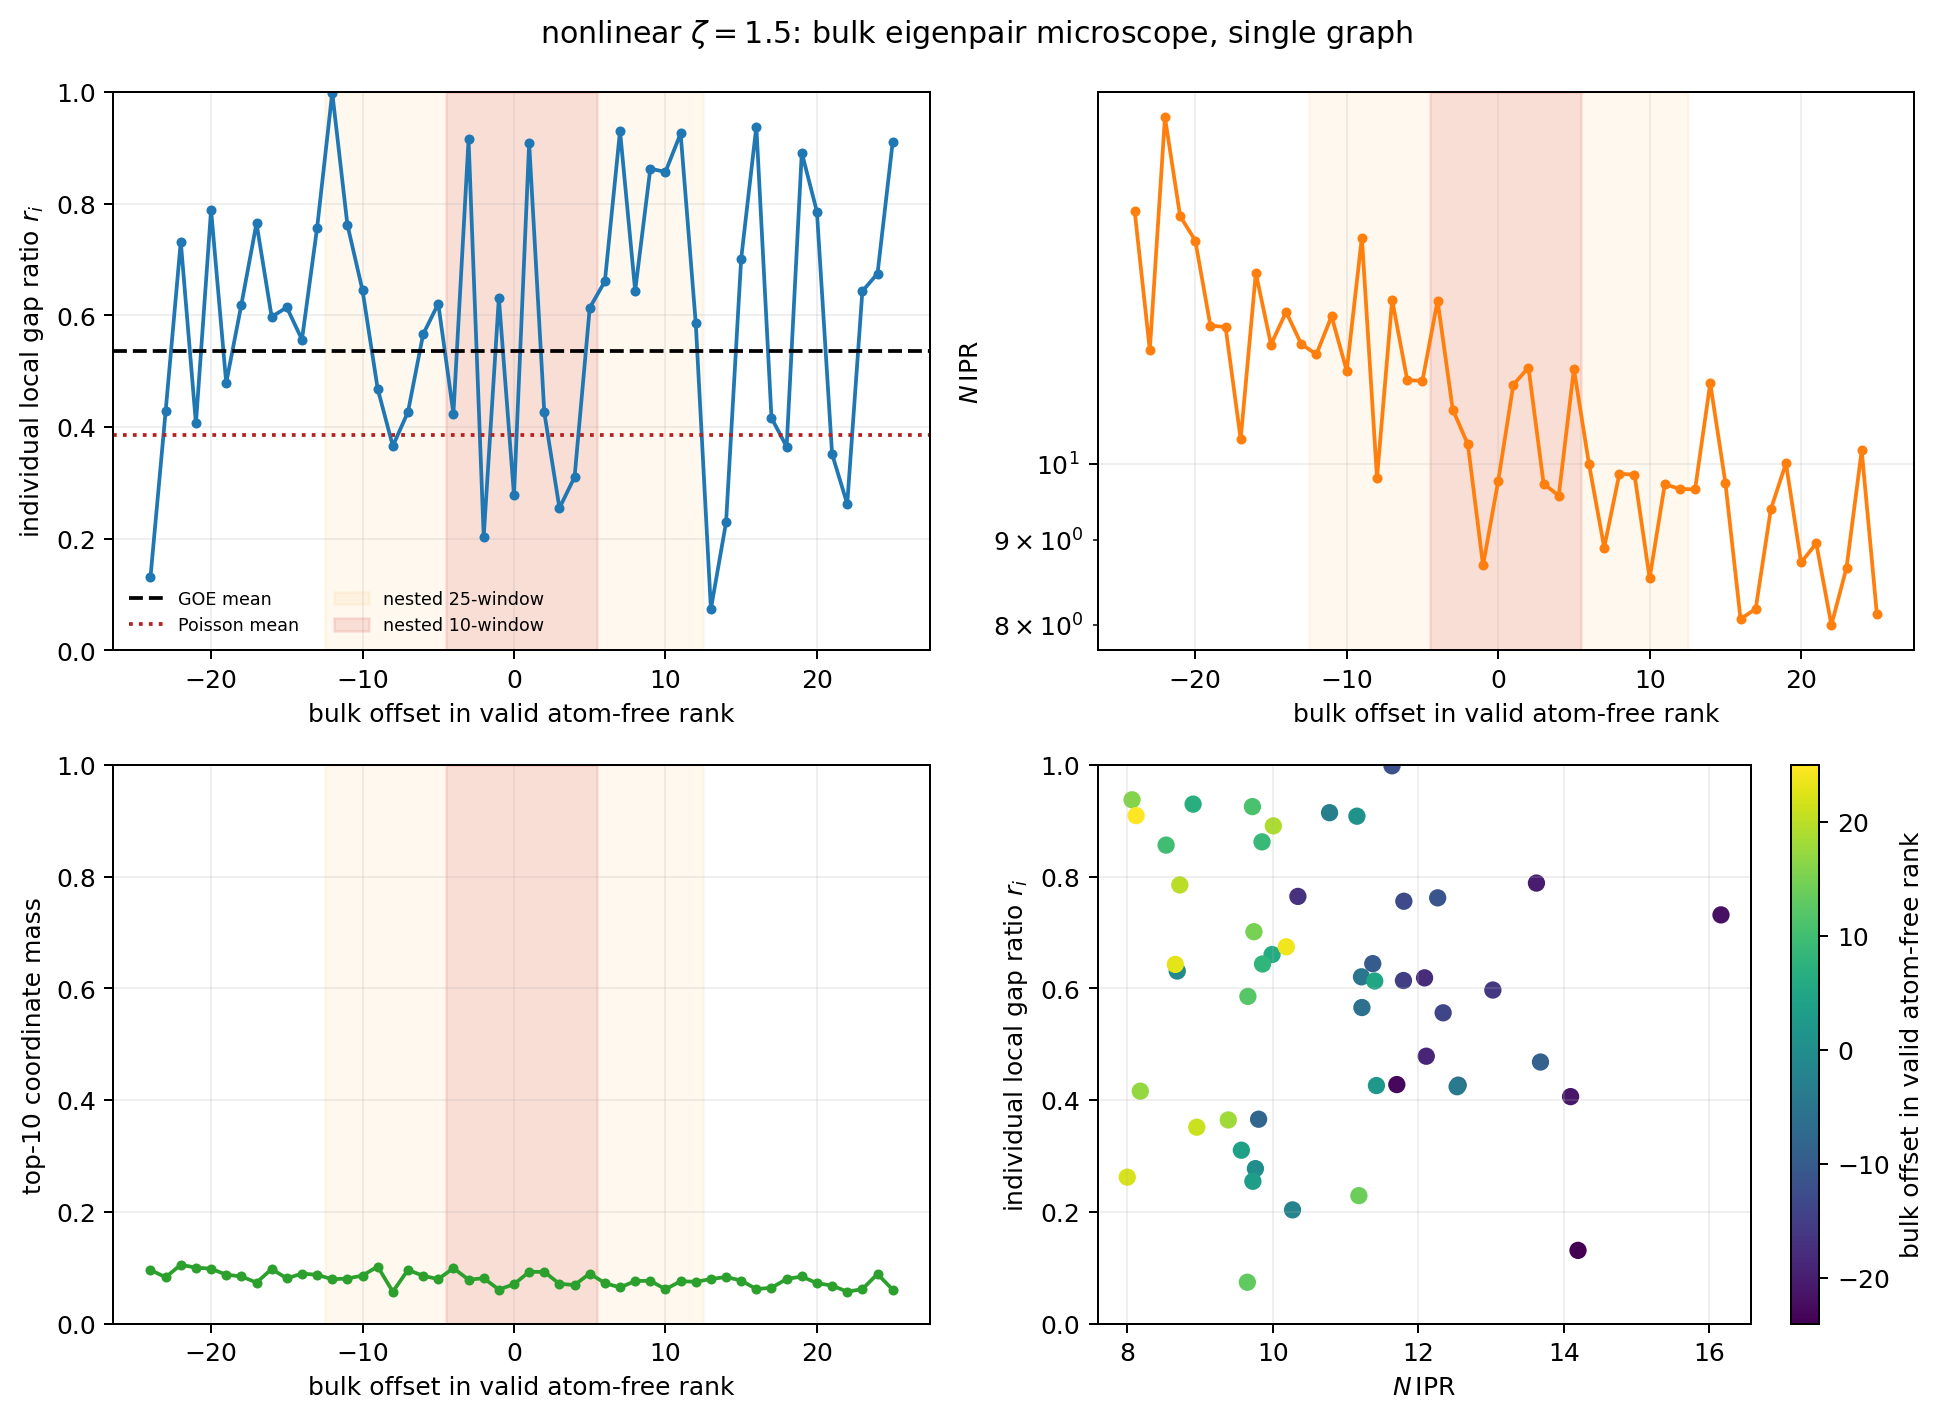
\includegraphics[width=.94\linewidth]{figures/nonlinear_zeta_1p5/bulk/bulk_offset_diagnostics.png}
\caption{Original four-panel centered bulk-offset eigenpair microscope for nonlinear $\zeta=1.5$.}\end{figure}
\paragraph{Direct edge-versus-bulk comparison.} The edge and bulk distributions are almost disjoint in $N\,\mathrm{IPR}$ and $M_{10}$. Edge top-mass vertices also have much higher degree, form substantially denser induced subgraphs, and have shorter full-graph paths. The bulk induced density is exactly zero for these displayed supports, while the edge density is often large; this is a structural localization signature independent of the ambiguous ratio average.
\begin{figure}[H]\centering
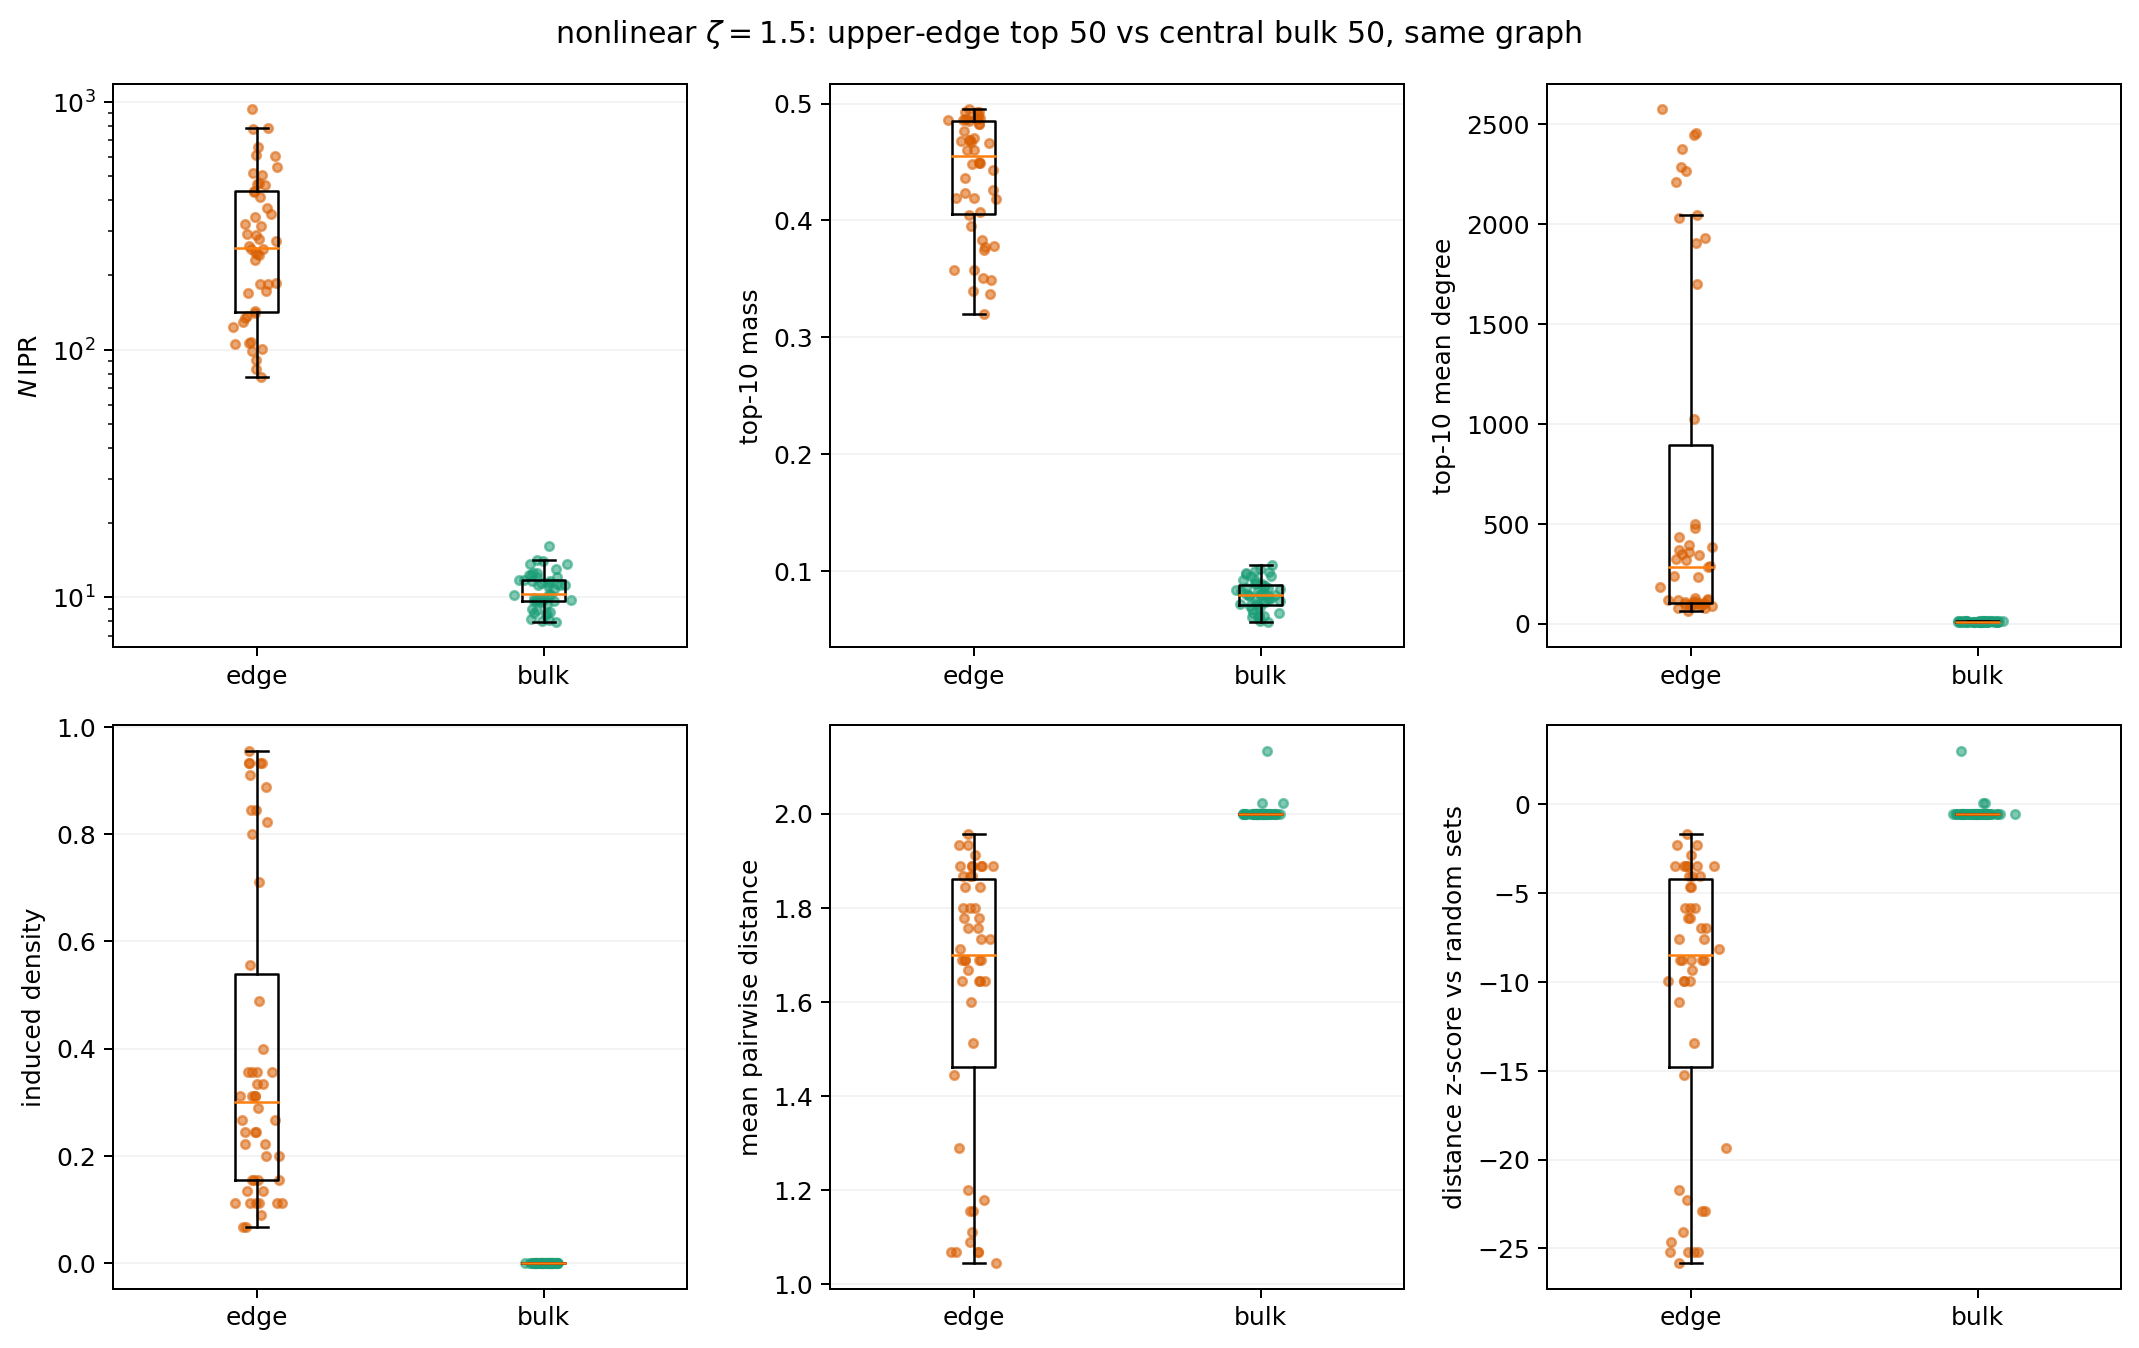
\includegraphics[width=.94\linewidth]{figures/nonlinear_zeta_1p5/edge_vs_bulk/edge_vs_bulk_comparison.png}
\caption{Original direct edge-versus-bulk comparison for nonlinear $\zeta=1.5$.}\end{figure}
\subsection{affine $\alpha=2.0$}
\paragraph{Eigenvalue density.} This model has no repeated zero eigenvalues in the stored graph: 4,999 continuous non-Perron levels remain. Its broad, smooth density makes it the clean control for separating edge localization from zero-eigenvalue or rank-deficiency effects.
\begin{figure}[H]\centering
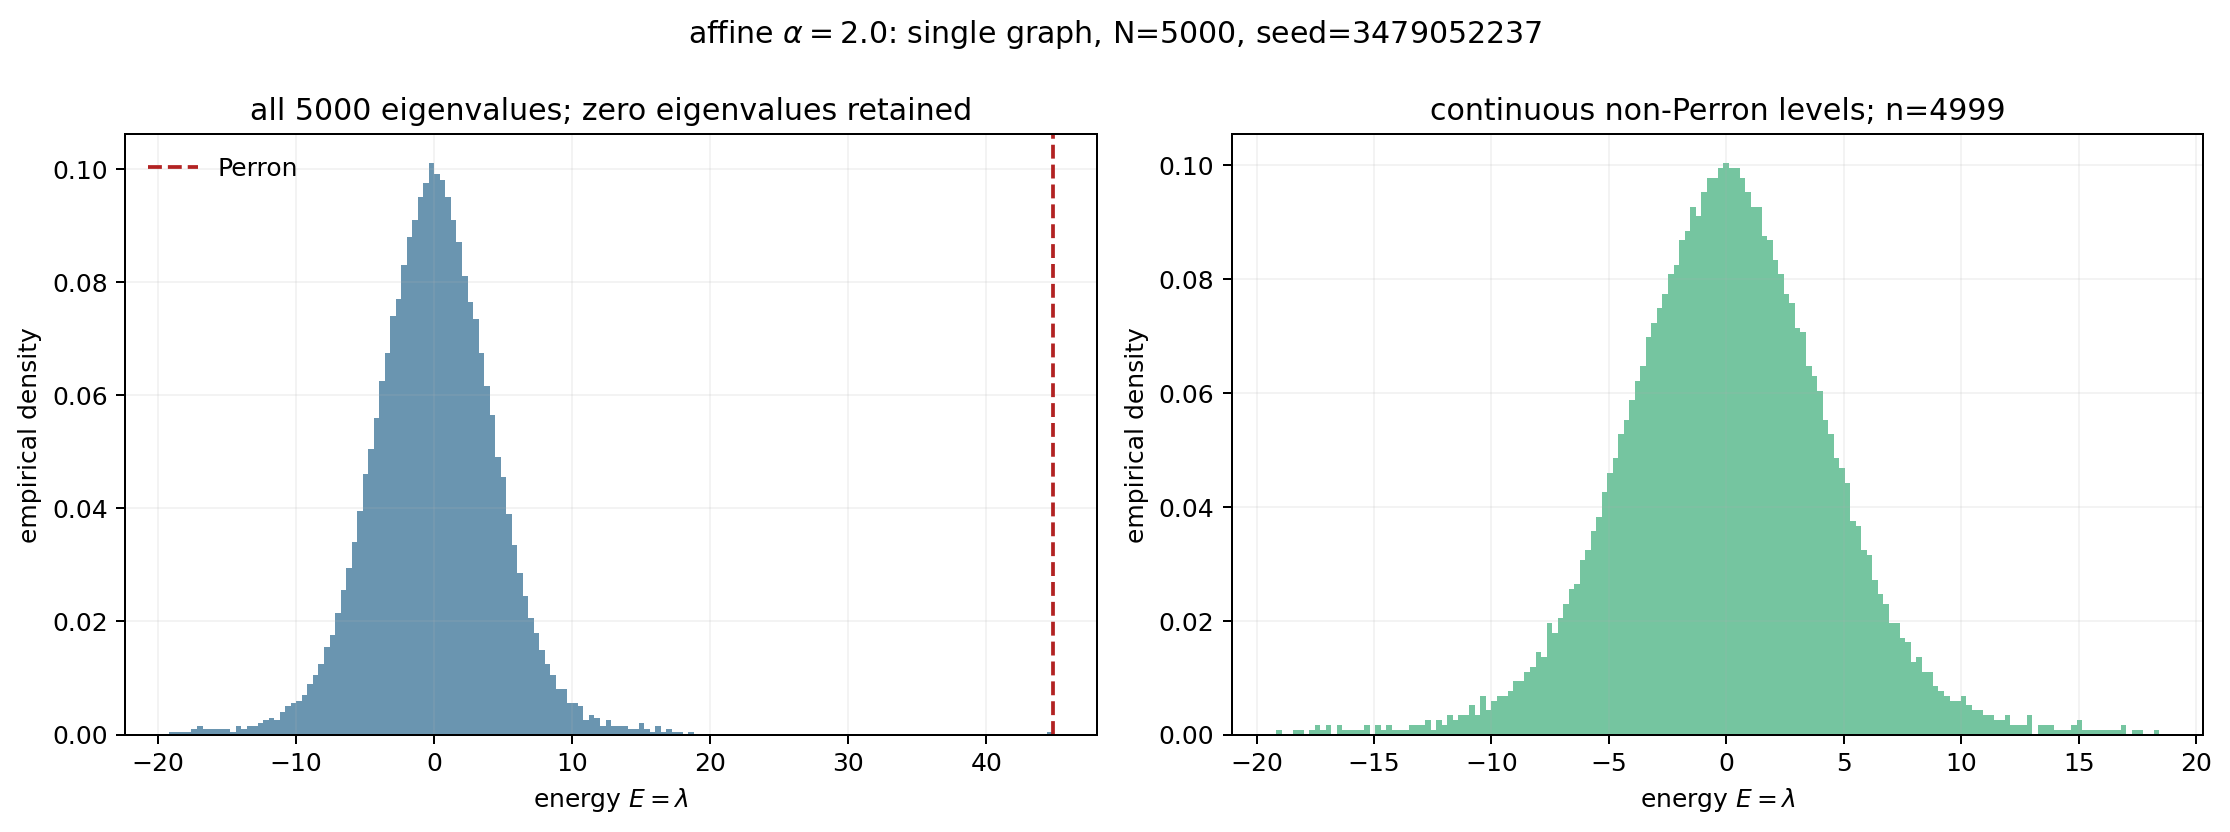
\includegraphics[width=.94\linewidth]{figures/affine_alpha_2p0/spectrum/single_graph_eigenvalue_density.png}
\caption{Original single-graph eigenvalue-density diagnostic for affine $\alpha=2.0$.}\end{figure}
\paragraph{Raw and unfolded local spacing.} The unfolded interior histograms track the GOE reference reasonably well, while extreme-edge panels have far fewer gaps and visible discreteness. The full-spectrum ratio mean is about 0.525, again close to GOE. Thus localization at this edge does not require an overall Poisson gap-ratio law in this single graph.
\begin{figure}[H]\centering
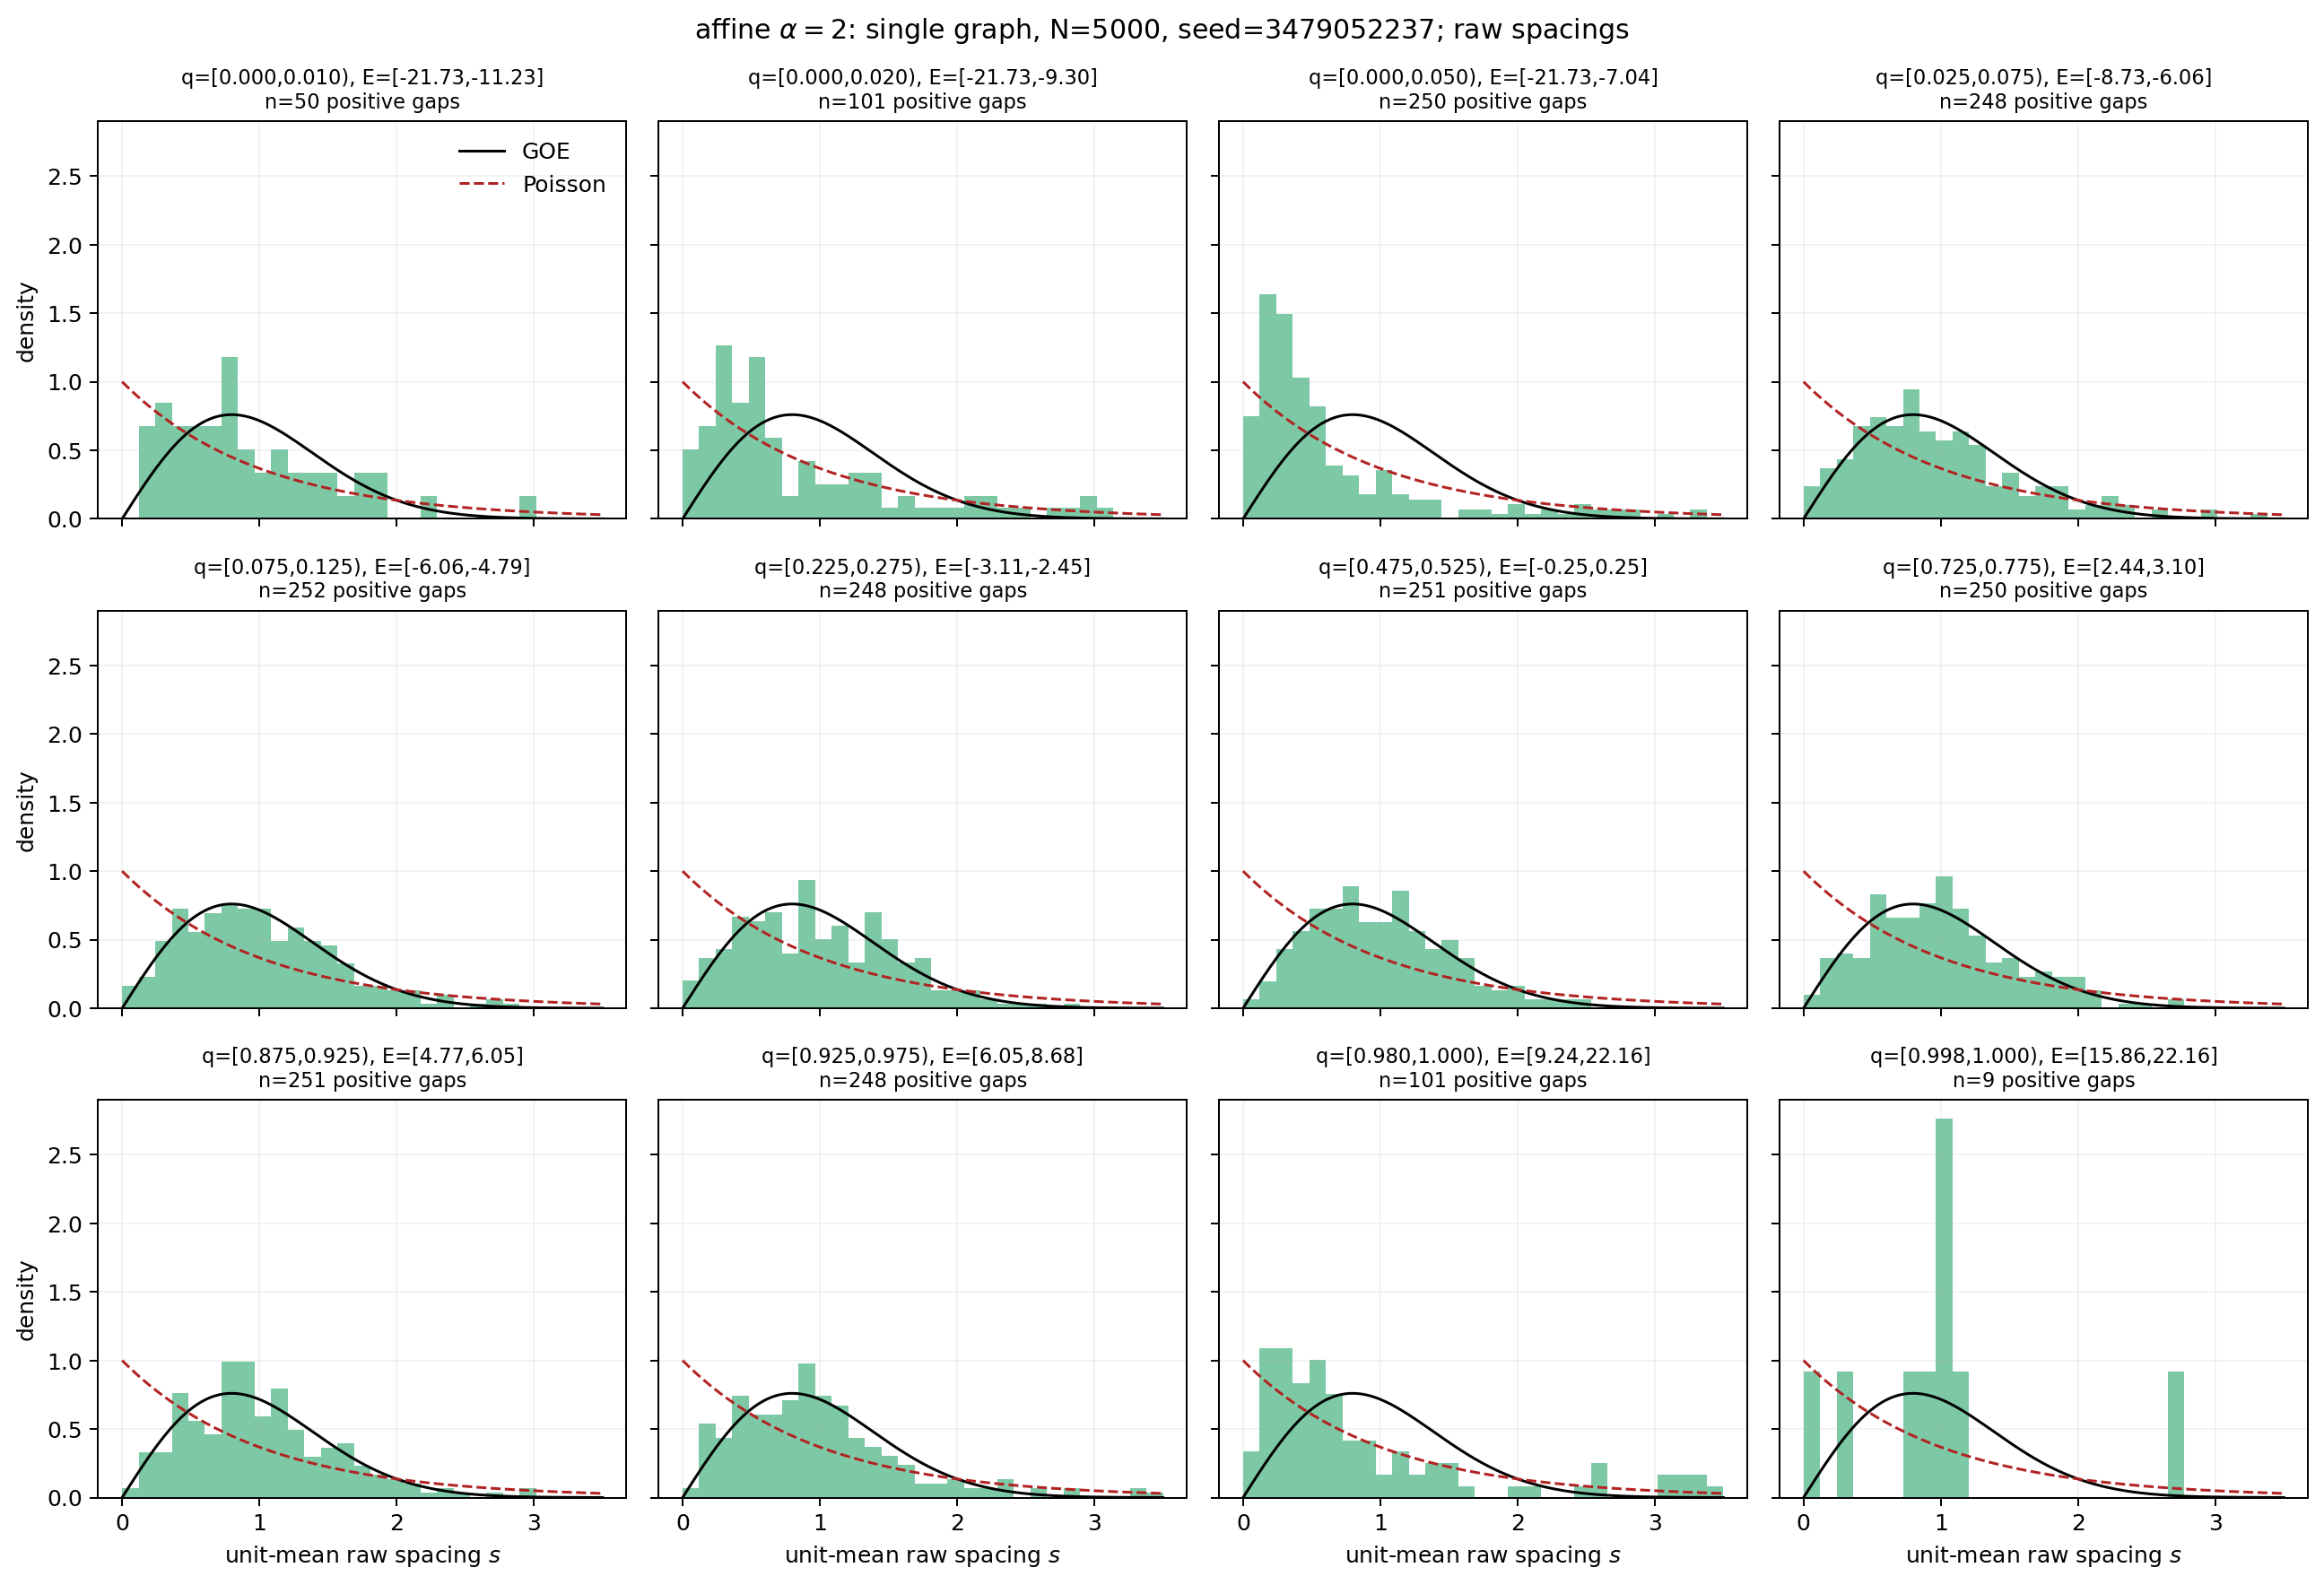
\includegraphics[width=.94\linewidth]{figures/affine_alpha_2p0/histograms/single_graph_local_raw_spacing_histograms.png}
\caption{Original local raw-spacing histograms for affine $\alpha=2.0$.}\end{figure}
\begin{figure}[H]\centering
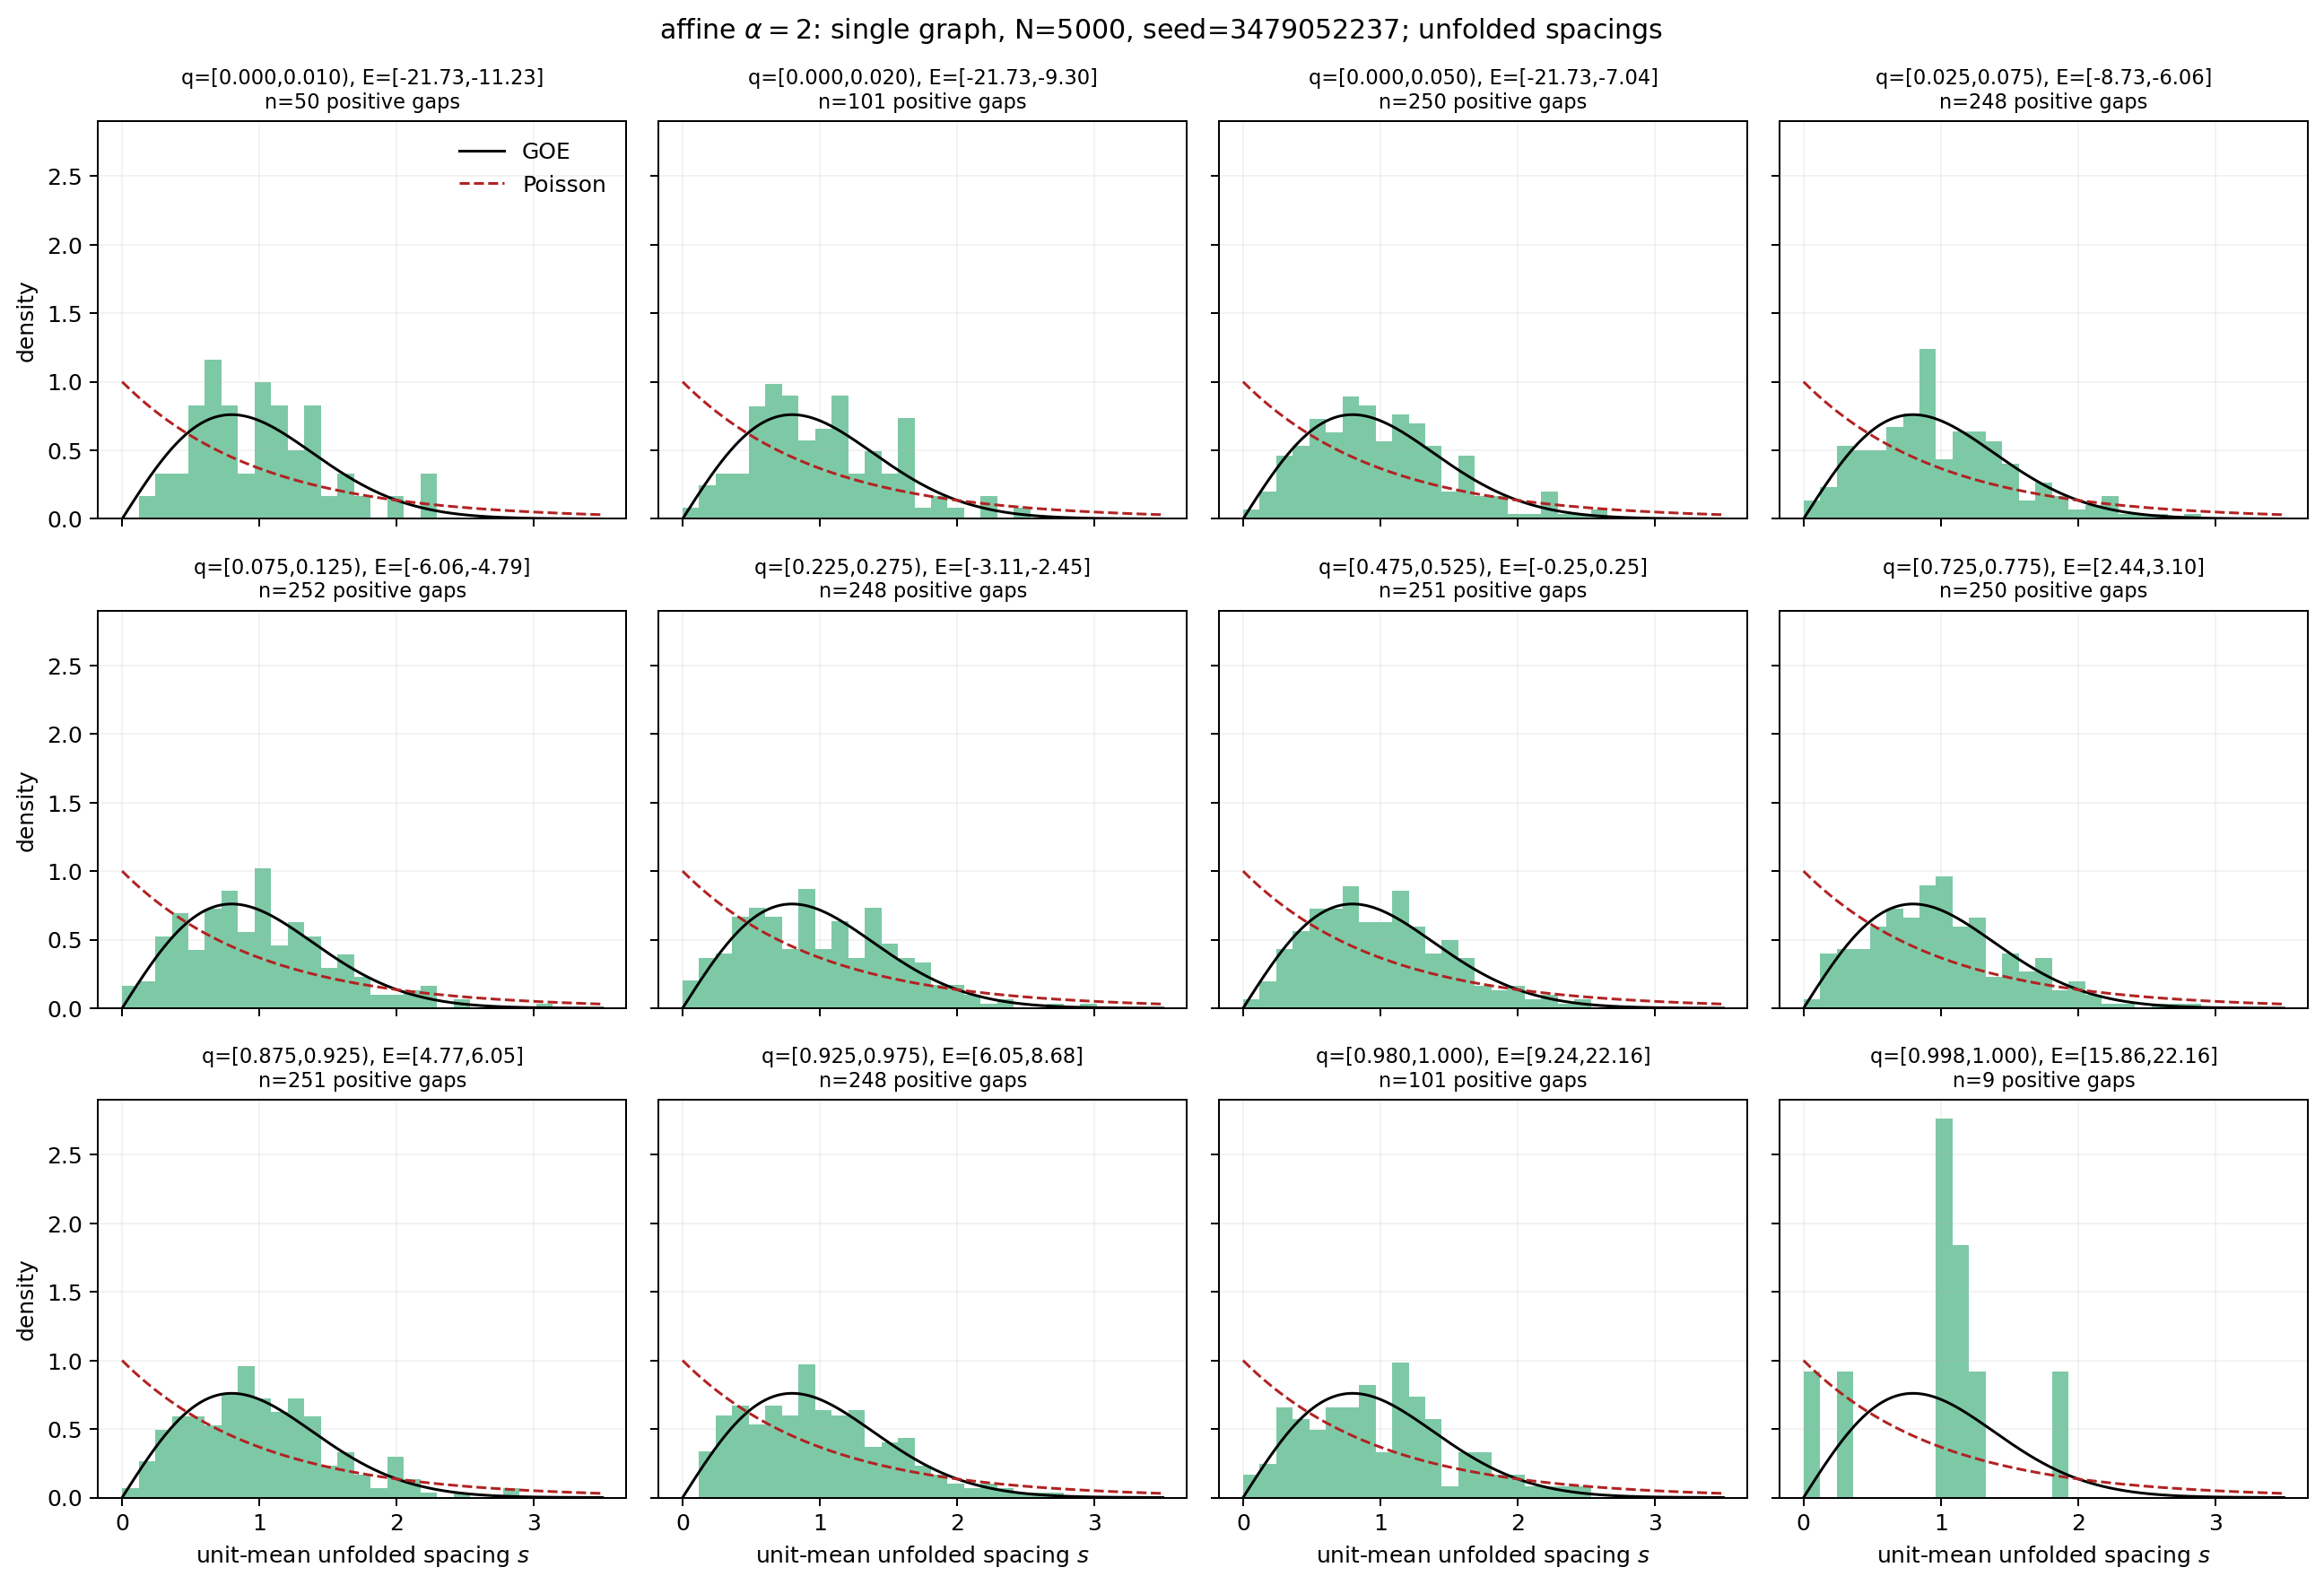
\includegraphics[width=.94\linewidth]{figures/affine_alpha_2p0/histograms/single_graph_local_unfolded_spacing_histograms.png}
\caption{Original local unfolded-spacing histograms for affine $\alpha=2.0$.}\end{figure}
\begin{figure}[H]\centering
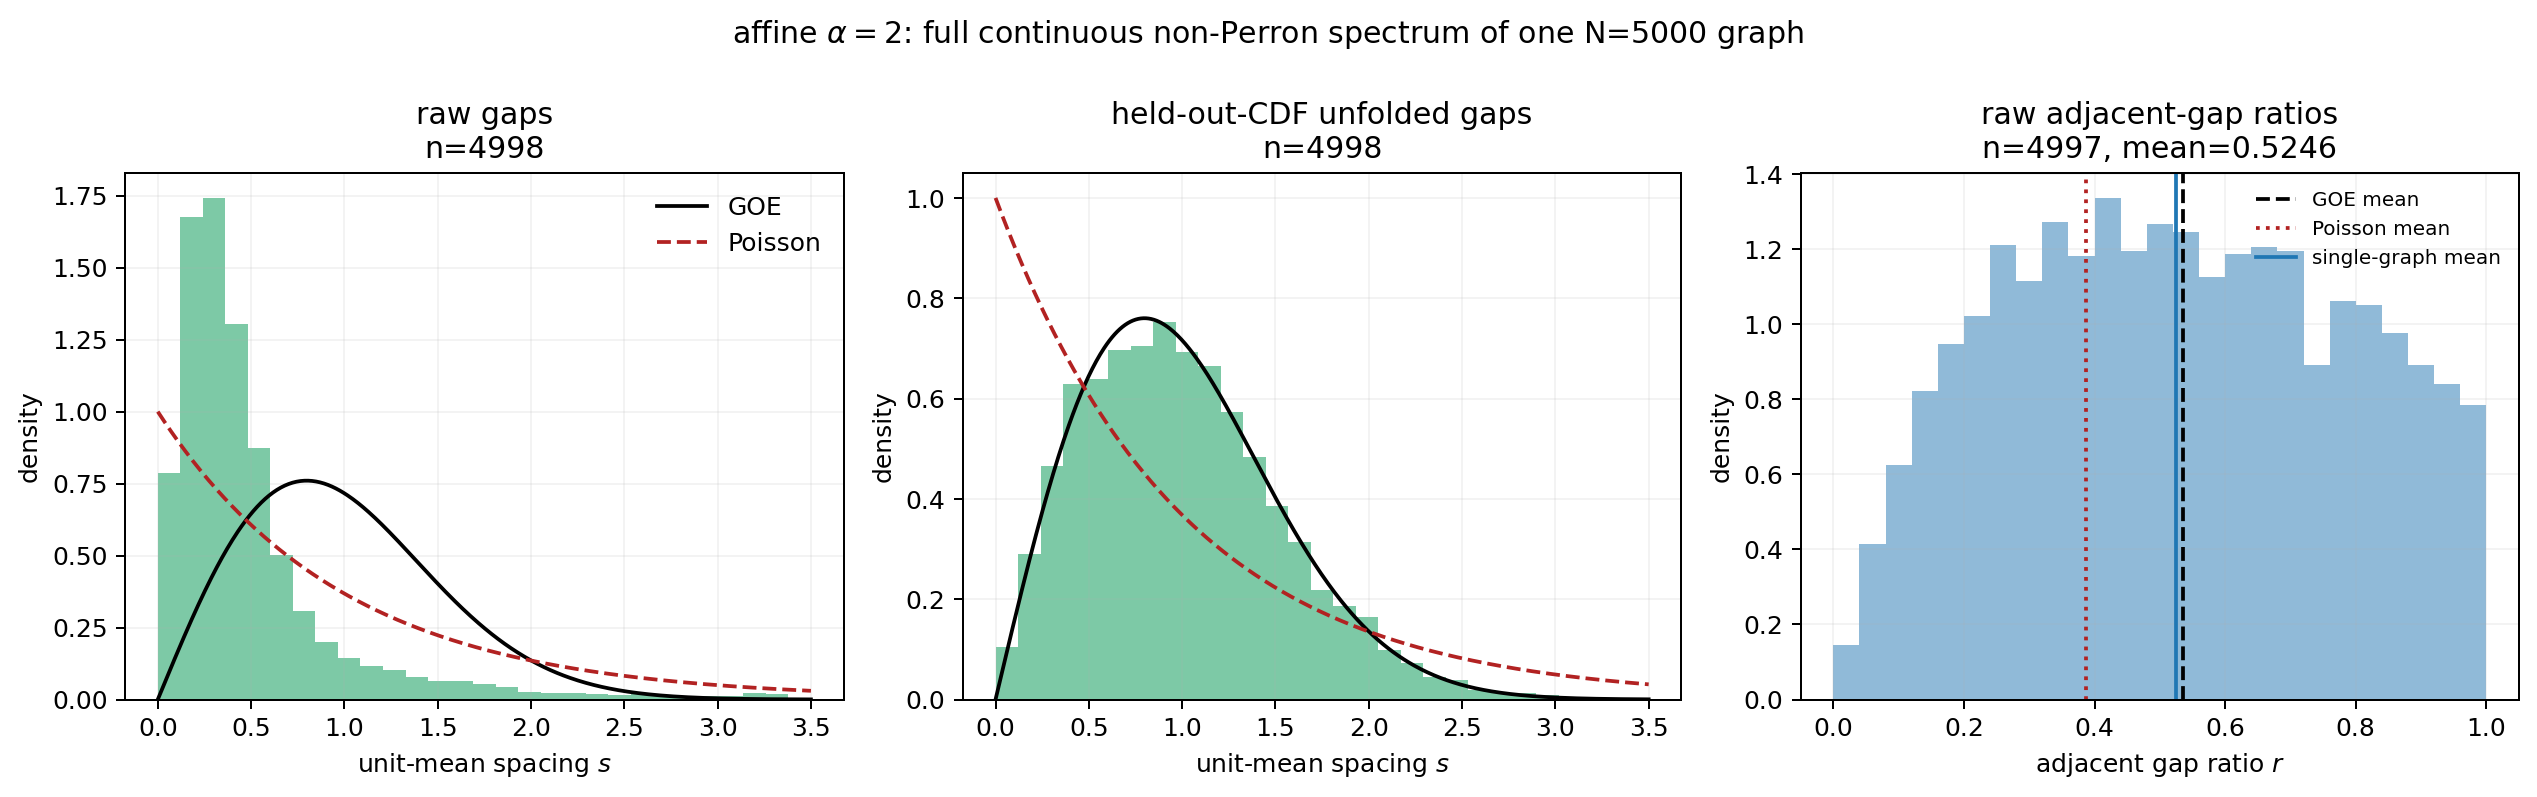
\includegraphics[width=.94\linewidth]{figures/affine_alpha_2p0/histograms/single_graph_global_spacing_and_ratio.png}
\caption{Original full continuous-spectrum spacing and ratio diagnostic for affine $\alpha=2.0$.}\end{figure}
\paragraph{Localization versus energy.} The $N\,\mathrm{IPR}$ bowl is smooth and symmetric apart from the isolated Perron point: values are near 4 in the bulk and rise into the tens or hundreds toward the tails. This provides the clearest visual mobility-edge-like crossover of the three graphs, although one realization cannot locate a sharp transition.
\begin{figure}[H]\centering
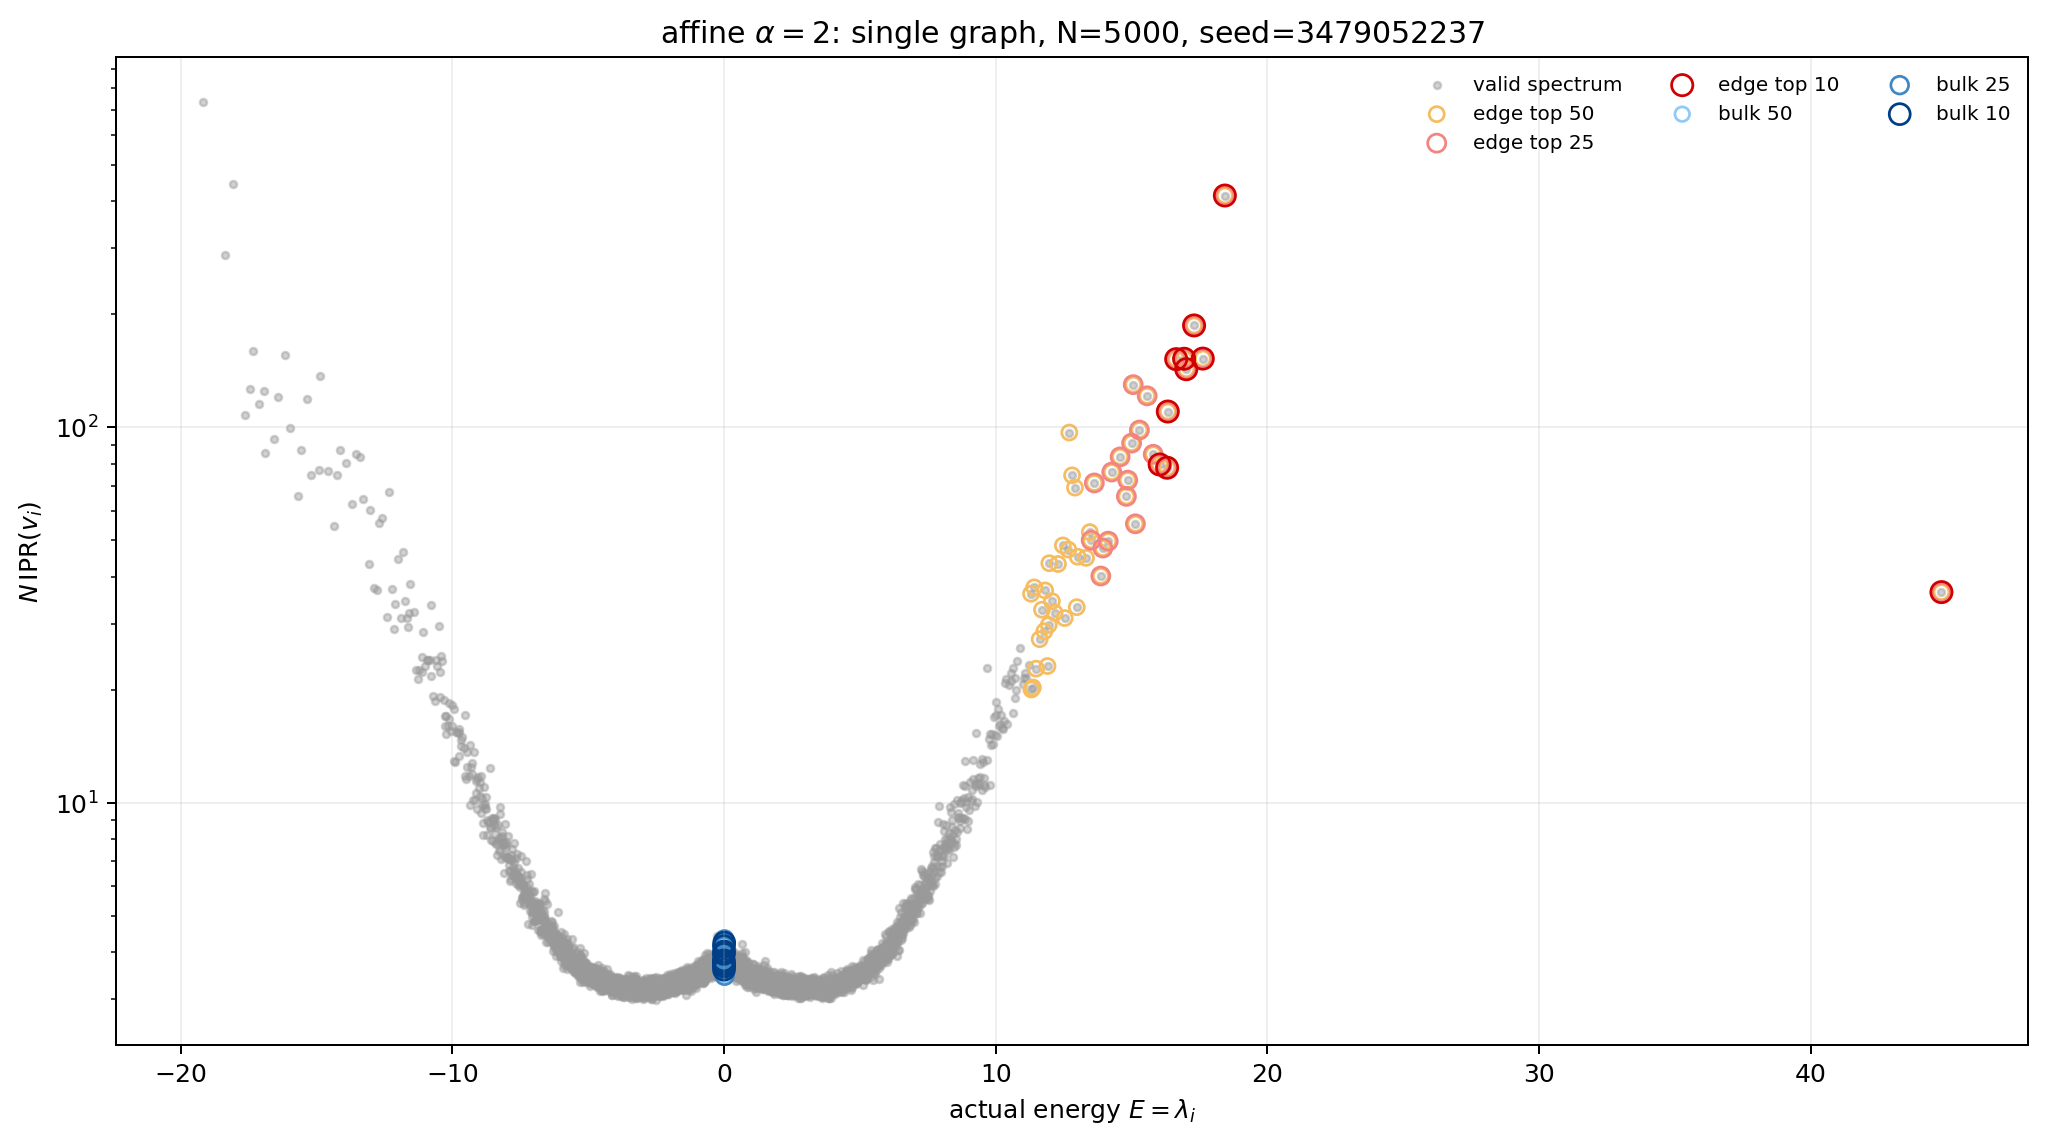
\includegraphics[width=.94\linewidth]{figures/affine_alpha_2p0/energy_ipr/single_graph_localization_vs_energy.png}
\caption{Original localization-versus-energy diagnostic for affine $\alpha=2.0$.}\end{figure}
\paragraph{Edge eigenpair microscope.} The upper-right and lower-left panels decline fairly steadily with rank: $N\,\mathrm{IPR}$ falls from hundreds to a few tens, and $M_{10}$ falls from roughly 0.4 to 0.15--0.2. Individual ratios still jump between small and large values, and the scatter plot shows no single-valued relation between $r_i$ and $N\,\mathrm{IPR}$. The localization crossover is much clearer than any crossover in $r_i$.
\begin{figure}[H]\centering
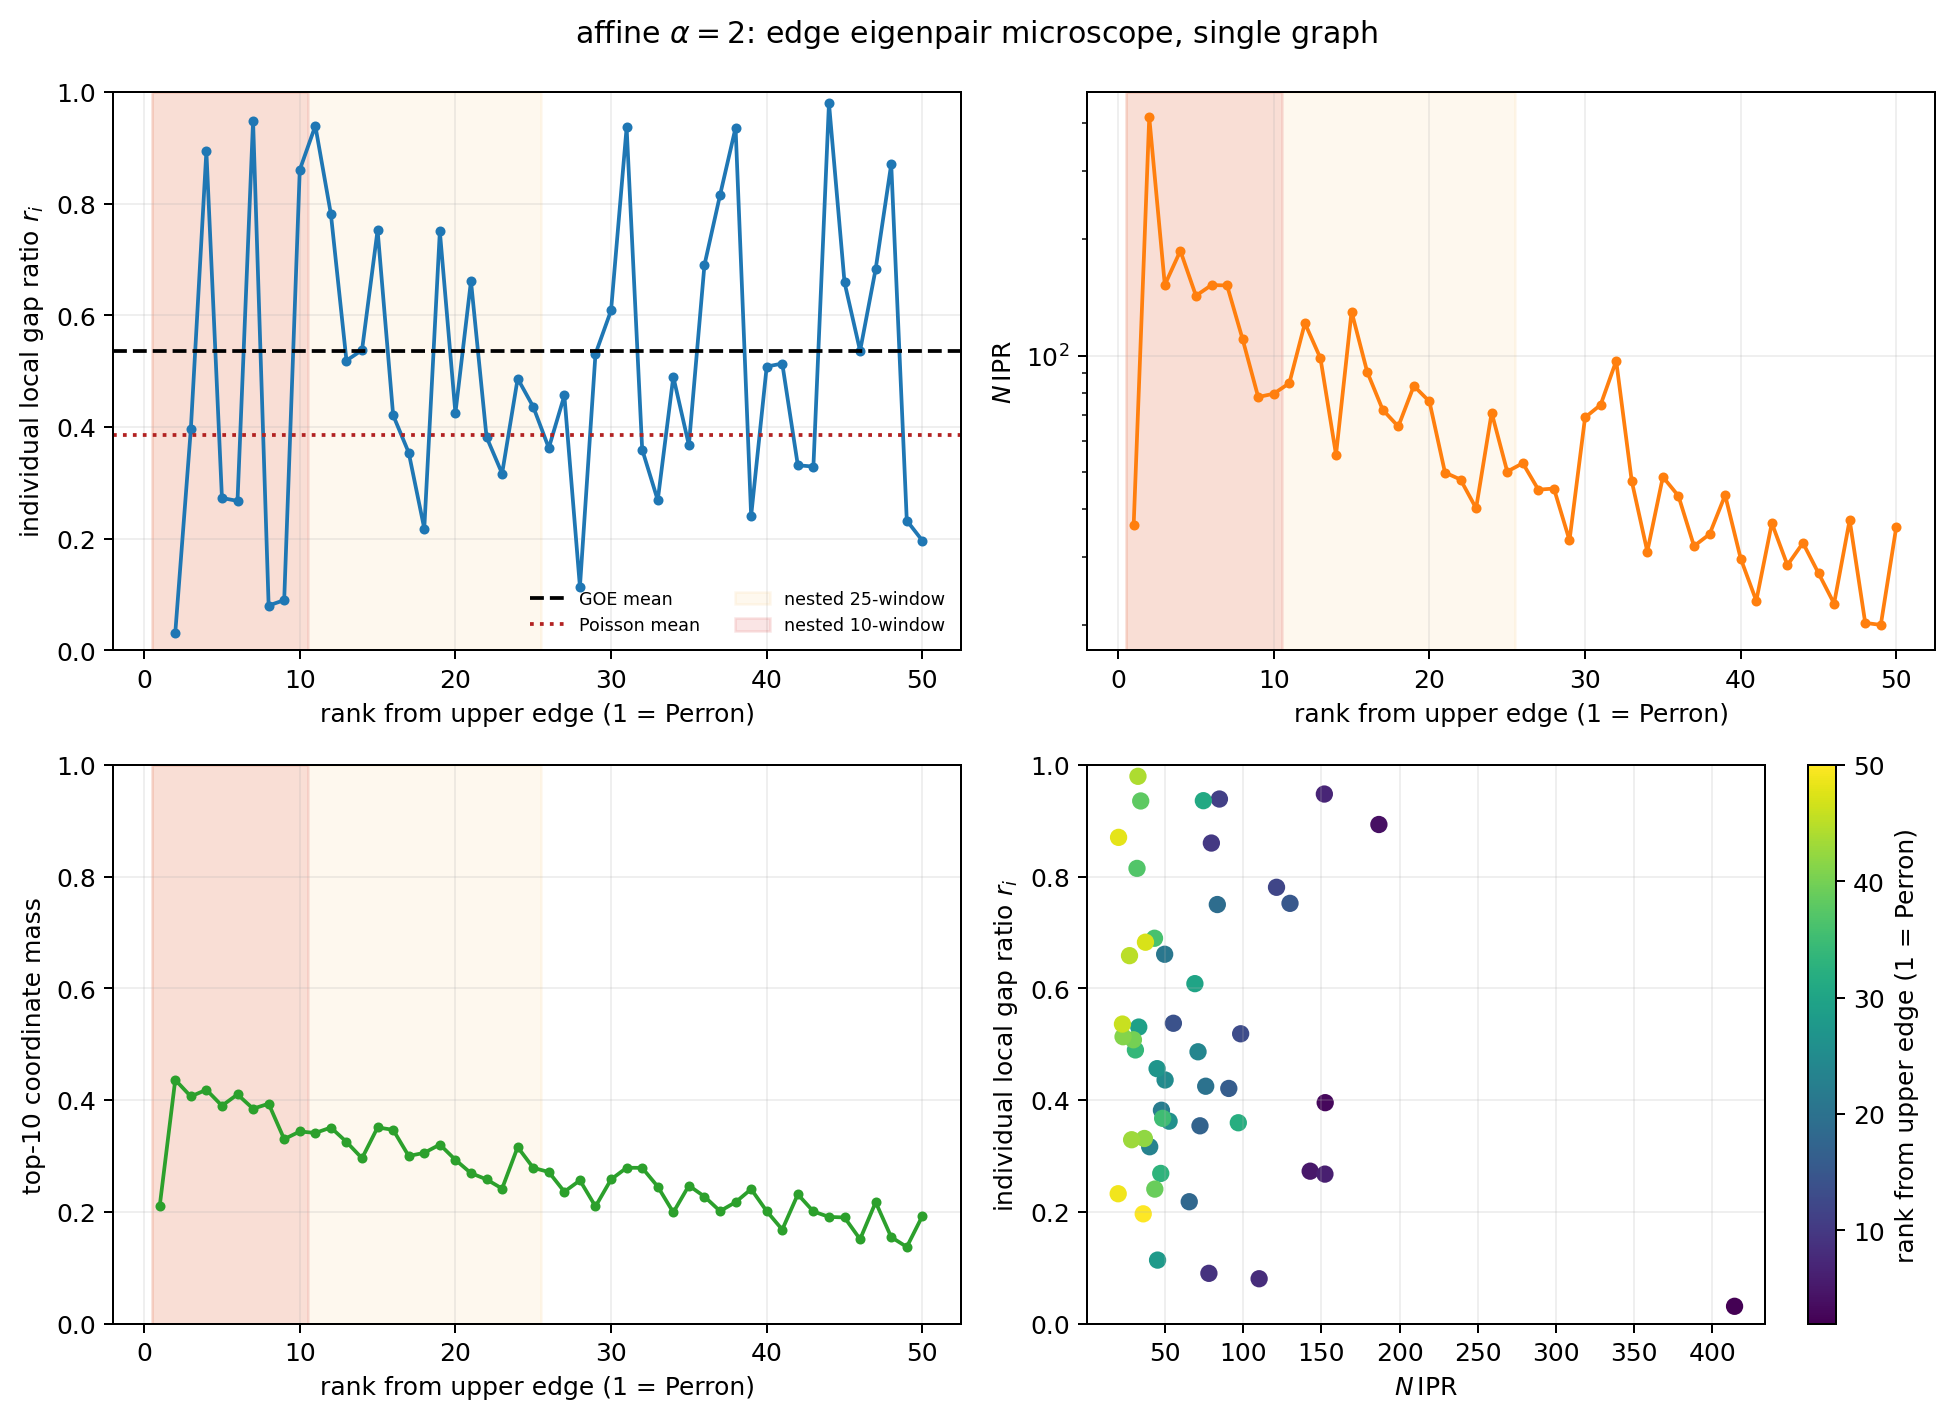
\includegraphics[width=.94\linewidth]{figures/affine_alpha_2p0/edge/edge_rank_diagnostics.png}
\caption{Original four-panel edge-rank eigenpair microscope for affine $\alpha=2.0$.}\end{figure}
\paragraph{Bulk eigenpair microscope.} The bulk localization panels are nearly flat: $N\,\mathrm{IPR}$ stays around 3.5--4.3 and $M_{10}$ around 0.03. Pointwise gap ratios remain noisy, but their fluctuations occur on an eigenvector background that is uniformly extended relative to the edge.
\begin{figure}[H]\centering
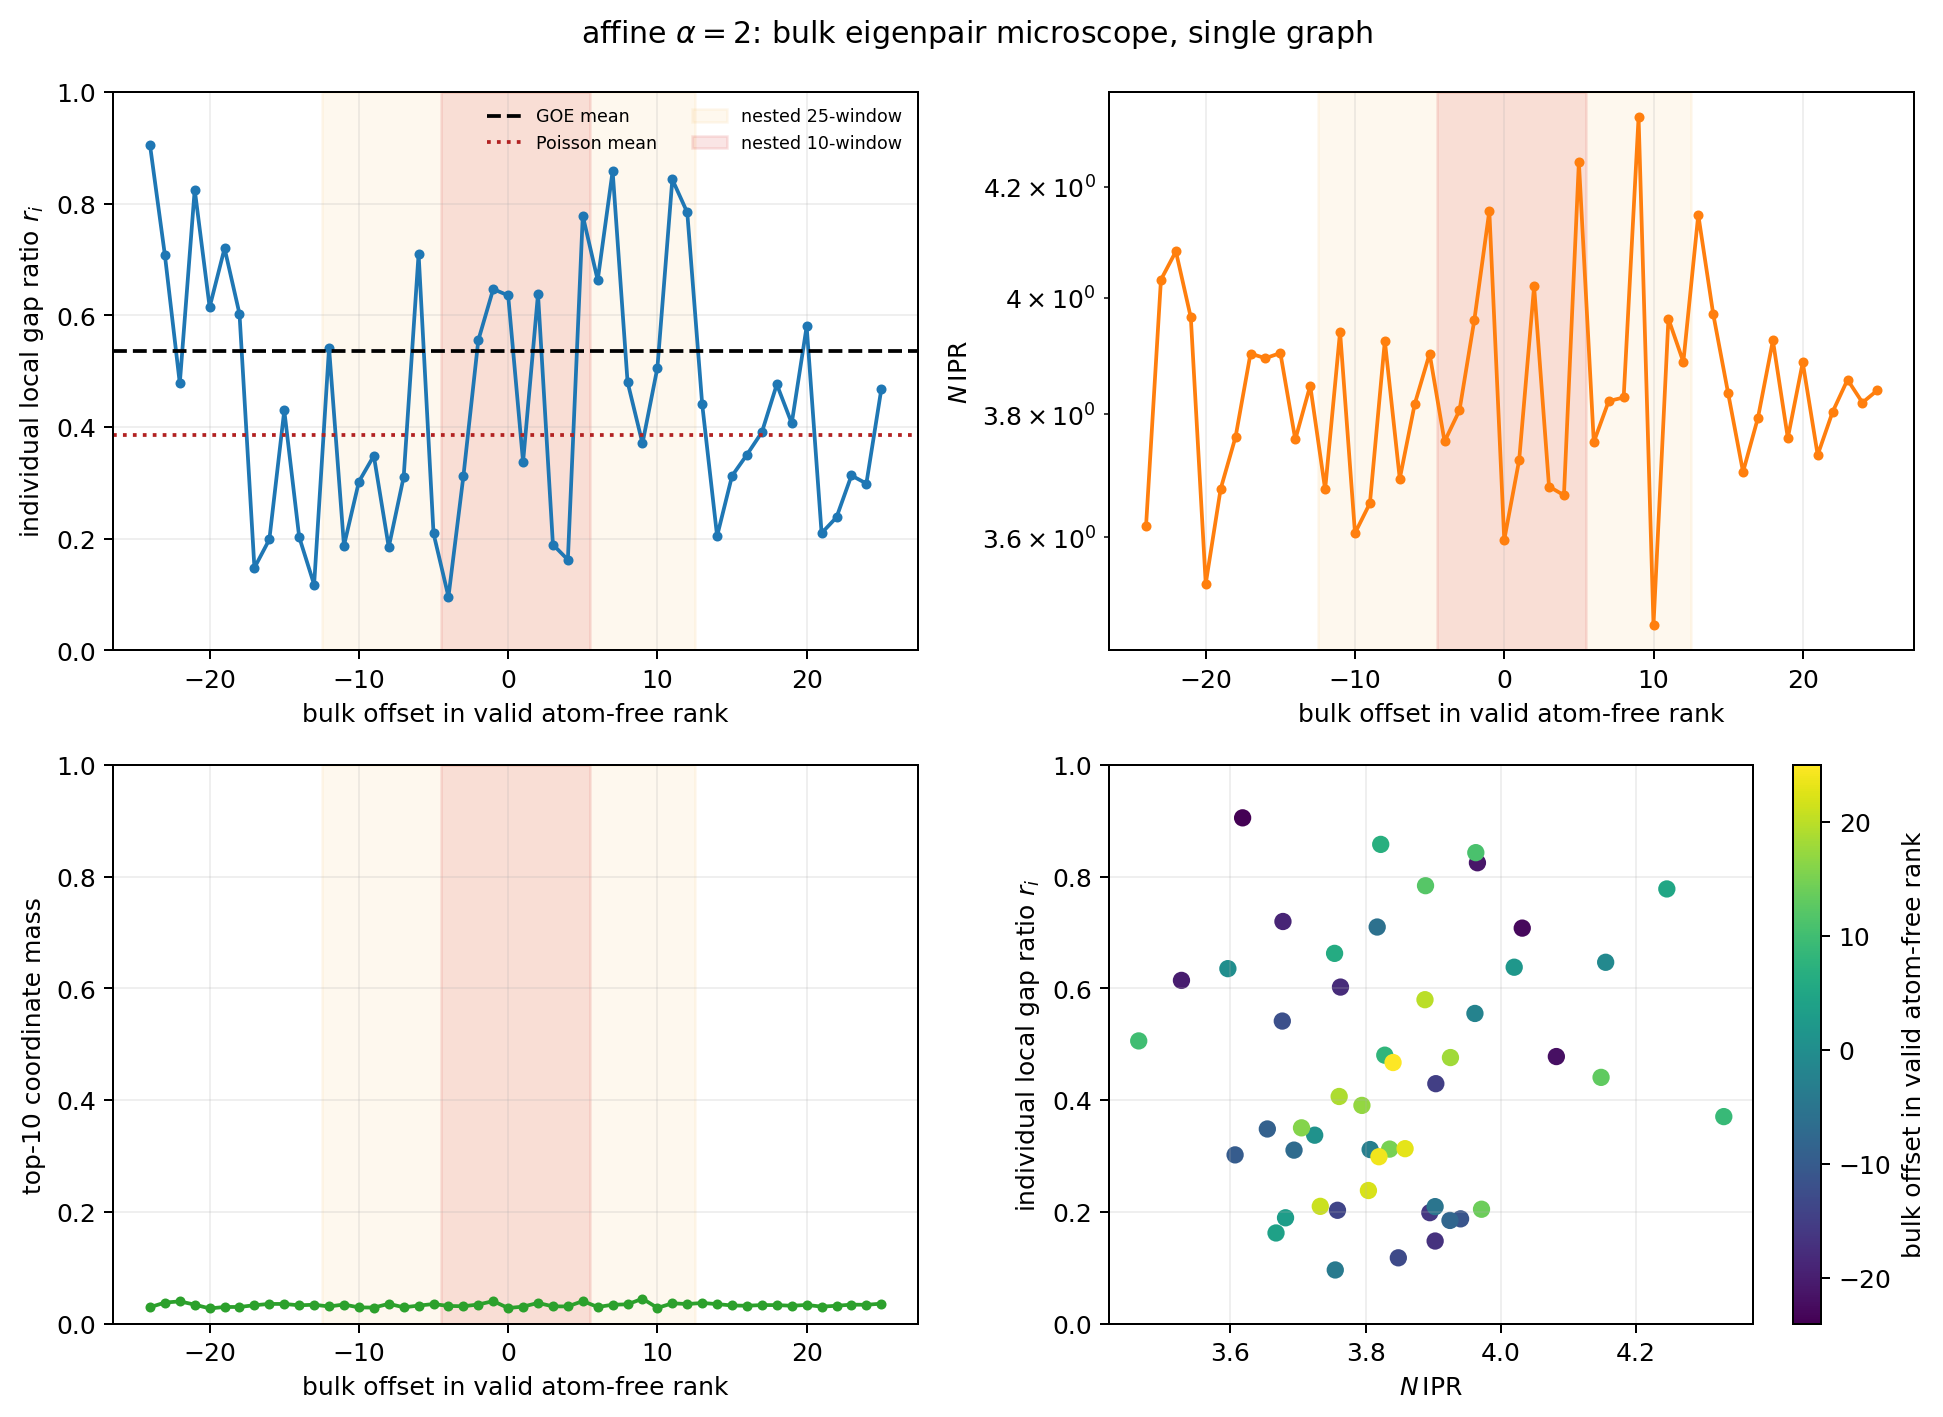
\includegraphics[width=.94\linewidth]{figures/affine_alpha_2p0/bulk/bulk_offset_diagnostics.png}
\caption{Original four-panel centered bulk-offset eigenpair microscope for affine $\alpha=2.0$.}\end{figure}
\paragraph{Direct edge-versus-bulk comparison.} Every eigenvector/support metric separates edge and bulk: edge $N\,\mathrm{IPR}$ and $M_{10}$ are much larger, its selected vertices have degrees in the hundreds rather than about ten, induced density is substantial rather than zero, and pairwise distance is roughly 1--2 rather than about 3. The strongly negative distance z-scores confirm compactness relative to uniform random supports.
\begin{figure}[H]\centering
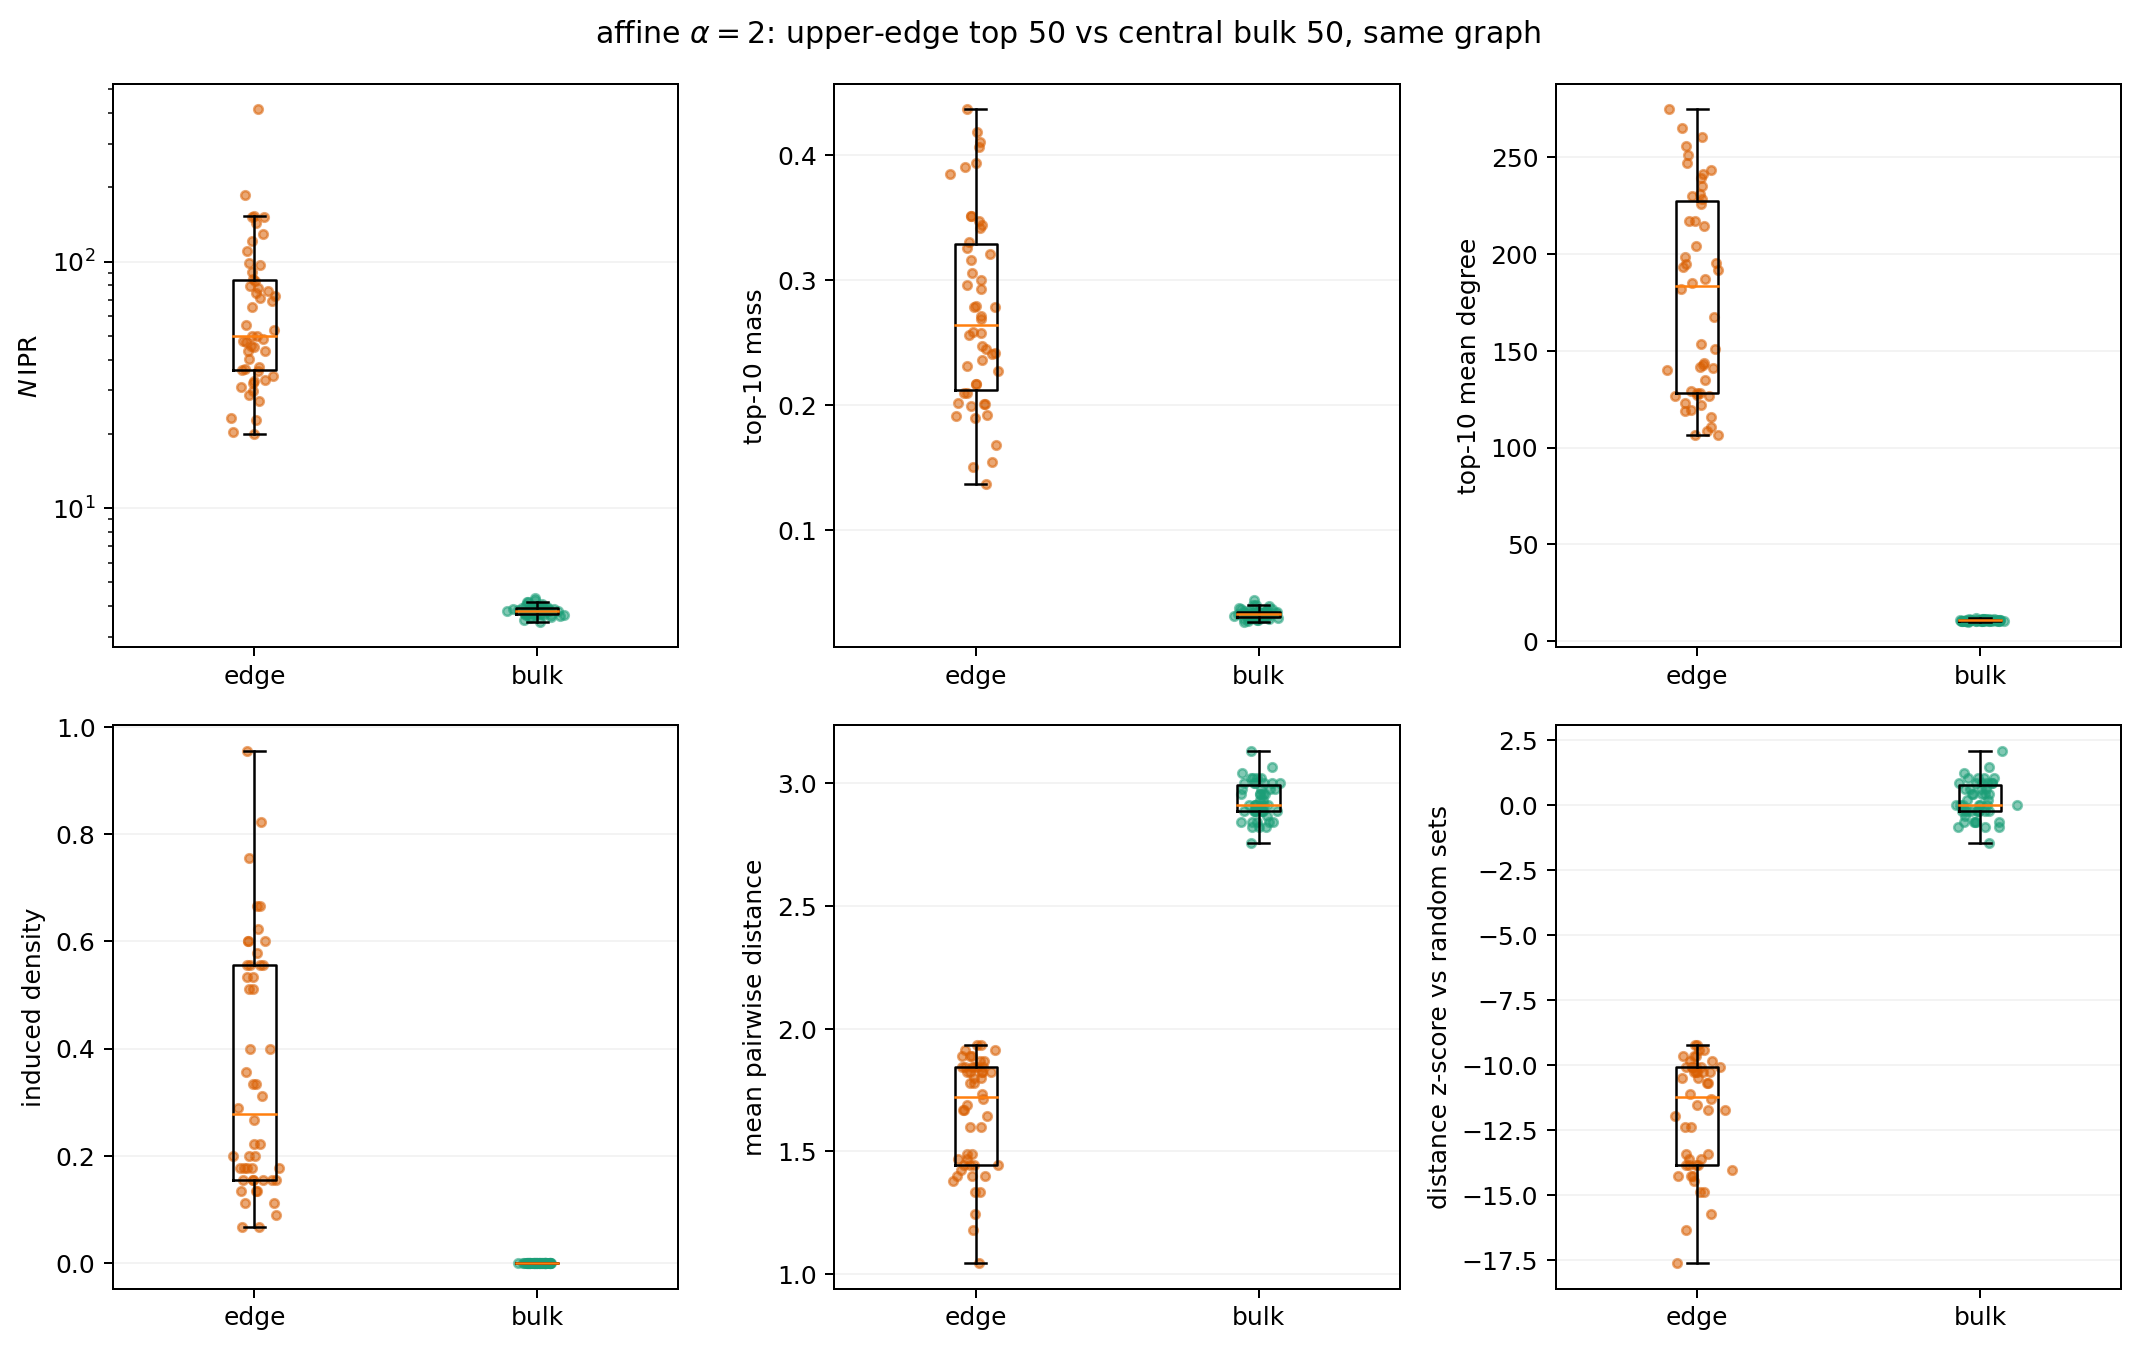
\includegraphics[width=.94\linewidth]{figures/affine_alpha_2p0/edge_vs_bulk/edge_vs_bulk_comparison.png}
\caption{Original direct edge-versus-bulk comparison for affine $\alpha=2.0$.}\end{figure}
\section{Original induced top-mass support graphs}
These are the original test drawings: edge ranks 1--10 include the Perron state at rank 1, and the bulk panels are the centered zero-eigenvalue-free bulk-10 window. They are retained exactly as recorded; no replacement or newly generated induced graph is included. Coordinate tables remain omitted. In every panel, the number printed inside a node is its original vertex ID in the full graph, while node area is proportional to that vertex's eigenvector mass $|v_j|^2$; node color, not node size, encodes its full-graph degree.
Across the three models, the edge drawings visually agree with the numerical density, component, LCC, degree, and distance summaries: the selected vertices usually form one dense hub-rich component. The bulk drawings are almost edgeless, often ten singleton components. This does not contradict full-graph distances near two or three because paths through vertices outside the displayed ten are not drawn.
\subsection{affine $\alpha=1.05$: original edge ranks 1--10}
\begin{figure}[H]\centering
\begin{minipage}[t]{.48\linewidth}\centering
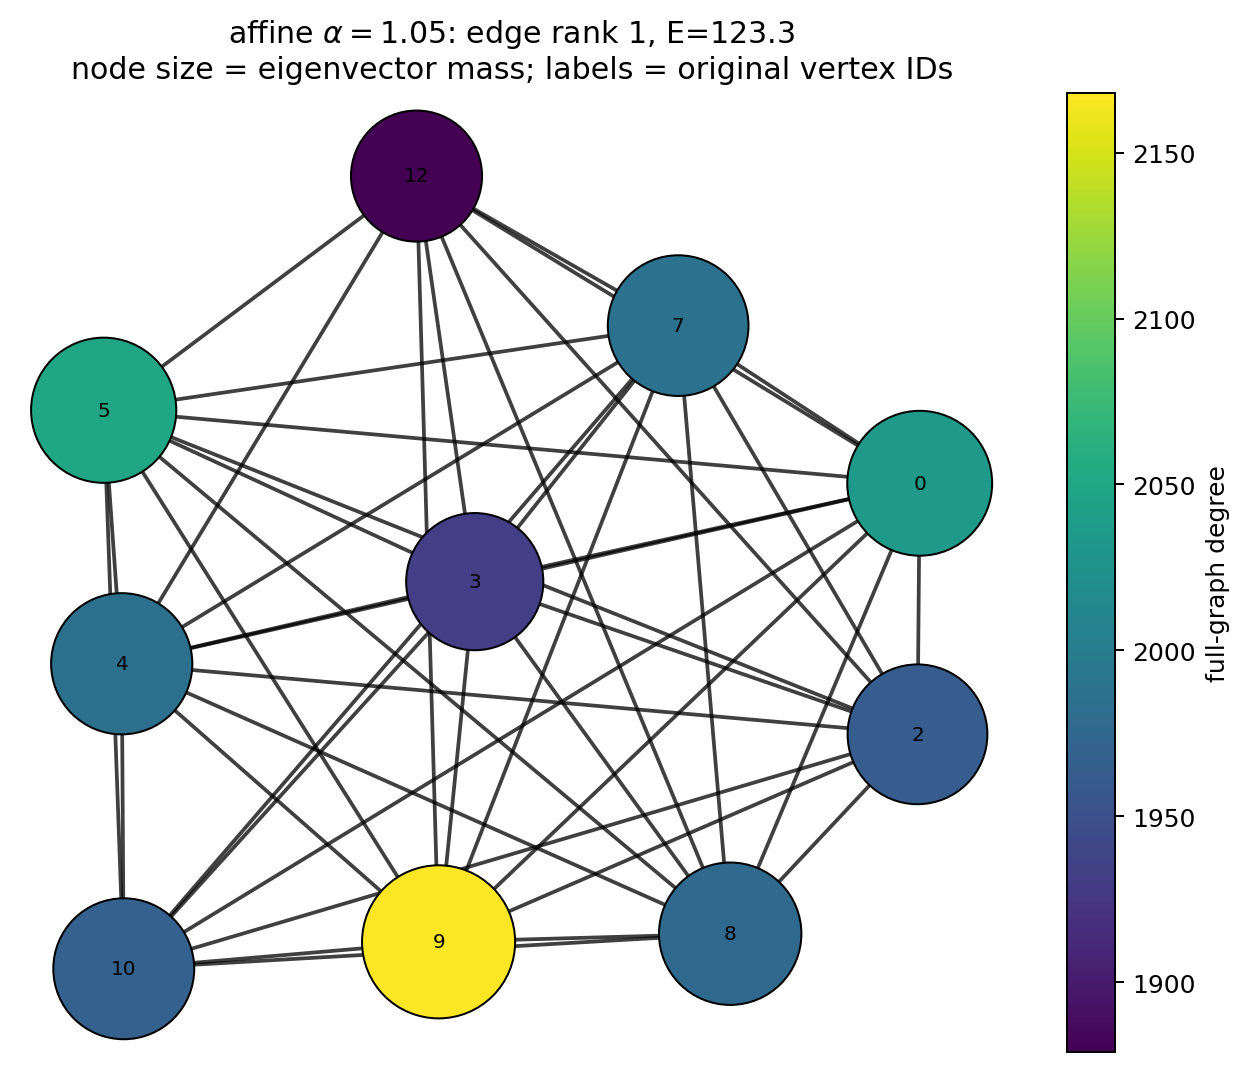
\includegraphics[width=\linewidth]{figures/affine_alpha_1p05/induced_subgraphs/edge/edge_rank_001.png}
\caption*{\footnotesize edge rank 001}\end{minipage}
\hfill
\begin{minipage}[t]{.48\linewidth}\centering
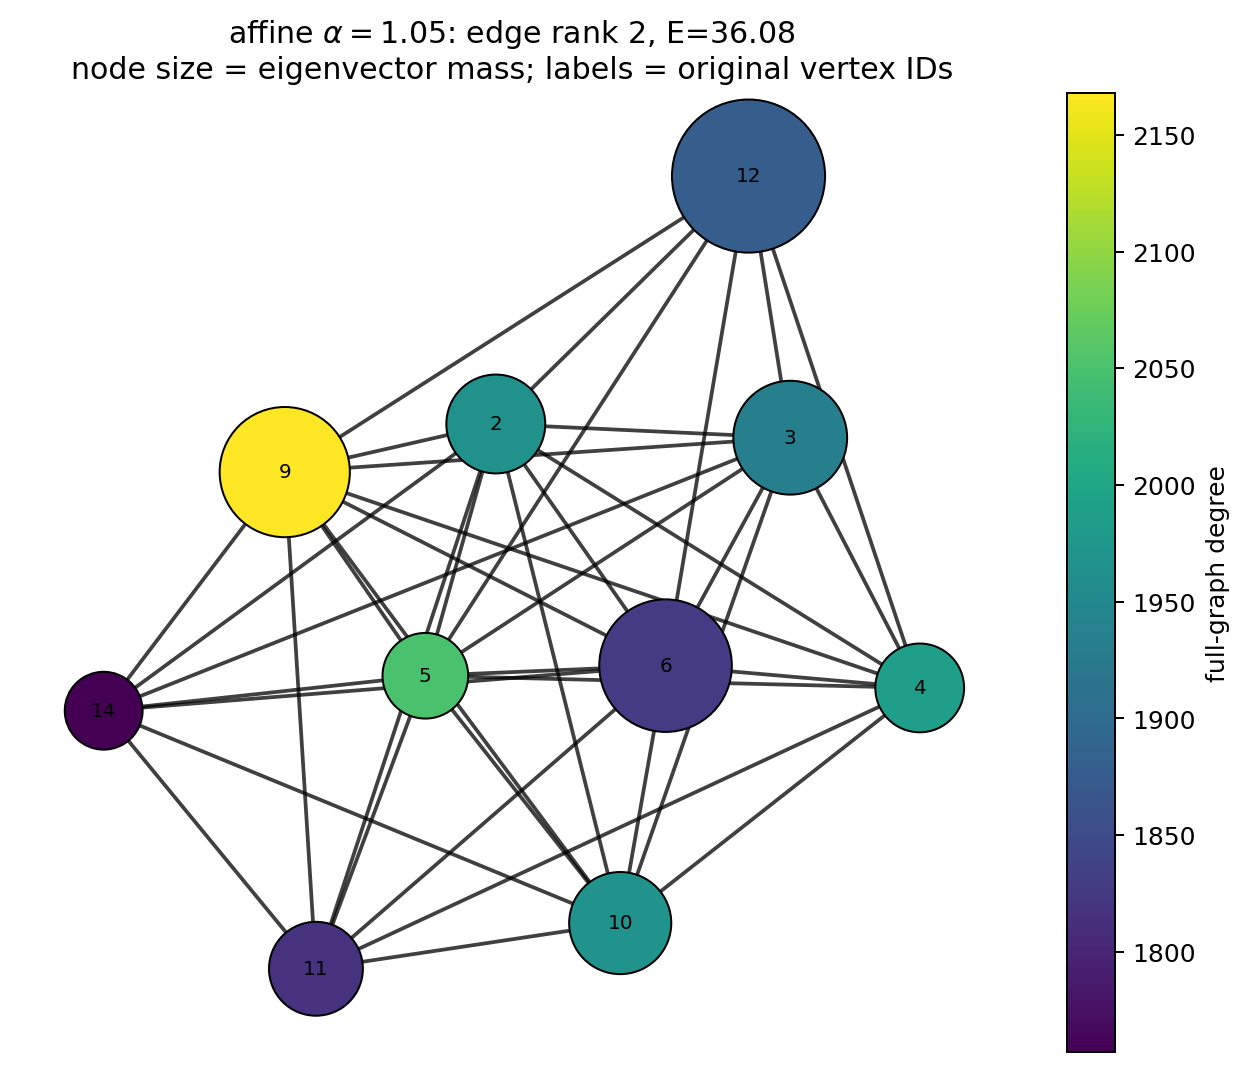
\includegraphics[width=\linewidth]{figures/affine_alpha_1p05/induced_subgraphs/edge/edge_rank_002.png}
\caption*{\footnotesize edge rank 002}\end{minipage}
\par\medskip
\begin{minipage}[t]{.48\linewidth}\centering
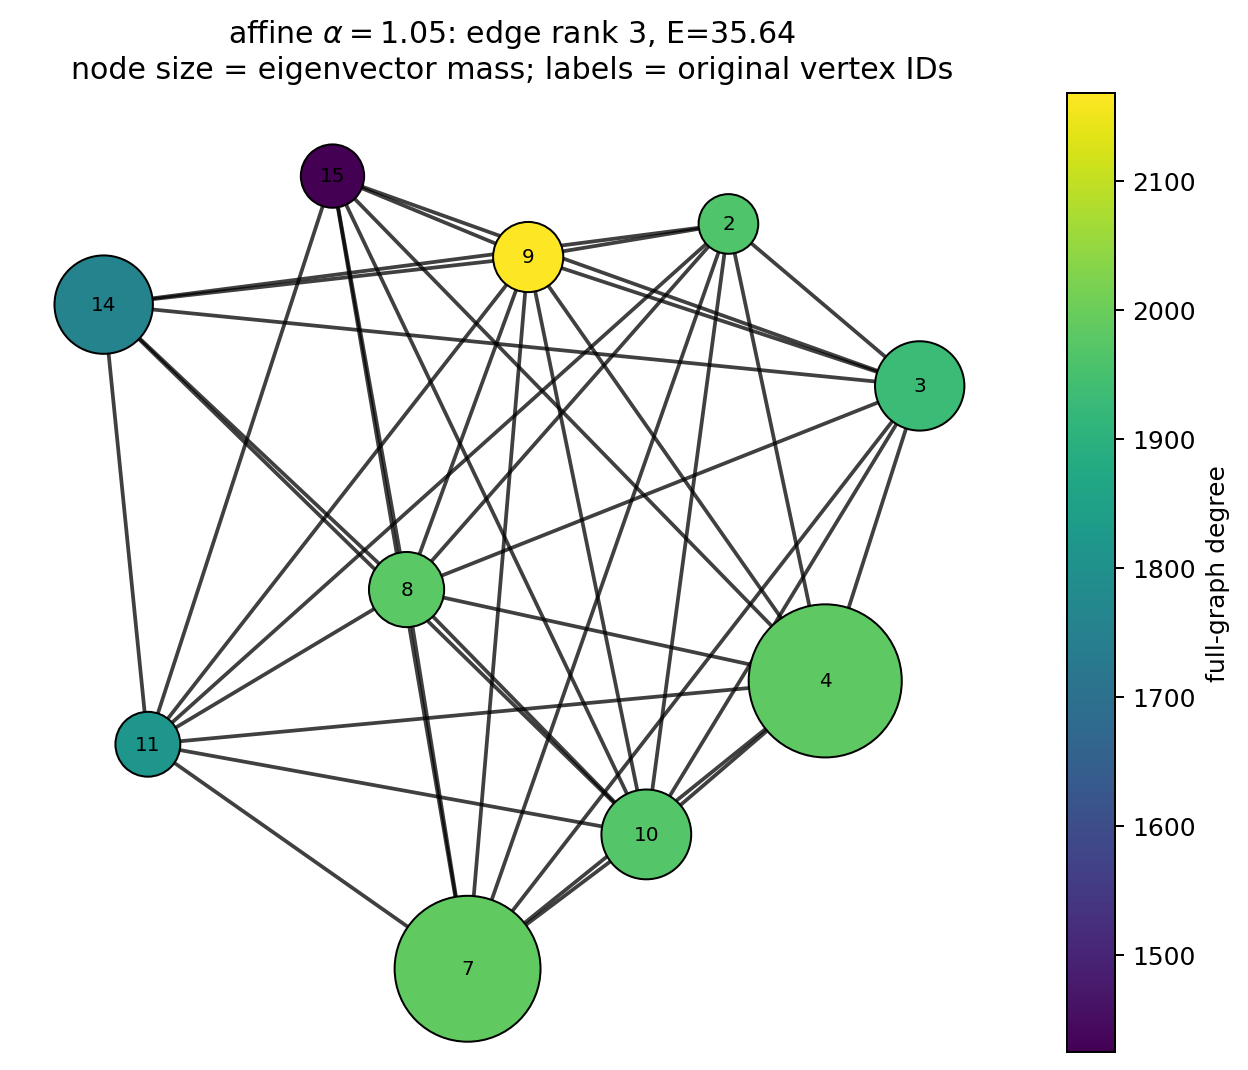
\includegraphics[width=\linewidth]{figures/affine_alpha_1p05/induced_subgraphs/edge/edge_rank_003.png}
\caption*{\footnotesize edge rank 003}\end{minipage}
\hfill
\begin{minipage}[t]{.48\linewidth}\centering
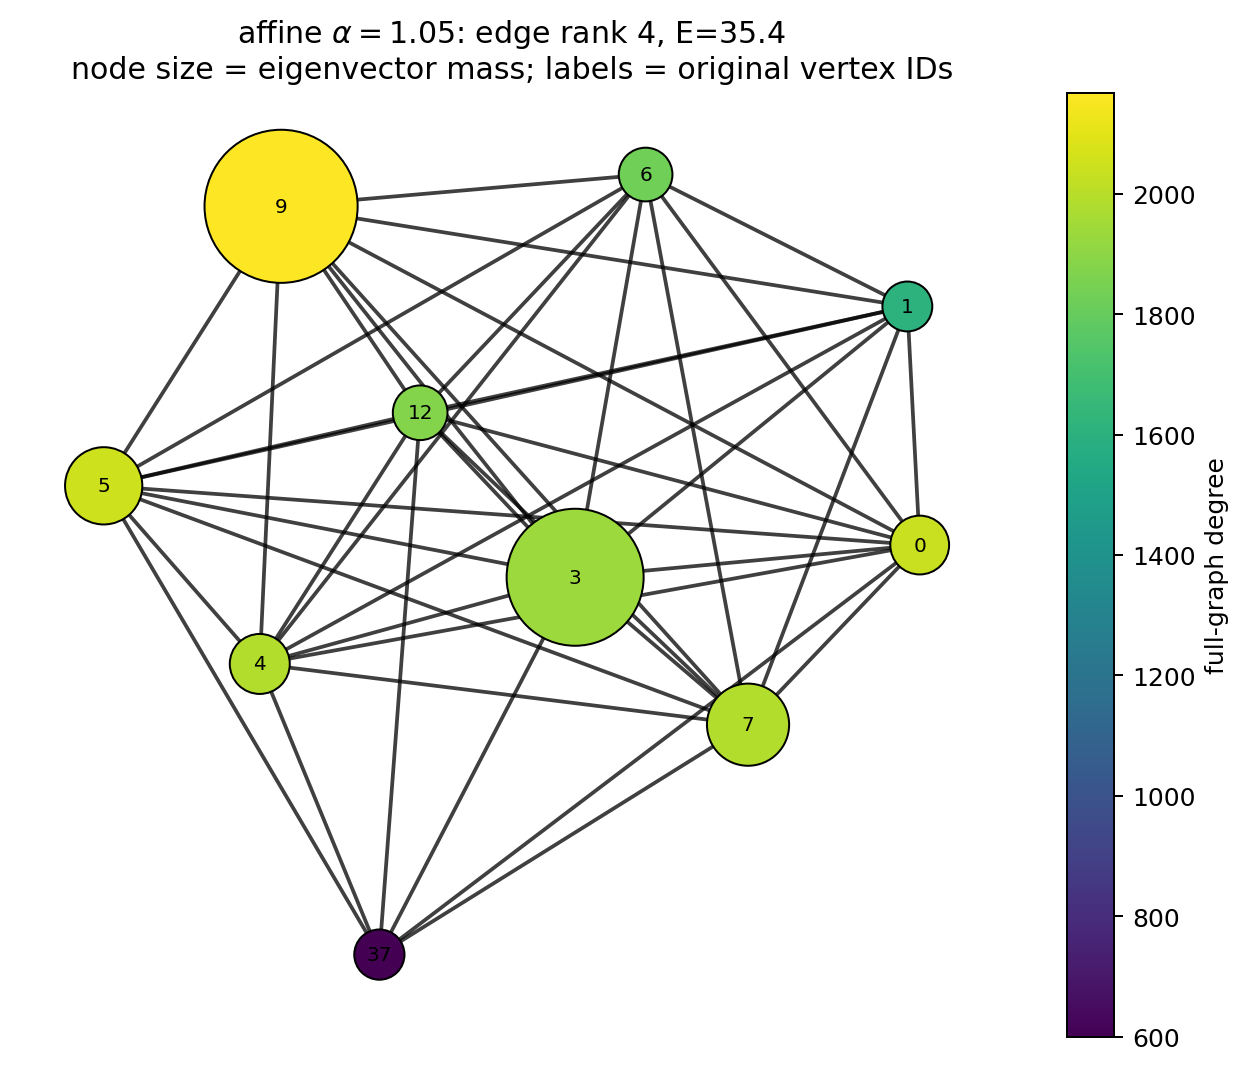
\includegraphics[width=\linewidth]{figures/affine_alpha_1p05/induced_subgraphs/edge/edge_rank_004.png}
\caption*{\footnotesize edge rank 004}\end{minipage}
\caption{Original edge induced supports, ranks 1--4.}\end{figure}
\begin{figure}[H]\centering
\begin{minipage}[t]{.48\linewidth}\centering
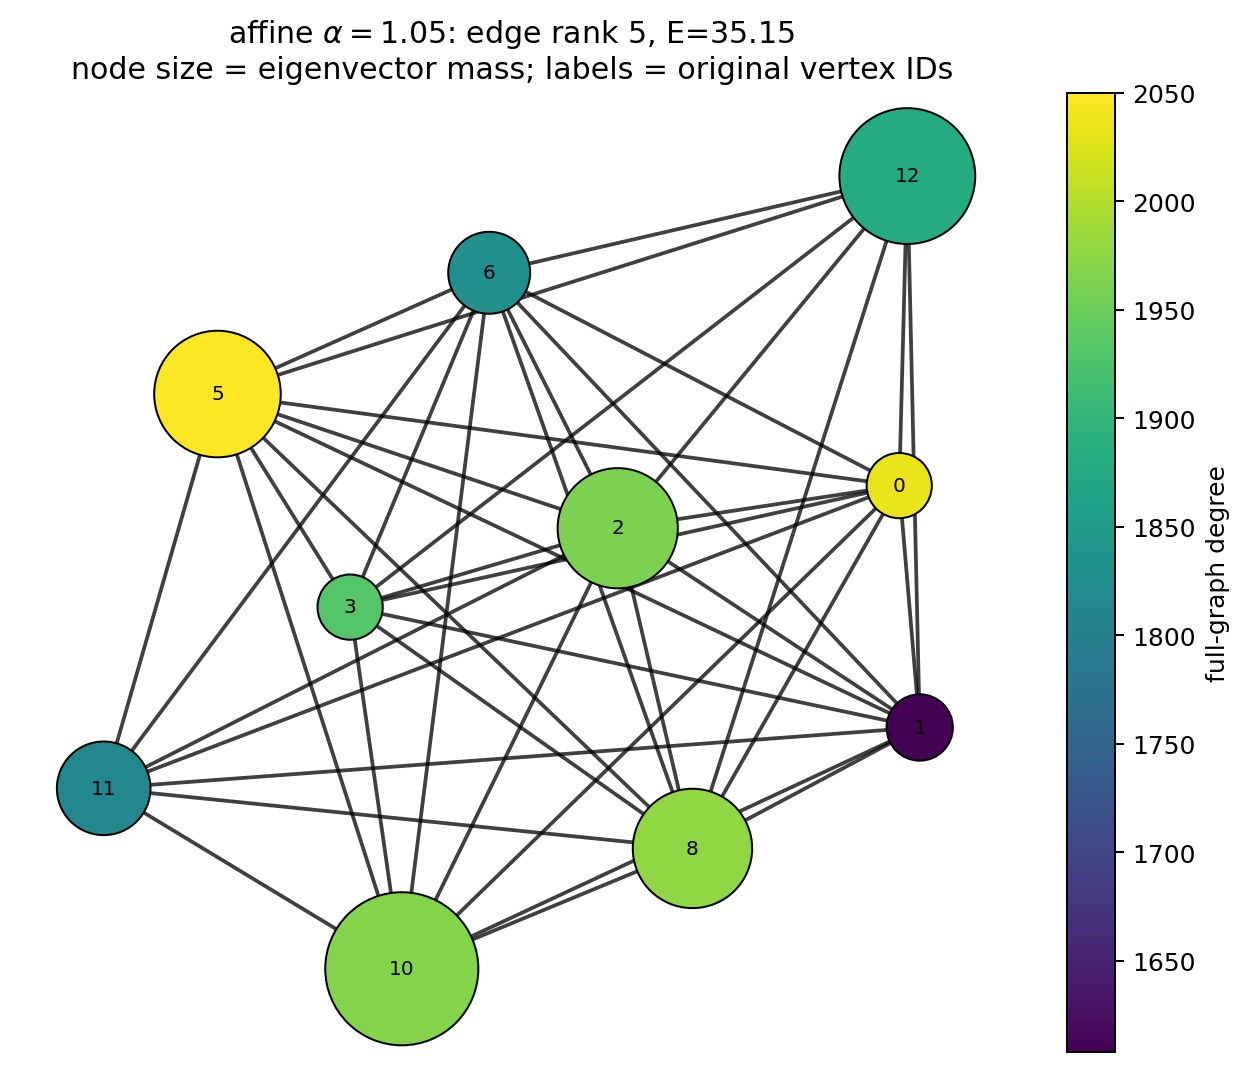
\includegraphics[width=\linewidth]{figures/affine_alpha_1p05/induced_subgraphs/edge/edge_rank_005.png}
\caption*{\footnotesize edge rank 005}\end{minipage}
\hfill
\begin{minipage}[t]{.48\linewidth}\centering
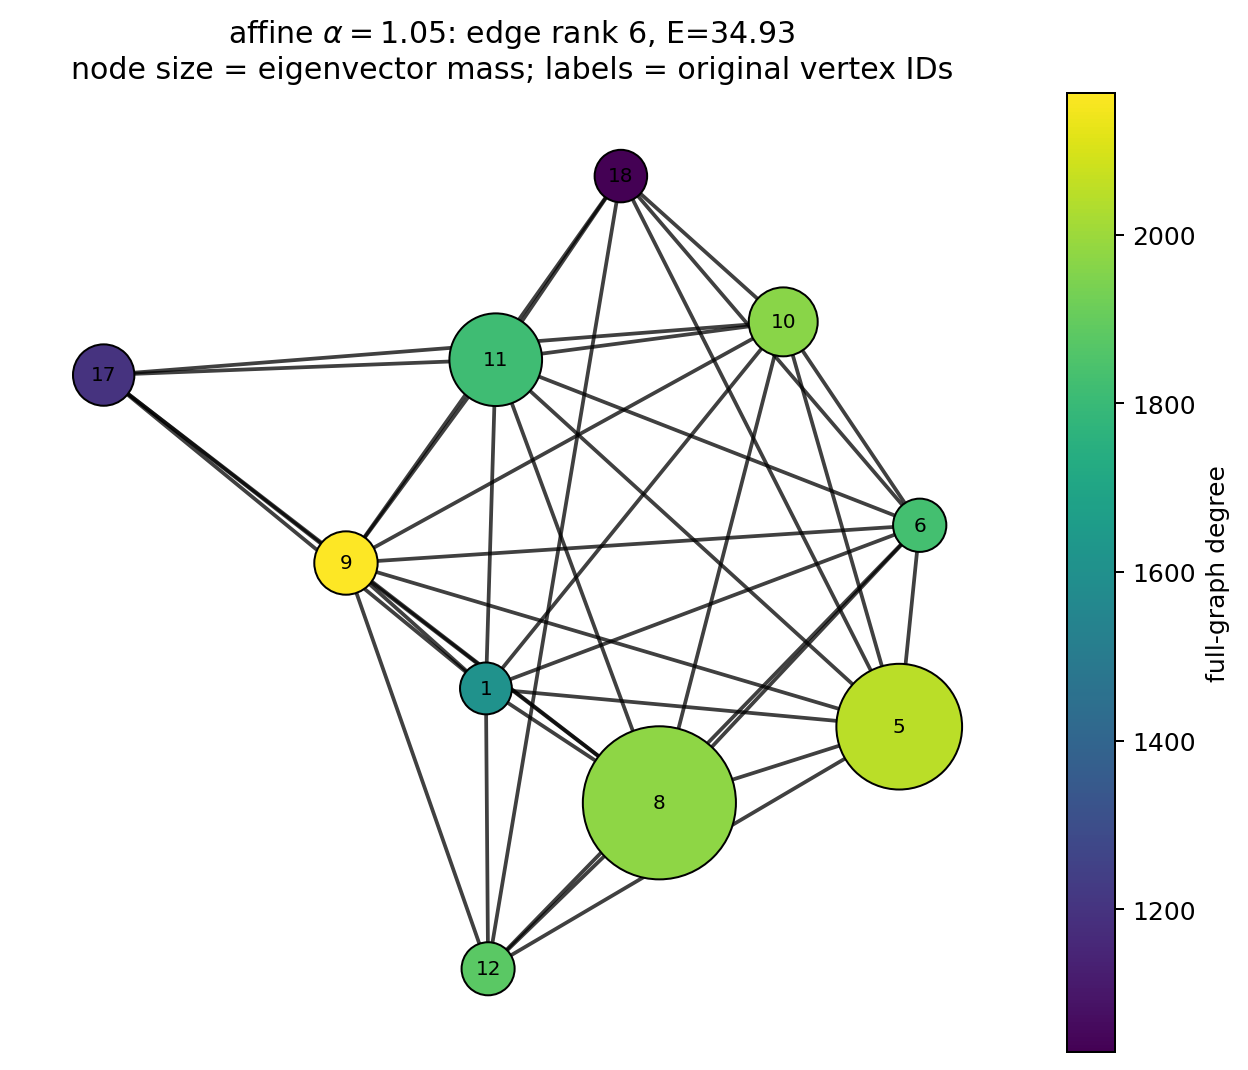
\includegraphics[width=\linewidth]{figures/affine_alpha_1p05/induced_subgraphs/edge/edge_rank_006.png}
\caption*{\footnotesize edge rank 006}\end{minipage}
\par\medskip
\begin{minipage}[t]{.48\linewidth}\centering
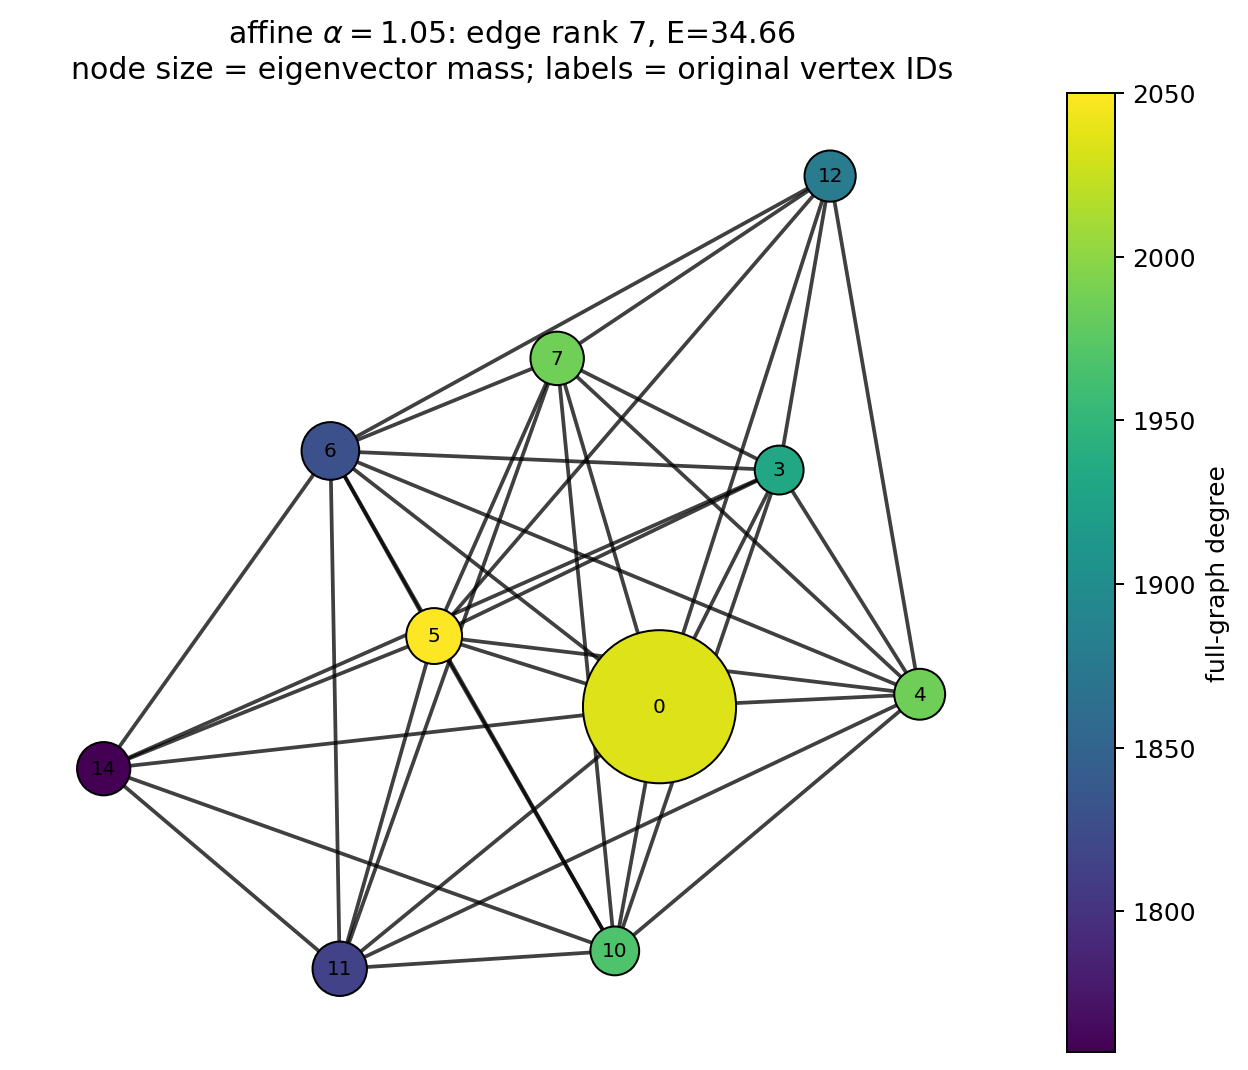
\includegraphics[width=\linewidth]{figures/affine_alpha_1p05/induced_subgraphs/edge/edge_rank_007.png}
\caption*{\footnotesize edge rank 007}\end{minipage}
\hfill
\begin{minipage}[t]{.48\linewidth}\centering
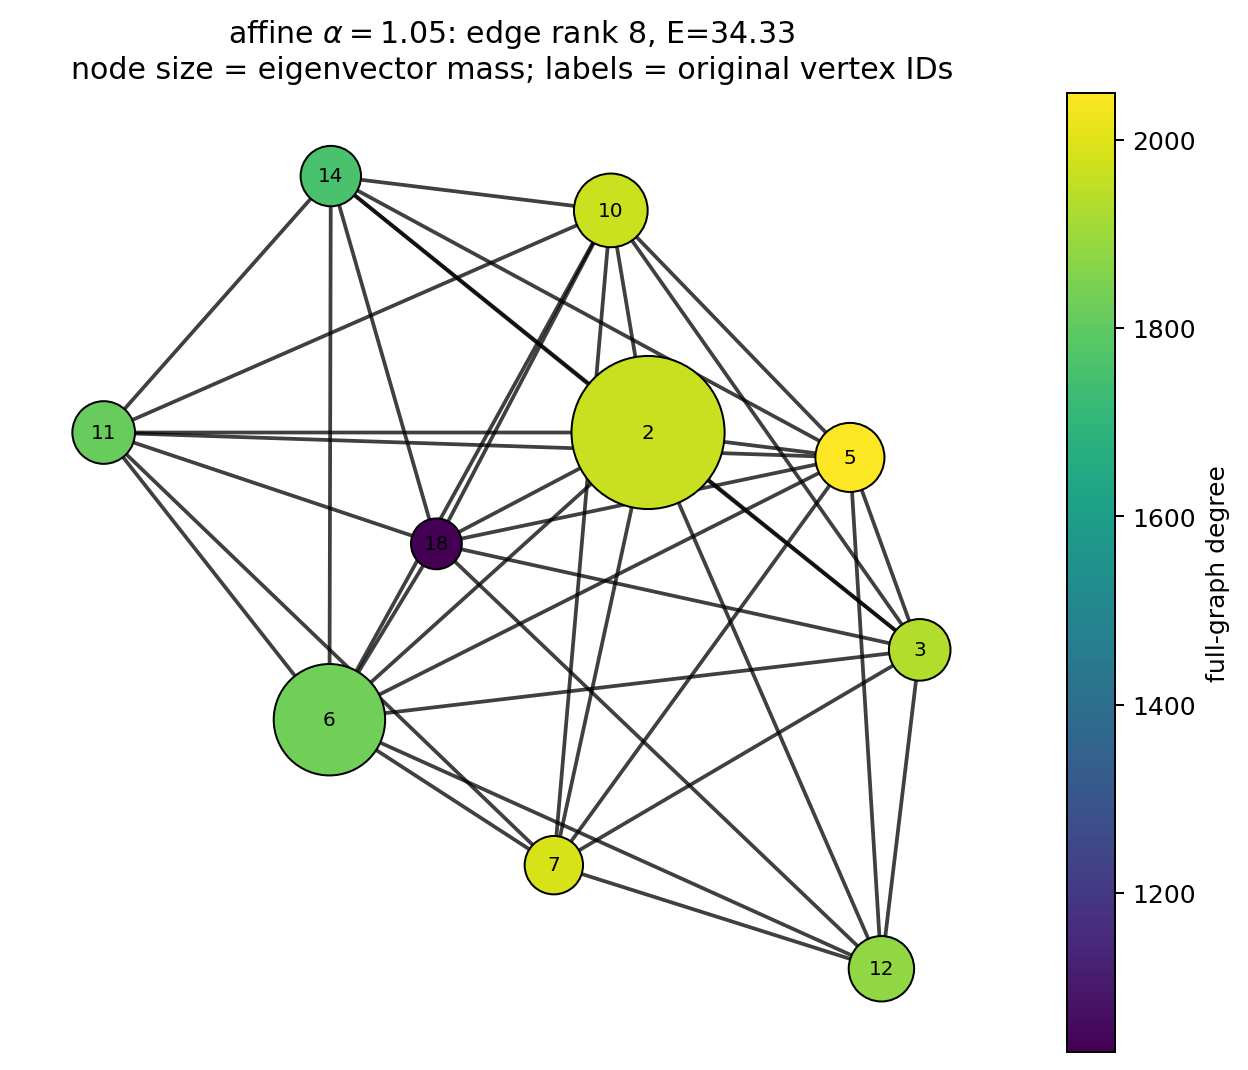
\includegraphics[width=\linewidth]{figures/affine_alpha_1p05/induced_subgraphs/edge/edge_rank_008.png}
\caption*{\footnotesize edge rank 008}\end{minipage}
\caption{Original edge induced supports, ranks 5--8.}\end{figure}
\begin{figure}[H]\centering
\begin{minipage}[t]{.48\linewidth}\centering
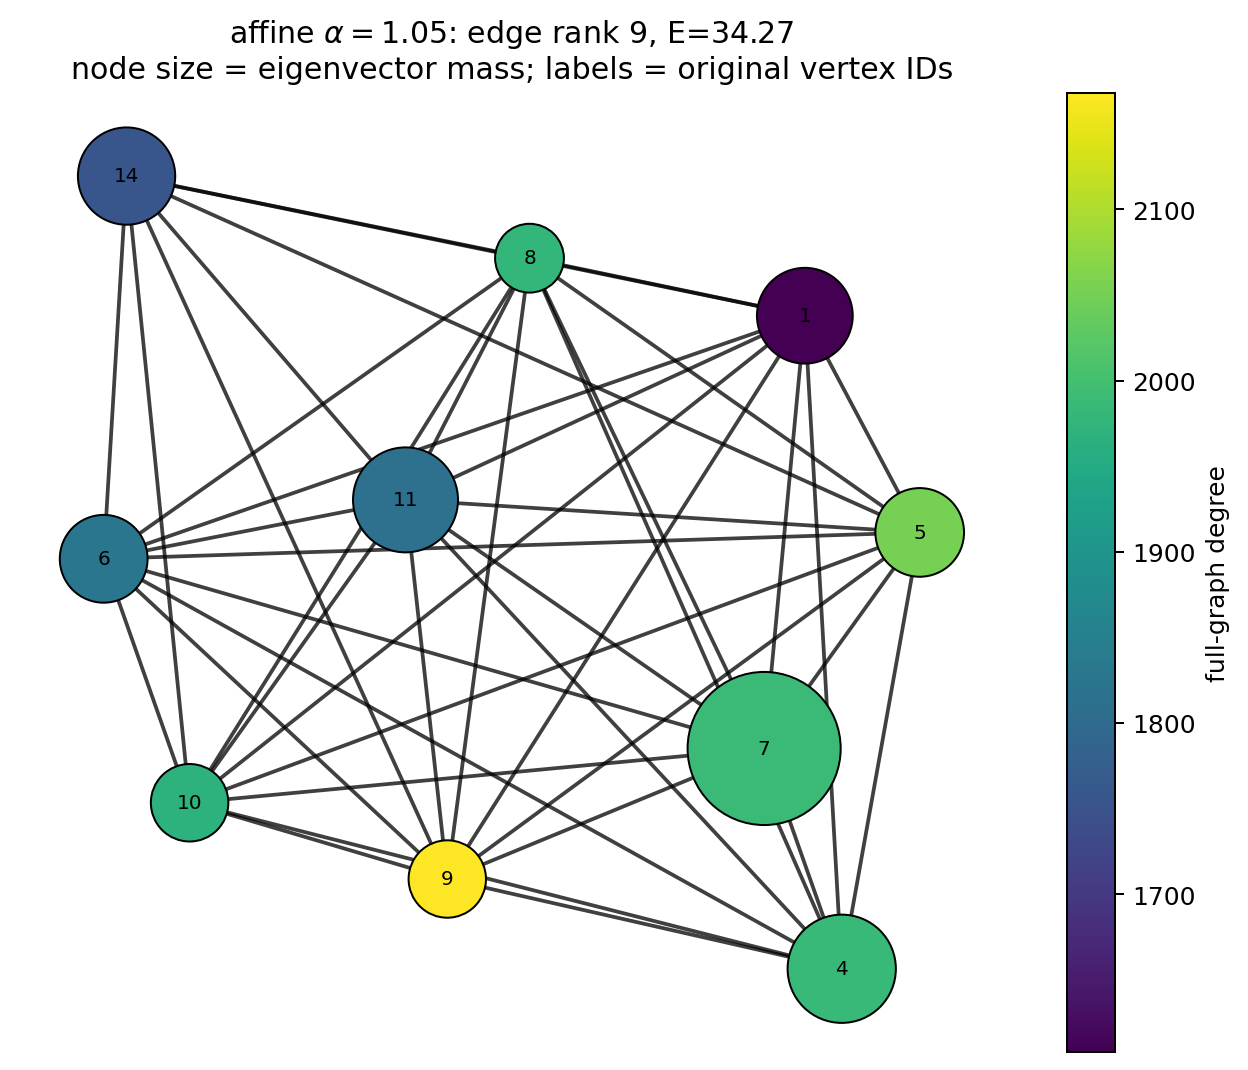
\includegraphics[width=\linewidth]{figures/affine_alpha_1p05/induced_subgraphs/edge/edge_rank_009.png}
\caption*{\footnotesize edge rank 009}\end{minipage}
\hfill
\begin{minipage}[t]{.48\linewidth}\centering
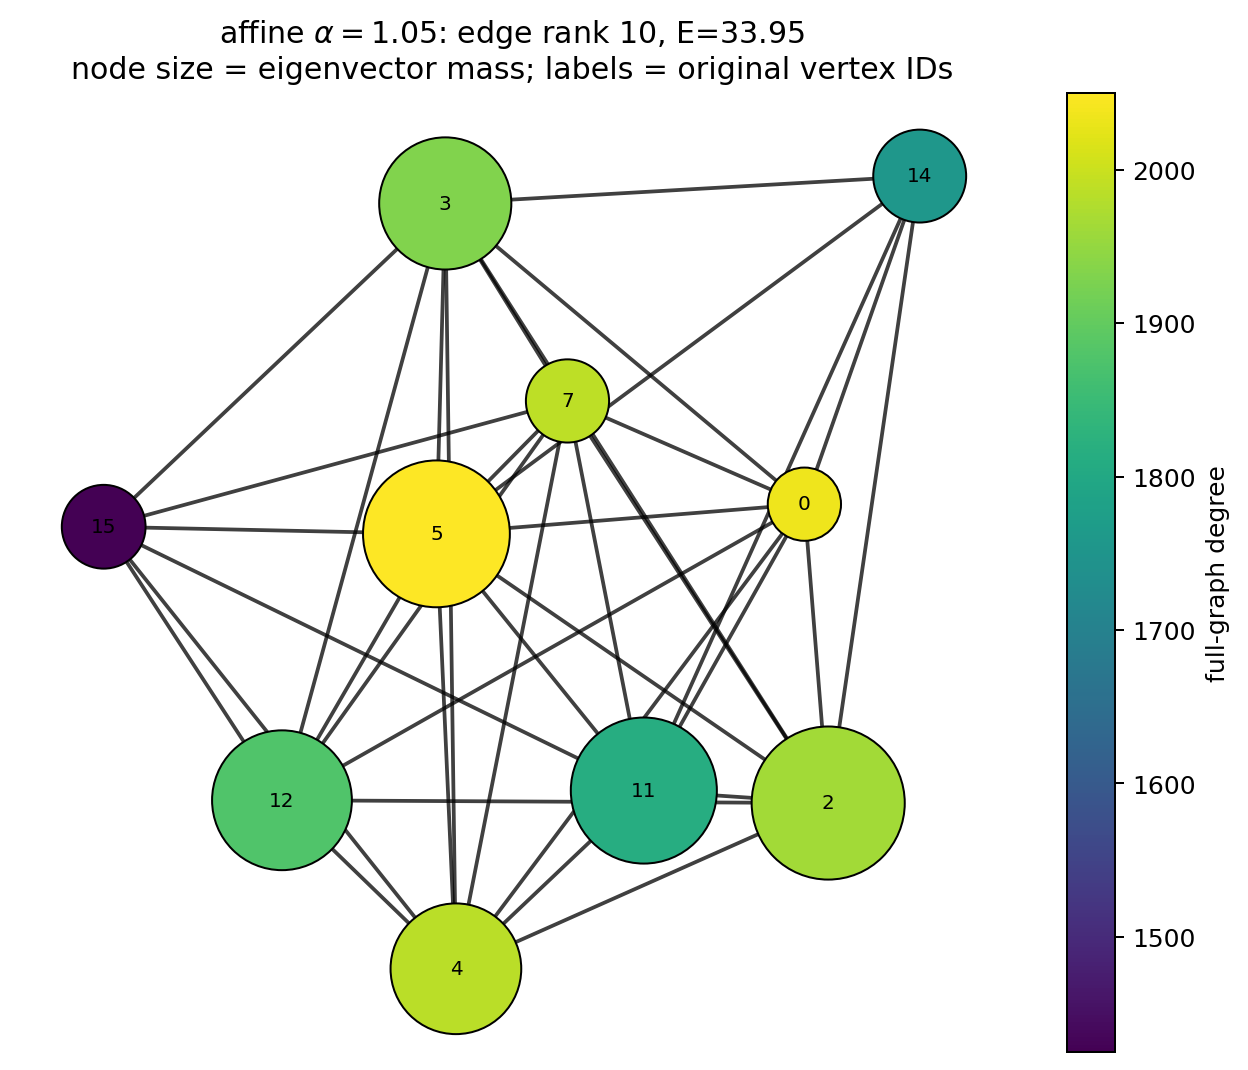
\includegraphics[width=\linewidth]{figures/affine_alpha_1p05/induced_subgraphs/edge/edge_rank_010.png}
\caption*{\footnotesize edge rank 010}\end{minipage}
\caption{Original edge induced supports, ranks 9--10.}\end{figure}
\subsection{affine $\alpha=1.05$: original centered bulk window}
\begin{figure}[H]\centering
\begin{minipage}[t]{.48\linewidth}\centering
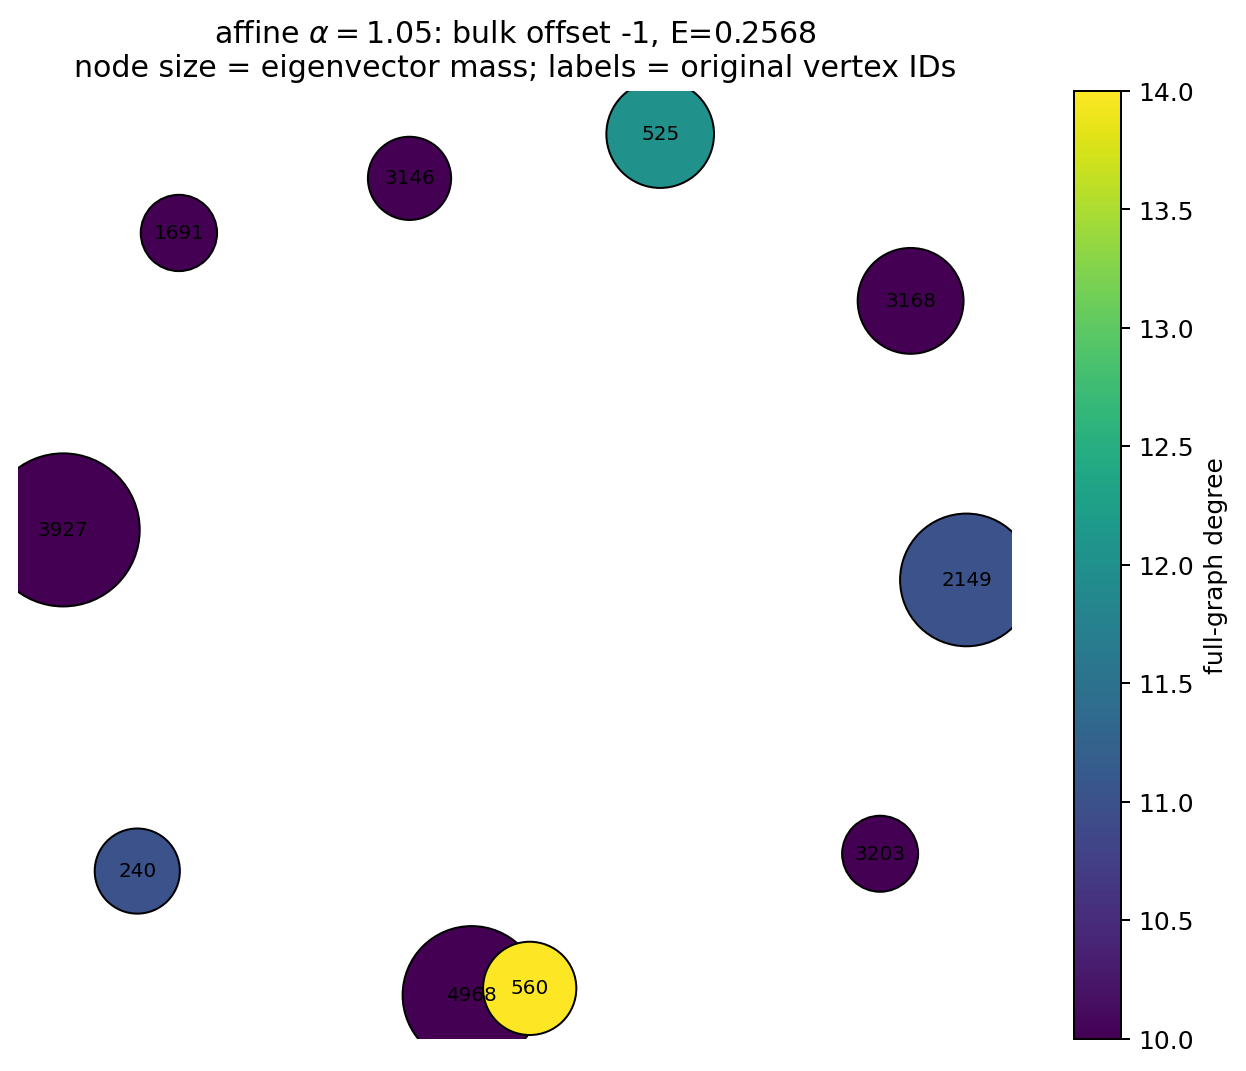
\includegraphics[width=\linewidth]{figures/affine_alpha_1p05/induced_subgraphs/bulk/bulk_offset_m001.png}
\caption*{\footnotesize bulk offset m001}\end{minipage}
\hfill
\begin{minipage}[t]{.48\linewidth}\centering
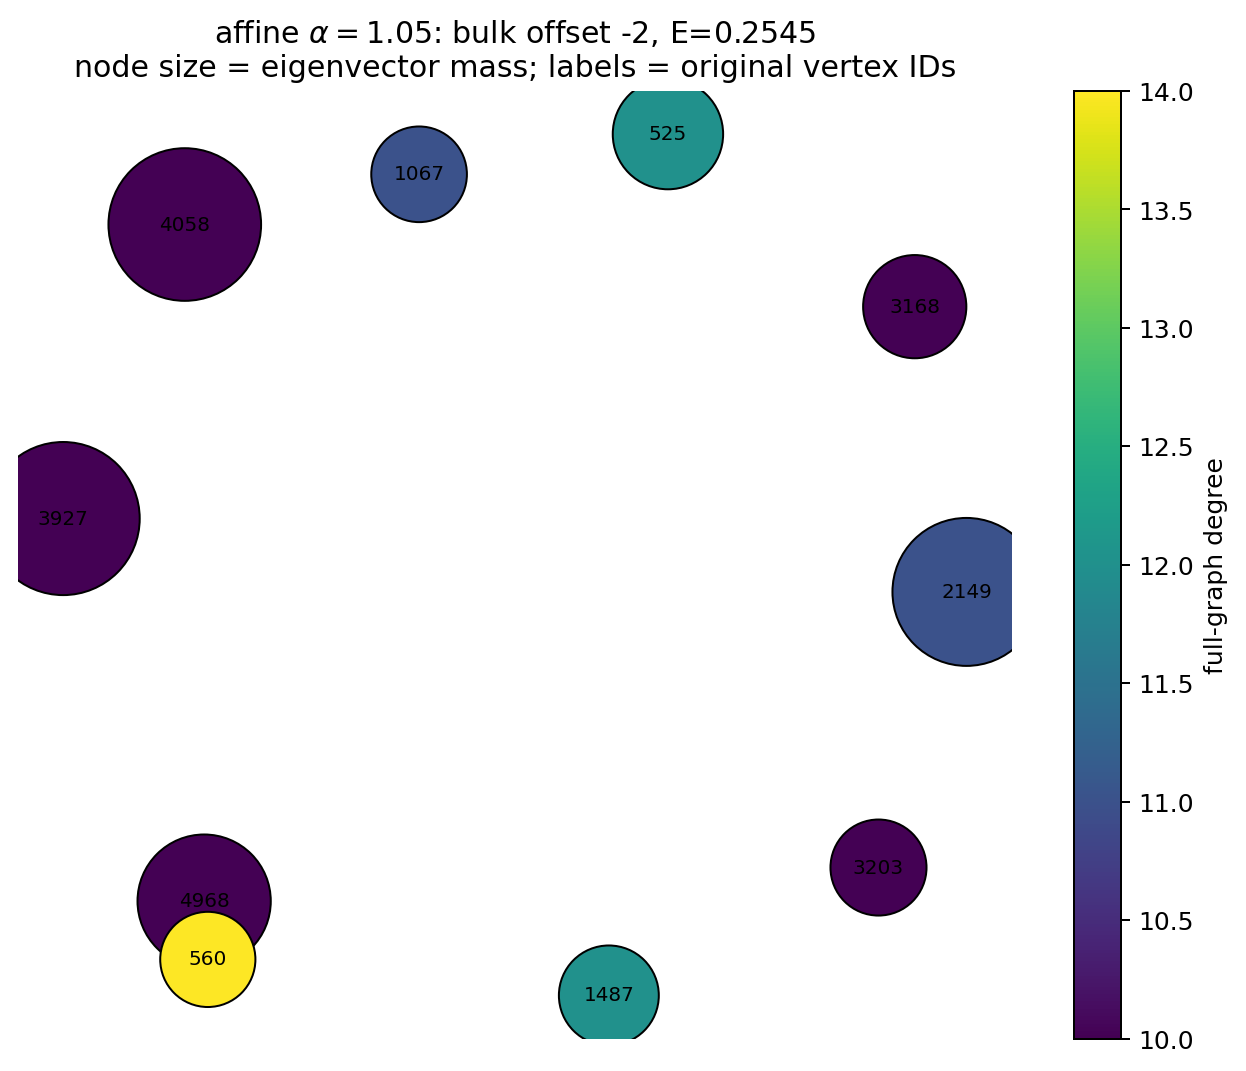
\includegraphics[width=\linewidth]{figures/affine_alpha_1p05/induced_subgraphs/bulk/bulk_offset_m002.png}
\caption*{\footnotesize bulk offset m002}\end{minipage}
\par\medskip
\begin{minipage}[t]{.48\linewidth}\centering
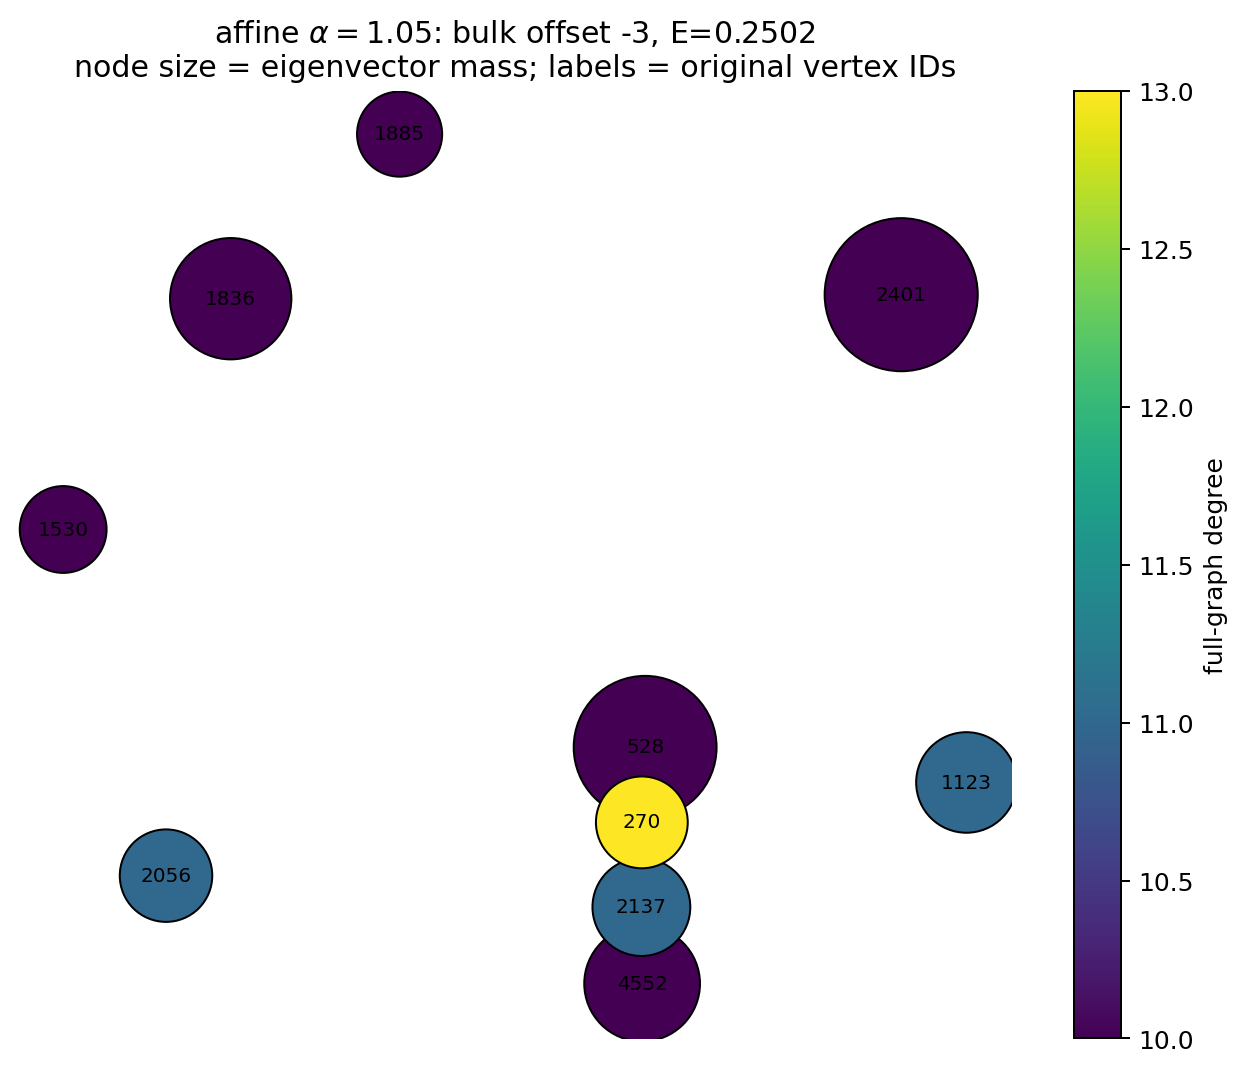
\includegraphics[width=\linewidth]{figures/affine_alpha_1p05/induced_subgraphs/bulk/bulk_offset_m003.png}
\caption*{\footnotesize bulk offset m003}\end{minipage}
\hfill
\begin{minipage}[t]{.48\linewidth}\centering
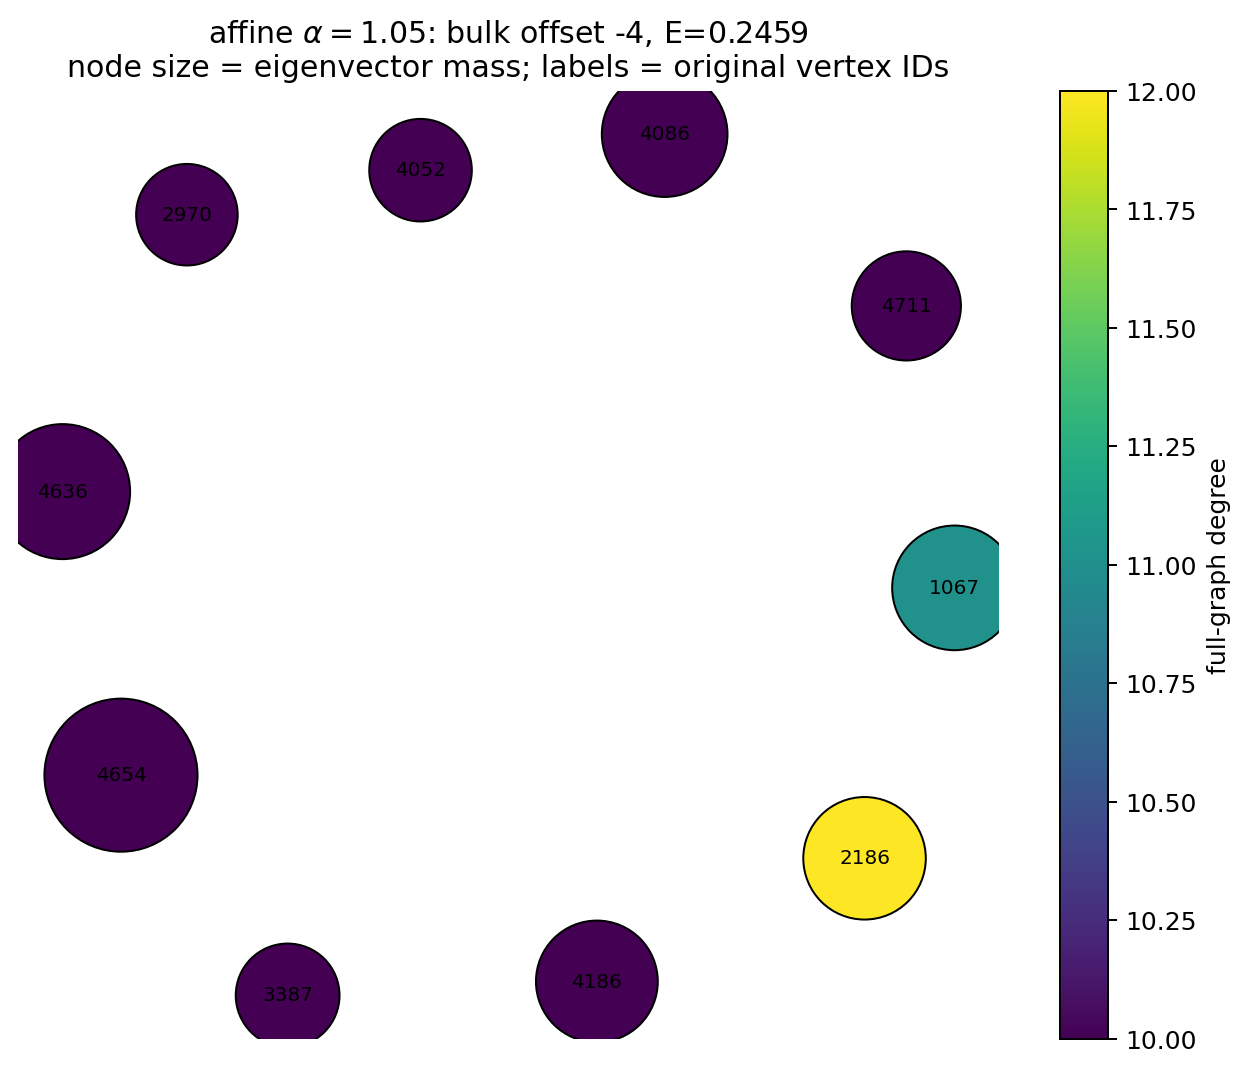
\includegraphics[width=\linewidth]{figures/affine_alpha_1p05/induced_subgraphs/bulk/bulk_offset_m004.png}
\caption*{\footnotesize bulk offset m004}\end{minipage}
\caption{Original centered bulk induced supports.}\end{figure}
\begin{figure}[H]\centering
\begin{minipage}[t]{.48\linewidth}\centering
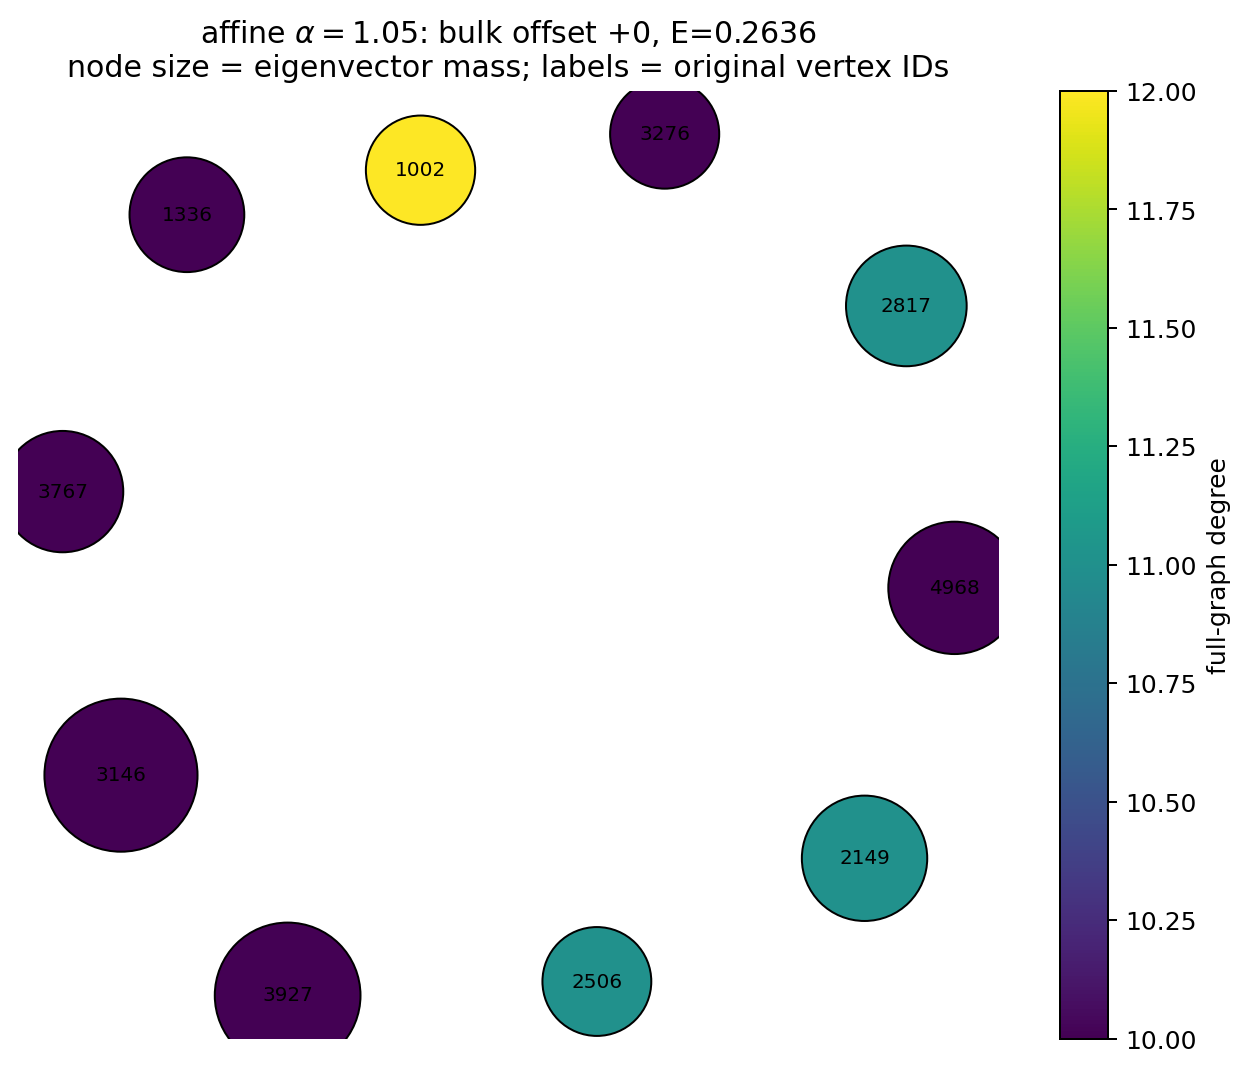
\includegraphics[width=\linewidth]{figures/affine_alpha_1p05/induced_subgraphs/bulk/bulk_offset_p000.png}
\caption*{\footnotesize bulk offset p000}\end{minipage}
\hfill
\begin{minipage}[t]{.48\linewidth}\centering
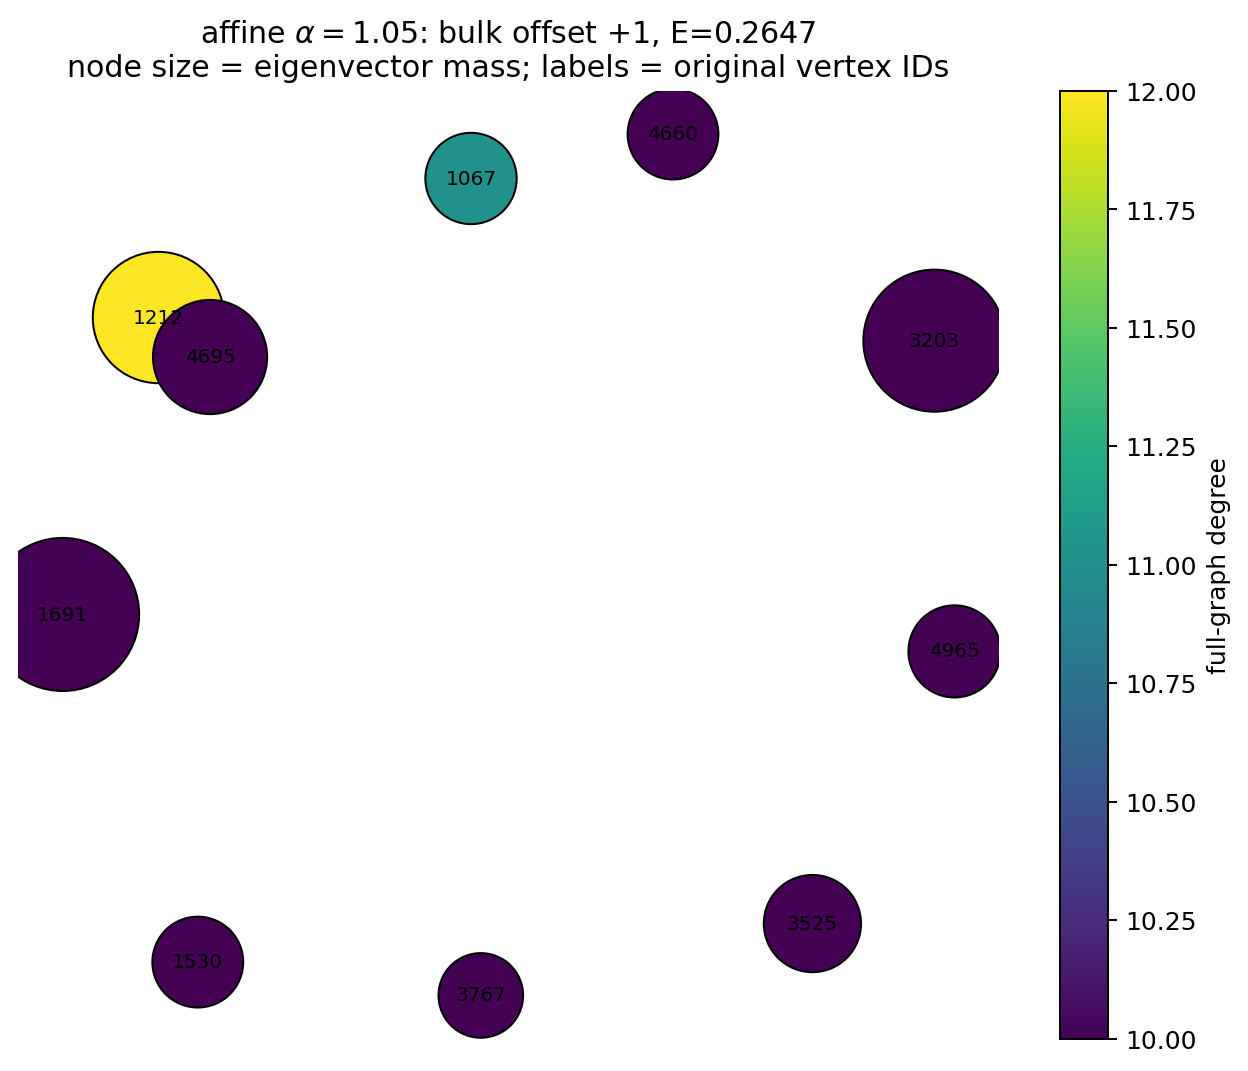
\includegraphics[width=\linewidth]{figures/affine_alpha_1p05/induced_subgraphs/bulk/bulk_offset_p001.png}
\caption*{\footnotesize bulk offset p001}\end{minipage}
\par\medskip
\begin{minipage}[t]{.48\linewidth}\centering
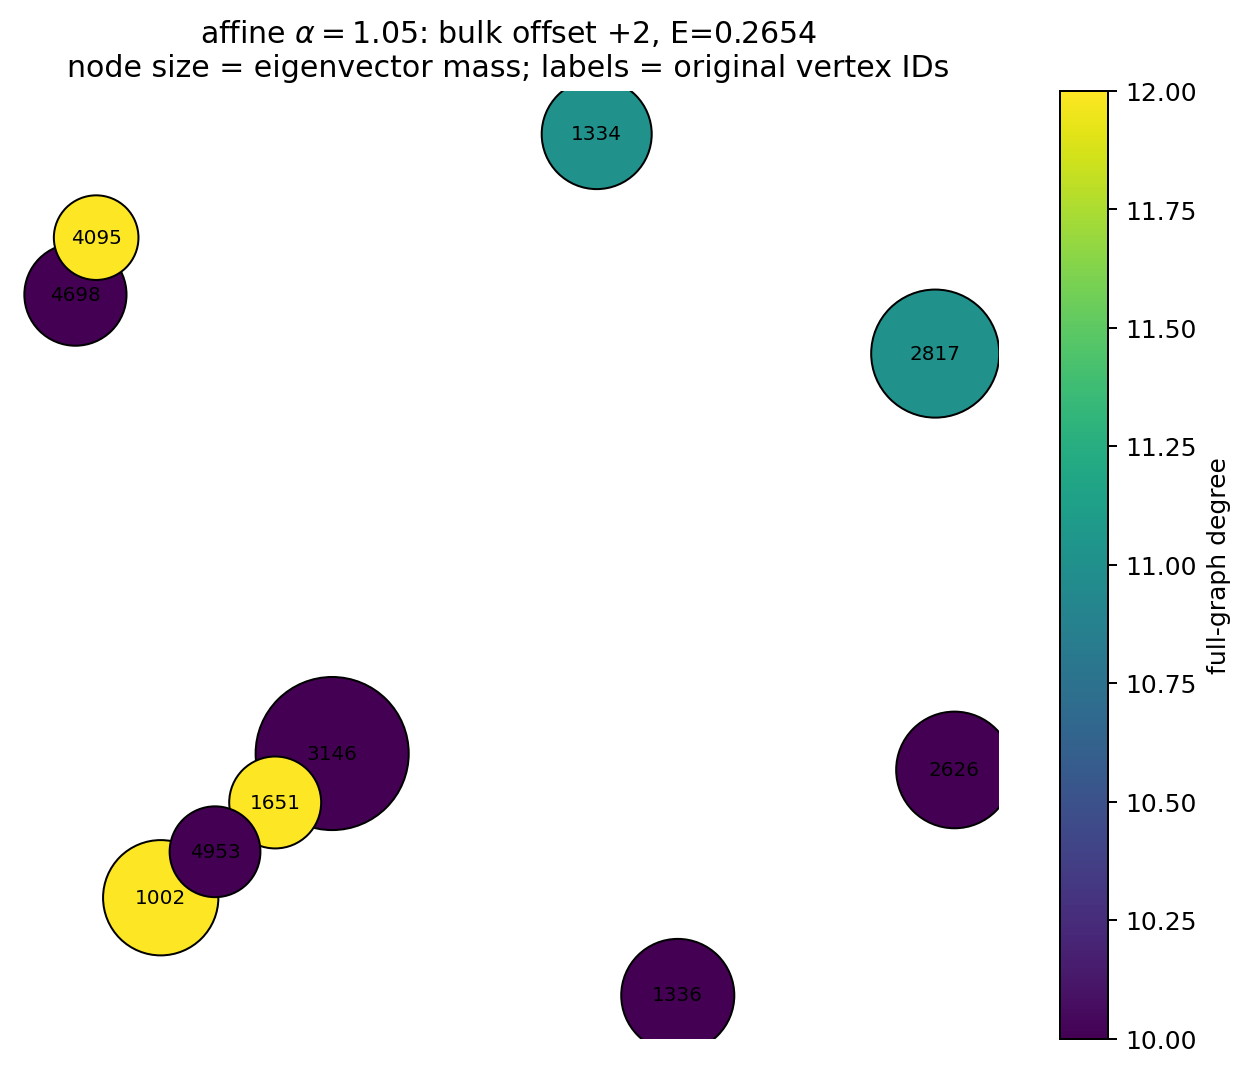
\includegraphics[width=\linewidth]{figures/affine_alpha_1p05/induced_subgraphs/bulk/bulk_offset_p002.png}
\caption*{\footnotesize bulk offset p002}\end{minipage}
\hfill
\begin{minipage}[t]{.48\linewidth}\centering
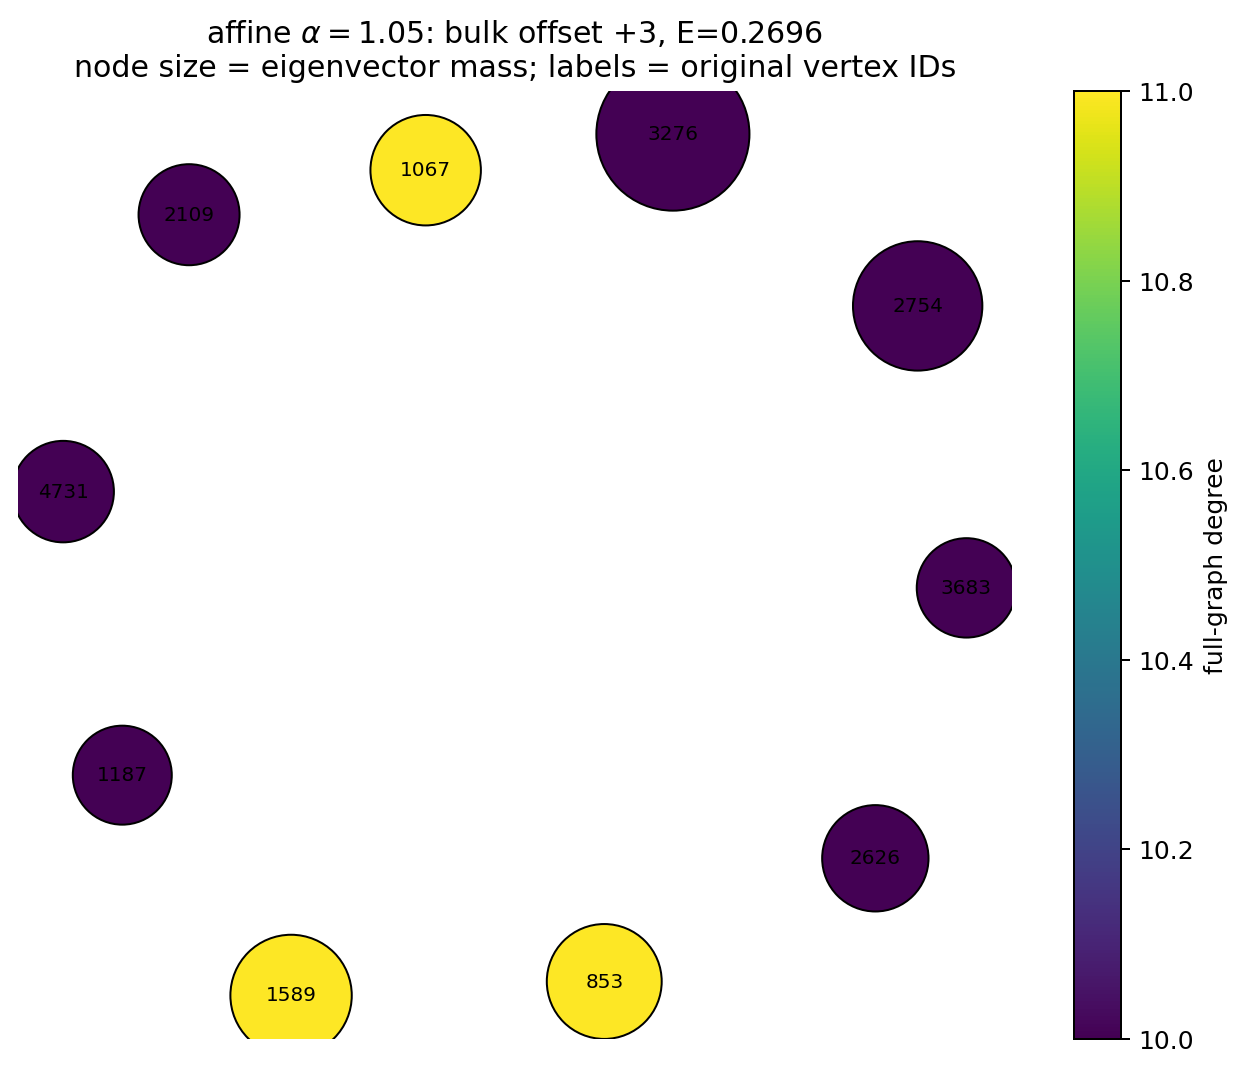
\includegraphics[width=\linewidth]{figures/affine_alpha_1p05/induced_subgraphs/bulk/bulk_offset_p003.png}
\caption*{\footnotesize bulk offset p003}\end{minipage}
\caption{Original centered bulk induced supports.}\end{figure}
\begin{figure}[H]\centering
\begin{minipage}[t]{.48\linewidth}\centering
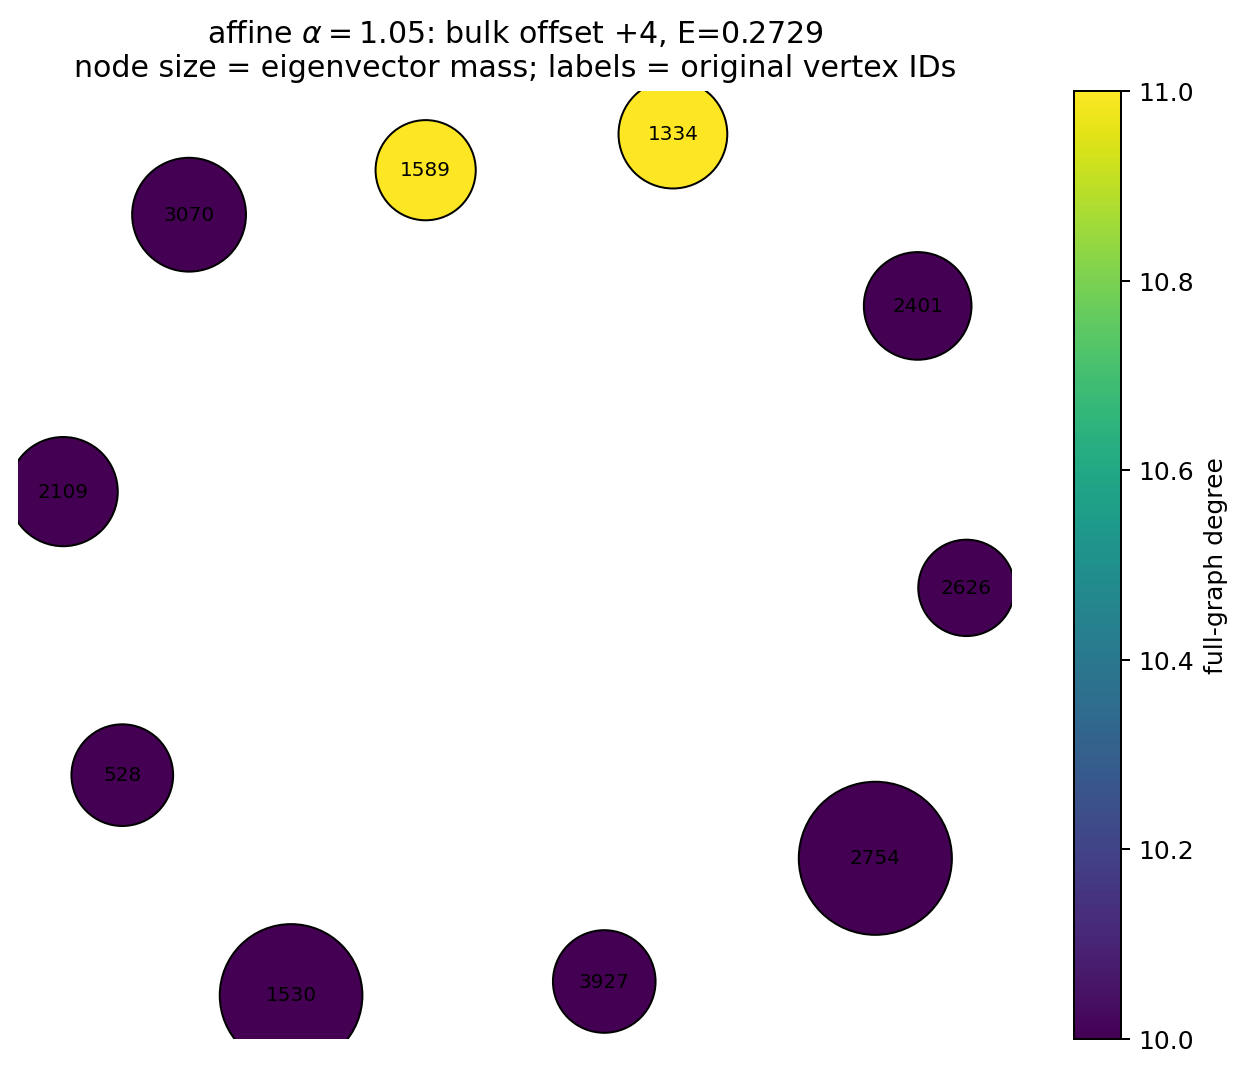
\includegraphics[width=\linewidth]{figures/affine_alpha_1p05/induced_subgraphs/bulk/bulk_offset_p004.png}
\caption*{\footnotesize bulk offset p004}\end{minipage}
\hfill
\begin{minipage}[t]{.48\linewidth}\centering
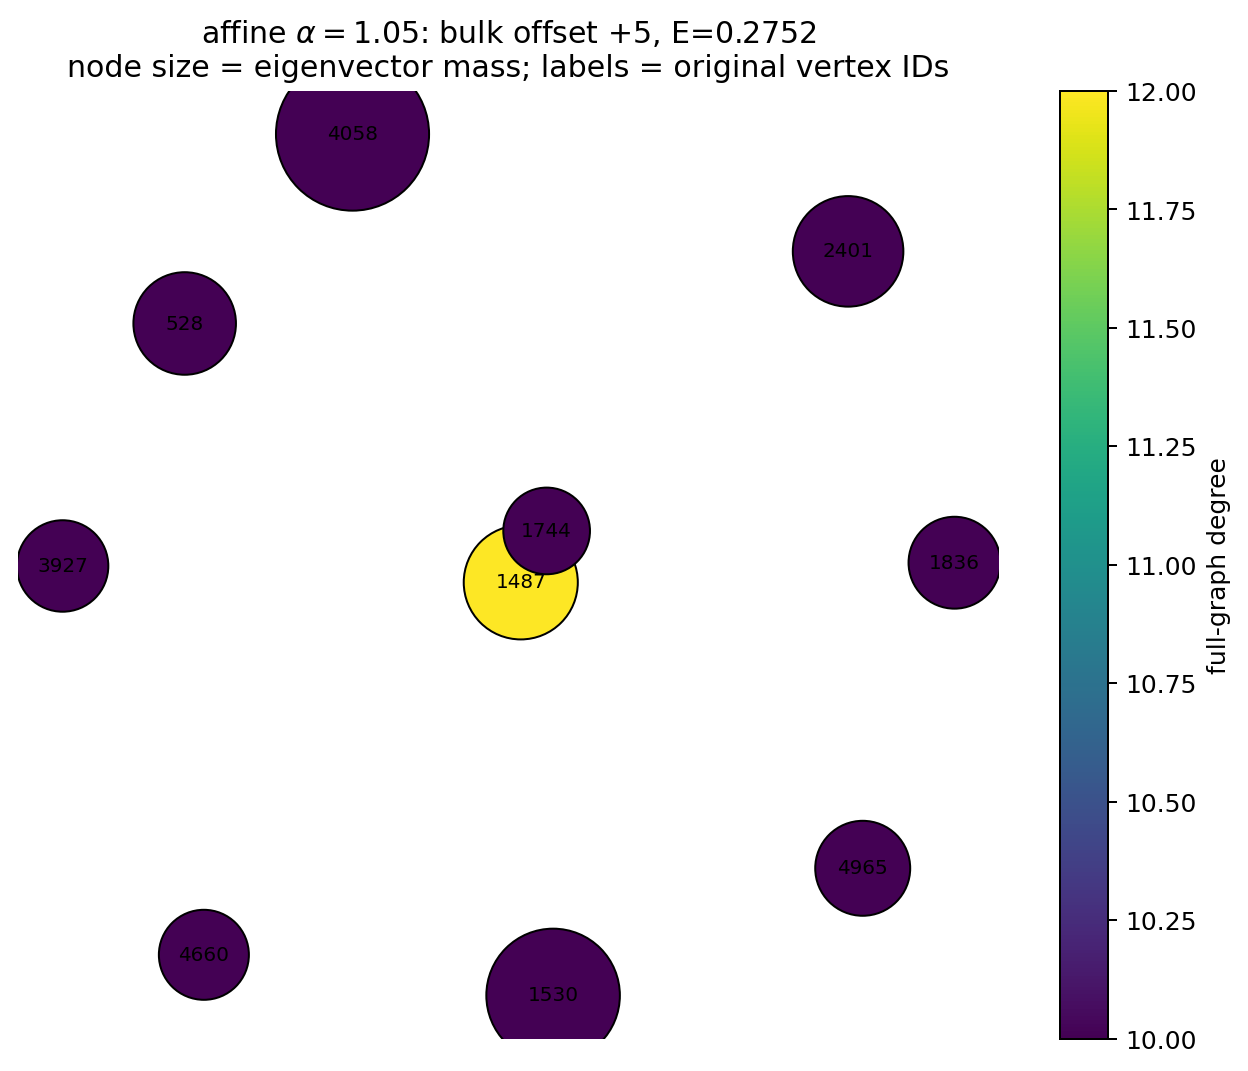
\includegraphics[width=\linewidth]{figures/affine_alpha_1p05/induced_subgraphs/bulk/bulk_offset_p005.png}
\caption*{\footnotesize bulk offset p005}\end{minipage}
\caption{Original centered bulk induced supports.}\end{figure}
\subsection{nonlinear $\zeta=1.5$: original edge ranks 1--10}
\begin{figure}[H]\centering
\begin{minipage}[t]{.48\linewidth}\centering
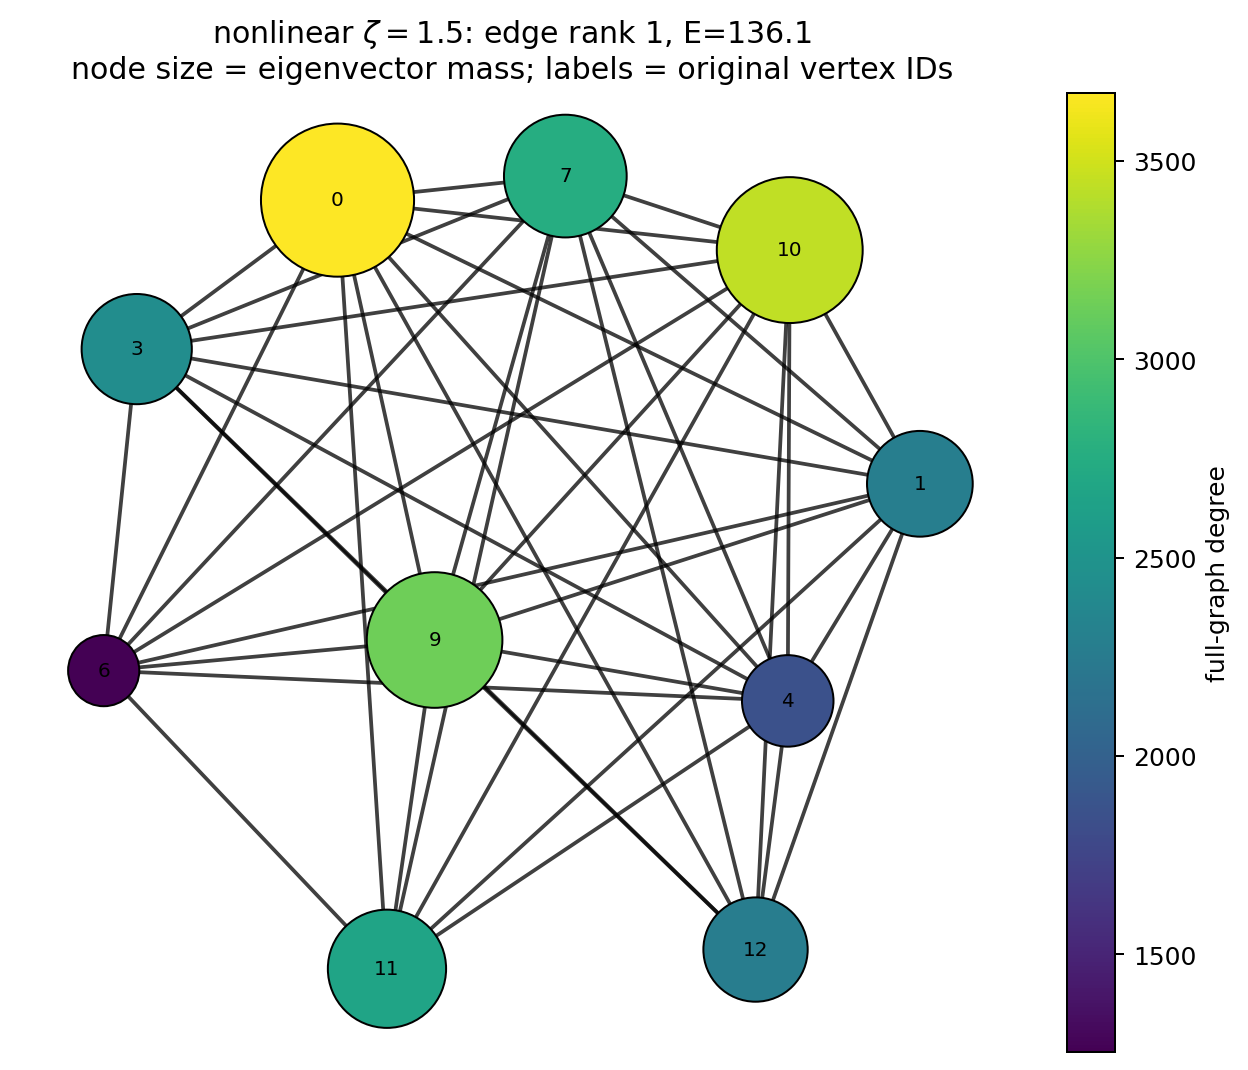
\includegraphics[width=\linewidth]{figures/nonlinear_zeta_1p5/induced_subgraphs/edge/edge_rank_001.png}
\caption*{\footnotesize edge rank 001}\end{minipage}
\hfill
\begin{minipage}[t]{.48\linewidth}\centering
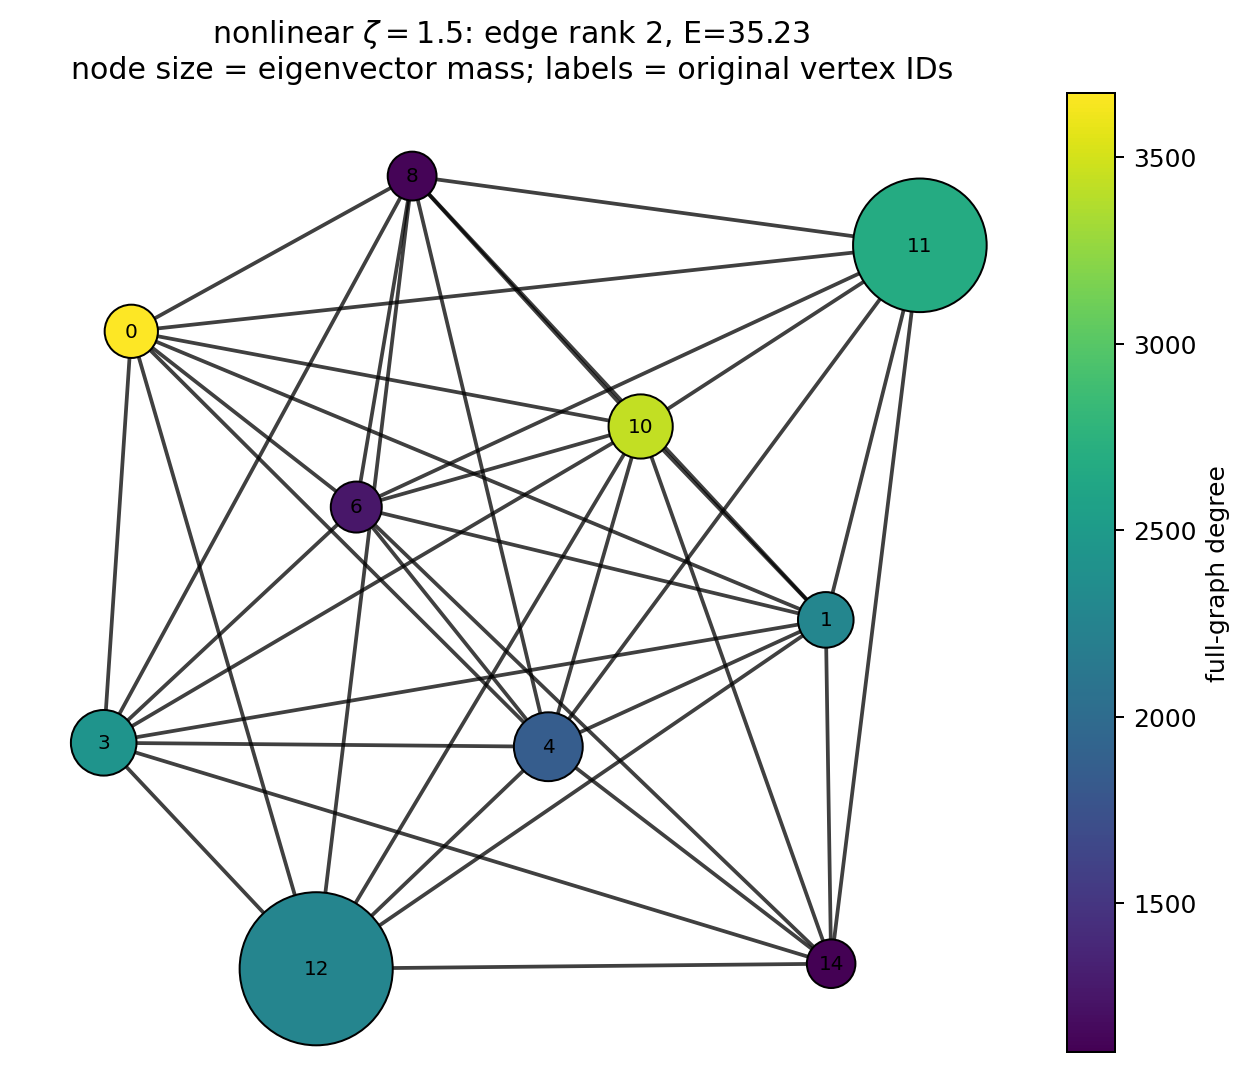
\includegraphics[width=\linewidth]{figures/nonlinear_zeta_1p5/induced_subgraphs/edge/edge_rank_002.png}
\caption*{\footnotesize edge rank 002}\end{minipage}
\par\medskip
\begin{minipage}[t]{.48\linewidth}\centering
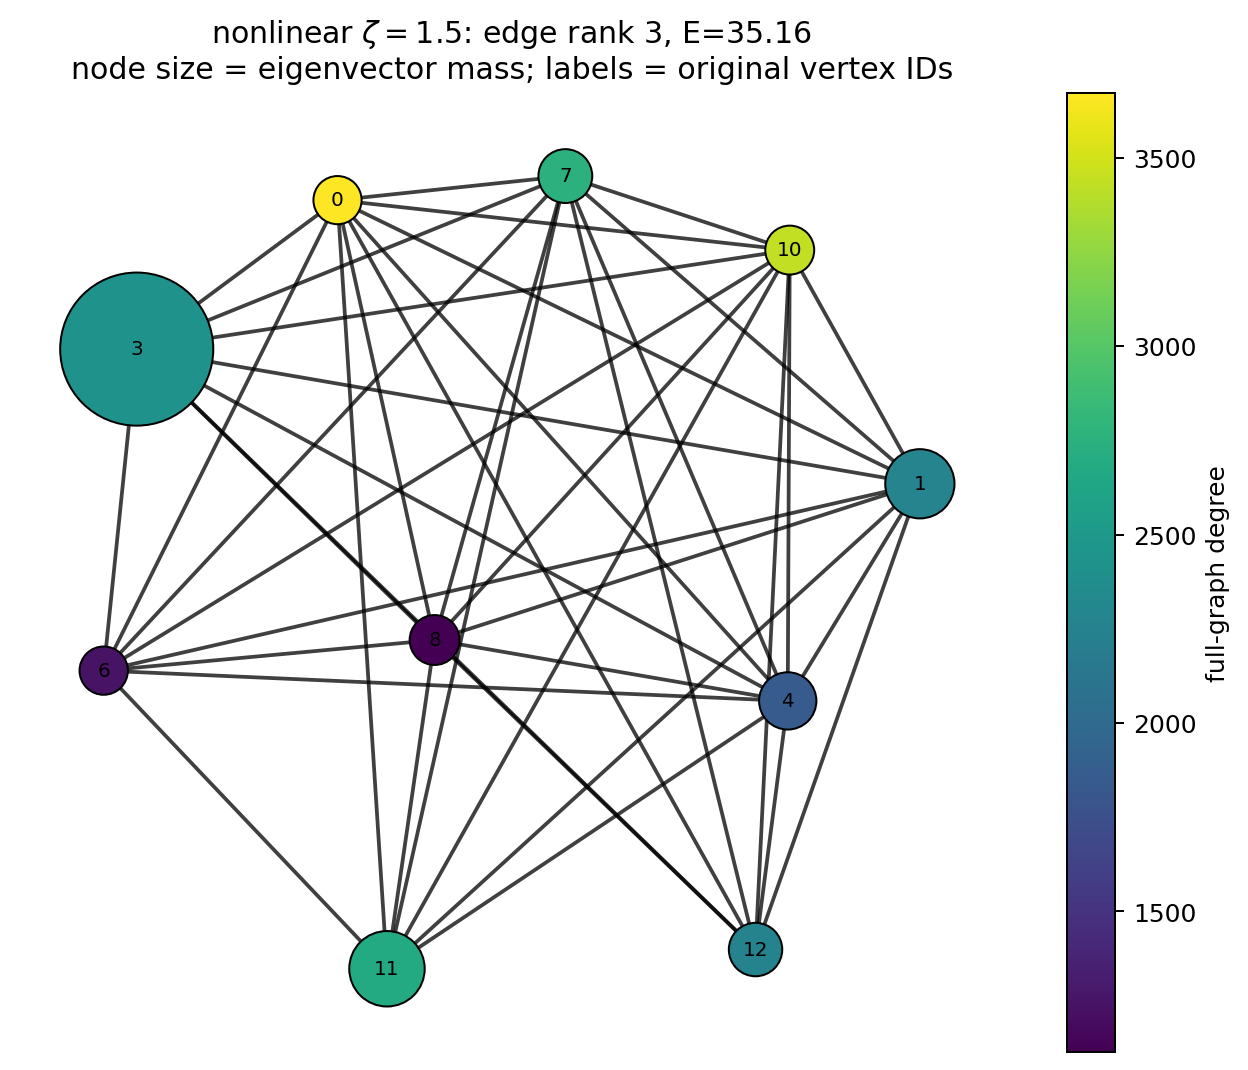
\includegraphics[width=\linewidth]{figures/nonlinear_zeta_1p5/induced_subgraphs/edge/edge_rank_003.png}
\caption*{\footnotesize edge rank 003}\end{minipage}
\hfill
\begin{minipage}[t]{.48\linewidth}\centering
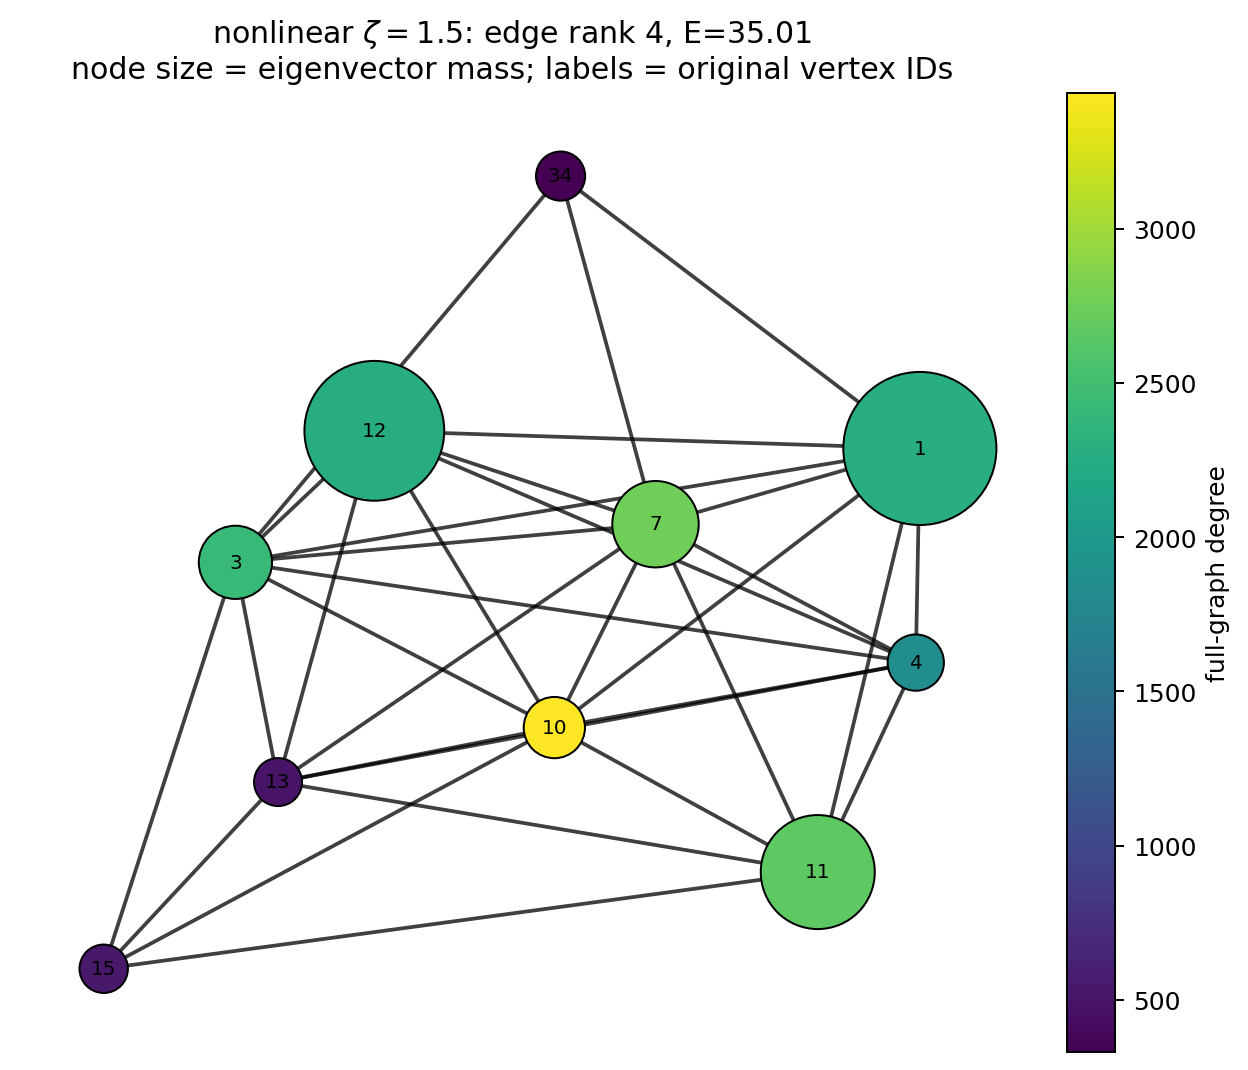
\includegraphics[width=\linewidth]{figures/nonlinear_zeta_1p5/induced_subgraphs/edge/edge_rank_004.png}
\caption*{\footnotesize edge rank 004}\end{minipage}
\caption{Original edge induced supports, ranks 1--4.}\end{figure}
\begin{figure}[H]\centering
\begin{minipage}[t]{.48\linewidth}\centering
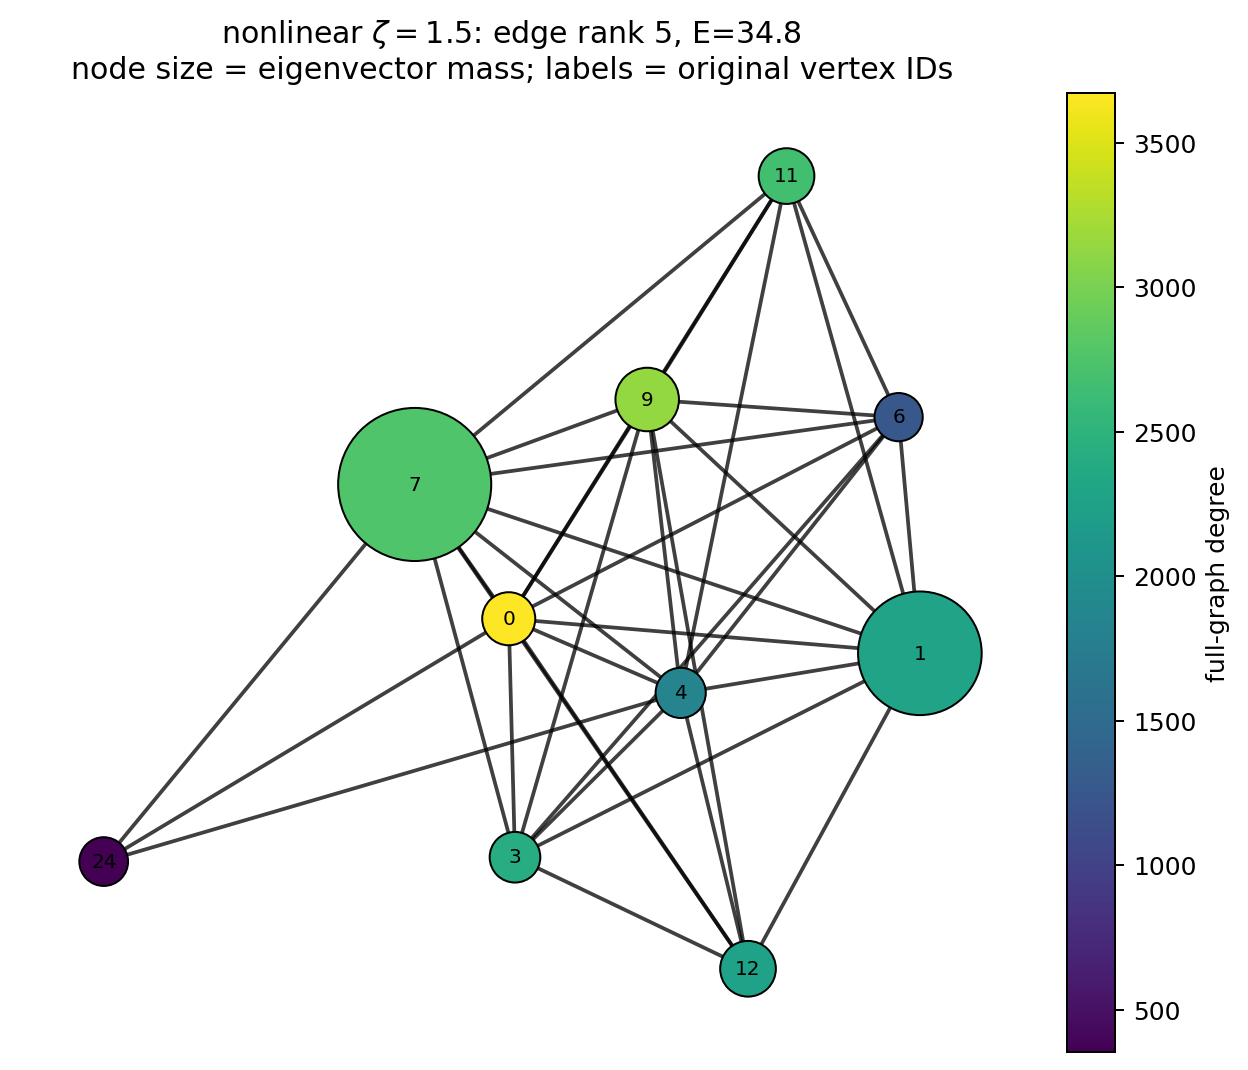
\includegraphics[width=\linewidth]{figures/nonlinear_zeta_1p5/induced_subgraphs/edge/edge_rank_005.png}
\caption*{\footnotesize edge rank 005}\end{minipage}
\hfill
\begin{minipage}[t]{.48\linewidth}\centering
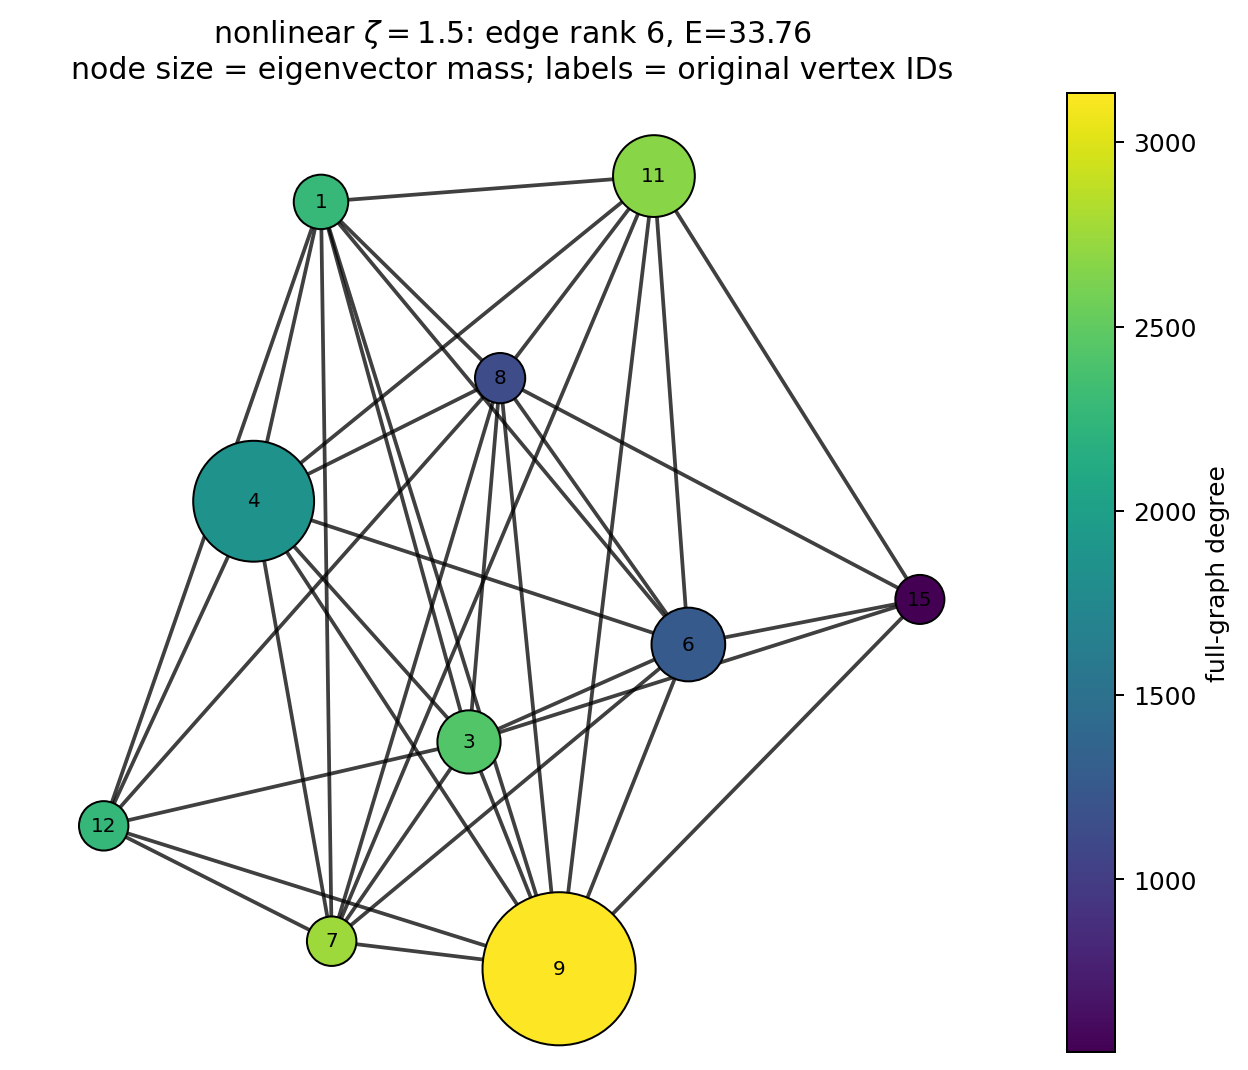
\includegraphics[width=\linewidth]{figures/nonlinear_zeta_1p5/induced_subgraphs/edge/edge_rank_006.png}
\caption*{\footnotesize edge rank 006}\end{minipage}
\par\medskip
\begin{minipage}[t]{.48\linewidth}\centering
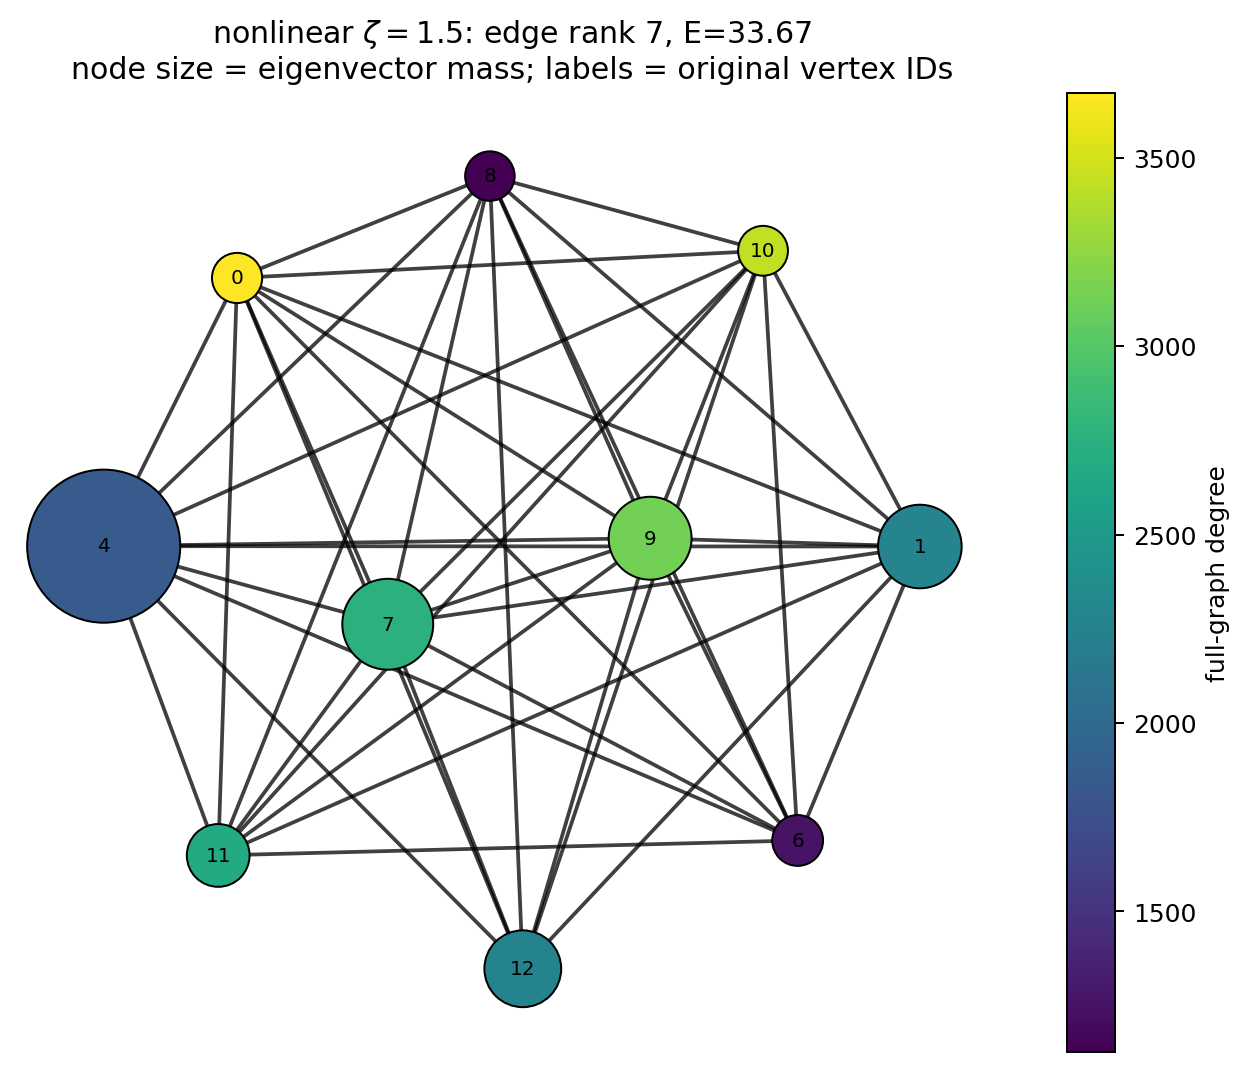
\includegraphics[width=\linewidth]{figures/nonlinear_zeta_1p5/induced_subgraphs/edge/edge_rank_007.png}
\caption*{\footnotesize edge rank 007}\end{minipage}
\hfill
\begin{minipage}[t]{.48\linewidth}\centering
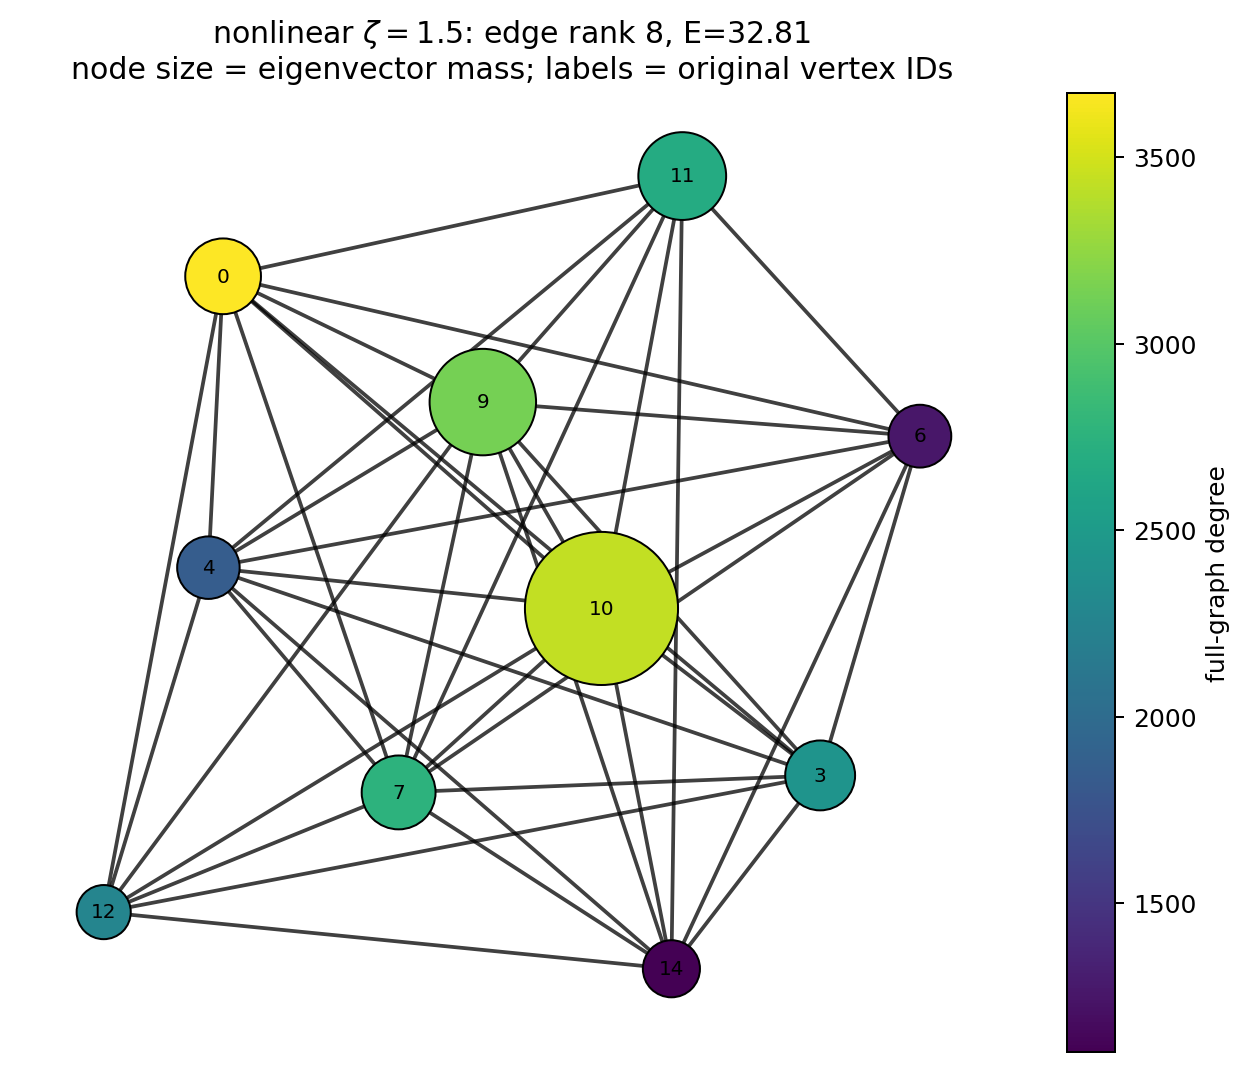
\includegraphics[width=\linewidth]{figures/nonlinear_zeta_1p5/induced_subgraphs/edge/edge_rank_008.png}
\caption*{\footnotesize edge rank 008}\end{minipage}
\caption{Original edge induced supports, ranks 5--8.}\end{figure}
\begin{figure}[H]\centering
\begin{minipage}[t]{.48\linewidth}\centering
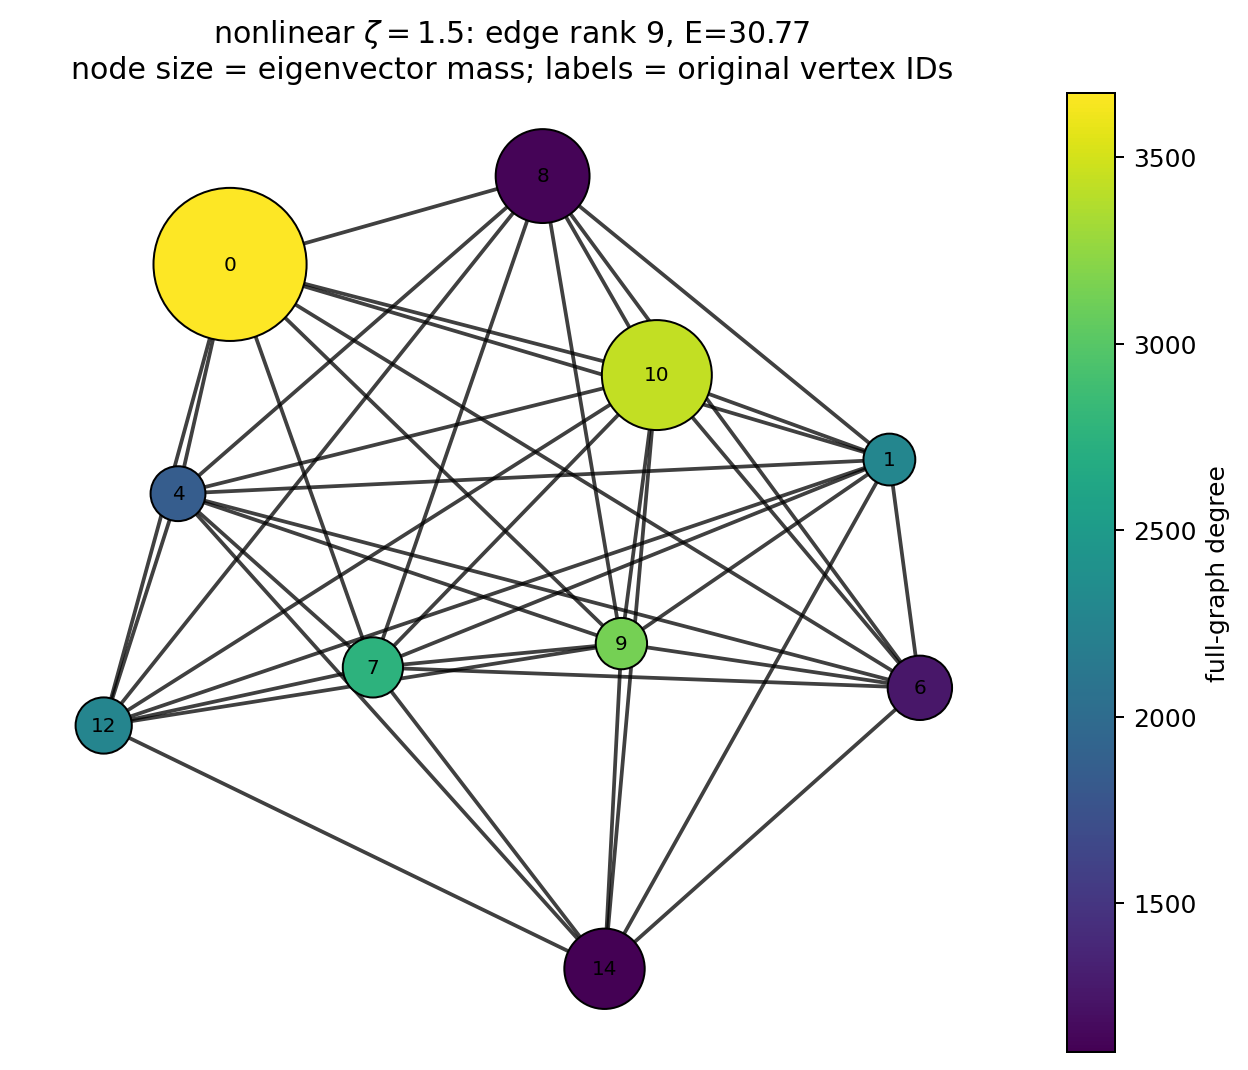
\includegraphics[width=\linewidth]{figures/nonlinear_zeta_1p5/induced_subgraphs/edge/edge_rank_009.png}
\caption*{\footnotesize edge rank 009}\end{minipage}
\hfill
\begin{minipage}[t]{.48\linewidth}\centering
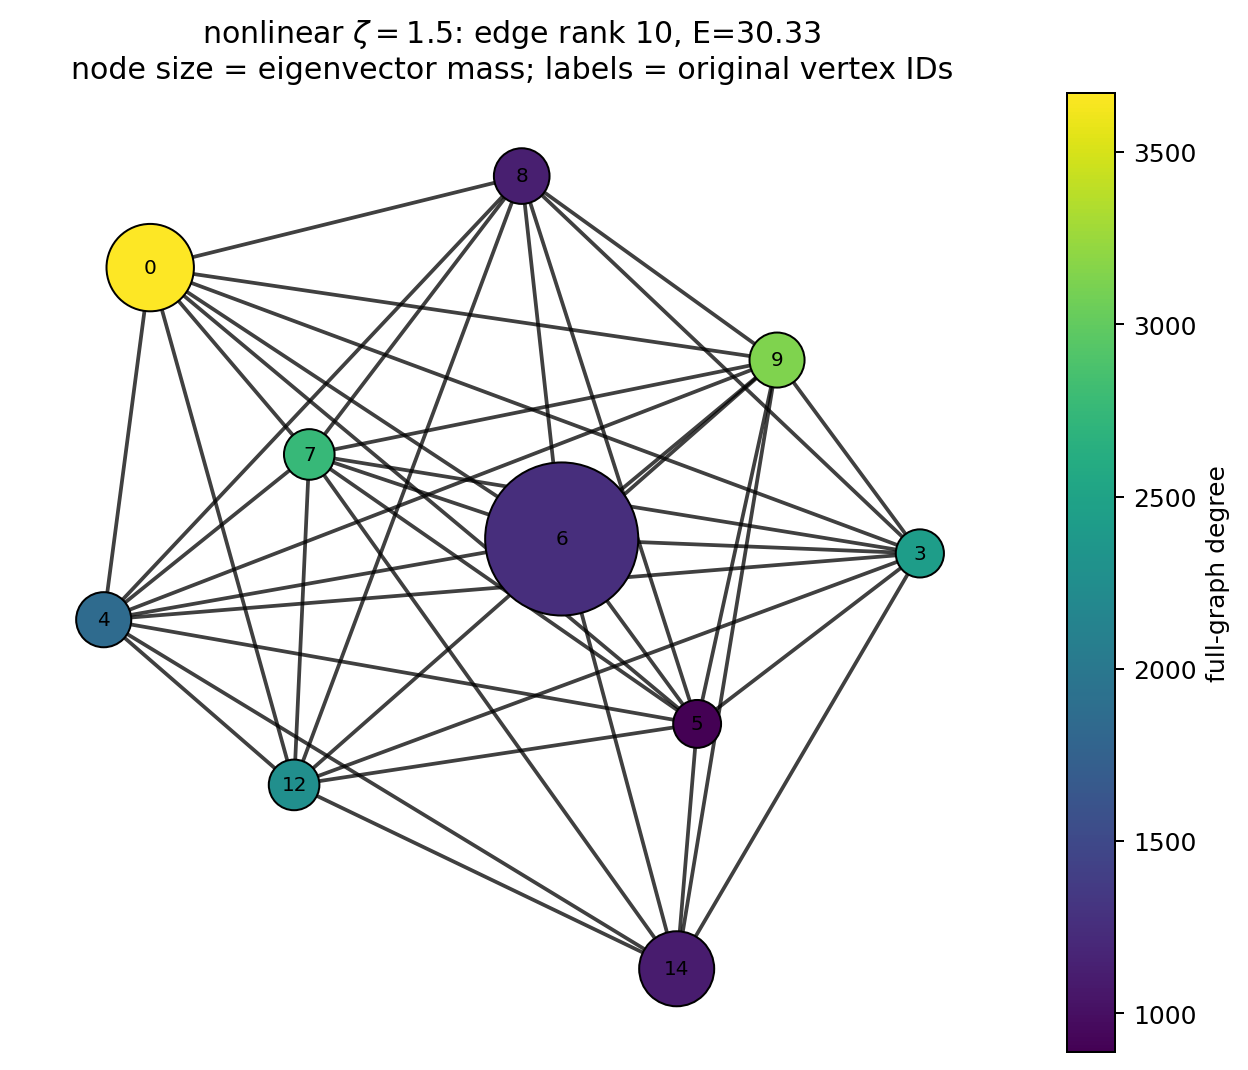
\includegraphics[width=\linewidth]{figures/nonlinear_zeta_1p5/induced_subgraphs/edge/edge_rank_010.png}
\caption*{\footnotesize edge rank 010}\end{minipage}
\caption{Original edge induced supports, ranks 9--10.}\end{figure}
\subsection{nonlinear $\zeta=1.5$: original centered bulk window}
\begin{figure}[H]\centering
\begin{minipage}[t]{.48\linewidth}\centering
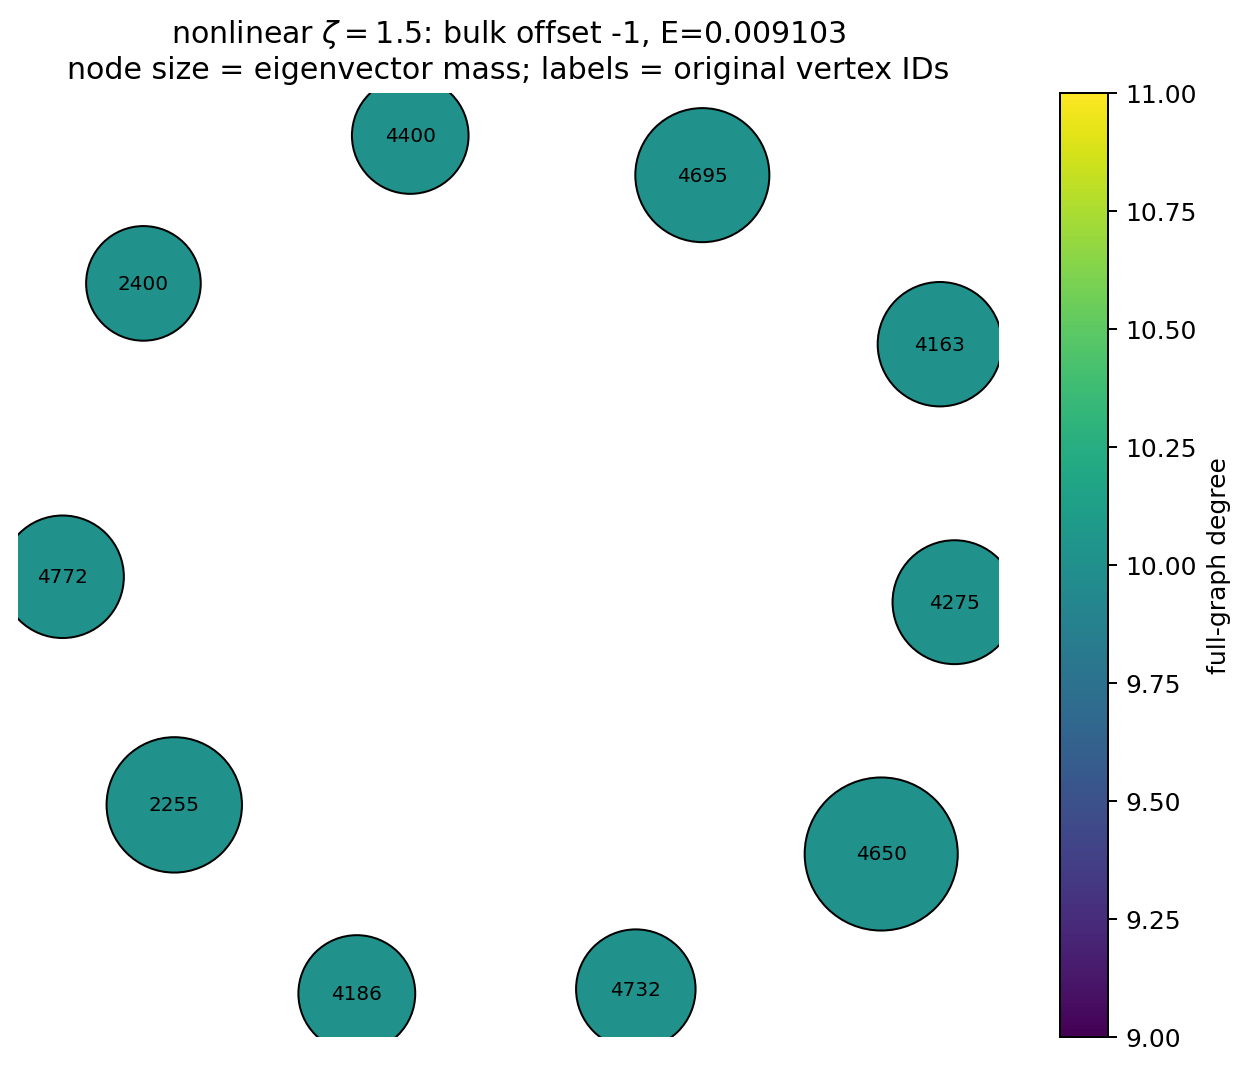
\includegraphics[width=\linewidth]{figures/nonlinear_zeta_1p5/induced_subgraphs/bulk/bulk_offset_m001.png}
\caption*{\footnotesize bulk offset m001}\end{minipage}
\hfill
\begin{minipage}[t]{.48\linewidth}\centering
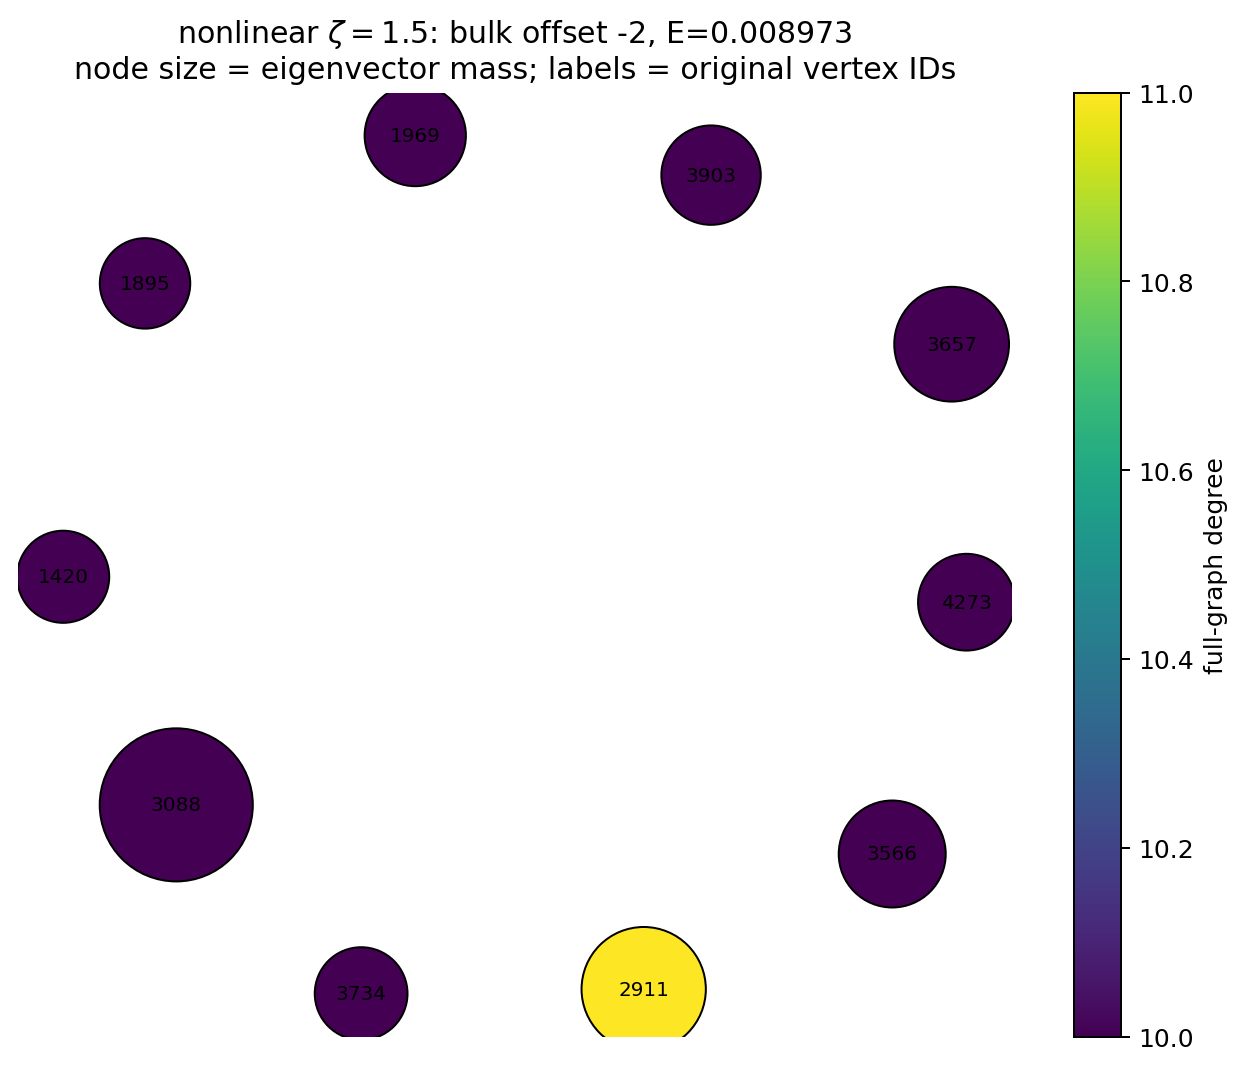
\includegraphics[width=\linewidth]{figures/nonlinear_zeta_1p5/induced_subgraphs/bulk/bulk_offset_m002.png}
\caption*{\footnotesize bulk offset m002}\end{minipage}
\par\medskip
\begin{minipage}[t]{.48\linewidth}\centering
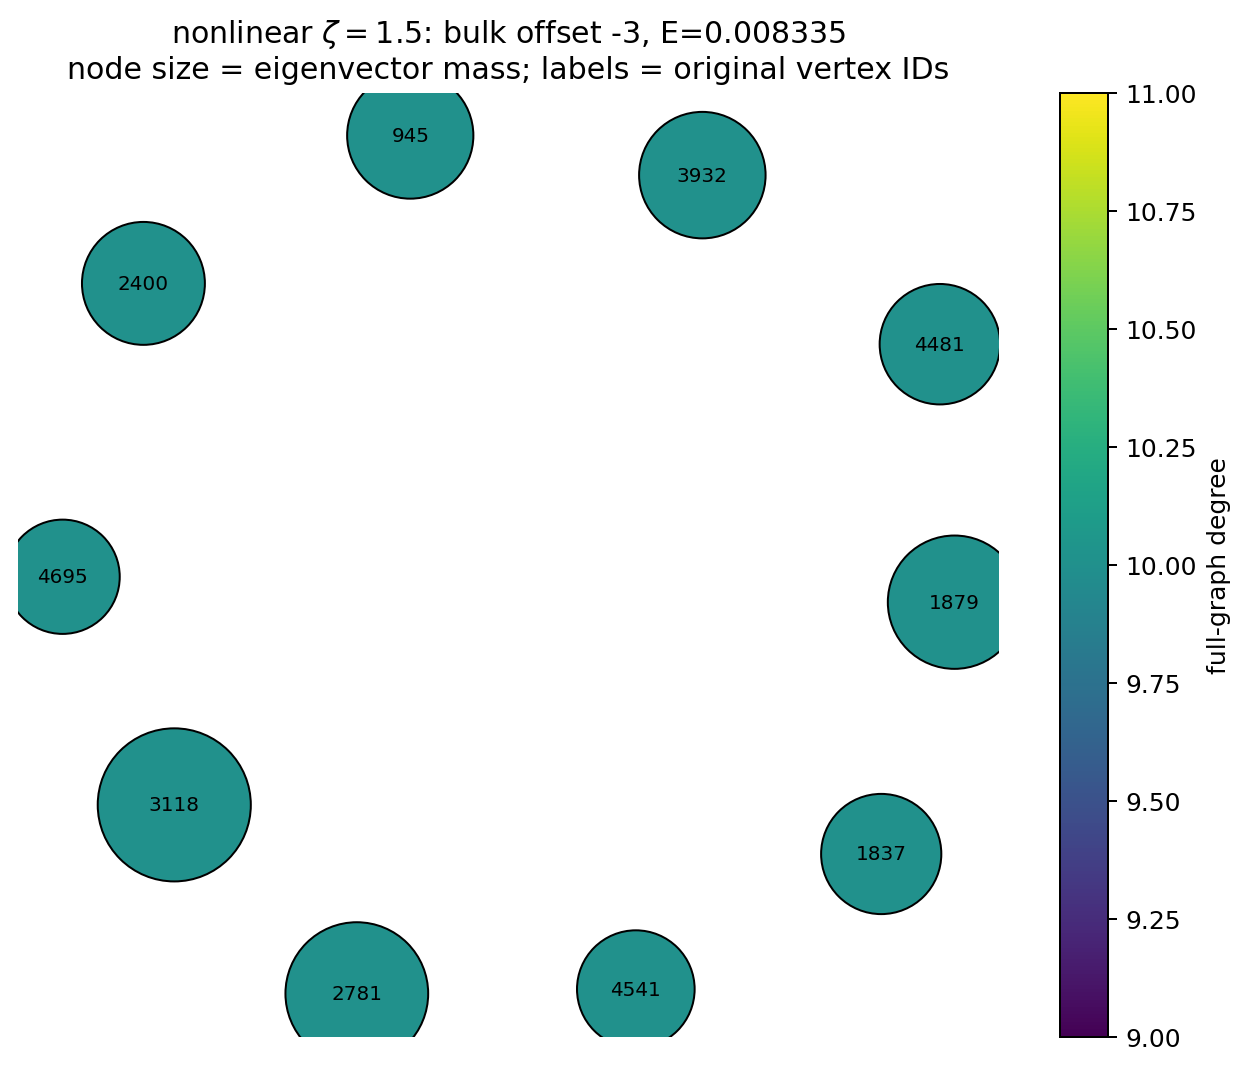
\includegraphics[width=\linewidth]{figures/nonlinear_zeta_1p5/induced_subgraphs/bulk/bulk_offset_m003.png}
\caption*{\footnotesize bulk offset m003}\end{minipage}
\hfill
\begin{minipage}[t]{.48\linewidth}\centering
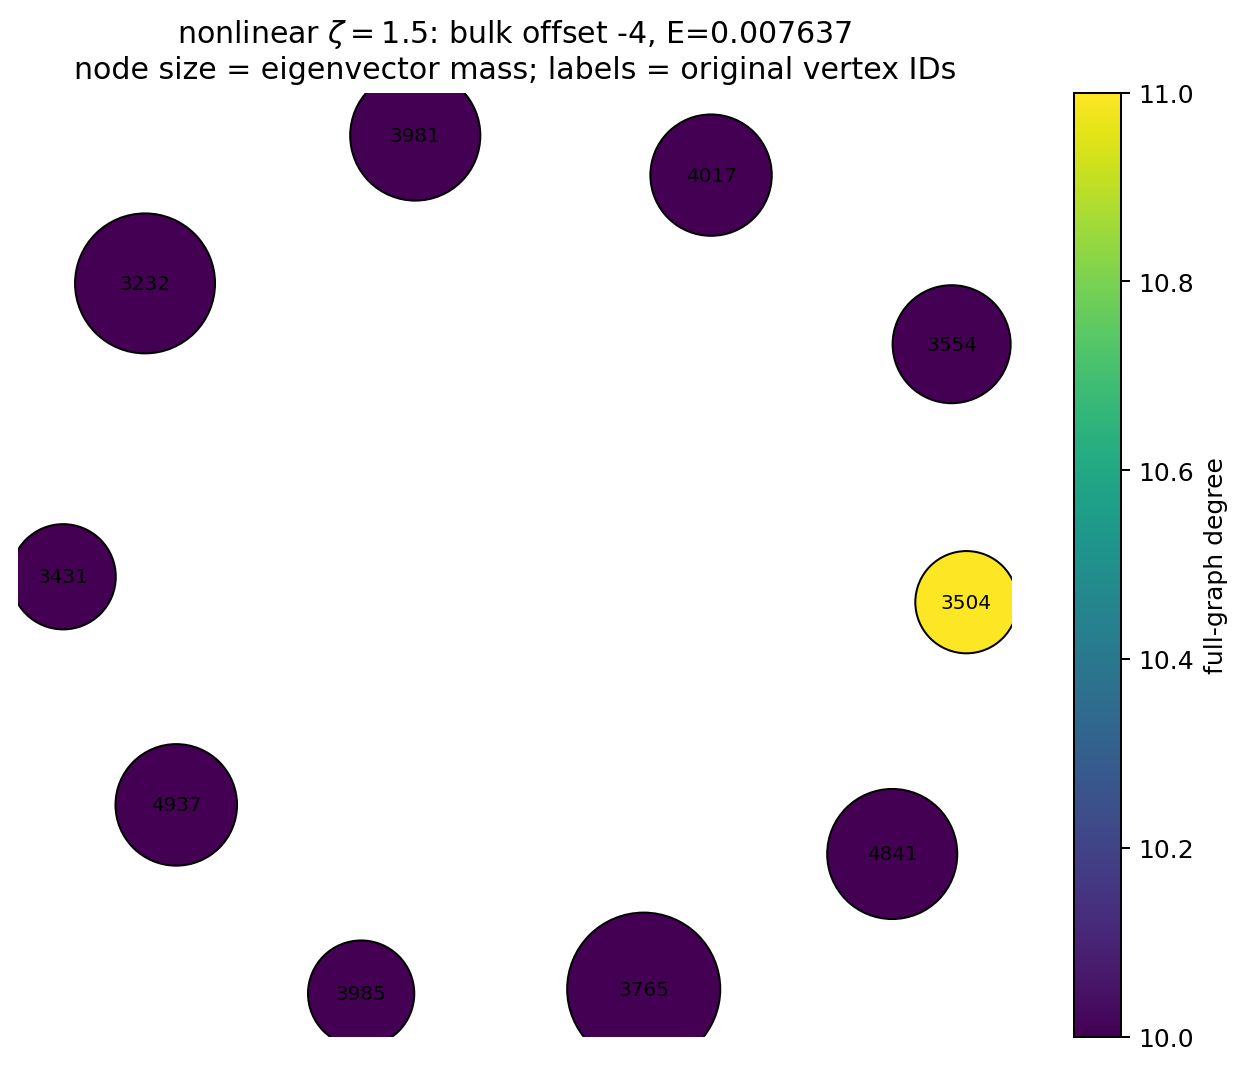
\includegraphics[width=\linewidth]{figures/nonlinear_zeta_1p5/induced_subgraphs/bulk/bulk_offset_m004.png}
\caption*{\footnotesize bulk offset m004}\end{minipage}
\caption{Original centered bulk induced supports.}\end{figure}
\begin{figure}[H]\centering
\begin{minipage}[t]{.48\linewidth}\centering
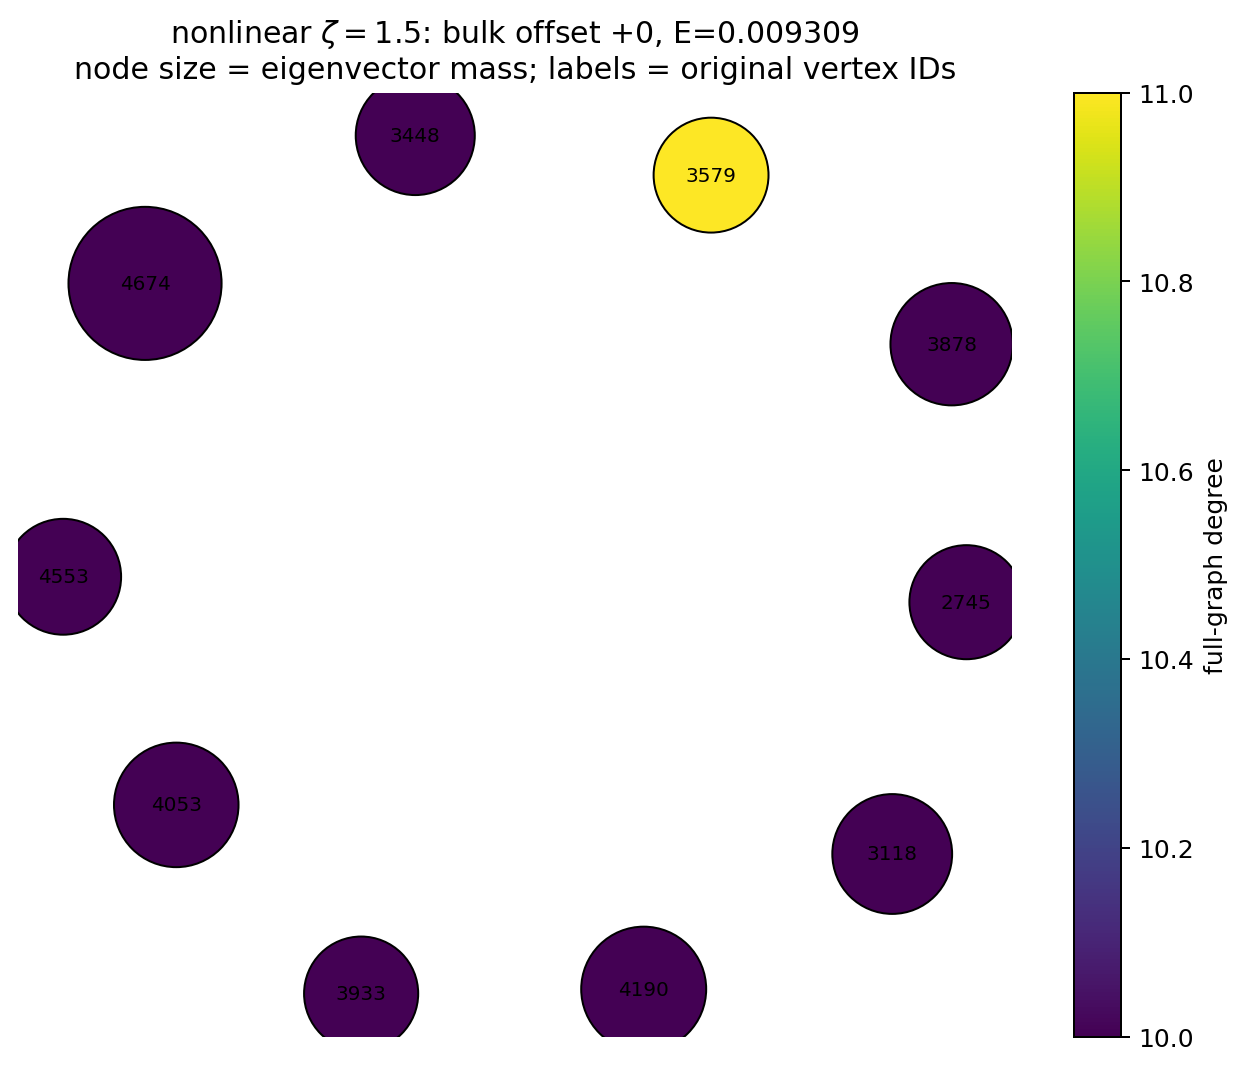
\includegraphics[width=\linewidth]{figures/nonlinear_zeta_1p5/induced_subgraphs/bulk/bulk_offset_p000.png}
\caption*{\footnotesize bulk offset p000}\end{minipage}
\hfill
\begin{minipage}[t]{.48\linewidth}\centering
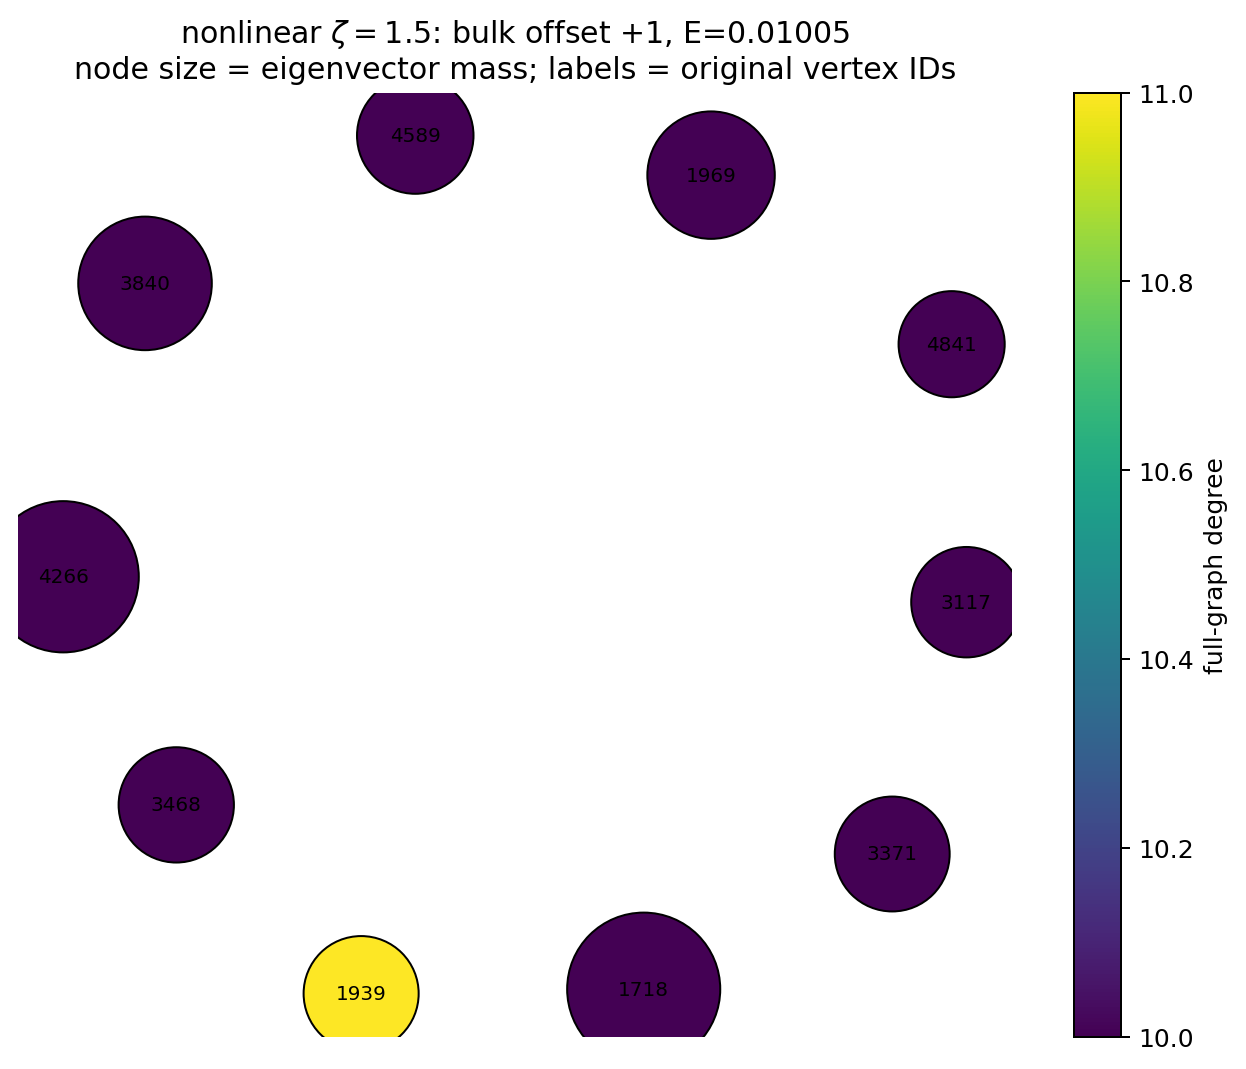
\includegraphics[width=\linewidth]{figures/nonlinear_zeta_1p5/induced_subgraphs/bulk/bulk_offset_p001.png}
\caption*{\footnotesize bulk offset p001}\end{minipage}
\par\medskip
\begin{minipage}[t]{.48\linewidth}\centering
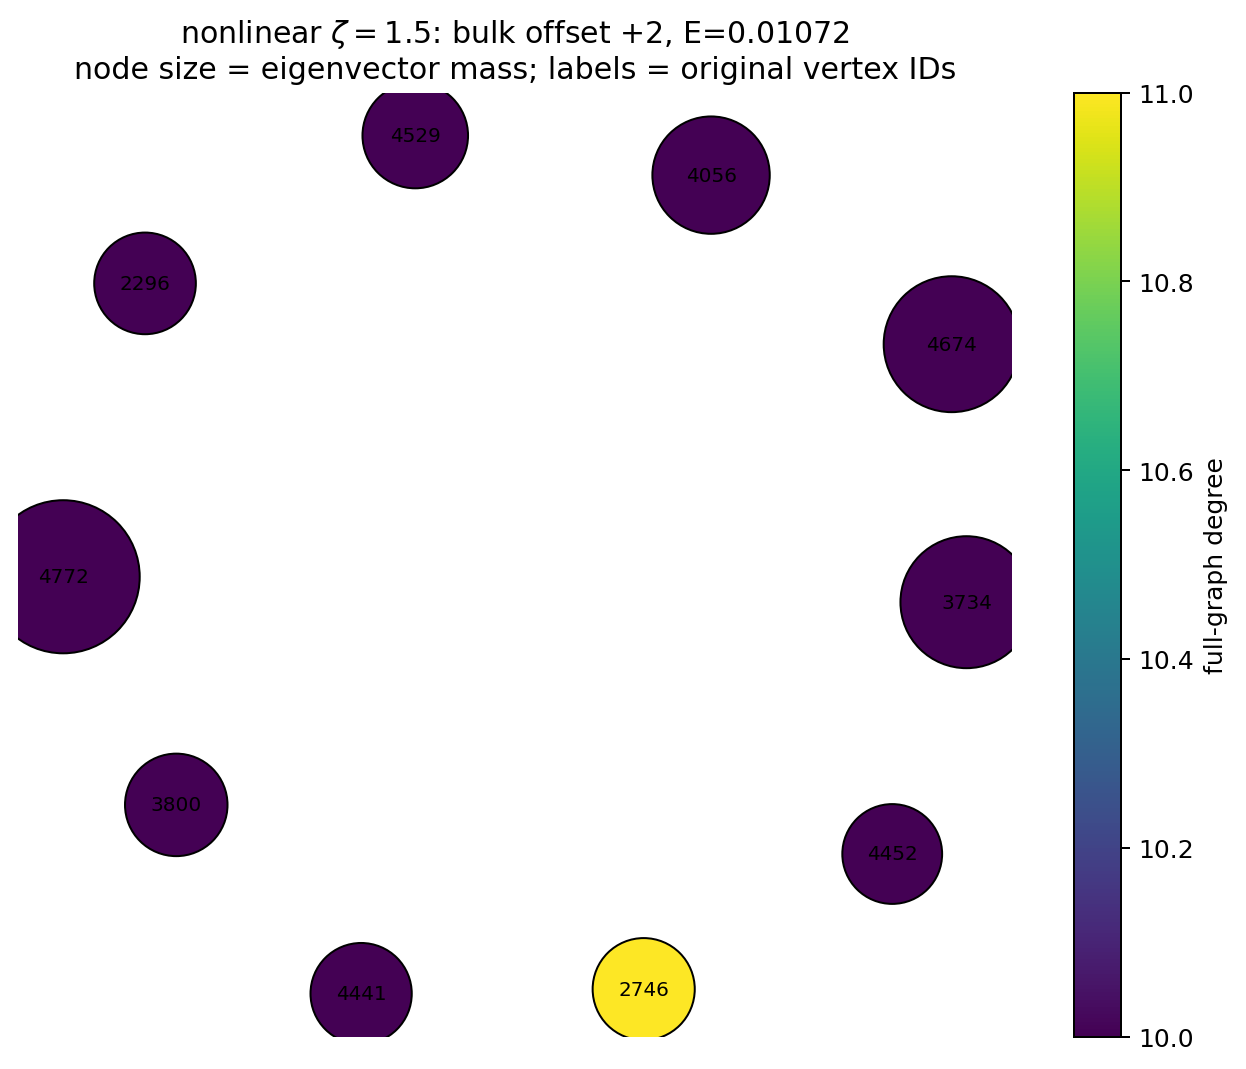
\includegraphics[width=\linewidth]{figures/nonlinear_zeta_1p5/induced_subgraphs/bulk/bulk_offset_p002.png}
\caption*{\footnotesize bulk offset p002}\end{minipage}
\hfill
\begin{minipage}[t]{.48\linewidth}\centering
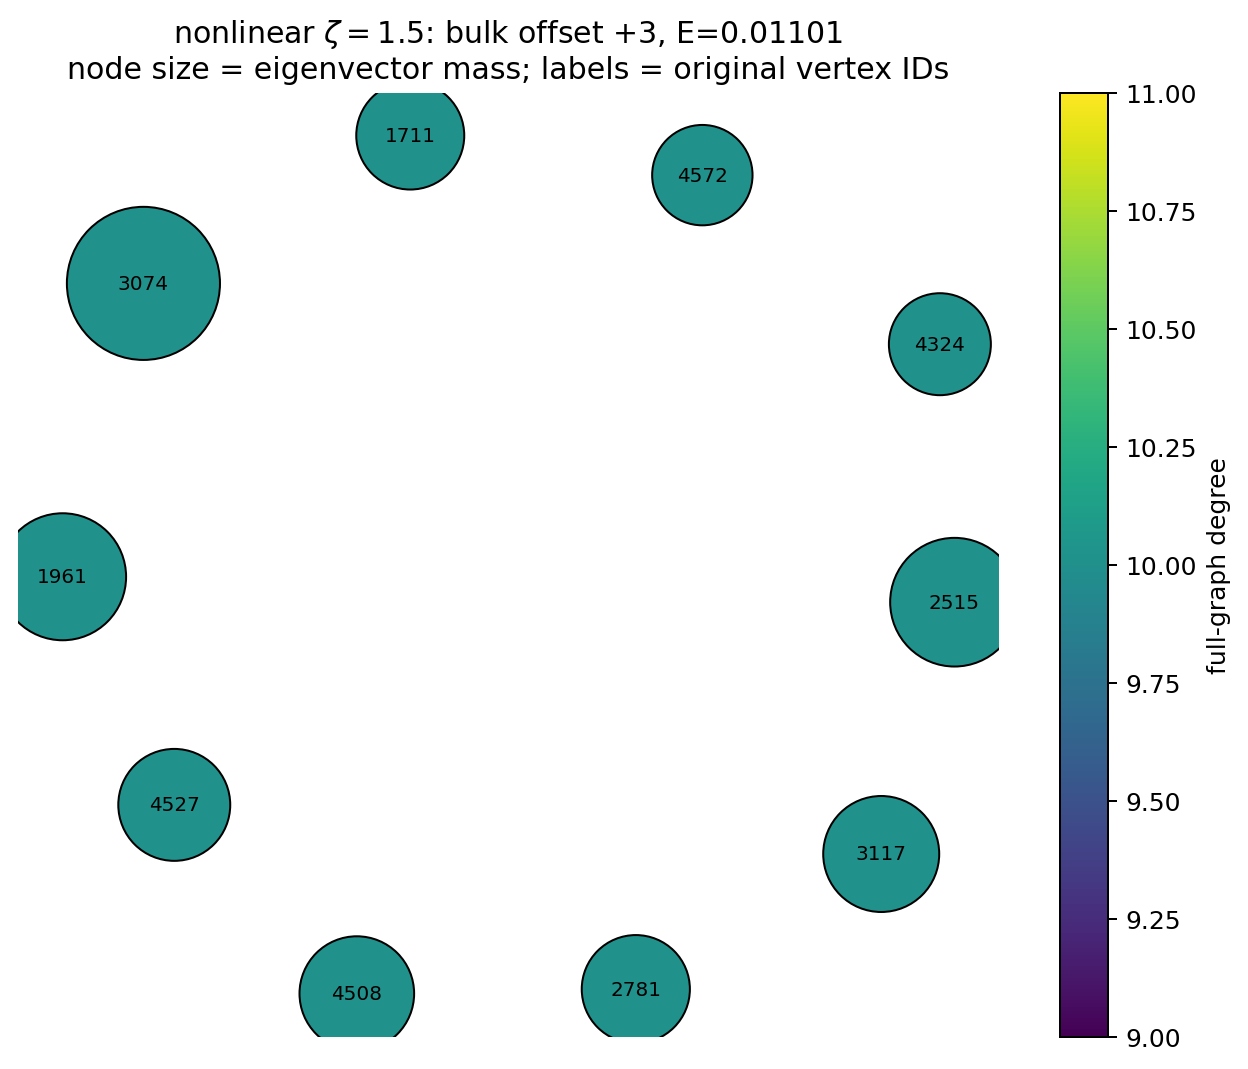
\includegraphics[width=\linewidth]{figures/nonlinear_zeta_1p5/induced_subgraphs/bulk/bulk_offset_p003.png}
\caption*{\footnotesize bulk offset p003}\end{minipage}
\caption{Original centered bulk induced supports.}\end{figure}
\begin{figure}[H]\centering
\begin{minipage}[t]{.48\linewidth}\centering
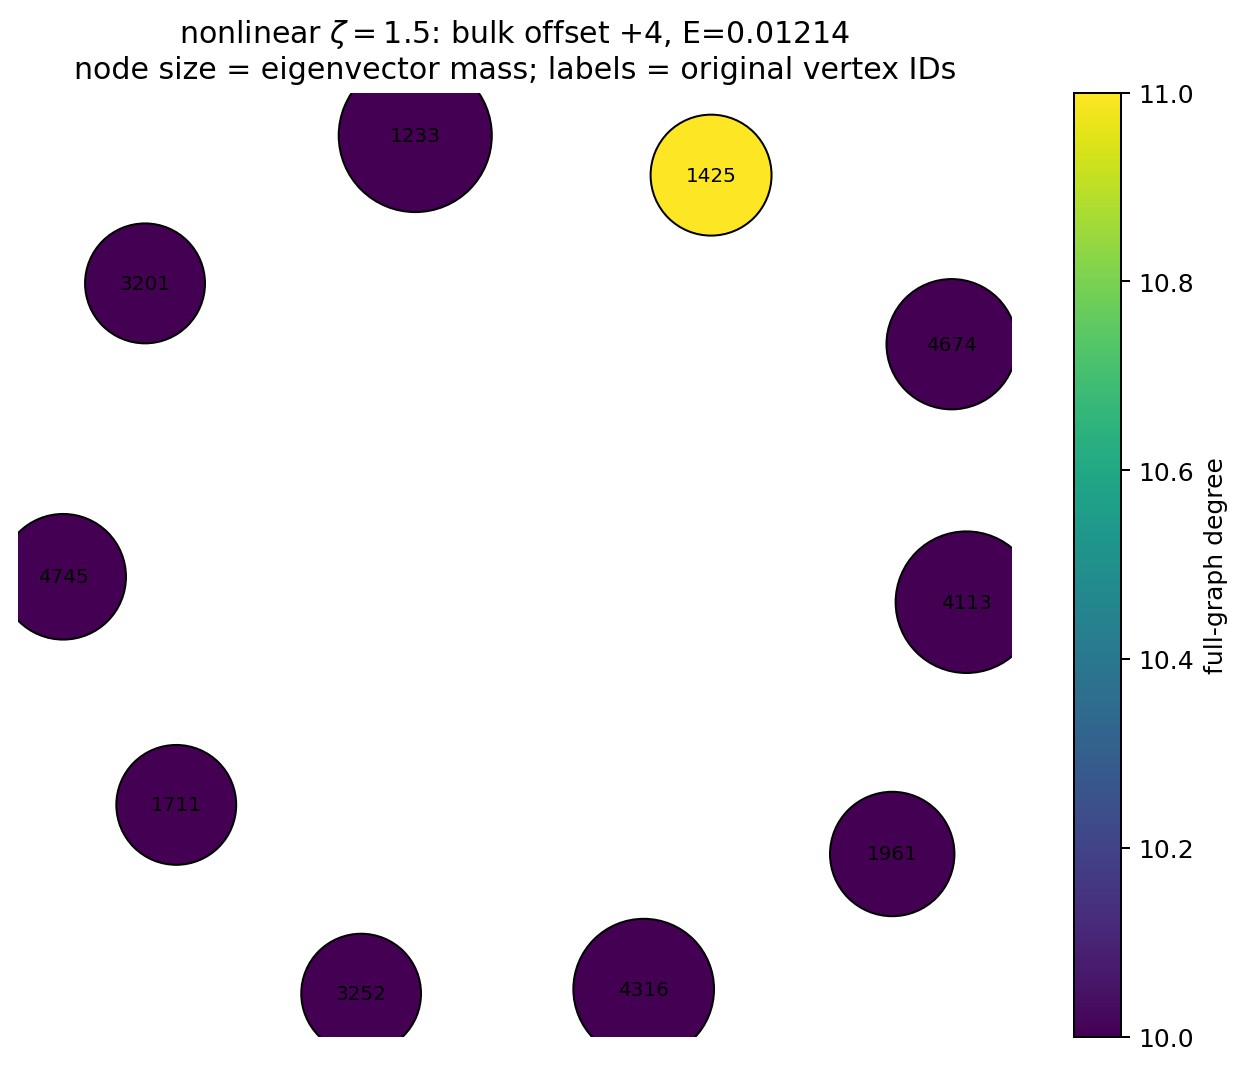
\includegraphics[width=\linewidth]{figures/nonlinear_zeta_1p5/induced_subgraphs/bulk/bulk_offset_p004.png}
\caption*{\footnotesize bulk offset p004}\end{minipage}
\hfill
\begin{minipage}[t]{.48\linewidth}\centering
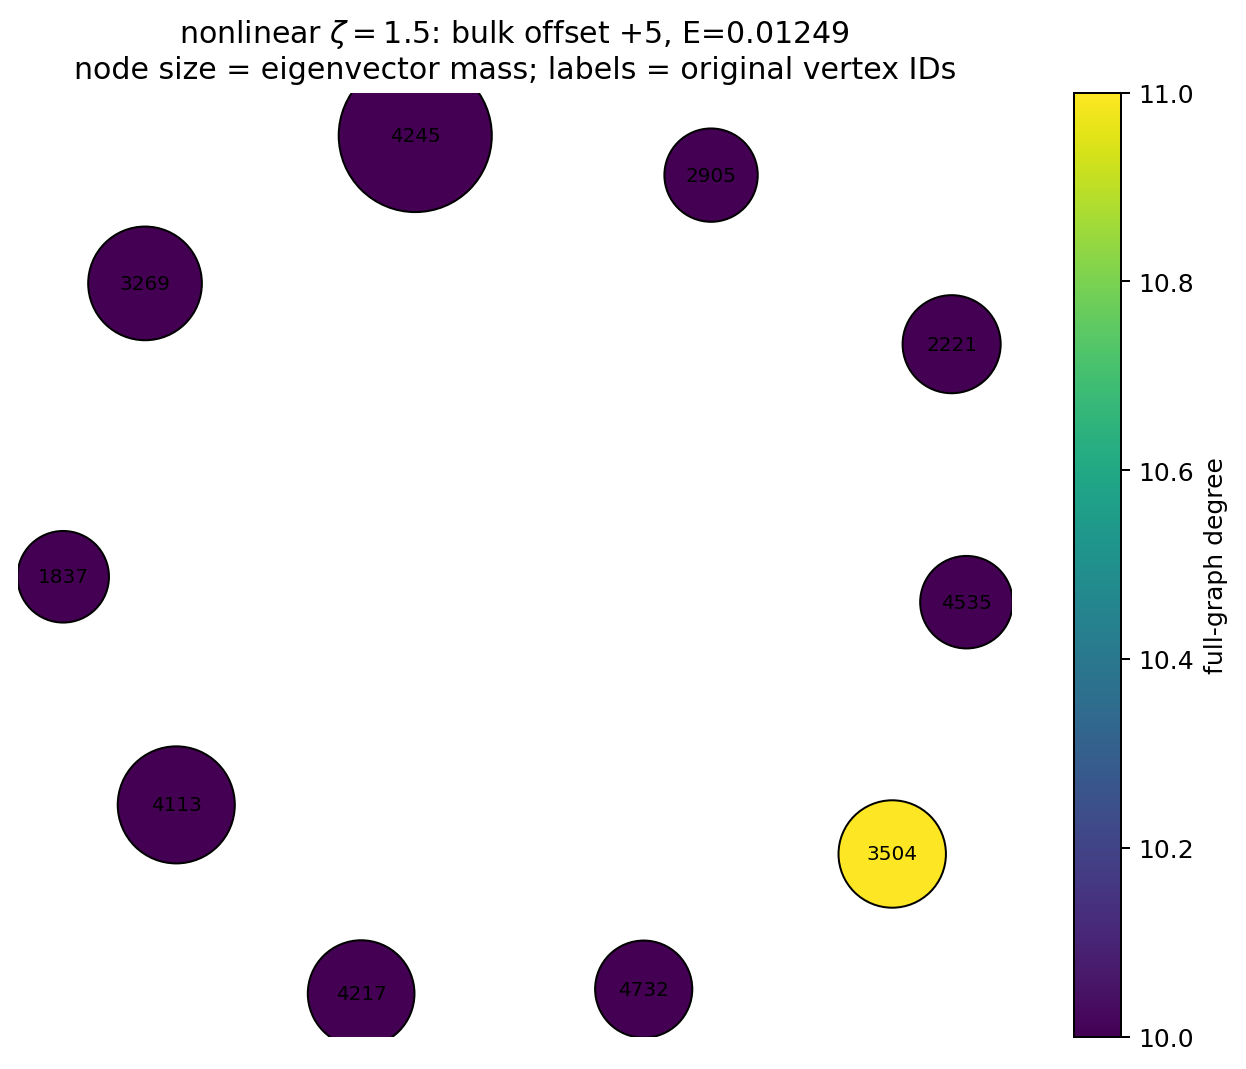
\includegraphics[width=\linewidth]{figures/nonlinear_zeta_1p5/induced_subgraphs/bulk/bulk_offset_p005.png}
\caption*{\footnotesize bulk offset p005}\end{minipage}
\caption{Original centered bulk induced supports.}\end{figure}
\subsection{affine $\alpha=2.0$: original edge ranks 1--10}
\begin{figure}[H]\centering
\begin{minipage}[t]{.48\linewidth}\centering
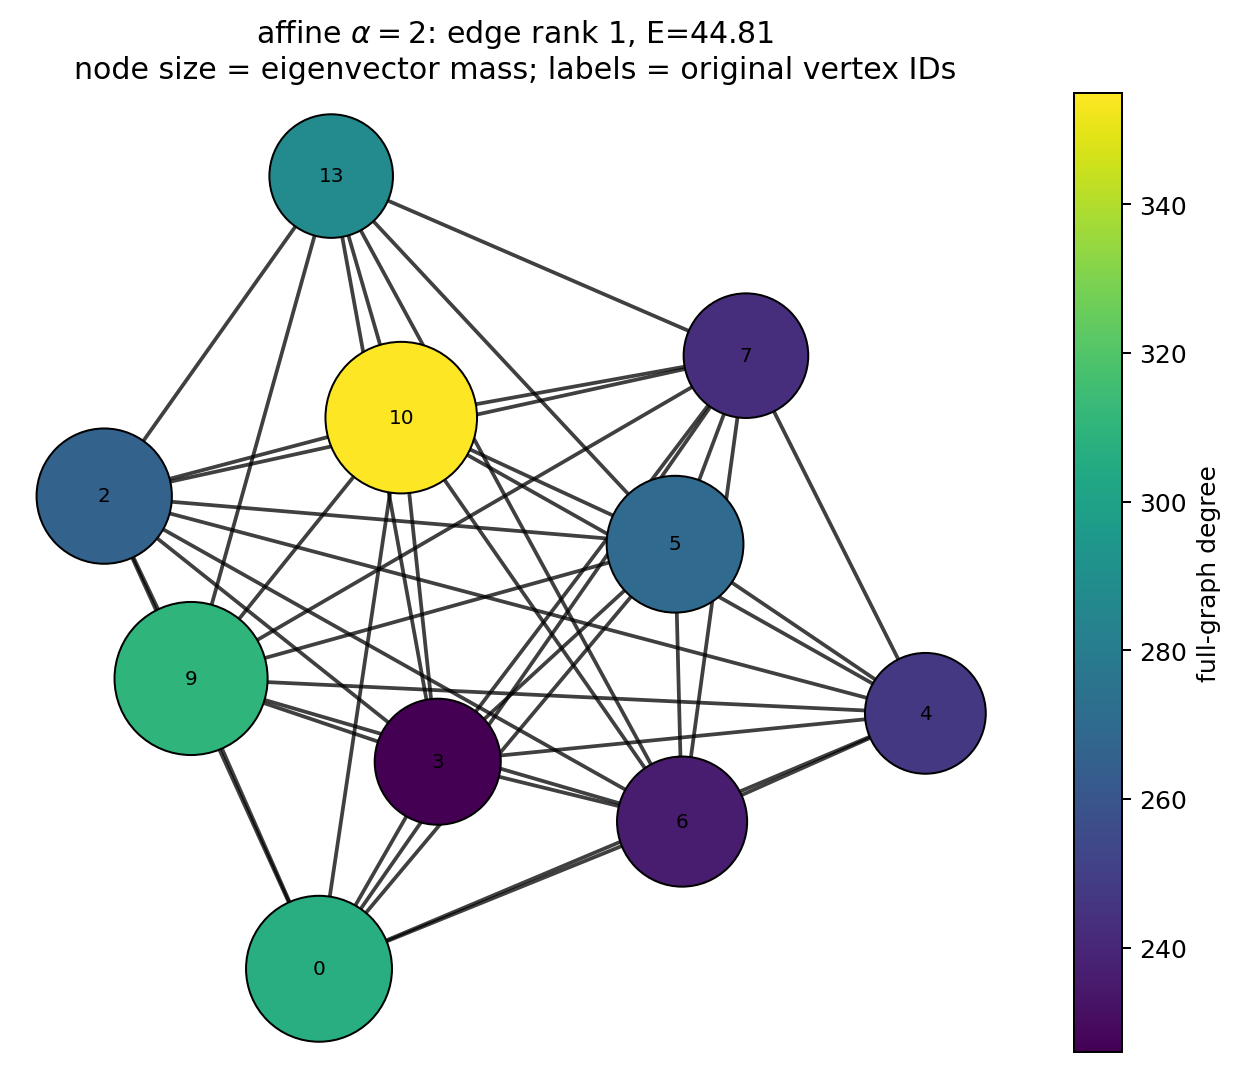
\includegraphics[width=\linewidth]{figures/affine_alpha_2p0/induced_subgraphs/edge/edge_rank_001.png}
\caption*{\footnotesize edge rank 001}\end{minipage}
\hfill
\begin{minipage}[t]{.48\linewidth}\centering
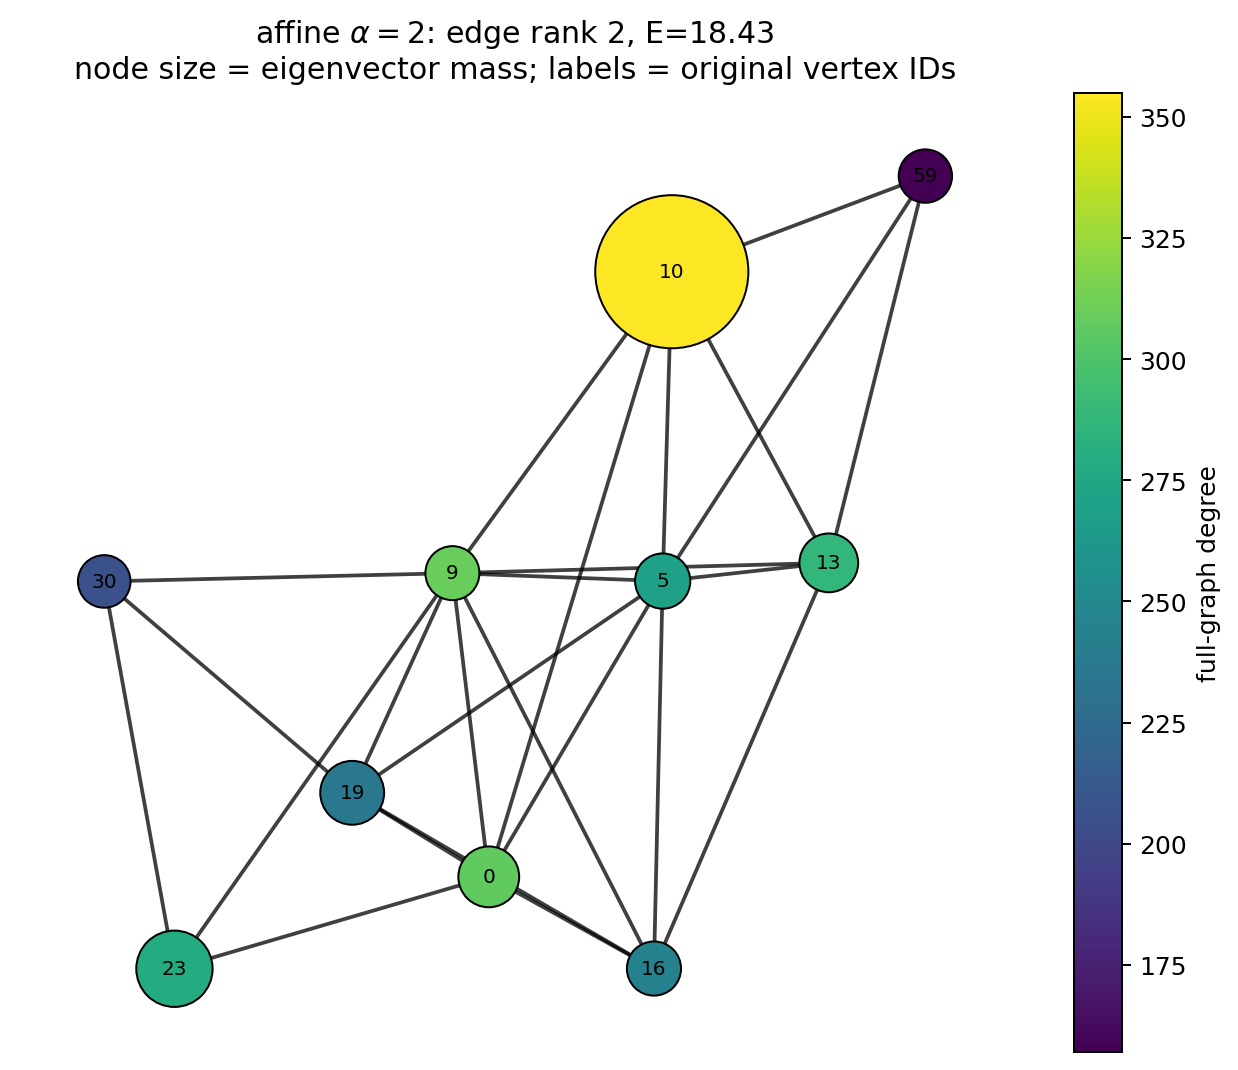
\includegraphics[width=\linewidth]{figures/affine_alpha_2p0/induced_subgraphs/edge/edge_rank_002.png}
\caption*{\footnotesize edge rank 002}\end{minipage}
\par\medskip
\begin{minipage}[t]{.48\linewidth}\centering
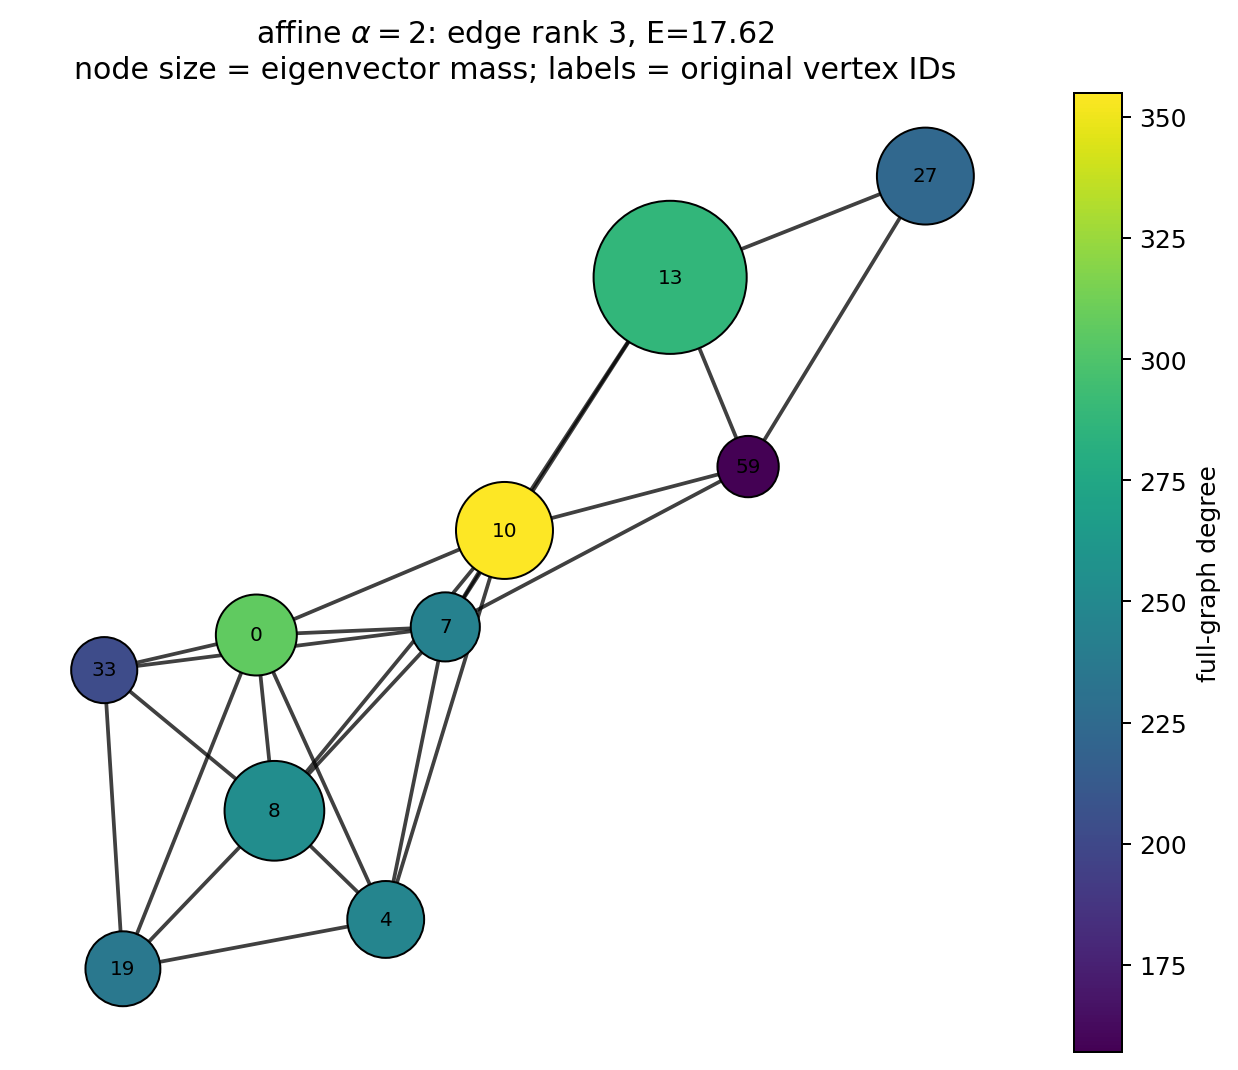
\includegraphics[width=\linewidth]{figures/affine_alpha_2p0/induced_subgraphs/edge/edge_rank_003.png}
\caption*{\footnotesize edge rank 003}\end{minipage}
\hfill
\begin{minipage}[t]{.48\linewidth}\centering
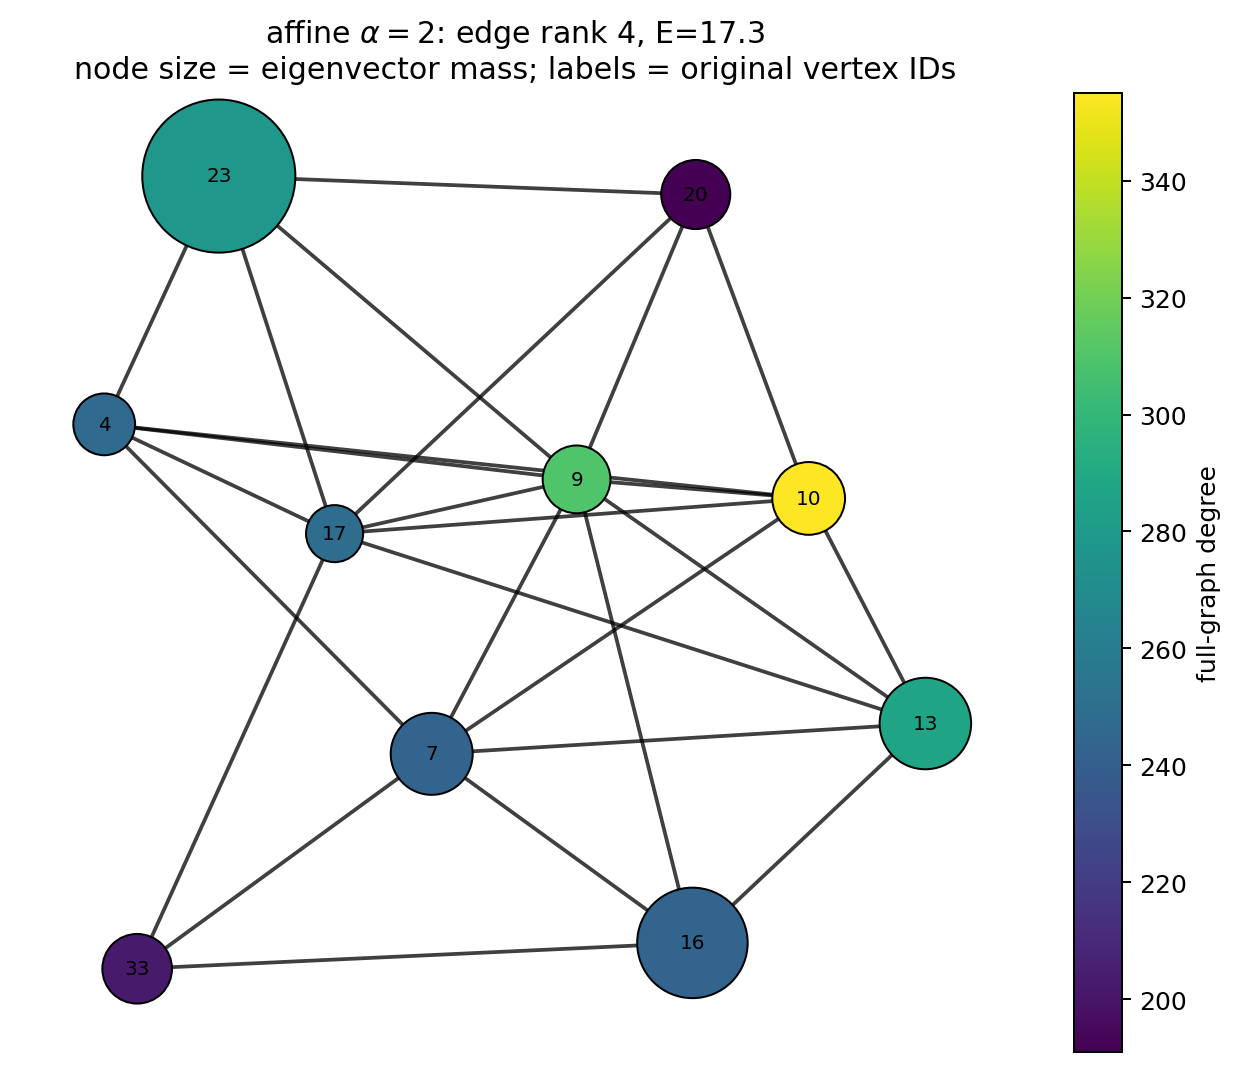
\includegraphics[width=\linewidth]{figures/affine_alpha_2p0/induced_subgraphs/edge/edge_rank_004.png}
\caption*{\footnotesize edge rank 004}\end{minipage}
\caption{Original edge induced supports, ranks 1--4.}\end{figure}
\begin{figure}[H]\centering
\begin{minipage}[t]{.48\linewidth}\centering
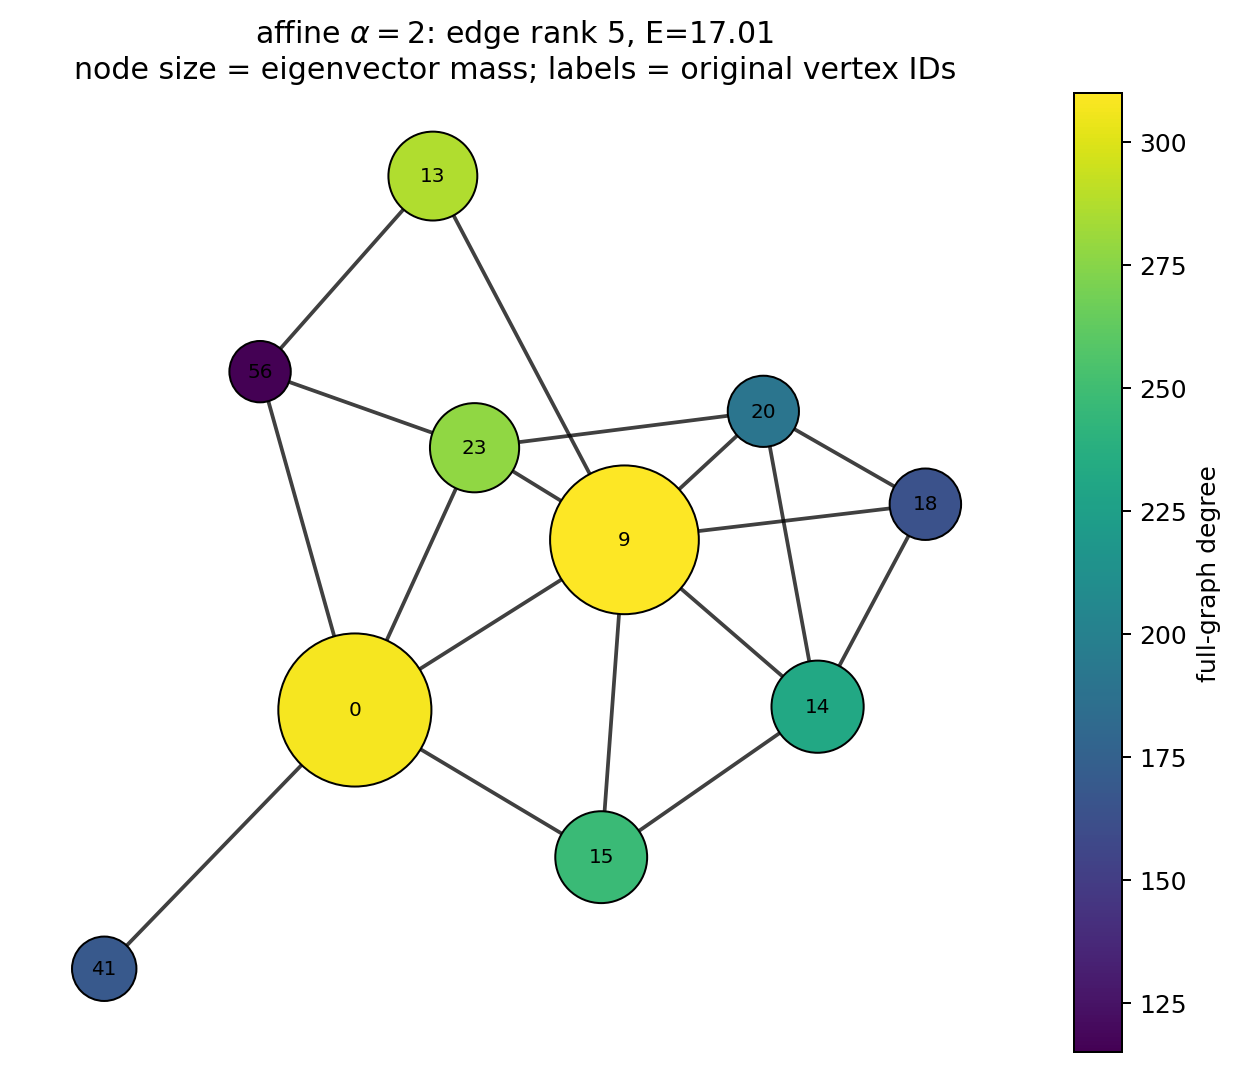
\includegraphics[width=\linewidth]{figures/affine_alpha_2p0/induced_subgraphs/edge/edge_rank_005.png}
\caption*{\footnotesize edge rank 005}\end{minipage}
\hfill
\begin{minipage}[t]{.48\linewidth}\centering
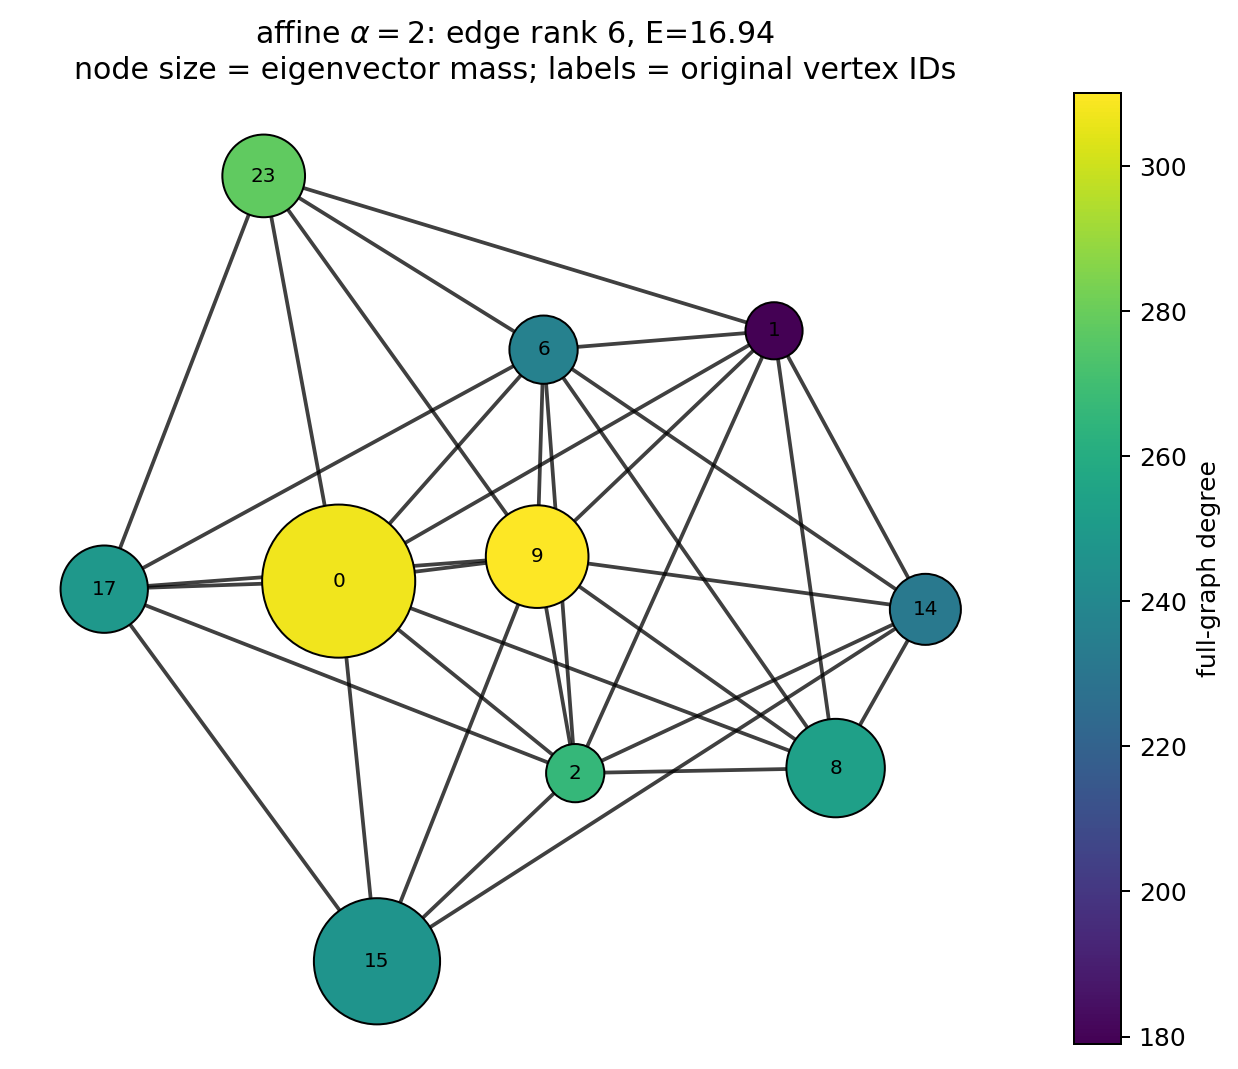
\includegraphics[width=\linewidth]{figures/affine_alpha_2p0/induced_subgraphs/edge/edge_rank_006.png}
\caption*{\footnotesize edge rank 006}\end{minipage}
\par\medskip
\begin{minipage}[t]{.48\linewidth}\centering
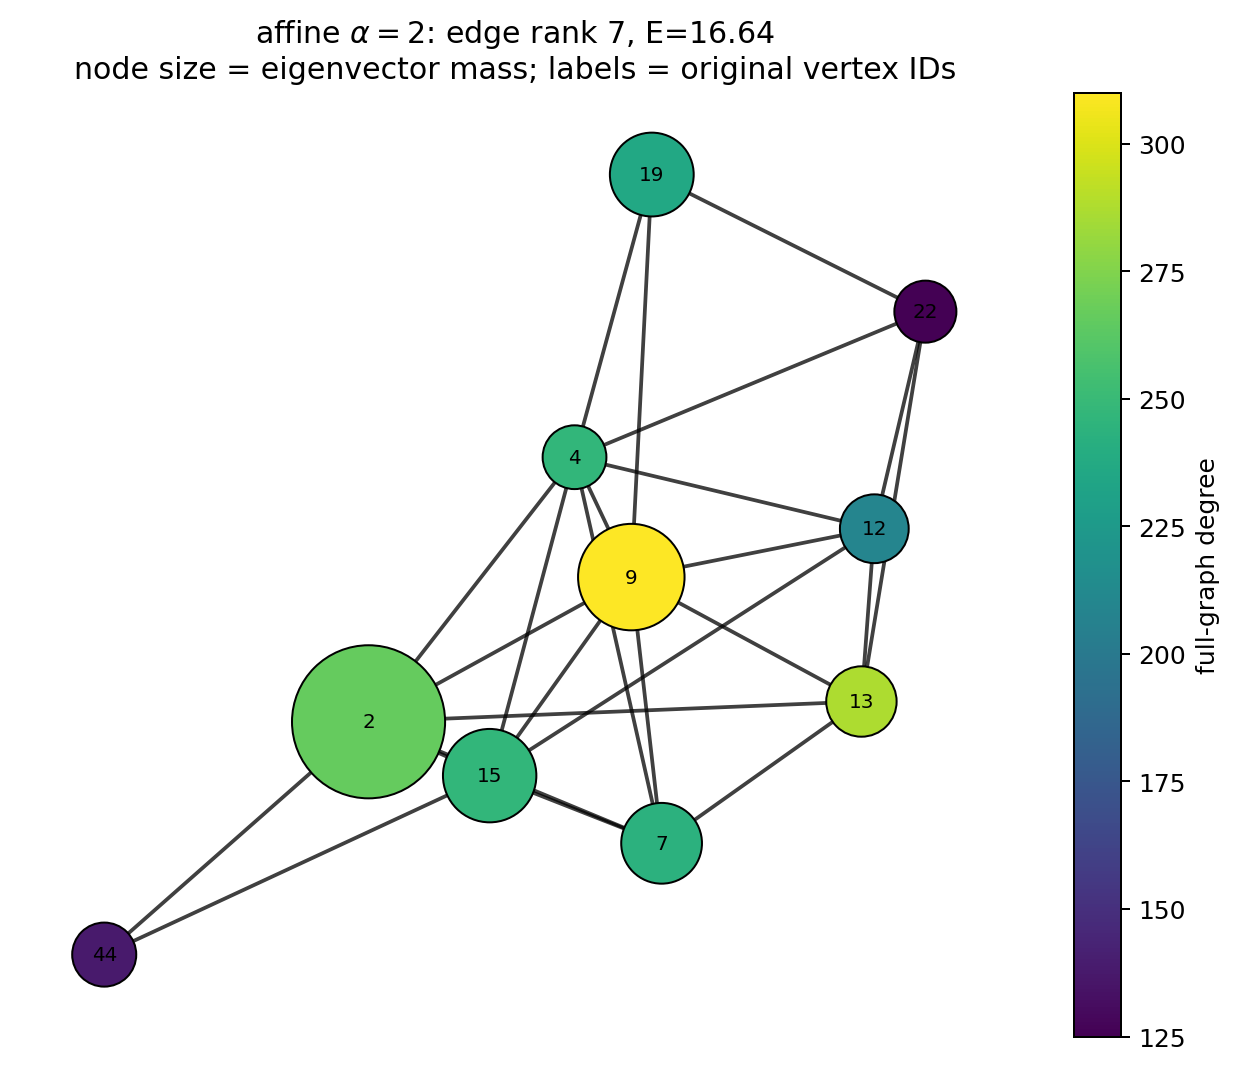
\includegraphics[width=\linewidth]{figures/affine_alpha_2p0/induced_subgraphs/edge/edge_rank_007.png}
\caption*{\footnotesize edge rank 007}\end{minipage}
\hfill
\begin{minipage}[t]{.48\linewidth}\centering
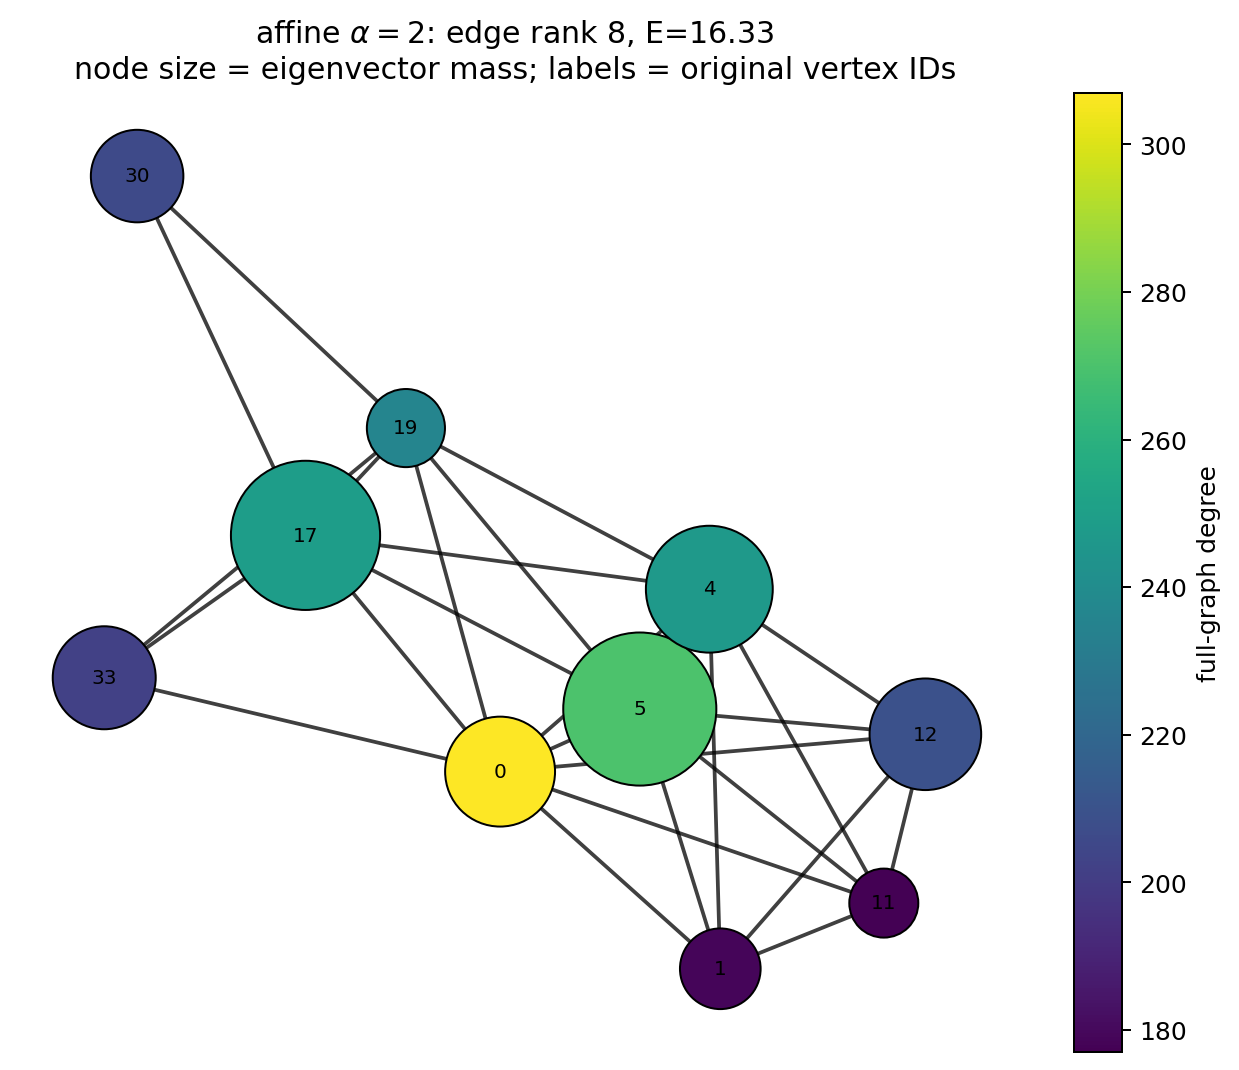
\includegraphics[width=\linewidth]{figures/affine_alpha_2p0/induced_subgraphs/edge/edge_rank_008.png}
\caption*{\footnotesize edge rank 008}\end{minipage}
\caption{Original edge induced supports, ranks 5--8.}\end{figure}
\begin{figure}[H]\centering
\begin{minipage}[t]{.48\linewidth}\centering
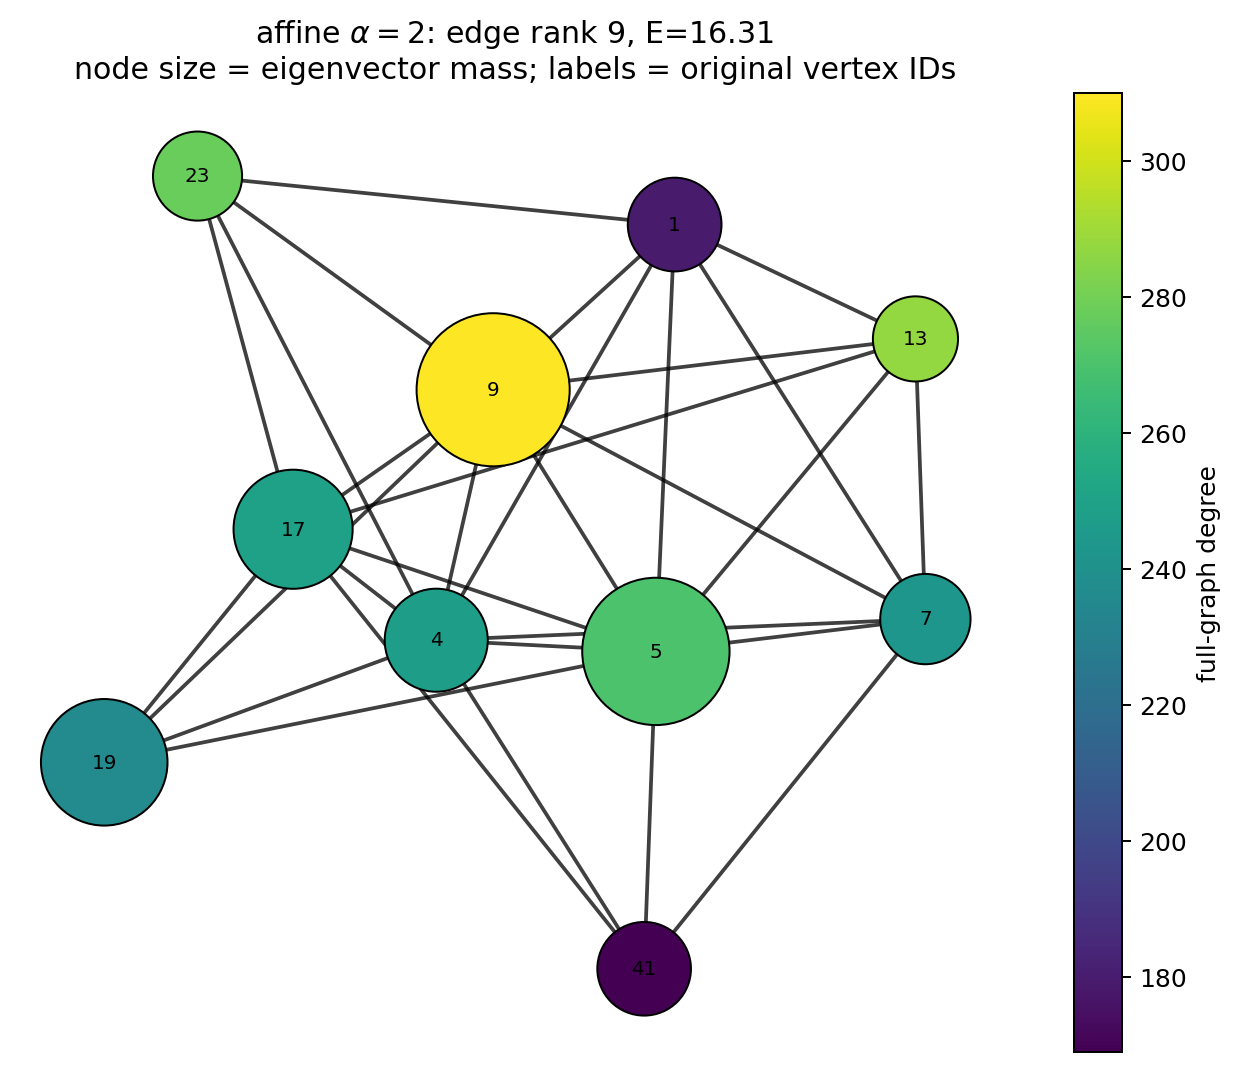
\includegraphics[width=\linewidth]{figures/affine_alpha_2p0/induced_subgraphs/edge/edge_rank_009.png}
\caption*{\footnotesize edge rank 009}\end{minipage}
\hfill
\begin{minipage}[t]{.48\linewidth}\centering
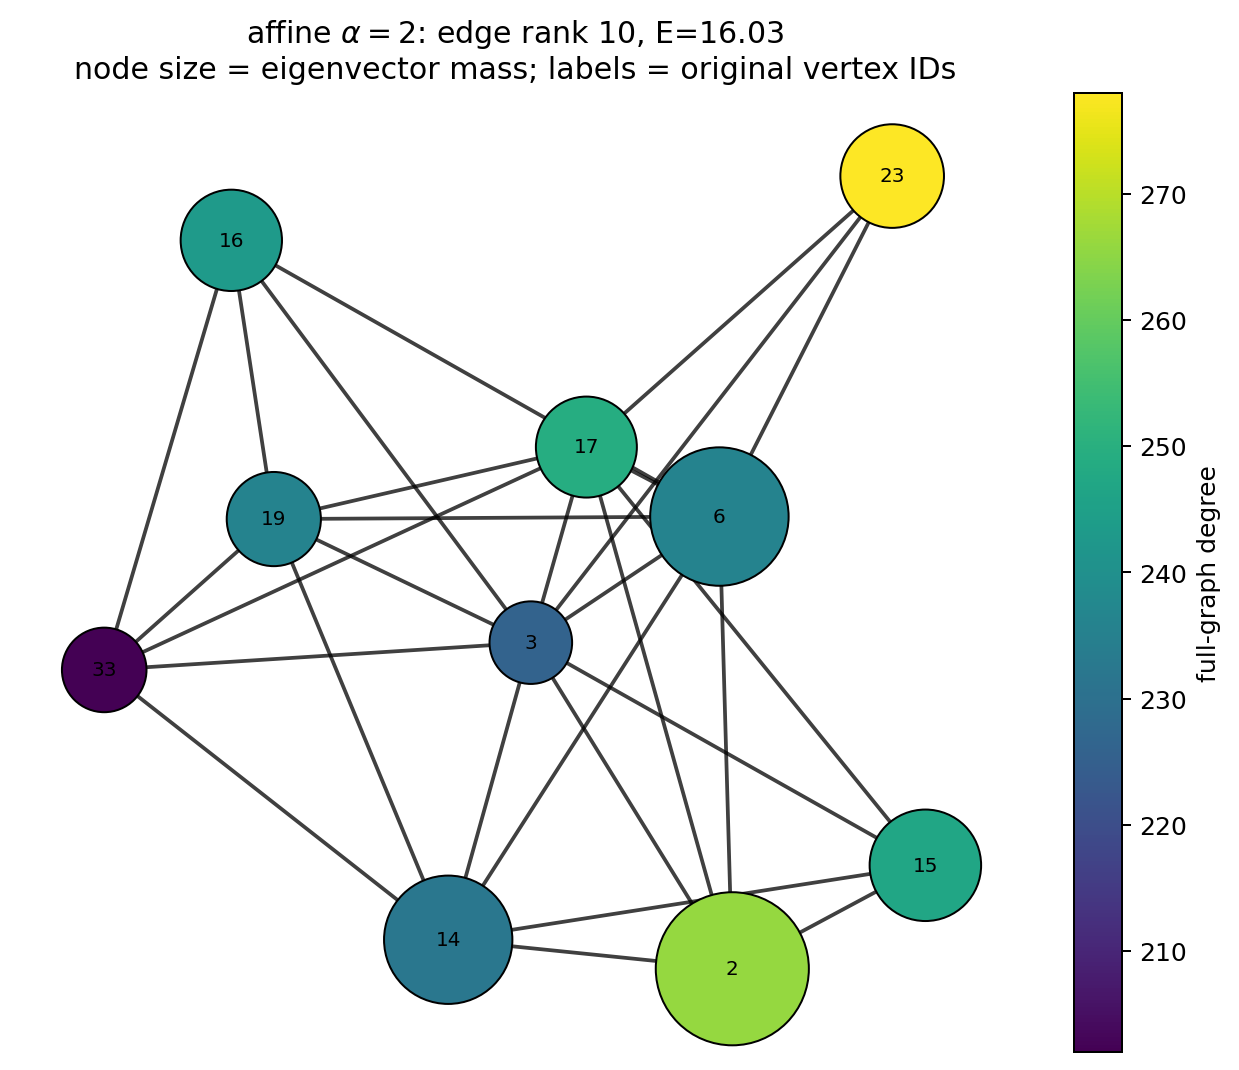
\includegraphics[width=\linewidth]{figures/affine_alpha_2p0/induced_subgraphs/edge/edge_rank_010.png}
\caption*{\footnotesize edge rank 010}\end{minipage}
\caption{Original edge induced supports, ranks 9--10.}\end{figure}
\subsection{affine $\alpha=2.0$: original centered bulk window}
\begin{figure}[H]\centering
\begin{minipage}[t]{.48\linewidth}\centering
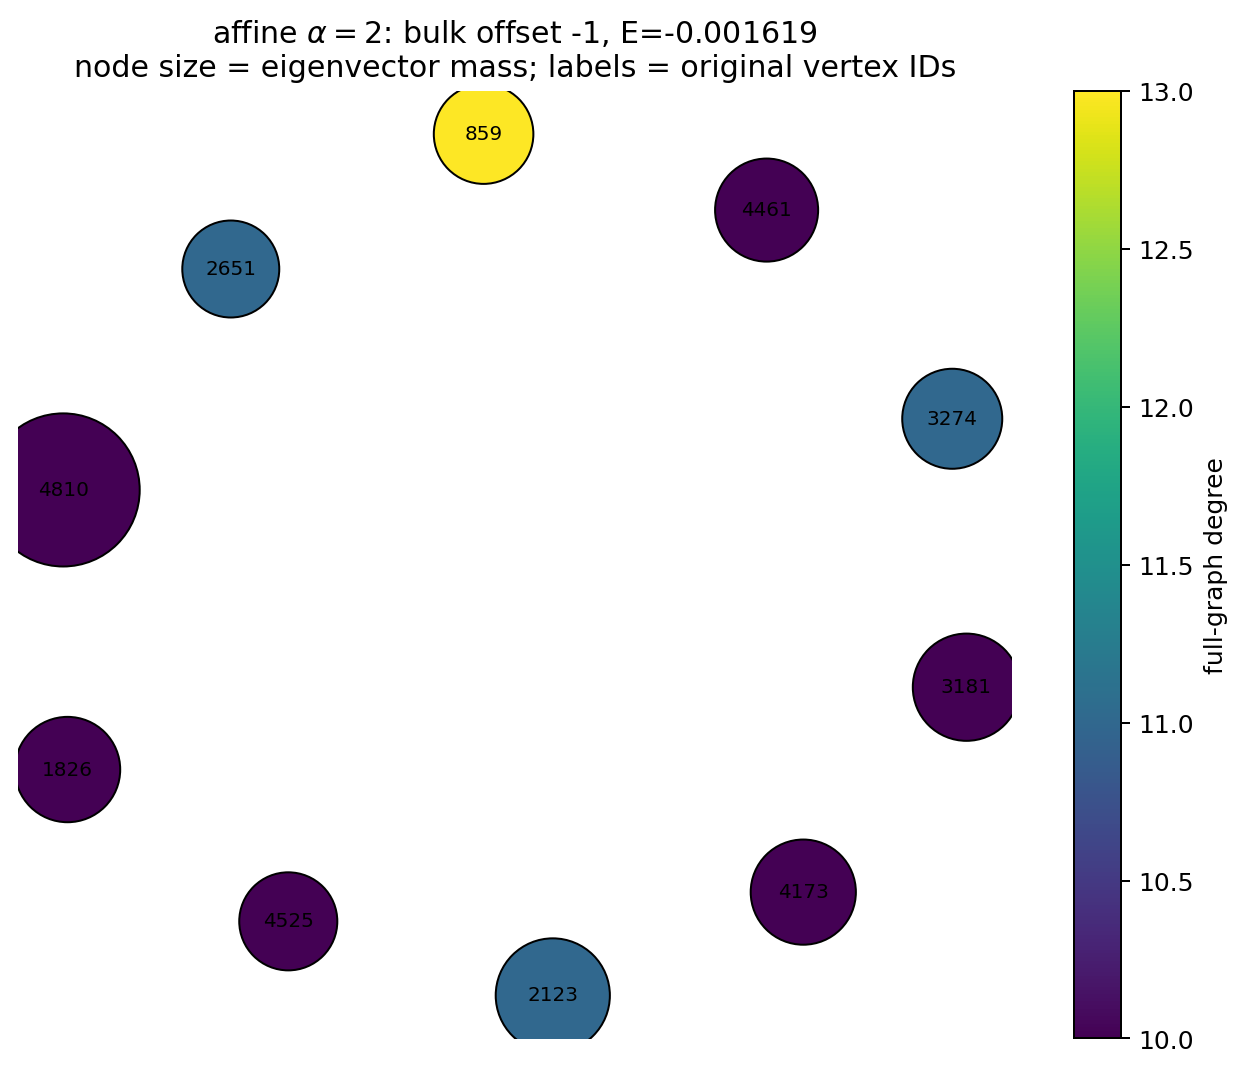
\includegraphics[width=\linewidth]{figures/affine_alpha_2p0/induced_subgraphs/bulk/bulk_offset_m001.png}
\caption*{\footnotesize bulk offset m001}\end{minipage}
\hfill
\begin{minipage}[t]{.48\linewidth}\centering
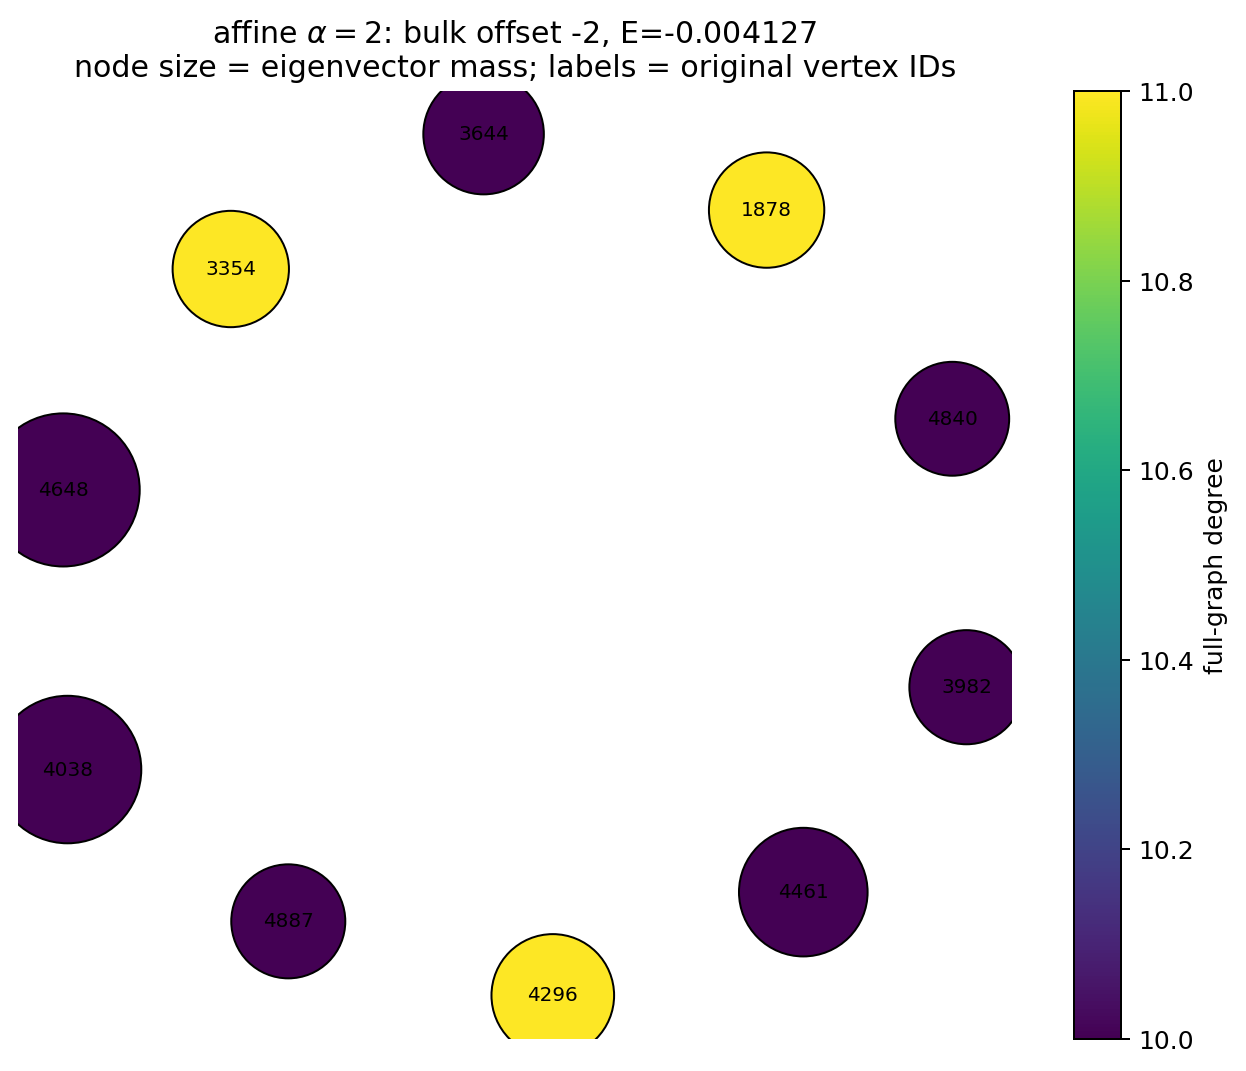
\includegraphics[width=\linewidth]{figures/affine_alpha_2p0/induced_subgraphs/bulk/bulk_offset_m002.png}
\caption*{\footnotesize bulk offset m002}\end{minipage}
\par\medskip
\begin{minipage}[t]{.48\linewidth}\centering
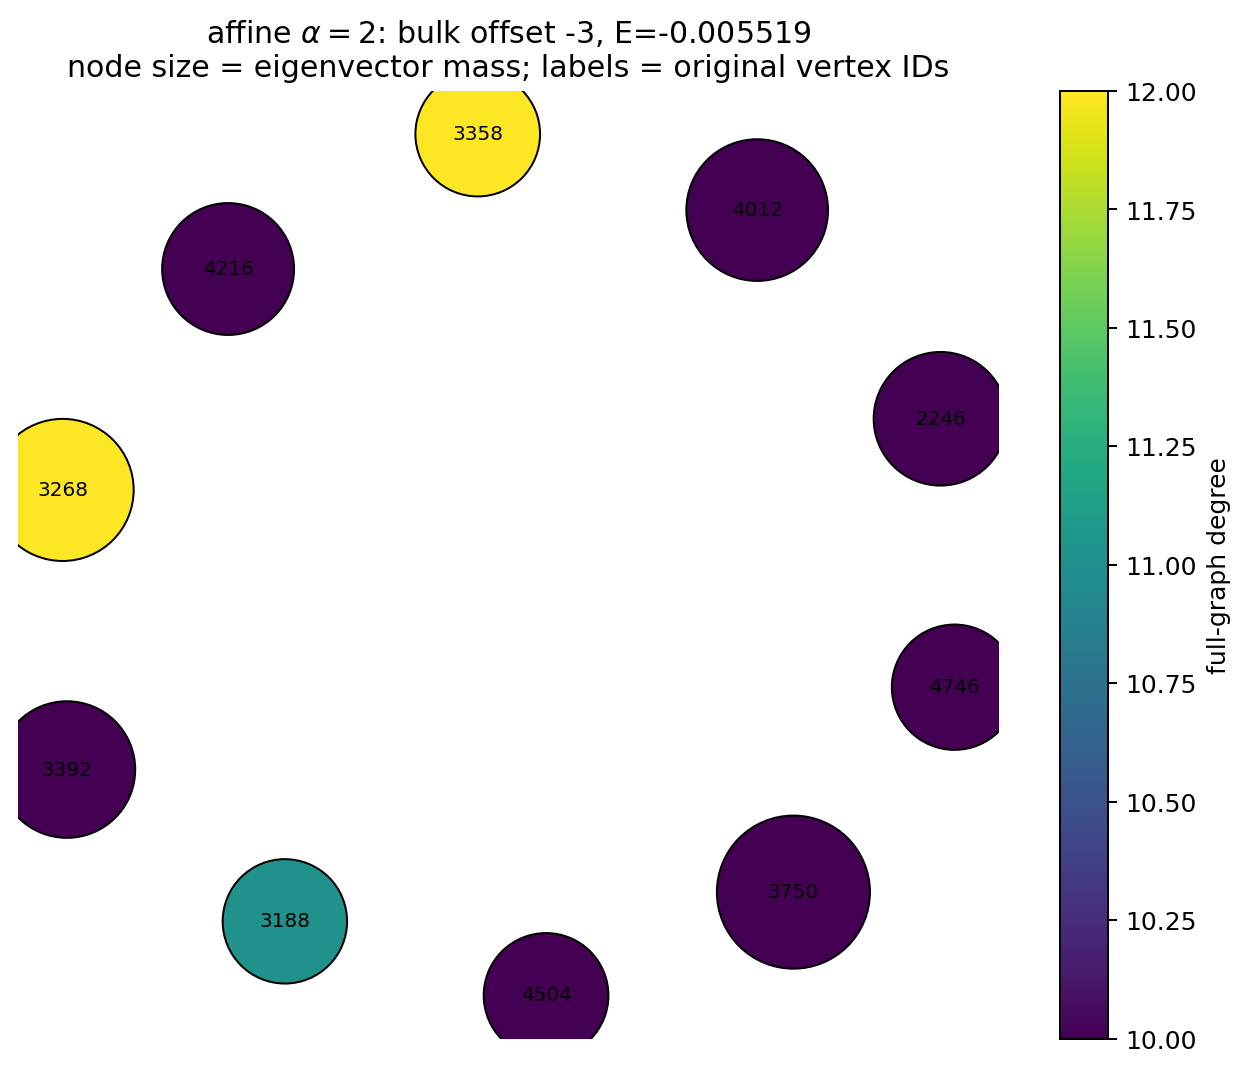
\includegraphics[width=\linewidth]{figures/affine_alpha_2p0/induced_subgraphs/bulk/bulk_offset_m003.png}
\caption*{\footnotesize bulk offset m003}\end{minipage}
\hfill
\begin{minipage}[t]{.48\linewidth}\centering
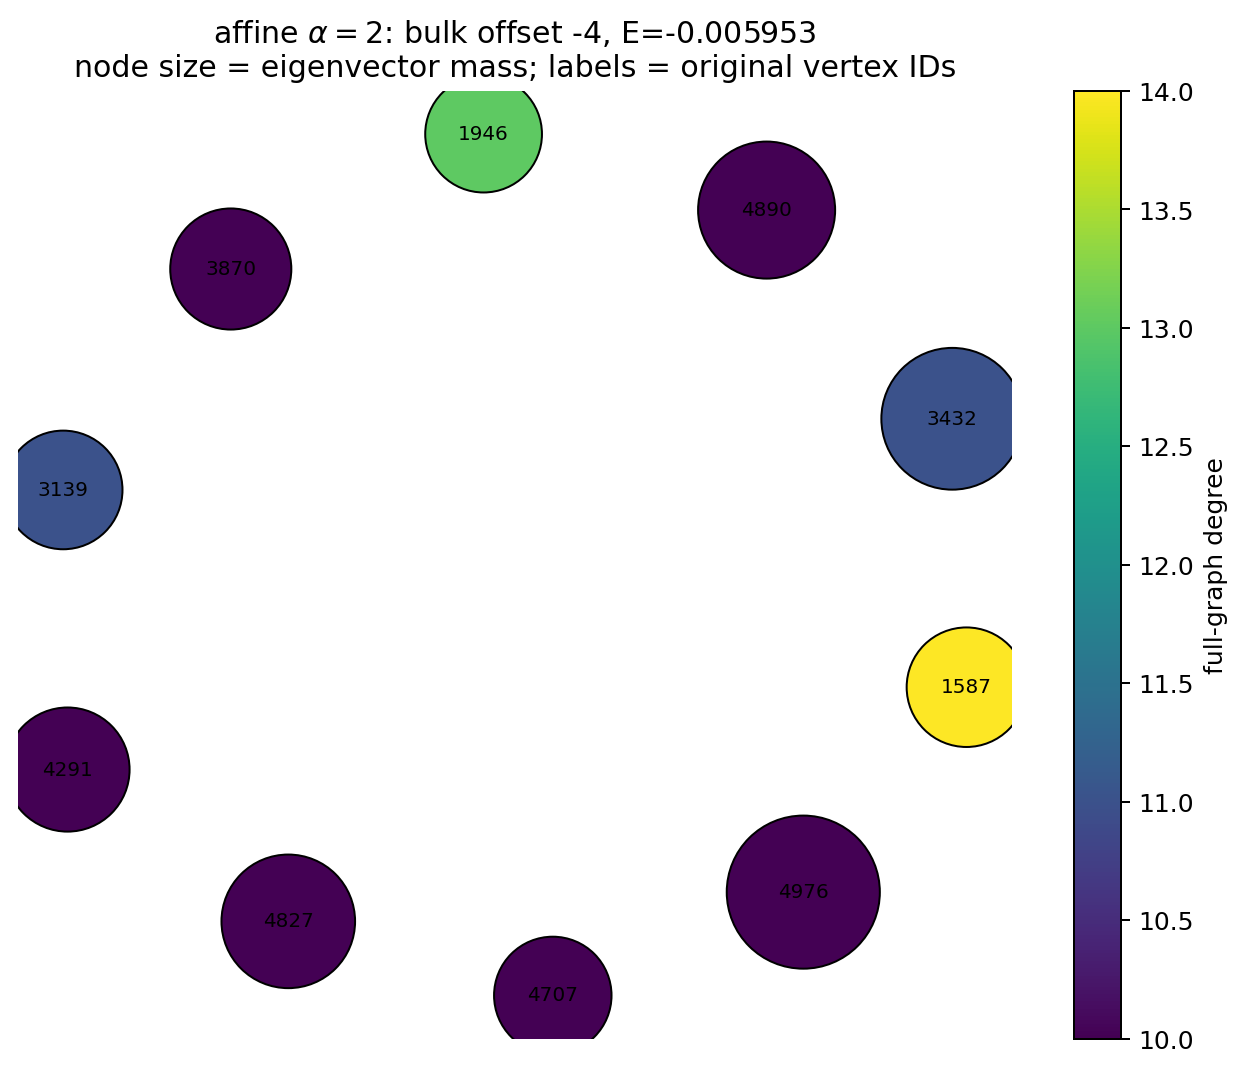
\includegraphics[width=\linewidth]{figures/affine_alpha_2p0/induced_subgraphs/bulk/bulk_offset_m004.png}
\caption*{\footnotesize bulk offset m004}\end{minipage}
\caption{Original centered bulk induced supports.}\end{figure}
\begin{figure}[H]\centering
\begin{minipage}[t]{.48\linewidth}\centering
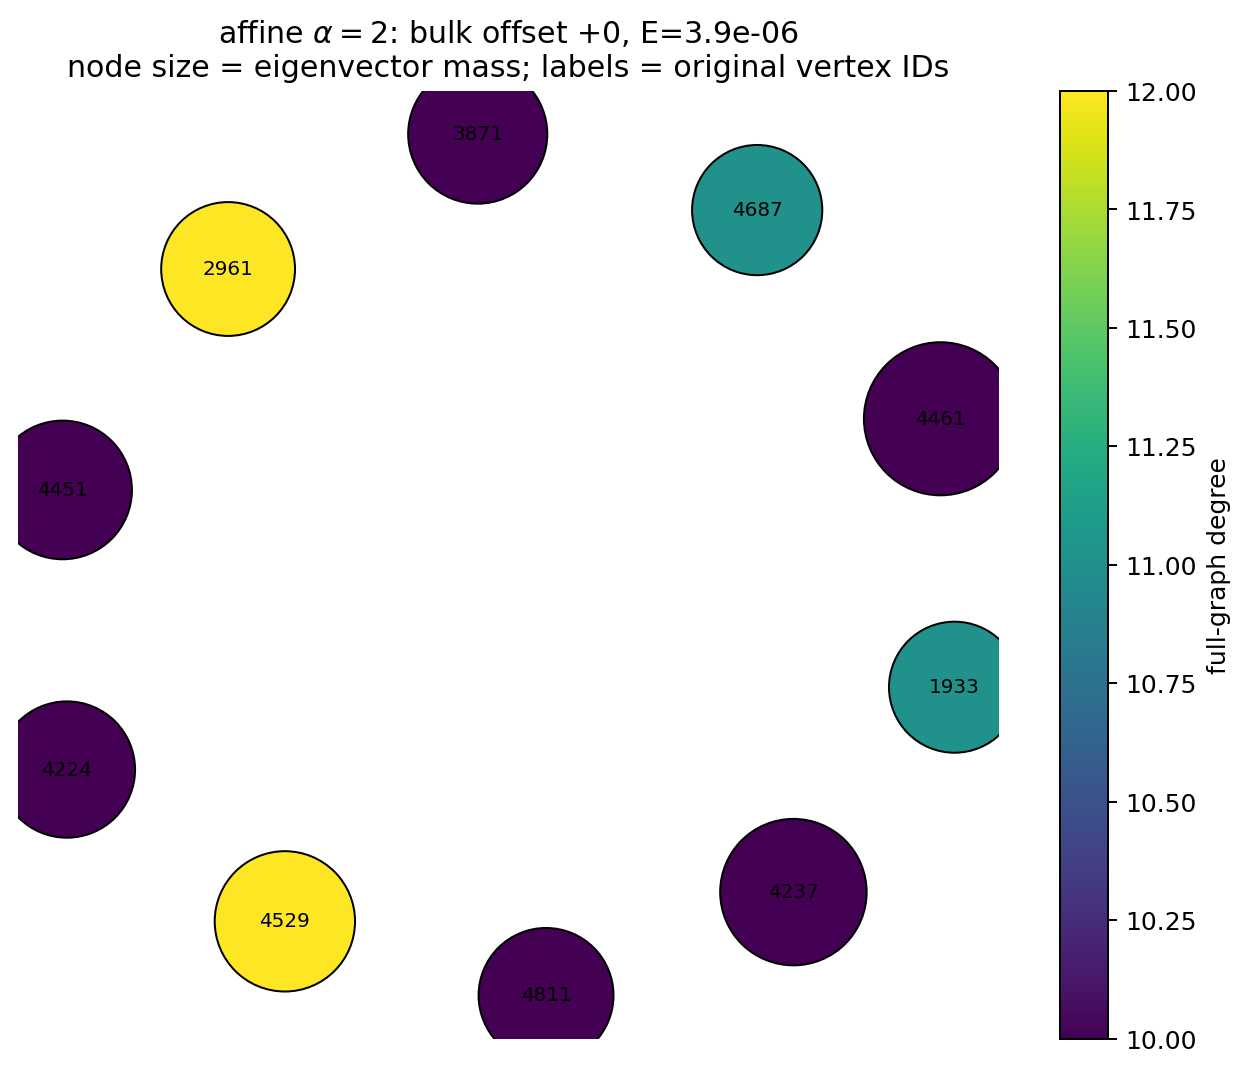
\includegraphics[width=\linewidth]{figures/affine_alpha_2p0/induced_subgraphs/bulk/bulk_offset_p000.png}
\caption*{\footnotesize bulk offset p000}\end{minipage}
\hfill
\begin{minipage}[t]{.48\linewidth}\centering
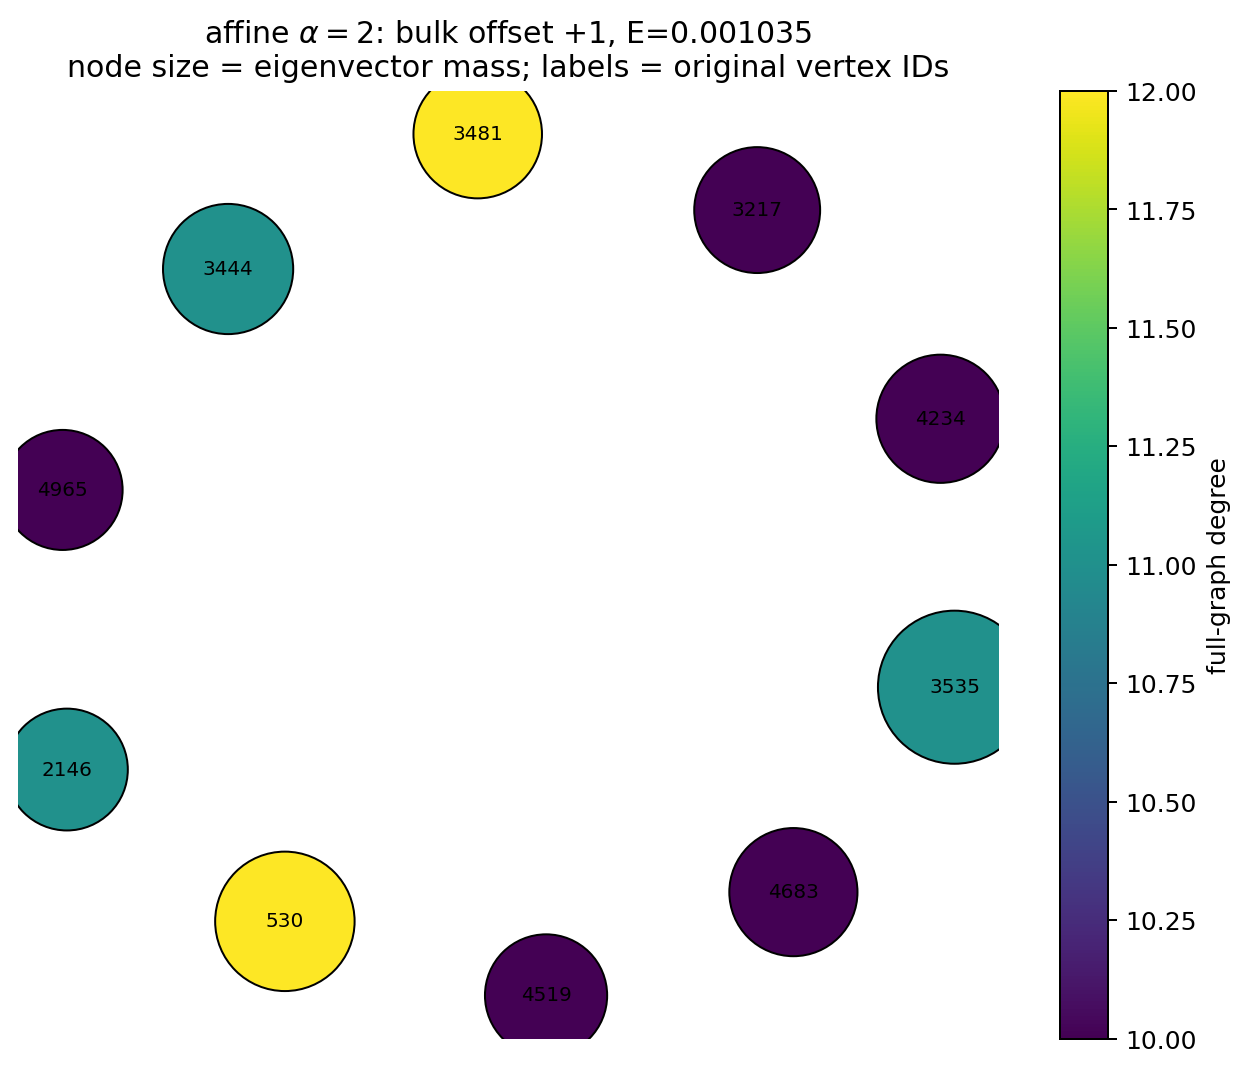
\includegraphics[width=\linewidth]{figures/affine_alpha_2p0/induced_subgraphs/bulk/bulk_offset_p001.png}
\caption*{\footnotesize bulk offset p001}\end{minipage}
\par\medskip
\begin{minipage}[t]{.48\linewidth}\centering
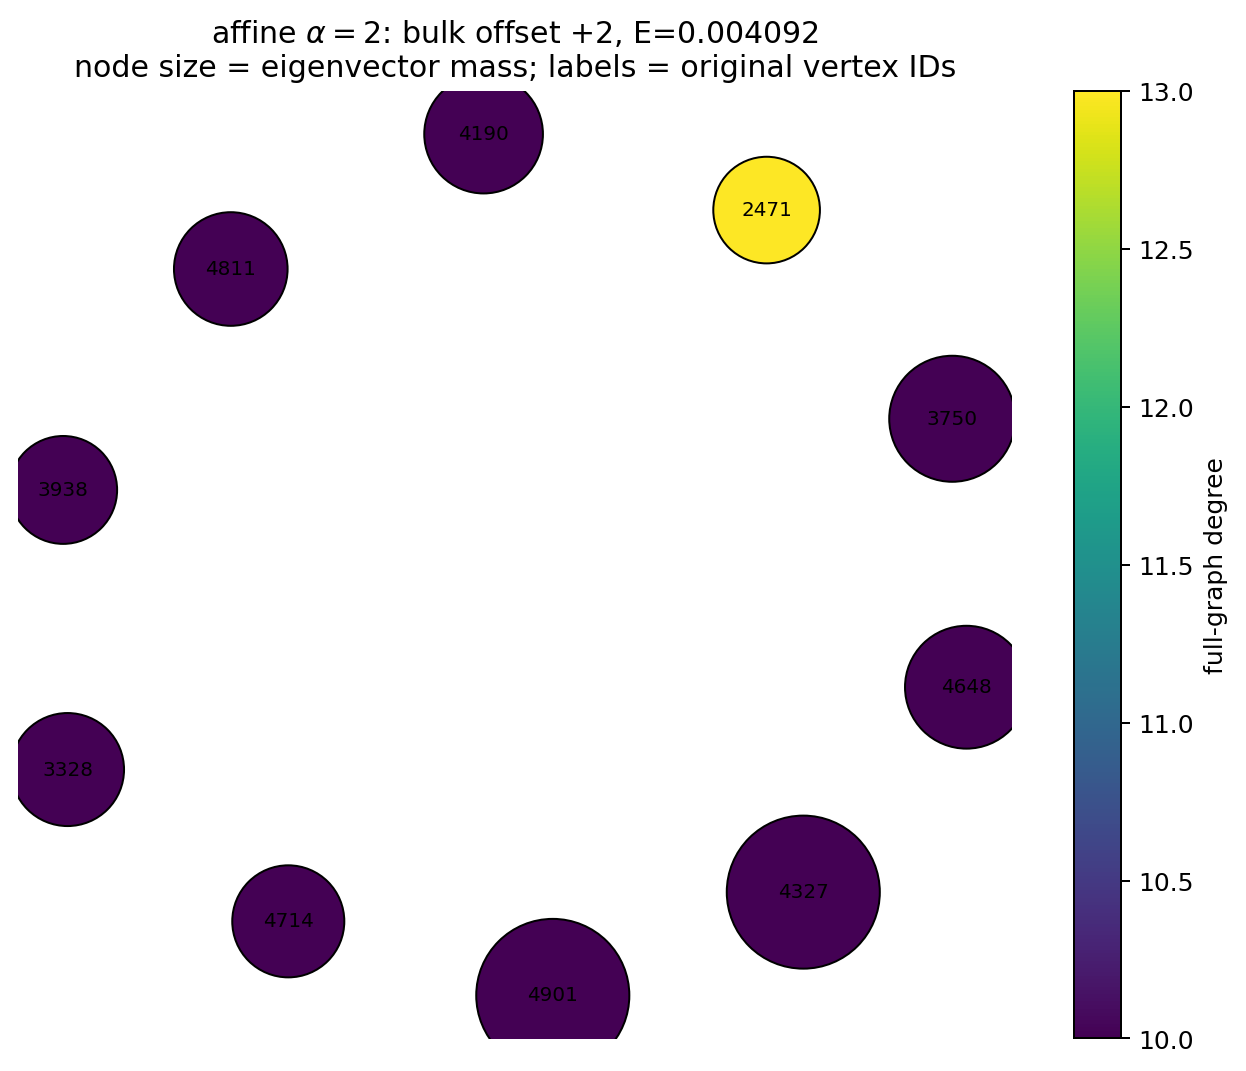
\includegraphics[width=\linewidth]{figures/affine_alpha_2p0/induced_subgraphs/bulk/bulk_offset_p002.png}
\caption*{\footnotesize bulk offset p002}\end{minipage}
\hfill
\begin{minipage}[t]{.48\linewidth}\centering
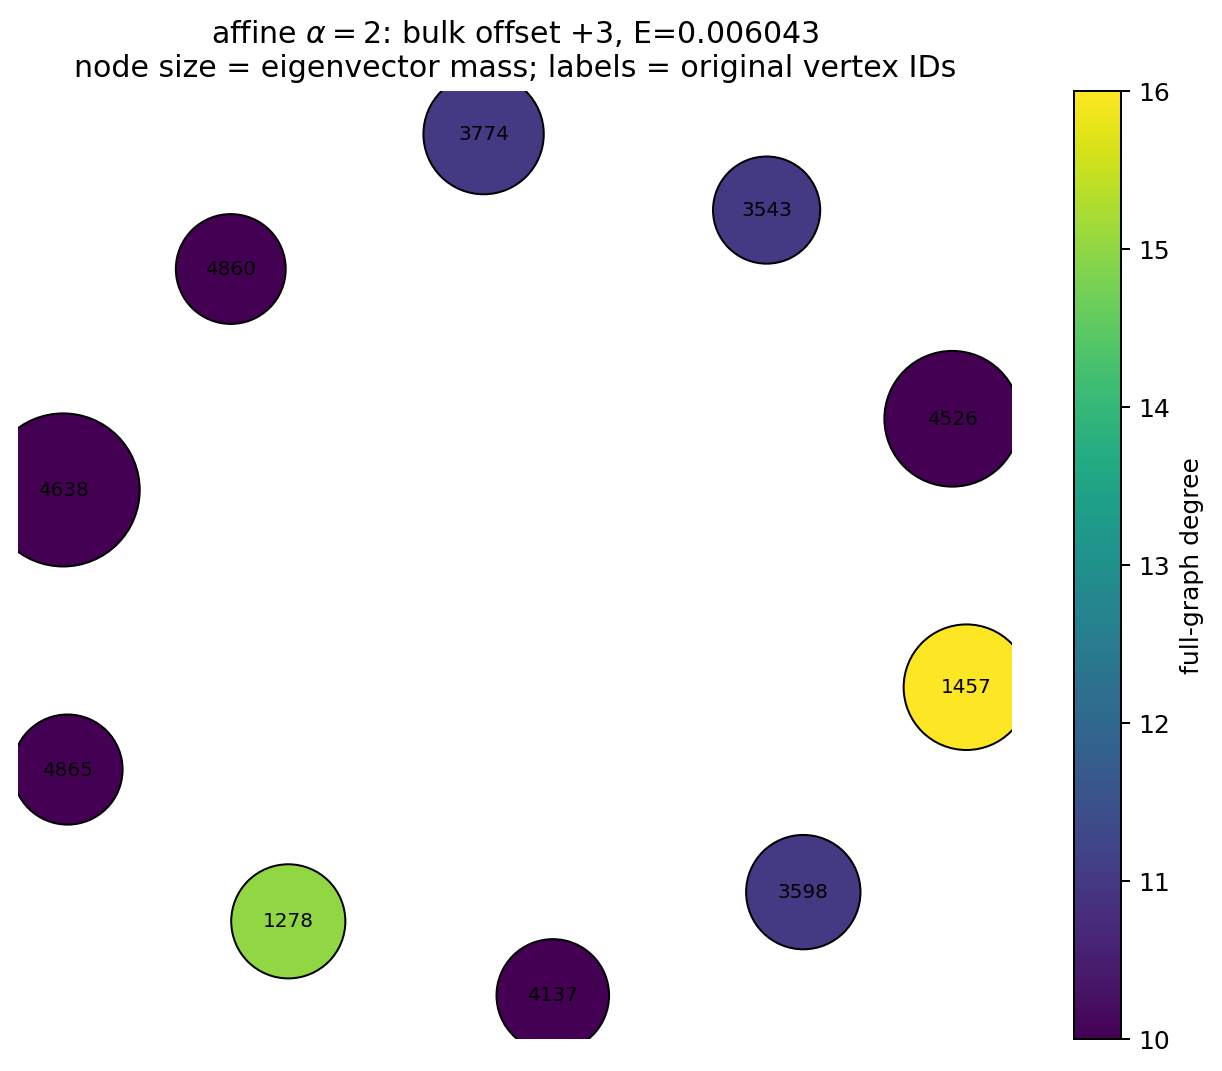
\includegraphics[width=\linewidth]{figures/affine_alpha_2p0/induced_subgraphs/bulk/bulk_offset_p003.png}
\caption*{\footnotesize bulk offset p003}\end{minipage}
\caption{Original centered bulk induced supports.}\end{figure}
\begin{figure}[H]\centering
\begin{minipage}[t]{.48\linewidth}\centering
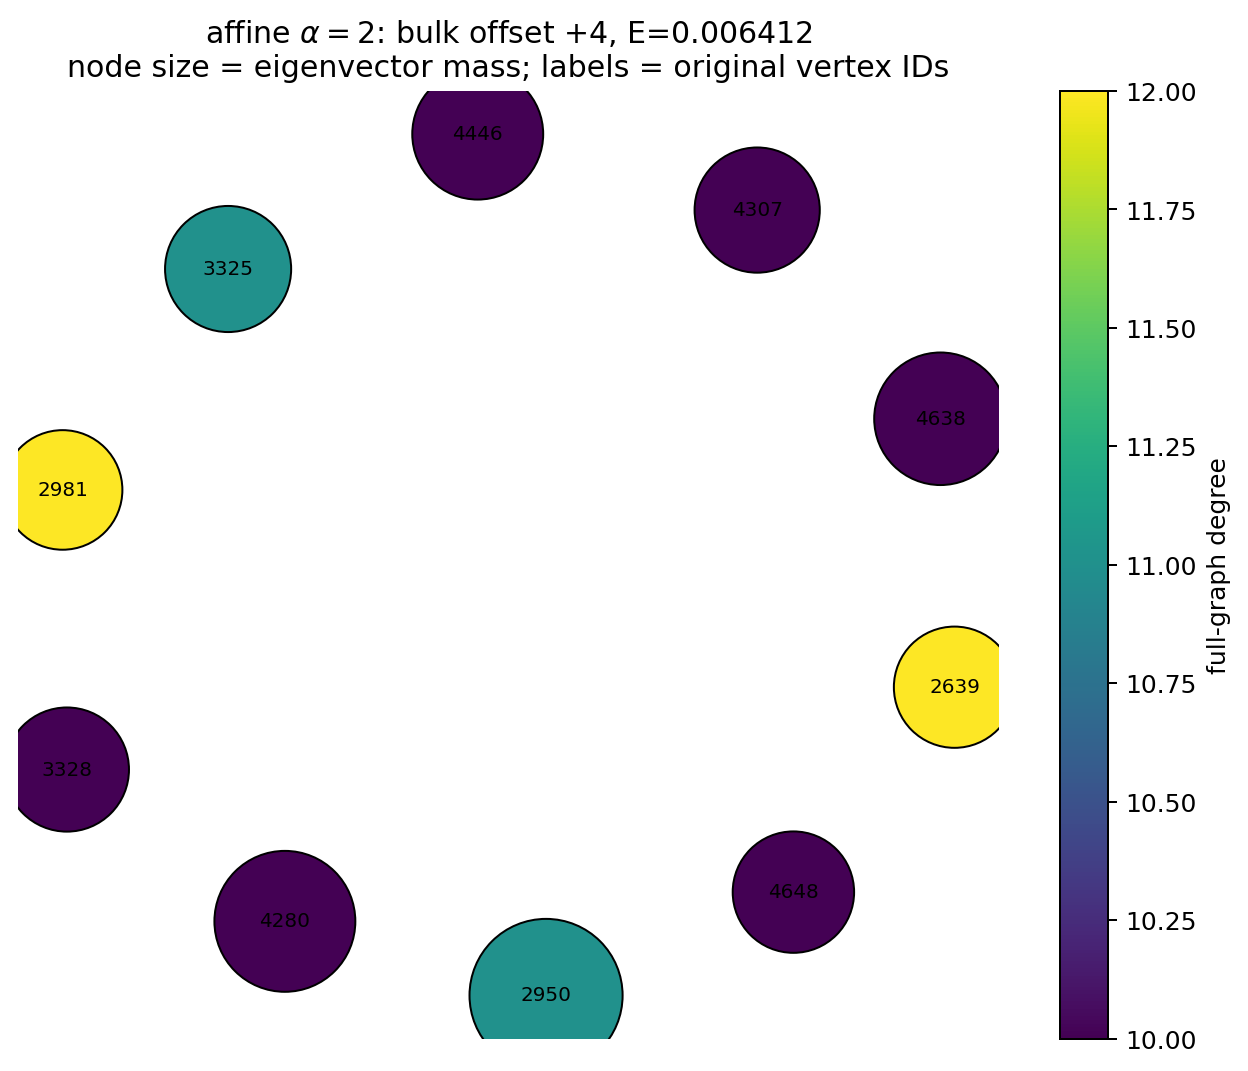
\includegraphics[width=\linewidth]{figures/affine_alpha_2p0/induced_subgraphs/bulk/bulk_offset_p004.png}
\caption*{\footnotesize bulk offset p004}\end{minipage}
\hfill
\begin{minipage}[t]{.48\linewidth}\centering
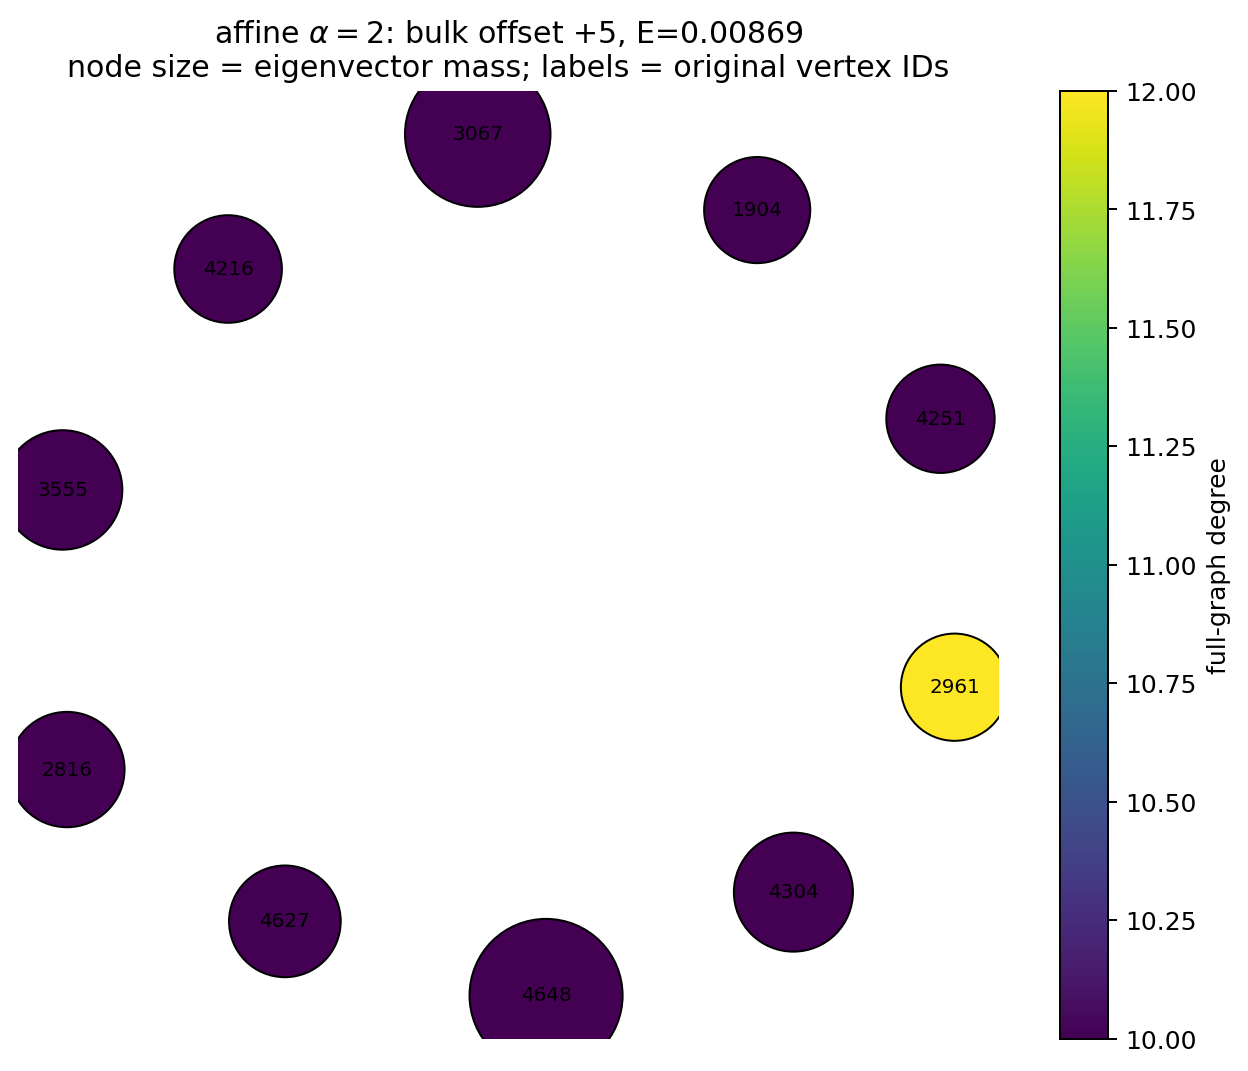
\includegraphics[width=\linewidth]{figures/affine_alpha_2p0/induced_subgraphs/bulk/bulk_offset_p005.png}
\caption*{\footnotesize bulk offset p005}\end{minipage}
\caption{Original centered bulk induced supports.}\end{figure}
\begingroup\section{Explicit figure-file manifest}
Every path below is quoted literally by an \texttt{\textbackslash includegraphics} command and included in the package.
\fontsize{5}{5.8}\selectfont\setlength{\tabcolsep}{2pt}
\rowcolors{2}{white}{lightblue}\begin{longtable}{|p{0.80\linewidth}|r|}\hline
\Hdr{TeX-relative filename} & \Hdr{Bytes} \\\hline\endfirsthead
\hline\Hdr{TeX-relative filename} & \Hdr{Bytes} \\\hline\endhead
\path{figures/affine_alpha_1p05/bulk/bulk_offset_diagnostics.png} & 262825 \\\hline
\path{figures/affine_alpha_1p05/edge/edge_rank_diagnostics.png} & 258409 \\\hline
\path{figures/affine_alpha_1p05/edge_vs_bulk/edge_vs_bulk_comparison.png} & 215279 \\\hline
\path{figures/affine_alpha_1p05/energy_ipr/single_graph_localization_vs_energy.png} & 171636 \\\hline
\path{figures/affine_alpha_1p05/histograms/single_graph_global_spacing_and_ratio.png} & 133652 \\\hline
\path{figures/affine_alpha_1p05/histograms/single_graph_local_raw_spacing_histograms.png} & 273786 \\\hline
\path{figures/affine_alpha_1p05/histograms/single_graph_local_unfolded_spacing_histograms.png} & 315352 \\\hline
\path{figures/affine_alpha_1p05/induced_subgraphs/bulk/bulk_offset_m001.png} & 94609 \\\hline
\path{figures/affine_alpha_1p05/induced_subgraphs/bulk/bulk_offset_m002.png} & 100453 \\\hline
\path{figures/affine_alpha_1p05/induced_subgraphs/bulk/bulk_offset_m003.png} & 95766 \\\hline
\path{figures/affine_alpha_1p05/induced_subgraphs/bulk/bulk_offset_m004.png} & 104272 \\\hline
\path{figures/affine_alpha_1p05/induced_subgraphs/bulk/bulk_offset_p000.png} & 107383 \\\hline
\path{figures/affine_alpha_1p05/induced_subgraphs/bulk/bulk_offset_p001.png} & 100933 \\\hline
\path{figures/affine_alpha_1p05/induced_subgraphs/bulk/bulk_offset_p002.png} & 99618 \\\hline
\path{figures/affine_alpha_1p05/induced_subgraphs/bulk/bulk_offset_p003.png} & 99152 \\\hline
\path{figures/affine_alpha_1p05/induced_subgraphs/bulk/bulk_offset_p004.png} & 97497 \\\hline
\path{figures/affine_alpha_1p05/induced_subgraphs/bulk/bulk_offset_p005.png} & 98119 \\\hline
\path{figures/affine_alpha_1p05/induced_subgraphs/edge/edge_rank_001.png} & 299640 \\\hline
\path{figures/affine_alpha_1p05/induced_subgraphs/edge/edge_rank_002.png} & 236160 \\\hline
\path{figures/affine_alpha_1p05/induced_subgraphs/edge/edge_rank_003.png} & 268740 \\\hline
\path{figures/affine_alpha_1p05/induced_subgraphs/edge/edge_rank_004.png} & 262172 \\\hline
\path{figures/affine_alpha_1p05/induced_subgraphs/edge/edge_rank_005.png} & 283889 \\\hline
\path{figures/affine_alpha_1p05/induced_subgraphs/edge/edge_rank_006.png} & 211304 \\\hline
\path{figures/affine_alpha_1p05/induced_subgraphs/edge/edge_rank_007.png} & 232232 \\\hline
\path{figures/affine_alpha_1p05/induced_subgraphs/edge/edge_rank_008.png} & 238807 \\\hline
\path{figures/affine_alpha_1p05/induced_subgraphs/edge/edge_rank_009.png} & 290671 \\\hline
\path{figures/affine_alpha_1p05/induced_subgraphs/edge/edge_rank_010.png} & 218398 \\\hline
\path{figures/affine_alpha_1p05/spectrum/single_graph_eigenvalue_density.png} & 75683 \\\hline
\path{figures/affine_alpha_2p0/bulk/bulk_offset_diagnostics.png} & 255123 \\\hline
\path{figures/affine_alpha_2p0/edge/edge_rank_diagnostics.png} & 256857 \\\hline
\path{figures/affine_alpha_2p0/edge_vs_bulk/edge_vs_bulk_comparison.png} & 191169 \\\hline
\path{figures/affine_alpha_2p0/energy_ipr/single_graph_localization_vs_energy.png} & 147042 \\\hline
\path{figures/affine_alpha_2p0/histograms/single_graph_global_spacing_and_ratio.png} & 150494 \\\hline
\path{figures/affine_alpha_2p0/histograms/single_graph_local_raw_spacing_histograms.png} & 327139 \\\hline
\path{figures/affine_alpha_2p0/histograms/single_graph_local_unfolded_spacing_histograms.png} & 327407 \\\hline
\path{figures/affine_alpha_2p0/induced_subgraphs/bulk/bulk_offset_m001.png} & 96117 \\\hline
\path{figures/affine_alpha_2p0/induced_subgraphs/bulk/bulk_offset_m002.png} & 99902 \\\hline
\path{figures/affine_alpha_2p0/induced_subgraphs/bulk/bulk_offset_m003.png} & 107905 \\\hline
\path{figures/affine_alpha_2p0/induced_subgraphs/bulk/bulk_offset_m004.png} & 104920 \\\hline
\path{figures/affine_alpha_2p0/induced_subgraphs/bulk/bulk_offset_p000.png} & 108098 \\\hline
\path{figures/affine_alpha_2p0/induced_subgraphs/bulk/bulk_offset_p001.png} & 106789 \\\hline
\path{figures/affine_alpha_2p0/induced_subgraphs/bulk/bulk_offset_p002.png} & 97954 \\\hline
\path{figures/affine_alpha_2p0/induced_subgraphs/bulk/bulk_offset_p003.png} & 96720 \\\hline
\path{figures/affine_alpha_2p0/induced_subgraphs/bulk/bulk_offset_p004.png} & 107718 \\\hline
\path{figures/affine_alpha_2p0/induced_subgraphs/bulk/bulk_offset_p005.png} & 102979 \\\hline
\path{figures/affine_alpha_2p0/induced_subgraphs/edge/edge_rank_001.png} & 246894 \\\hline
\path{figures/affine_alpha_2p0/induced_subgraphs/edge/edge_rank_002.png} & 156229 \\\hline
\path{figures/affine_alpha_2p0/induced_subgraphs/edge/edge_rank_003.png} & 134637 \\\hline
\path{figures/affine_alpha_2p0/induced_subgraphs/edge/edge_rank_004.png} & 176360 \\\hline
\path{figures/affine_alpha_2p0/induced_subgraphs/edge/edge_rank_005.png} & 133442 \\\hline
\path{figures/affine_alpha_2p0/induced_subgraphs/edge/edge_rank_006.png} & 212213 \\\hline
\path{figures/affine_alpha_2p0/induced_subgraphs/edge/edge_rank_007.png} & 142883 \\\hline
\path{figures/affine_alpha_2p0/induced_subgraphs/edge/edge_rank_008.png} & 160499 \\\hline
\path{figures/affine_alpha_2p0/induced_subgraphs/edge/edge_rank_009.png} & 189595 \\\hline
\path{figures/affine_alpha_2p0/induced_subgraphs/edge/edge_rank_010.png} & 192340 \\\hline
\path{figures/affine_alpha_2p0/spectrum/single_graph_eigenvalue_density.png} & 63285 \\\hline
\path{figures/nonlinear_zeta_1p5/bulk/bulk_offset_diagnostics.png} & 256403 \\\hline
\path{figures/nonlinear_zeta_1p5/edge/edge_rank_diagnostics.png} & 259680 \\\hline
\path{figures/nonlinear_zeta_1p5/edge_vs_bulk/edge_vs_bulk_comparison.png} & 185800 \\\hline
\path{figures/nonlinear_zeta_1p5/energy_ipr/single_graph_localization_vs_energy.png} & 142161 \\\hline
\path{figures/nonlinear_zeta_1p5/histograms/single_graph_global_spacing_and_ratio.png} & 133472 \\\hline
\path{figures/nonlinear_zeta_1p5/histograms/single_graph_local_raw_spacing_histograms.png} & 264631 \\\hline
\path{figures/nonlinear_zeta_1p5/histograms/single_graph_local_unfolded_spacing_histograms.png} & 331044 \\\hline
\path{figures/nonlinear_zeta_1p5/induced_subgraphs/bulk/bulk_offset_m001.png} & 109974 \\\hline
\path{figures/nonlinear_zeta_1p5/induced_subgraphs/bulk/bulk_offset_m002.png} & 97730 \\\hline
\path{figures/nonlinear_zeta_1p5/induced_subgraphs/bulk/bulk_offset_m003.png} & 110125 \\\hline
\path{figures/nonlinear_zeta_1p5/induced_subgraphs/bulk/bulk_offset_m004.png} & 98946 \\\hline
\path{figures/nonlinear_zeta_1p5/induced_subgraphs/bulk/bulk_offset_p000.png} & 99044 \\\hline
\path{figures/nonlinear_zeta_1p5/induced_subgraphs/bulk/bulk_offset_p001.png} & 96876 \\\hline
\path{figures/nonlinear_zeta_1p5/induced_subgraphs/bulk/bulk_offset_p002.png} & 94919 \\\hline
\path{figures/nonlinear_zeta_1p5/induced_subgraphs/bulk/bulk_offset_p003.png} & 105800 \\\hline
\path{figures/nonlinear_zeta_1p5/induced_subgraphs/bulk/bulk_offset_p004.png} & 96375 \\\hline
\path{figures/nonlinear_zeta_1p5/induced_subgraphs/bulk/bulk_offset_p005.png} & 95024 \\\hline
\path{figures/nonlinear_zeta_1p5/induced_subgraphs/edge/edge_rank_001.png} & 288230 \\\hline
\path{figures/nonlinear_zeta_1p5/induced_subgraphs/edge/edge_rank_002.png} & 267793 \\\hline
\path{figures/nonlinear_zeta_1p5/induced_subgraphs/edge/edge_rank_003.png} & 293516 \\\hline
\path{figures/nonlinear_zeta_1p5/induced_subgraphs/edge/edge_rank_004.png} & 185596 \\\hline
\path{figures/nonlinear_zeta_1p5/induced_subgraphs/edge/edge_rank_005.png} & 203804 \\\hline
\path{figures/nonlinear_zeta_1p5/induced_subgraphs/edge/edge_rank_006.png} & 237288 \\\hline
\path{figures/nonlinear_zeta_1p5/induced_subgraphs/edge/edge_rank_007.png} & 272845 \\\hline
\path{figures/nonlinear_zeta_1p5/induced_subgraphs/edge/edge_rank_008.png} & 259188 \\\hline
\path{figures/nonlinear_zeta_1p5/induced_subgraphs/edge/edge_rank_009.png} & 264446 \\\hline
\path{figures/nonlinear_zeta_1p5/induced_subgraphs/edge/edge_rank_010.png} & 271762 \\\hline
\path{figures/nonlinear_zeta_1p5/spectrum/single_graph_eigenvalue_density.png} & 78462 \\\hline
\end{longtable}\endgroup
\section{Machine-readable outputs and limitations}
\begin{itemize}
\item \texttt{tables/window\_summary.csv}: all means and medians.
\item \texttt{tables/random\_1000\_summary.csv}: 1,000-set reference distributions.
\item \texttt{tables/rank51\_sparse\_validation.csv}: disclosed extension validation.
\item \texttt{figure\_manifest.csv} and \texttt{FIGURES.md}: exact filenames and hashes.
\end{itemize}
No new graph ensemble, uncertainty analysis, finite-size scaling, degree-matched null, or parameter sweep was run.
\end{document}
